\documentclass[12pt, a4paper, oneside, notitlepage]{report}
%\documentclass[12pt, a4paper, oneside, notitlepage, draft]{report}

%\usepackage[utf8]{inputenc}
\usepackage{amsmath}
\usepackage{amsfonts}
\usepackage{amssymb}
\usepackage{graphicx}
\usepackage[left=1.5cm, right=5cm, bottom = 1cm, top = 2cm, headheight=16pt,
headsep = 0.5cm, foot = 16pt, footskip = 0.5cm]{geometry}
\setlength{\marginparwidth}{4.5cm}
\usepackage{marginnote}

\usepackage{fontspec}
\setmainfont{Charis SIL}
\usepackage{setspace}
\setstretch{1.1}
\usepackage[french]{babel}
\usepackage[babel=true]{csquotes}

\usepackage{soul}
\usepackage{mdframed}

\usepackage{xargs} % Use more than one optional parameter in a new commands
\usepackage[dvipsnames]{xcolor}


\usepackage{float}
\usepackage{caption}
\captionsetup[figure]{belowskip=-0.5cm}
\captionsetup[lstlisting]{belowskip=-0.25cm}
%\captionsetup[table]{position=above, aboveskip=0pt, belowskip=10pt}
\usepackage{rotating}
\usepackage{rotfloat}

\usepackage{fancyhdr}
\pagestyle{fancy}

\renewcommand{\headrulewidth}{0.5pt}
\renewcommand{\footrulewidth}{0pt}
\fancyhead[L]{Chapitre \thechapter}
\fancyhead[C]{}
\fancyhead[R]{\rightmark}

\usepackage{epigraph}

\newcounter{savefootnote}
\renewcommand{\thempfootnote}{\arabic{footnote}}%

\usepackage{enumitem}

\usepackage[hyperfootnotes=false]{hyperref}
\hypersetup{pdftitle={Robin Cura - Thèse}}
\usepackage[noabbrev, nameinlink]{cleveref}

\usepackage{longtable}
\usepackage{array}

\usepackage{fontawesome}
\usepackage{wrapfig}
\usepackage[style=authoryear-comp,
hyperref,
backend=bibtex,
isbn=false,
doi=true,
url=true,
date=year,
sortcites=false,  % Ne pas changer l'ordre des citations multiples
sorting=nyt % Citations dans biblio : NameYearTitle
]{biblatex}


%%%% Styles chapitres %%%%
\usepackage[Bjornstrup]{fncychap}
\ChTitleVar{\raggedright\LARGE\sffamily\bfseries}


%\usepackage{natbib}

\usepackage[thinlines]{easytable}
\usepackage{makecell}
\usepackage{diagbox}

\renewcommand\theadalign{bc}
\renewcommand\theadfont{\bfseries}
\renewcommand\theadgape{\Gape[4pt]}
\renewcommand\cellgape{\Gape[4pt]}

\usepackage[french, tight]{minitoc}
\dominitoc

\usepackage{listings} % Code
\lstset{
	basicstyle=\ttfamily,
	frame=single
}
%\usepackage{minted}
\renewcommand\lstlistingname{Code}
\renewcommand\lstlistlistingname{Code}
\crefformat{lstlisting}{code~#2#1#3}
\Crefformat{lstlisting}{Code~#2#1#3}

\usepackage[lofdepth,lotdepth]{subfig}
\usepackage{sparklines}

% ------------------------------------- %
% ---------- COMMANDES PERSO ---------- %
% ------------------------------------- %
% ######### TABLES AVEC FIGURES #########
\newcolumntype{M}[1]{>{\centering\arraybackslash}m{#1}}
\newcolumntype{N}{@{}m{0pt}@{}}
\usepackage{tikz}
\usetikzlibrary{calc,shapes,arrows}
\newcommand{\tikzmark}[1]{%
	\tikz[overlay,remember picture] \node (#1) {};}
% ############# SCHEMAS TIKZ ###########
\usepackage{tikz}
\usetikzlibrary{shapes,arrows.meta, shapes.geometric, positioning, patterns}
\usepackage{dashbox}

%%% TABLES
\usepackage{verbatim}
\usepackage{makecell}
\usepackage{multirow}

\usepackage{upgreek}

\setcounter{secnumdepth}{6}
\crefname{paragraph}{paragraphe}{paragraphes}
\Crefname{paragraph}{Paragraphe}{Paragraphes}

\makeatletter
\DeclareRobustCommand{\cnameref}[1]{%
%	\namecref{#1}
	\nameref{#1}%
}%
\DeclareRobustCommand{\Cnameref}[1]{%
	\nameCref{#1} \nameref{#1}%
}

% ###### CREATION D'ENCADRES ###### %

% Encadré pris dans la thèse de Seb Rey
\usepackage[most]{tcolorbox}
\newtcbtheorem[number within=chapter]{encadre}{Encadré}{
	outer arc=0pt,
	arc=0pt,
	breakable,
	enhanced,
	colback=white,
	colframe=black,
	colbacktitle=white,
	titlerule=0pt,
	fonttitle=\normalcolor\itshape}{enc}

\crefformat{tcb@cnt@encadre}{encadré~#2#1#3}
\Crefformat{tcb@cnt@encadre}{Encadré~#2#1#3}

% ###### COMMENTAIRES ###### %


% Surlignement texte (1) + commentaire en marge (2)

\DeclareRobustCommand{\hlorange}[1]{{\sethlcolor{Dandelion}\hl{#1}}}
\DeclareRobustCommand{\hlcyan}[1]{{\sethlcolor{Cyan}\hl{#1}}}

\newcommandx{\toChange}[2]{%
	\colorbox{Dandelion}{#1}\marginnote{\small\hlorange{#2}}%
}

\newcommandx{\Lena}[2]{%
	\colorbox{Cyan}{#1}\marginnote{\small\hlcyan{Lena:\\ #2}}%
}

% Highlight
\newcommandx{\fixref}[1]{\hl{#1}}

% ToDoBox
\newcommandx{\todobox}[2][1=]{%
	~\\	\colorbox{pink}{\parbox{0.9\textwidth}{%
		\vskip5pt
		\leftskip5pt\rightskip5pt
		#2
		\vskip5pt
	}~\\
}
}

% ######### TITRE #########
\usepackage{titling}
\title{Accompagner la modélisation des systèmes de peuplement par l’exploration interactive de données spatio-temporelles}
\author{Robin Cura}
\date{\vspace{-5ex}}
\makeatletter
\newcommand*{\toccontents}{\@starttoc{toc}}
\makeatother




\newskip\bigskipamount   \bigskipamount =20pt plus 4pt minus 4pt
\setlength{\parskip}{0.75em}
\setlength{\parindent}{2em}

\usepackage{titlesec} % Pose problème avec les headers
% Corrigé avec ce code, à mettre pour chaque section
%\let\orisectionmark\sectionmark
%\renewcommand\sectionmark[1]{}%
%\section[Titre TOC]{Titre dans texte}
%\orisectionmark{Titre header}
%\let\sectionmark\orisectionmark

\titlespacing\section{0pt}{16pt plus 4pt minus 2pt}{0pt plus 2pt minus 2pt}
\titlespacing\subsection{0pt}{11pt plus 4pt minus 2pt}{0pt plus 2pt minus 2pt}
\titlespacing\subsubsection{0pt}{11pt plus 4pt minus 2pt}{0pt plus 2pt minus 2pt}
\titlespacing\paragraph{2em}{6pt plus 2pt minus 2pt}{8pt plus 0pt minus 0pt}



% ######### PLAN DETAILLE #########
% Make a TOC without line number when calling \tableofcontents
%\let\Contentsline\contentsline
%\renewcommand\contentsline[3]{\Contentsline{#1}{#2}{}}
\usepackage{pbox}
\usepackage{array}% http://ctan.org/pkg/array



% ###### AVANT-PROPOS CHAP2 ######
\usepackage{multicol}


% ######## Plusieurs ndbp renvoyant à la même ######
\usepackage{footmisc}
% # Et on met un asterisque à la place
\newcommand{\astfootnote}[1]{
	\let\oldthefootnote=\thefootnote
	\setcounter{footnote}{0}
	\renewcommand{\thefootnote}{\fnsymbol{footnote}}
	\hspace*{-.45cm}\footnote{#1}\unskip
	\let\thefootnote=\oldthefootnote
}

% ############ CITATIONS #############
% Citer juste le prénom + nom d'une référence
\newrobustcmd*{\citeauteur}{\AtNextCite{\DeclareNameAlias{labelname}{first-last}}\citeauthor}
% \citeauteur{ref}



% Make a TOC without line number when calling \tableofcontents
\let\Contentsline\contentsline
\renewcommand\contentsline[3]{\Contentsline{#1}{#2}{}}


\bibliography{%
%	chap1/biblio_chap1.bib,
	chap2/biblio_chap2.bib%,
%	chap3/biblio_chap3.bib,
%	chap4/biblio_chap4.bib,
%	chap5/biblio_chap5.bib,
%	chap6/biblio_chap6.bib,
%	chap7/biblio_chap7.bib,
%	chap8/biblio_chap8.bib%
}

%\includeonly{chap2/chap2}

\usepackage{titling}
\title{Accompagner la modélisation des systèmes de peuplement par l’exploration interactive de données spatio-temporelles}
\author{Robin Cura}
\date{\vspace{-5ex}}
\makeatletter
\newcommand*{\toccontents}{\@starttoc{toc}}
\makeatother

%\setmainfont[Color=red]{Linux Libertine O}
%\setsansfont[Color=red]{Linux Biolinum O}
%\setmonofont[Color=red]{Courier}
% On linux
\newfontfamily\blueroman[Color=blue]{Linux Libertine O}
\newfontfamily\redroman[Color=red]{Linux Libertine O}
% On windows
%\newfontfamily\blueroman[Color=blue]{Linux Libertine}
%\newfontfamily\redroman[Color=red]{Linux Libertine} 

\begin{document}
	\setcounter{secnumdepth}{4}
\dominitoc	
%\begin{titlepage}
%	\maketitle
%	
%	\begin{NoHyper} % ne pas mettre de liens dans la toc
%		\toccontents
%	\end{NoHyper}
%\end{titlepage}
	
%
%\graphicspath{{chap1/}}
%\setcounter{chapter}{0}
%%\section{Co-construction et accompagnement, un état de l'art}
%\subsection{Modéliser des dynamiques spatiales en contexte interdisciplinaire}
%\subsection{Le cas du \textit{companion modelling}}
%\subsection{L'exploration interactive comme interface disciplinaire}
%
%\section{Un retour sur une expérience de co-construction de modèle}
%\subsection{Cadre de l'expérience : groupe de travail et temporalités}
%\subsection{Conditions de l'expérience : quelle modélisation ?}
%\subsection{Déroulement de l'expérience}
%
%\section{Une méthode de co-construction faite d'allers-retours interdisciplinaires}
%\subsection{Un langage et des outils communs : préférer la co-construction à la prestation}
%\subsection{Modéliser pour explorer, explorer pour modéliser : comment combiner et accumuler les connaissances acquises}
%\subsection{Du particulier au générique : médiation et compromis entre disciplines}
%
%\section{Modéliser en géographe}
%\subsection{Observer un territoire passé : l'impossible terrain}
%\subsection{Modèle spatiaux et modèles spatialisés}
%\subsection{Modéliser en géographe, ne pas modéliser pour les géographes}

\chapter{Modélisation et visualisation comme interfaces disciplinaires}
\label{chap:chap1}
\begin{center}
	{\large Version \hl{2019-10-15}}
\end{center}

\begin{itemize}
	\item 10/10/2019 : Nouveau plan
	\item 14/10/2019 : fin 1.1
	\item 15/10/2019 : début 1.2
\end{itemize} 

\minitoc

\clearpage
\section*{Introduction}
\addcontentsline{toc}{section}{\protect\numberline{}Introduction}

\begin{itemize}
	\item faire parallèles entre modélisation et juridique etc. : on connait le modèle, on l'a créé, et on connait le fonctionnement précis de ses composantes. Mais pas possible de deviner tous les biais que cela engendre de manière interne (bugs, == détournements de loi), et surtout les effets généraux causés par les interactions (politique sociale contre effet par exemple) ==> On a construit le modèle, mais on ne peut en prévoir l'aboutissement.
	\item Parler de l'approche exploratoire : explo de données vs explo de modèle, Ana Sensib vs CAH etc. chap  6
	\item Parler des connaissances expertes : pas de source, manque de connaissance de l'historiographie, donc on fait confiance aux notes et mémoire.
	\item 
\end{itemize}


\section{D'où je viens}

Le travail de recherche présenté dans cette thèse s'inscrit profondément à l'interface entre plusieurs courants disciplinaires liés à l'étude des phénomènes sociaux dans l'espace.
Pour en comprendre aussi bien le questionnement que l'approche mobilisée et les résultats obtenus, il me\footnote{
	Dans ce chapitre, très personnel et consacré essentiellement à la description et justification d'un positionnement individuel, le choix de la première personne du singulier me semble tout à fait adapté.
	Dans le reste de ce manuscrit, qui relate une expérience collective, la première personne du pluriel sera exclusivement mobilisée.
} paraît important de faire un rapide retour sur ma formation initiale et début de parcours dans le monde de la recherche académique, qui explique et préfigure assez largement le positionnement adopté dans ce travail.
Depuis une formation classique de géographie humaine et urbaine jusqu'à l'exercice de fonctions d'ingénieur d'étude en modélisation, en passant par une spécialisation en géomatique et cartographie, chacune des étapes de ma formation permet ainsi de mieux appréhender et comprendre l'aboutissement à cette thèse basée sur la co-construction interdisciplinaire de modèles spatiaux et sur leur exploration graphique.

\subsection{Géographie}

Ce travail de recherche s'inscrit avant tout, tant administrativement que conceptuellement, dans le champ disciplinaire de la géographie.
Cette discipline, consacrée à l'étude de la dimensions spatiale de phénomènes sociaux, constitue les fondements de ma formation initiale.
En sortant de classes préparatoires littéraires généralistes, j'avais ainsi été frappé par l'exercice du commentaire de cartes, à visée tant verticale (cartes géologiques) qu'horizontale (cartes topographiques), permettant de décrire et d'expliquer le fonctionnement humain d'un lieu par la seule observation de ses structures et contextes spatiaux.

\paragraph{Géographie urbaine.}
Cela m'a mené vers un cursus classique de géographie, majoritairement marqué par la géographie humaine et la recherche de grandes tendances spatiales dans les interactions sociales humaines.
Avec un intérêt pour l'aménagement et l'urbanisme, la géographie urbaine, dans sa dimension sociale, m'est rapidement apparue comme particulièrement stimulante, dans sa capacité à décrypter, à expliquer et à comparer des processus sociaux variés à l'échelle intra-urbaine.
Il ne s'agissait plus simplement de décrire un état, mais d'expliquer les processus spatiaux et sociaux y ayant mené.
Au regard des enseignements d'urbanisme et de politiques de la ville, ces approches permettaient ainsi de comparer le résultat de différentes politiques publiques, et de mener un début de mesure objective de l'écart entre leur objectif exprimé et leur action effective.

En master, j'ai voulu appliquer ces approches en initiant, sous la co-direction de Renaud Le Goix et Antonine Ribardière, un mémoire sur le thème de la comparaison de l'intégration spatiale des migrants entre les politiques francophones et anglophones.
Les politiques migratoires francophones, nourries du modèle jacobin français, menaient-elles à une plus forte inclusion et mixité sociale que les modèles anglophones, fondés sur l'image d'un \og \textit{salad-bowl}\fg{} communautaire ?
Le cas d'étude choisi portait sur le Canada, pays ayant l'avantage de présenter ces deux communautés linguistiques et culturelles, d'avoir une forte culture et attraction migratoire aussi bien pour les pays les plus développés que pour les Suds, et enfin de tenir un recensement permettant les études ethniques et communautaires.

\paragraph{Géographie Théorique et Quantitative.}
Dans un contexte de découverte de l'analyse spatiale, de la modélisation graphique, des systèmes d'information géographiques (SIG) et d'approches plus systémiques et horizontales de description et d'explication de phénomènes socio-spatiaux, ce travail s'est assez rapidement orienté vers une démarche quantitative et à visée plus généralisante.
Le mémoire qui en a résulté, intitulé \og Ségrégation spatiale et origines ethniques dans les métropoles canadiennes\fg{}, illustre ce tournant vers la géographie théorique et quantitative (GTQ) et cette volonté d'approche très quantifiée, en faisant la part belle à la comparaison des différents indices de ségrégation caractérisant les distributions spatiales de la population urbaine canadienne.
Pour être en mesure de mener cette comparaison systématique, une auto-formation poussée avait été nécessaire, notamment sur les techniques d'analyse de données, de réduction de dimensionalité (les recensements canadiens contiennent des centaines de catégorie qui ne pouvaient toutes êtres traitées individuellement) et sur une première approche d'automatisation de traitements (via SAS) pour être en mesure de tester rapidement différentes hypothèses sur les quelques milliers de \og secteurs de recensement\fg{} impliqués dans l'étude.

Du point de vue méthodologique, cette première expérience d'exploration systématique d'un jeu de données hétérogène et qu'il fallait caractériser par le calcul d'une dizaines d'indices de ségrégation, globaux et locaux, m'avait montré la nécessité de parvenir à une certaine automatisation de la chaîne de traitement, depuis la sélection des données, le calcul de tel ou tel indice, jusqu'à leur représentation (carto)graphique.
Les quelques macros SAS mises en place ne permettaient alors pas une automatisation totale de cette démarche d'analyse, et les mois d'été passés aux traitements systématiques et répétitifs nécessaires à une approche comparative ne rendaient que plus criant le besoin d'une méthode intégrée et automatisée.

\subsection{Géomatique}

C'est donc à la recherche de ces éléments que je me suis orienté, pour le master 2, vers une spécialisation en géomatique et cartographie, en intégrant le master professionnel Carthagéo.
Les connaissances, méthodologiques et techniques, que j'y ai acquis sont importantes et ont toutes concouru aux démarches mises en place dans ce travail de thèse.

\paragraph{Programmation, automatisation et interfaces graphiques.}
En premier lieu, Carthagéo m'a permis de découvrir des méthodes d'automatisation de chaînes de traitement de données spatiales.
Avec ces initiations à la programmation, une vision algorithmique, systématique et processuelle, devenait un pré-supposé obligatoire : pour automatiser un traitement, il fallait avant tout pouvoir le formaliser, sur papier d'abord, de manière à pouvoir en réaliser une implémentation informatique.
C'est, pour moi, la découverte de la mise en place de modèles graphiques, non plus dédiés à la description d'un lieu mais à l'explicitation d'un processus.
Avec l'automatisation permise par l'implémentation de ces chaînes de traitement, il devenait aussi possible de mener des études systématiques, reproductibles et paramétrées.

Dans le cadre d'un projet de programmation SIG, j'ai aussi du réaliser un outil, sous la forme d'un \textit{plugin}, permettant une comparaison visuelle et mesurée de la qualité de géocodage de différents services.
En dehors de l'aspect technique, cette première expérience de projet de programmation appliqué a surtout été l'occasion de réfléchir à des questions d'interface homme-machine.
Comment rendre intuitif, pour un évaluateur détaché du sujet, l'usage d'un outil interactif pensé pour vérifier la cohérence de géocodage de différentes adresses ? Fallait-il privilégier la présentation de l'indicateur quantitatif  -- la distance entre les points issus du géocodage -- ou plutôt donner une idée plus contextuelle de la localisation spécifique des résultats du géocodage ?
Paradoxalement, cet apprentissage de la programmation et de l'automatisation débouchait sur des questionnements relatifs au développement et à l'usage d'une interface graphique.
Cette sensibilité à l'\og usabilité\fg{} d'un logiciel a été très présente dans la suite, et me paraît fortement visible dans le présent travail de thèse (voir \hl{partie 5.4}).

\paragraph{Approches géométriques.}
Une autre approche extrêmement mobilisée dans cette thèse consiste dans une vision processuelle \og géométrique\fg{} des traitements de données spatiales.
Dans ce type d'approches, caractérisée par les recours aux opérateurs spatiaux, les agrégations, extractions et filtrages de données sont réalisés de manières surtout spatiales.
Il s'agit de prendre en compte le contexte spatial, topologique, pour réaliser les opérations sur les données.
En somme, cela revient à mobiliser la dimension spatiale des données dans les différentes chaînes de traitement mises en œuvre, et la différencier fortement des autres dimensions, attributaires.
Ces approches sont nécessaires à la réalisation d'analyses portant sur des données de différentes granularités, de différents maillages : elles permettent en effet d'homogénéiser des informations dont la dimension spatiale est primordiale.
En tant que telle, cette vision \og géométrique\fg{} nous a été fortement recommandée et transmise dans le cadre d'enseignements d'analyse spatiale.

Dans le modèle présenté dans cette thèse (\hl{chap2}), une large partie des mécanismes est caractérisé par des processus géométriques, qu'il s'agisse de la mise en place de zones tampons, de prises en compte du voisinage, de logiques de distances euclidiennes, d'intersections et unions spatiales etc.
L'influence de mon parcours me semble indéniable sur ces choix de modélisation où l'espace est traité de manière continue, assez peu répandus malgré tout dans les modèles de dynamiques spatiales.

\paragraph{Représentations (carto)graphiques.}
Un dernier point lié à mon enseignement de master a largement infusé sur les choix de ce travail de thèse.
Le master Carthagéo est une formation en grande partie dédiée à la cartographie, c'est-à-dire à l'apprentissage des \og règles\fg{} de représentation cartographiques et à une certaine réflexivité sur les différents messages qu'une carte peut convoyer.
La réflexion méthodologique sur les usages de la représentation (carto)graphique pour rendre compte d'un jeu de données est fortement présente dans l'ensemble des projets qui doivent être réalisés au cours de l'année de formation.
Les choix de représentation graphiques, très présents dans ce travail de thèse, ont ainsi durablement percolé depuis cet apprentissage.

\subsection{Modélisation : à la confluence de la GTQ et de la géomatique}

Master professionel oblige, la validation de Carthagéo impliquait la réalisation d'un stage de fin d'étude, en entreprise ou en unité de recherche.
J'ai eu la chance d'entamer un stage dans l'UMR Géographie-cités, en mai 2011, sous la co-direction de Thomas Louail, Clara Schmitt et Sébastien Rey-Coyrehourcq.
Ce stage, finalement intitulé \og Conception de modèles et d’outils de géosimulation \fg{} \autocite{cura_conception_2011}, était déjà organisé autour de tâches qui résonnent fortement vis-à-vis du contenu de la présente thèse.

Il s'agissait, de \og prendre part à toutes les étapes de la modélisation\fg{}, grâce à (1) l'enrichissement d'un modèle de simulation (SimpopLocal) ; (2) la participation à la conception et implémentation d'un second modèle de simulation (SimpopNet) ; (3) la création d'un outil de production de rapports de simulations (TrajPop) ; (4) la création d'un outil d'exploration cartographique des résultats de simulation \autocite[12-13]{cura_conception_2011}.
Ce stage de six mois, et les deux années de contrats d'ingénieur d'étude qui l'ont suivi et ont permis d'en prolonger les recherches (au sein des projets GeoDiverCity, MIRO² puis TransMonDyn)\footnote{
	Respectivement portés par Denise Pumain (ERC GeoDiverCity), Arnaud Banos (ANR MIRO²) et Lena Sanders (ANR TransMonDyn).
} ont durablement marqué mon rapport à la modélisation, à l'utilité de telles méthodes et à la manière de construire un modèle de façon collective.

\paragraph{Découverte de la modélisation à base d'agents.}
Ce stage a marqué ma découverte du domaine de la modélisation, et en particulier de la modélisation à base d'agents.
Coïncidentiellement, le premier modèle que j'ai eu à comprendre et à enrichir était un modèle de simulation de l'émergence et de la hiérarchisation d'un système de peuplement sur le temps long, au néolithique : SimpopLocal \autocite{schmitt_modelisation_2014,rey-coyrehourcq_plateforme_2015}.
Il s'agissait donc de tester des hypothèses issues de la géographie théorique et quantitative en les testant, \textit{in silico}, à l'aide d'un outil informatique permettant de simuler des dynamiques spatiales.

Pour que je parvienne à comprendre et à m'approprier le modèle, mes encadrants m'avaient demandé d'ajouter un mécanisme exogène de perturbation du système simulé, sous la forme d'incidences de catastrophes naturelles. 
L'idée de mon implication était de me permettre de me former, par la pratique, aux notions sous-jacentes de la modélisation de systèmes complexes : émergence, interactions entre agents, processus endogènes et exogènes etc.

Ces éléments ont été mis en pratique dans la participation à la conception et à l'implémentation d'un second modèle de simulation, \og SimpopNet-Réseaux\fg{}, \og modèle-jouet\fg{} servant de prototype pour le modèle SimpopNet développé plus tard \autocite{schmitt_modelisation_2014}.
Il s'agissait cette fois-ci de modéliser la co-évolution entre systèmes de villes et réseaux de communication, en simulant des potentiels d'interactions entre villes par l'intermédiaire de réseaux routiers formalisés par des graphes.

\paragraph{Visualisation et évaluation de modèle.}
Pour rendre compte de ces deux modèles -- SimpopLocal et SimpopNet --, il m'avait été demandé de développer des outils de visualisation et d'exploration de leurs comportements.
Les outils de visualisation intégrés à la plateforme de modélisation, NetLogo, n'étaient en effet pas suffisants pour rendre compte des différentes dynamiques produites par ces modèles.
Dans un premier temps, pour étudier l'effet des perturbations sur SimpopLocal, j'ai implémenté un type de représentation utilisé pour montrer l'évolution des rangs des villes d'un système, en m'appuyant sur les \og rank clocks\fg{} de \textcite{batty_rank_2006}.
Cette visualisation \textit{ad hoc} était très adaptée, mais ne permettait d'évaluer qu'une unique dimension (la stabilité des rangs) des processus modélisés.
De plus, il était nécessaire de re-générer manuellement ces graphiques à chaque nouvelle sortie du modèle.

C'est par le biais de la recherche d'automatisation et de proposition de plusieurs modes de représentation que j'ai été amené à découvrir le langage R et ses possibilités de création de rapports automatiquement produits à partir de jeux de données.
L'outil qui en a découlé, intitulé TrajPop (analyse des trajectoires de population), a été en premier lieu mobilisé sur les populations simulées de SimpopLocal.
Cela marquait ainsi un premier pas vers une évaluation systématique des sorties de simulation, permettant de plus d'archiver de manière systématisée les résultats de simulation.
Par la suite, TrajPop a été employé et amélioré pendant plusieurs années pour caractériser l'évolution des populations de systèmes de villes empiriques et non plus simulés (par exemple dans \textcite{pumain_multilevel_2015}).

\paragraph{Accompagnement à la modélisation.}
Un dernier aspect hérité de mes années de stagiaire/ingénieur d'étude à l'UMR Géographi-cités concerne un mode particulier de modélisation, pleinement inscrit dans le travail collectif.
Il s'agit d'une approche collective, collaborative voir accompagnatrice de la modélisation.
En effet, si les modèles SimpopLocal et SimpopNet étaient pilotés par des doctorants-modélisateurs, j'ai aussi participé à une expérience de modélisation commune où mon rôle, mi-modélisateur mi-accompagnateur, consistait à formaliser et implémenter des hypothèses sur la constitution de réseaux de collaboration scientifique.
Marie-Noëlle Comin, géographe qui avait réalisé une thèse empirique sur le sujet \autocite{comin_reseaux_2009}, cherchait ainsi à tester différents scénarios explicatifs aux regroupement de chercheurs dans le cadre de la constitution de consortiums en vue de candidature à des financements de projets scientifiques : par affinité et historique de collaboration, par importance bibliométrique, par capacité passée à remporter des financements etc.

Le modèle issu de cette co-construction, SearchNet, a été élaboré pendant près de deux ans, en requérant une forte perméabilité de ses concepteurs aux thématiques et usages de l'autre.
Par faute de temps consacré à sa finalisation, ce modèle n'a finalement jamais été achevé et mobilisé dans une publication scientifique.
Cette expérience, que l'on pourrait qualifier d'avortée, m'a pourtant permis de réaliser que pour mener à terme un projet de modélisation fortement collectif, il était nécessaire de disposer de beaucoup de temps, de motivation, et qu'une partie non négligeable de ces deux ressources rares devait être dédiée à l'accoutumance, des deux côtés, aux thématiques et méthodologies mobilisées dans un modèle.


\paragraph[Conclusion intermédiaire]{}
Ma formation académique et mes expériences passées de modélisation à base d'agent, entre géographie et géomatique, ont considérablement influencé la manière dont le présent travail de recherche a été abordé.
Ces éléments n'expliquent pas, seuls, l'ensemble des choix faits dans cette thèse, mais peut-être permettent-ils de mieux les comprendre, qui plus est au regard du contexte dans lequel cette thèse a été conçue et réalisée.


\section{Dans quel contexte s'inscrit ce travail ?}

Le sujet initial de cette thèse a été conçu alors que j'étais ingénieur d'étude en analyse de données et représentations cartographiques, sous l'encadrement de Lena Sanders, pour le projet ANR TransMonDyn\footnote{
Programme \og Blanc\fg{} de l'Agence Nationale de la Recherche (ANR), sous le code \mbox{ANR-10-BLAN-1805},  \href{http://www.transmondyn.parisgeo.cnrs.fr/}{www.transmondyn.parisgeo.cnrs.fr}
}.
Ce projet interdisciplinaire, officiellement mené entre 2011 et 2014, visait à \og modéliser les grandes transitions de l'évolution du peuplement dans l'Ancien et le Nouveau Monde: contraintes environnementales, interactions spatiales et innovations sociales dans la dynamique multi-échelles de systèmes complexes\fg{}.

C'est au sein de ce projet que s'est constitué le groupe de travail qui a donné lieu à SimFeodal, et c'est dans TransMonDyn que ce modèle, les hypothèses sur lesquelles il repose et les grandes lignes conceptuelles qui l'animent ont été conçu.
Il me paraît donc indispensable de préciser les cadres conceptuels et pratiques de ce projet, et en particulier ceux qui ont ébauché les grandes directions empruntées dans cette thèse.

\subsection{Modélisation de processus spatiaux}

L'entrée principale de TransMonDyn était résolument spatiale.
Le projet cherchait à identifier et à modéliser de grandes transformations dans les systèmes de peuplements.
En préalable au lancement du projet, la quarantaine de participants initiaux avaient identifiés douze cas d'études (\cref{tab:transitions-tmd}) où les systèmes de peuplement, dans leur dimension spatiale, avaient été profondément et durablement modifiés.
Ces cas d'études d'étendues spatiales -- d'une région nord-américaine au monde entier -- et temporelles -- de milliers d'années à la préhistoire à un siècle contemporain -- très variées, mais avaient en commun, comme le descriptif du projet\footnote{
	Accessible sur le site de l'ANR -  \href{https://anr.fr/Projet-ANR-10-BLAN-1805}{https://anr.fr/Projet-ANR-10-BLAN-1805}
} le mentionne, \og un “avant” et un “après” » radicalement différents du point de vue de l’occupation de l’espace par les sociétés.\fg{}

\begin{table}[H]
	\captionsetup{singlelinecheck=off}
	\centering
	\footnotesize
	\resizebox{\textwidth}{!}{%
	{\renewcommand{\arraystretch}{1.2}%
		\begin{tabular}{|p{.5cm}|p{4.5cm}|p{2.75cm}|p{3.5cm}|p{4cm}|}
		\hline
\textbf{N°} & \textbf{Titre} & \textbf{Période étudiée} & \textbf{Zone géographique} & \textbf{Porteur(s)} \\ \hline
1 & Sortie d'Afrique & - 70 000 & Monde & J.-M. Hombert, C. Coupé \\ \hline
2 & Néolithique Bantu & - 1000 / 1000 & Afrique subsaharienne & J.-M. Hombert, C. Coupé \\ \hline
3 & Village formation in Pueblo societies & 600 / 1300 & Sud-Ouest États-unien & T. Kohler \\ \hline
4 & Émergence des villes & - 8000 / 2000 & Monde & D. Pumain \\ \hline
5 & Concentration de l'habitat de l'Âge du Fer & - 600 / - 400 & Gaule méridionale & P. Garmy, J.-L. Fiches, L. Nuninger \\ \hline
6 & Romanisation & - 200 / 100 & Gaule méridionale & M.-J. Ouriachi, F. Bertoncello \\ \hline
7 & Antiquité tardive : une transition ? & 100 / 600 & Gaule méridionale & F. Favory, C. Raynaud \\ \hline
8 & 800-1100 : polarisation et territorialisation & 800 / 1100 & Europe du Nord-Ouest & S. Leturcq, E. Lorans, X. Rodier, E. Zadora-Rio \\ \hline
9 & Transition urbaine : 18ème - 19ème siècles & 1700 / 1900 & France & A. Bretagnolle, A. Franc \\ \hline
10 & Urbanisation de l'Afrique du Sud & ? / 2000 & Afrique du Sud & C. Vacchiani-Marcuzzo \\ \hline
11 & Littoralisation des systèmes de peuplement & 700 / 2010 & Monde & C. Ducruet \\ \hline
12 & Émergence de métropoles polycentriques "Mega City Regions" & 1960 / 2050 & Monde & F. Le Néchet \\
\hline
\end{tabular}}}
\caption[Les 12 cas d'étude, ou \og transitions\fg{}, du projet TransMonDyn.]{Les 12 cas d'étude, ou \og transitions\fg{}, du projet TransMonDyn - \href{www.transmondyn.parisgeo.cnrs.fr/transitions-etudiees/cas-empiriques}{www.transmondyn.parisgeo.cnrs.fr/transitions-etudiees/cas-empiriques}}
	\label{tab:transitions-tmd}
\end{table}

\paragraph{Des processus génériques : la recherche de faits stylisés.}

L'une des ambitions principales était de parvenir à identifier des grands types génériques de transformations spatiales (migrations, concentration, dispersion, sédentarisation, hiérarchisation\ldots).
On cherchait à caractériser ces transformations, matérialisations spatiales de processus sociaux, sous forme de \og faits stylisés\fg{}, c'est-à-dire de \og présentation simplifiée (sous la forme d’une relation entre phénomènes, d’une structure temporelle ou spatiale) d’une régularité empirique sur l’observation de laquelle il y a un assez large consensus dans la communauté scientifique\fg{} \autocite[70]{nuninger_cadre_2017}.

Une fois les faits stylisés relatifs aux changements structurels identifiés, le projet ambitionnait de parvenir à caractériser les principaux leviers et catalyseurs de ces évolutions, et ainsi de proposer des faits stylisés explicatifs et génériques.
Par exemple, on aurait pu chercher à comprendre les effets spatiaux d'une période de violence sur un système de peuplement : ce système tendrait-il à se disperser, à se concentrer, à se hiérarchiser ?

\paragraph{Modéliser avec des systèmes complexes.}
Afin de conceptualiser et formaliser ces faits stylisés liés à des processus spatio-temporels, l'approche choisie était d'en modéliser les systèmes en tenant compte de leur nature complexe.
Pour arriver à une description systémique aussi parcimonieuse que possible de ces transformations, les membres de TransMonDyn avaient ainsi décidé de modéliser les systèmes affectés et leur évolution, en cherchant à \og endogénéiser\fg{} autant que possible les éléments déclencheurs des changements.
Cette endogénéisation consiste à provoquer les transformations spatiales de manière endogène, c'est-à-dire en les expliquant par les dynamiques propres d'un système plutôt que par une perturbation extérieure au système (on parle alors d'élément exogène).
Une fois endogènes, les dynamiques menant aux transformations peuvent être exprimées sous la forme de phénomènes émergents, les inscrivant dans le paradigme de la modélisation de systèmes complexes que \citeauteur{banos_pour_2013} exprime ainsi :
\begin{quotation}
\noindent \og Selon l’acception la plus courante aujourd’hui, un système complexe est constitué d’un grand nombre d’éléments en interactions non linéaires, situés dans un environnement.
Ces éléments (ou entités) actifs, dénommés agents dans la terminologie informatique usuelle, agissent dans et sur cet environnement, qui les influence en retour.
Un tel système ne bénéficie pas, de plus, d’un mode de contrôle global, centralisé.
Le pouvoir d’action des agents est réduit à une dimension très locale, et certaines structures globales observées sont le fait de processus d’auto-­organisation.
Dans une telle perspective, les multiples interactions, qui plus est localisées, entre agents peuvent conduire à l’apparition de propriétés à un autre niveau d’observation ou d’agrégation, intermédiaire ou global, non déductibles à partir des simples propriétés des agents.
Ces propriétés sont dites émergentes et leur identification constitue l’un des principaux enjeux des théories de la complexité. 
\fg{}\\
\mbox{}~ \hfill \cite[39-40]{banos_pour_2013}  	
  
\end{quotation}

\subsection{Des processus inscrits dans la longue durée}

Une particularité importante du projet TransMonDyn et des systèmes complexes modélisés en son sein est leur inscription dans le temps long, et souvent, dans un temps long situé dans un passé lointain relativement aux thèmes habituellement traités en géographie.

\paragraph{Identifier des \og régimes\fg{} et \og transitions\fg{}.}

Ce recul historique, tant en termes de position que d'étendue temporelle, s'exprime notamment par la manière dont les transformations spatiales sont décrites.
On les décrit comme des \og transitions\fg{} dans le système de peuplement, selon une logique qui rappelle les transitions de phase chimiques\footnote{
	Dans l'ouvrage \og Peupler la Terre\fg{} \autocite{sanders2018peupler}, qui constitue un bilan du projet TransMonDyn, un chapitre entier \autocite{pumain_convergences_2017} porte sur le choix de cette terminologie.
}.
Ces transitions occurrent de manière brusque relativement aux \og régimes\fg{} qui les précèdent (\og régime 1\fg{}) et en découlent (\og régime 2\fg{}).

Pour décrire ces termes, on peut s'appuyer sur l'une de ces transitions, originellement dénommée \og Transition 8\fg{} (de son rang dans l'ordre chronologique des cas d'étude) ou \og 800-1100 : polarisation et territorialisation en Europe du Nord-Ouest\fg{} (voir le \cref{tab:transitions-tmd}), qui constitue aussi le cas d'étude sur lequel ce travail de thèse repose.

Dans cette transition \footnote{
Dont la description originale peut être consultée sur le site internet du projet \mbox{TransMonDyn} : \href{http://www.transmondyn.parisgeo.cnrs.fr/transitions-etudiees/cas-empiriques/t8}{www.transmondyn.parisgeo.cnrs.fr/transitions-etudiees/cas-empiriques/t8}
}, le régime 1, hérité de l'antiquité tardive, est caractérisé par un pouvoir centralisé et un habitat majoritairement dispersé et constitué de villages de faible population.
La transition en tant que telle est caractérisée par un émiettement des pouvoirs seigneuriaux, l'essor urbain, une polarisation de l'habitat rural et par une stabilisation de l'habitat.
Après cette transition, dans le régime 2, le système féodal a été mis en place, l'habitat est polarisé autour des églises paroissiales et socialement structuré par des communautés rurales.

\paragraph{Longue durée et modélisation.}

L'inscription passée et sur la longue durée pose plusieurs problèmes en terme de modélisation.
En premier lieu, sur le plan conceptuel, l'étude d'un système sur le temps long impose d'en caractériser les composantes de manière pérenne.
L'exemple des \og villes \og en est caractéristique : la définition de ces entités socio-spatiales varie selon les disciplines, mais aussi selon les époques considérées.
Pour certains, parler de villes pour caractériser les agglomérations secondaires héritées de l'antiquité constitue ainsi un anachronisme complet.
La première difficulté d'un projet tel que l'étude d'une transition est donc déjà de formaliser, de manière ontologique, des objets valides sur l'ensemble de la période étudiée, alors même que presque par définition, ces objets sont amenés à évoluer et potentiellement à se transformer d'un régime à l'autre.

\paragraph{Longue durée et sources : le problème des \og connaissances expertes\fg{}}

Une autre difficulté majeure auquel le projet TransMonDyn devait faire face, intrinsèquement à la volonté de modéliser des transitions sur la longue durée, est la nature forcément lacunaire des sources empiriques sur lesquelles reposent les connaissances de ces transitions.
Plus l'on remonte dans le passé, moins les données empiriques sont nombreuses (voir \cref{fig:champignon-kaplan}), et plus elles sont incomplètes et non exhaustives.
\begin{figure}[H]
	\centering
	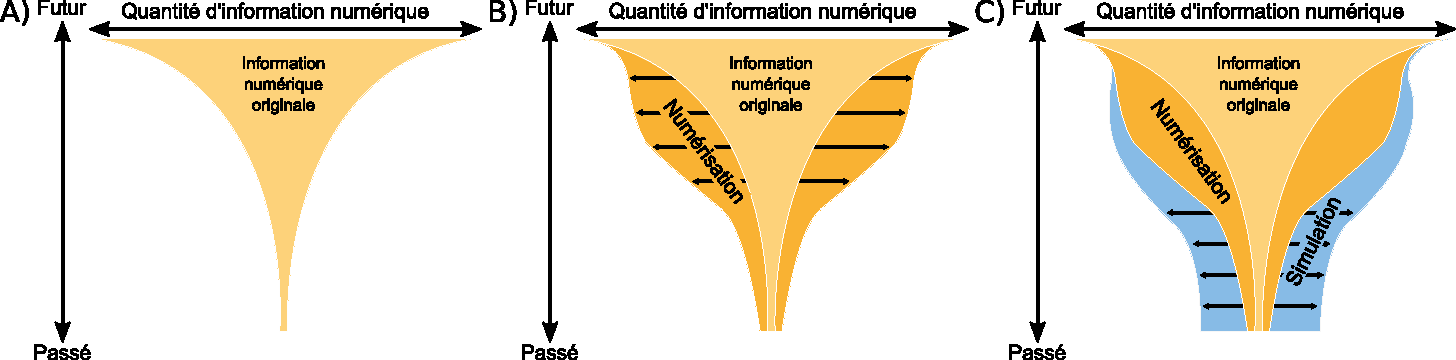
\includegraphics[width=\linewidth]{img/champignon_informationnel_kaplan.pdf}
	\caption{Le \og champignon informationnel\fg{} de \textcite{kaplan_lancement_2013}.}
	\label{fig:champignon-kaplan}
\end{figure}

L'exercice de la modélisation demande pourtant une quantité substantielle de données, et surtout que ces données soient homogènes en terme de couverture spatio-temporelle et en terme de certitude.
Afin d'augmenter la couverture spatio-temporelle, on a recours à des sources variées -- matérielles, écrites, voire biologiques --, par nature hétérogènes.

Les éléments empiriques ne peuvent dès lors reposer que sur une connaissance large et diversifiée des périodes et régions étudées.
Cette connaissance, que l'on peut qualifier d'experte, est l'apanage des \og thématiciens\fg{} du projet.
Le modélisateur, qui ne peut imaginer acquérir l'ensemble des connaissances expertes des thématiciens, doit accepter de leur faire entièrement confiance quant aux éléments empiriques mobilisés dans le modèle et par les biais desquels les modèles seront ensuite évalués.

Cela mène à une double implication en matière d'illégitimité.
Pour le modélisateur, cela implique qu'il sera toujours nécessaire de s'en remettre à la connaissance experte d'une personne (ou d'un groupe), sans possibilité d'ailleurs d'enrichir ces connaissances de son côté : mobiliser une référence scientifique dans une thématique de recherche inconnue ou distante, c'est risquer de citer des travaux non reconnus par la communauté, dépassés, ou encore anecdotiques.
Dans cette thèse, les tentations de référencer certains éléments empiriques en menant des recherches bibliographiques ont été nombreuses, mais sans vision d'ensemble de l'historiographie de ces sujets, cela n'ajouterait en fait aucun gage de scientificité.

Pour le thématicien, cela implique d'être en permanence \og malmené\fg{} par un modélisateur en recherche de connaissances plus précises et exhaustives.
Pierre \textsc{Garmy} le résume ainsi à propos de son expérience en tant que thématicien dans le projet TransMonDyn :
\begin{quotation}
\noindent \og La collaboration interdisciplinaire entre thématiciens et modélisateurs suppose le dépassement de deux contradictions : exhaustivité tendancielle \textit{vs} parcimonie recherchée d’une part et complexité \textit{vs} schématisation ou stylisation d’autre part.

\noindent Il existe un véritable paradoxe entre l’incomplétude de fait des données -- que les spécialistes disciplinaires cherchent à combler progressivement par l’enrichissement continu des corpus au moyen de recherches appropriées, rentabilisées par la définition de problématiques préalables aussi pointues que possible -- et l’attente des interlocuteurs modélisateurs qui veulent tout savoir et se bercent souvent d’illusions sur l’état de l’art réel dans chaque champ de connaissances. \fg{} \\
\mbox{}~ \textsc{Garmy} P., \og Annexe 1 - Retour sur expérience d’un “thématicien” \fg{}, in \textcite[476]{ouriachi_lelaboration_2017}  	  
\end{quotation}


\subsection{Dans un contexte fortement interdisciplinaire}


\section{Quel questionnement et évolution ?}

\subsection{Sujet initial}

\subsection{Verrous}

\subsection{Nouvelles questions}

\section{Quelle position ?}

\subsection{Co-construction}

\subsection{Interface}

\subsection{Démarche exploratoire}

\section*{Conclusion}
\addcontentsline{toc}{section}{\protect\numberline{}Conclusion}

%\setcounter{part}{0}
%\part{Accompagner la modélisation d'une transformation dans le système de peuplement de l'Europe médiévale}

\graphicspath{{chap2/}}
\setcounter{chapter}{1}
% !TEX root = ../These_Robin_Master.tex
\chapter{Formaliser connaissances et hypothèses, vers un modèle de simulation co-construit : SimFeodal}
\label{chap:chap2}
\begin{center}
	{\large Version \hl{2019-05-02}}
\end{center}

\begin{itemize}
	\item Avril 2019 : Nouveau départ pour le chapitre
\end{itemize}
\setcounter{minitocdepth}{1}

	\minitoc


\textbf{Code couleur}
\begin{itemize}
	\item Texte écrit pour cette version du chapitre
	\item {\redroman Texte publié dans le chapitre de Peupler la Terre}
	\item {\blueroman Modifications dans le texte du chapitre de Peupler la Terre}
\end{itemize}

\clearpage

\addcontentsline{toc}{section}{\textit{\textmd{Avant-propos}}}

\begin{mdframed}[backgroundcolor=gray!10,footnoteinside=false]
	\textbf{\hypertarget{avant-propos}{Avant-propos}}\vspace{-.75cm}
	\begin{multicols}{2}
Le présent chapitre décrit un modèle, SimFeodal, qui est une œuvre profondément collective et interdisciplinaire.
La paternité de ce modèle est ainsi à attribuer à l'auteur de ces lignes autant qu'à l'ensemble des co-concepteurs du modèle :
\begin{itemize}
	\item Cécile \textsc{Tannier}, UMR 6049 ThéMA -- Besançon\\
	Géographe et modélisatrice, Directrice de Recherche, CNRS
	\item Samuel \textsc{Leturcq}, UMR 7324 CITERES-LAT -- Tours\\
	Historien, Maître de Conférence, Université François Rabelais
	\item Élisabeth \textsc{Zadora-Rio}, UMR 7324 CITERES-LAT -- Tours\\
	Archéologue, Directrice de Recherche émérite, CNRS
\end{itemize}
Ainsi qu'à ceux qui ont contribué au projet pendant ses premières années :
\begin{itemize}
	\item Élisabeth \textsc{Lorans}, UMR 7324 CITERES-LAT -- Tours\\
	Archéologue, Professeure, Université François-Rabelais
	\item Xavier \textsc{Rodier}, UMR 7324 CITERES-LAT -- Tours\\
	Archéologue, Ingénieur de Recherche HDR, CNRS

\end{itemize}
Ce chapitre de thèse constitue une reprise, individuelle et largement modifiée et retravaillée, d'un chapitre -- \citetitle{cura_transition_2017} \autocite{cura_transition_2017} -- de l'ouvrage collectif \og Peupler la terre\fg{} \autocite{sanders2018peupler} issu du projet TransMonDyn\footnotemark.
Dans cette thèse, SimFeodal est présenté dans une version différente de celle de l'ouvrage collectif, et de nombreux mécanismes sont par exemple considérablement simplifiés.
Les fondements du modèle, toutefois, restent très largement identiques entre ces deux versions, et à ce titre, ce chapitre de thèse reprend parfois des passages entiers du chapitre de l'ouvrage collectif.
Dans ces moments, nous avons préféré ne pas les identifier en tant que tel, notamment car l'entremêlement de modifications apportées rendrait difficile la lecture.\\
En matière de forme, notons que contrairement au chapitre publié et aux parties traitant du modèle de l'Habilitation à Diriger des Recherches de Cécile \textsc{Tannier} \autocite{tannier_analyse_2017}, le modèle SimFeodal est ici présenté en suivant le protocole de description \og ODD\fg{} (\textit{Overview, Design concepts, and Details}) \autocite{grimm_odd_2010}, dans sa formulation la plus récente (\cite{grimm_documenting_2017}, voir \cref{tab:proto-ODD}).
SimFeodal ne se prête pas à toutes les catégories identifiées par les auteurs de ce standard, et celui-ci n'est de plus pas pensé pour une description aussi détaillée du modèle\footnotemark, mais nous pensons tout de même que le suivi de ce standard d'adoption permettra d'augmenter la reproductibilité de SimFeodal.
Pour cette même raison, notons que l'implémentation du modèle, son historique ainsi que les différentes descriptions techniques sont disponibles dans le dépôt de versionnement de SimFeodal :\\ \\
\footnotesize
\href{https://github.com/SimFeodal/SimFeodal}{https://github.com/SimFeodal/SimFeodal}

\end{multicols}

\end{mdframed}
\footnotetext[1]{
Projet ANR (ANR-10-BLAN-1805), coordonné par Lena \textsc{Sanders}, entre 2011 et 2014.
\href{www.transmondyn.parisgeo.cnrs.fr}{www.transmondyn.parisgeo.cnrs.fr}
}
\footnotetext[2]{
\hl{Une description plus courte, plus proche des descriptions ODD classiques, est disponible en ligne.}
}

\clearpage

\begin{table}[H]
	\centering
	\caption{Les éléments du protocole ODD, d'après \cite[Table 15.1, pp. 353--354]{grimm_documenting_2017}}
	\label{tab:proto-ODD}
	\scriptsize
	{\renewcommand{\arraystretch}{1.5}%
	\begin{tabular}{|p{1.05cm}|p{1.15cm}|p{1.25cm}|p{10cm}|}
		\hline
		\textbf{Overview} & \multicolumn{2}{l|}{1. Purpose} & What is the purpose of the model ? \\ \hline
		& \multicolumn{2}{l|}{\pbox[c][24pt][b]{3cm}{2. Entities, state variables, and scales}} & What kind of entities are in the model? Do they represent managers, voters, landowners, firms or something else? By what state variables (attributes or characteristics), are these entities characterized? What are the temporal and spatial resolutions and extents of the model? \\ \cline{2-4} 
		& \multicolumn{2}{l|}{\pbox[c][24pt][b]{3cm}{{3. Process overview and scheduling}}} & What entity does what, in what order?  When are state variables updated? How is time modeled: as discrete steps or as a continuum over which both continuous processes and discrete events can occur? \\ \cline{2-4} 
		\textbf{Design concepts} & 4. Design concepts & Basic principles & Which general concepts, theories or hypotheses are included in the model’s design? How were they taken into account? \\ \cline{3-4} 
		&  & Emergence & What key results are emerging from the adaptive traits, or behaviors of individuals? What results vary in complex/unpredictable ways when particular characteristics change? \\ \cline{3-4} 
		&  & Adaptation & What adaptive traits do the individuals have? What rules do they have for making decisions or changing behaviour in response to changes in themselves or their environment? Do agents seek to increase some measure of success or do they reproduce observed behaviours that they perceive as successful? \\ \cline{3-4} 
		&  & Objectives & If agents (or groups) are explicitly programmed to meet some objective, what exactly is that and how is it measured? When individuals make decisions by ranking alternatives, what criteria do they use? \\ \cline{3-4} 
		&  & Learning & May individuals change their adaptive traits over time as a consequence of their experience? If so, how? \\ \cline{3-4} 
		&  & Prediction & Prediction can be part of decision-making; if an agent’s learning procedures are based on estimating future consequences of decisions, how they do this? What internal models do agents use to estimate future conditions or consequences? What ‘tacit’ predictions are implied in these internal model’s assumptions? \\ \cline{3-4} 
		&  & Sensing & What aspects are individuals assumed to sense and consider? What aspects of which other entities can an individual perceive (e.g. displayed ‘signals’)? Is sensing local, through networks or global? Are the mechanisms by which agents obtain information modeled explicitly in a process or is it simply ‘known’? \\ \cline{3-4} 
		&  & Interaction & What kinds of interactions among agents are assumed? Are there direct interactions where individuals encounter and affect others, or are interactions indirect, e.g. via competition for a mediating resource? If the interactions involve communication, how are such communications represented? \\ \cline{3-4} 
		&  & Stochasticity & What processes are modeled by assuming they are random or partly random? Is stochasticity used, for example, to reproduce variability in processes for which it is unimportant to model the actual causes of the variability, or to cause model events or behaviours to occur with a specified frequency? \\ \cline{3-4} 
		&  & Collectives & Do the individuals form or belong to aggregations that affect, and are affected by, the individuals? Such collectives can be an important intermediate level of organization. How are collectives represented – as emergent properties of the individuals or as a separate kind of entity with its own state variables and traits? \\ \cline{3-4} 
		&  & Observation & What data are collected from the ABM for testing, understanding, and analyzing it, and how are they collected? \\ \hline
		\textbf{Details} & \multicolumn{2}{l|}{5. Initialisation} & What is the initial state of the model world, i.e., at time t = 0? How many entities of what type are there initially, and what are the values of their state variables (or how were they set)? Is initialization always the same, or is it varied? Are the initial values chosen arbitrarily or based on available data? \\ \hline
		& \multicolumn{2}{l|}{6. Input data} & Does the model use input from external sources such as data files or other models to represent processes that change over time ? \\ \cline{2-4} 
		& \multicolumn{2}{l|}{7. Submodels} & What are the submodels that represent the processes listed in ‘process overview and scheduling’ ? What are the model parameters, their dimensions, and reference values ? How were submodels designed or chosen, tested, and parameterised ? \\ \hline
	\end{tabular}}
\end{table}

\clearpage


\section*{Introduction}
\label{sec:chap2-intro}
\addcontentsline{toc}{section}{Introduction}

A rédiger :
- Modèle exploratoire -> KIDS + très évolutif + changements non linéaires/mono-directionnels


\section[Objectifs du modèle SimFeodal --  \textit{Purpose}]{Objectif du modèle SimFeodal\protect\newline \large{\textit{Purpose}}}


\subsection{Contexte historiographique}

{\redroman
	La question de l'émergence de la société féodale en Occident est au cœur d'un débat historique ancien.
	Depuis le XVIIIe siècle, les penseurs cherchent à comprendre le fonctionnement de la société médiévale et à cerner ses fondements.
	Les archives sont continûment explorées pour comprendre isolément et précisément les multiples facteurs à l'œuvre dans les processus qui ont fait émerger une société dite « féodale » dans le courant des Xe-XIe siècles.
	Cette compréhension se heurte toutefois à la très grande complexité de ces processus, qui peuvent varier chronologiquement, mais aussi présenter des nuances infinies en fonction des zones étudiées.
	Ces difficultés sont encore amplifiées par l'accès aux données, très variable selon l'état de la documentation, soumise aux aléas de la conservation ; d'une manière générale, les historiens des temps féodaux travaillent sur des documents rares et lacunaires, vestiges d'une société fondamentalement portée par l'oralité.
	
	Depuis une quarantaine d'années, l'afflux massif de données de fouilles issues du développement de l'archéologie préventive a permis de renouveler et enrichir ces débats.
	Les sources textuelles, qui apportent un éclairage plutôt normatif de la société, peuvent désormais être confrontées à des sources matérielles propres à mieux cerner les dimensions pratiques.
	Toutefois, cette complémentarité des approches textuelles et matérielles, loin de simplifier les questionnements portant sur la société féodale, les a encore complexifiés en mettant en évidence des aspects anthropologiques et des différenciations géographiques jusqu'alors sous-estimés.
	Le débat s'en est trouvé vivifié, se focalisant désormais sur la question de l'occupation de l'espace, considéré comme un marqueur efficace des transformations sociales.
	L'émiettement et la dissémination des pouvoirs, dont témoigne la multiplication des châteaux (seigneuries châtelaines), se font concomitamment à l'apparition d'un réseau très structuré d'encadrement religieux (paroissialisation de la société), tandis que se fixe de manière définitive un système de peuplement fondé sur un maillage villageois, cœur d'une vie communautaire active.
	
	C'est donc autour de l'articulation de ces trois éléments fondamentaux de la société féodale (châteaux, églises paroissiales, villages) que portent aujourd'hui analyses et théories.
	Fixation, polarisation et hiérarchisation des centres de peuplement sont désormais les grands processus sociaux examinés à la loupe pour aborder la société médiévale.
	Les historiens médiévistes analysent l'« encellulement » de la société \autocite{fossier_enfance_1982}, pistant d'une part les rôles polarisateurs du château (phénomène d'\textit{incastellamento},  \cite{toubert_les_1973}) et de l'église paroissiale accompagnée de son cimetière, considérés comme points de ralliement des populations paysannes, et d'autre part les manières dont les populations organisent collectivement les espaces de production (terroir villageois) pour assurer une répartition équilibrée des ressources.
	
	Dans ce contexte, la période 800-1100 est habituellement considérée comme une période de transition, durant laquelle la société féodale se structure, certains évoquant la « révolution de l'an Mil » \autocite{fossier_enfance_1982}, tandis que d'autres tempèrent en parlant de « révélation de l'an Mil » \autocite{barthelemy_societe_1993} (« révélation » par l'augmentation en quantité et en qualité de la documentation textuelle).
	Les hypothèses sont ainsi nombreuses, et il est difficile de trancher en faveur de l'une ou l'autre, tant l'articulation des facteurs sociaux, politiques, institutionnels, économiques et culturels est complexe.
}

\subsection{Questionnement}

{\redroman
	Dans le cadre de l'ANR TransMonDyn, l'objectif, pour la transition des années 800-1100, est d'étudier les processus à l'œuvre dans la dynamique de fixation, polarisation et hiérarchisation de l'habitat rural.
	L'approche est résolument géographique ; ce sont les implications spatiales des changements sociaux qui sont au cœur de l'étude.
	La modélisation ne porte pas sur les transformations politiques et sociales elles-mêmes, mais sur leur impact sur le système de peuplement.
	Le cœur du questionnement réside dans l'examen de la combinaison des facteurs ayant permis, entre 800 et 1100, la formation d'agrégats de foyers paysans dans une forme hiérarchisée et durable, polarisés par des châteaux ou des églises.
	Il s'agit d'analyser, par la modélisation et la simulation informatique, les conditions d'émergence du maillage villageois.
}


\section[Entités et échelles -- \textit{Entities, state variables, and scales}]{Entités et échelles\protect\newline \large{\textit{Entities, state variables, and scales}} \sectionmark{Entités et échelles}}

\subsection{Entités}

Dans le modèle SimFeodal, de nombreux types hétérogènes d'agents interagissent. Ces agents sont des implémentations informatiques des acteurs et entités identifiées dans le modèle conceptuel qui a donné lieu à SimFeodal (voir \textcite[Tableau 1, \ppno~309--310]{cura_transition_2017}).
Au cœur du modèle, on retrouve les \textbf{Foyers Paysans}. Ces agents mobiles répondent à des mécanismes d'agrégation et de migration en fonction de leurs niveaux de \textit{satisfactions}, sur les plans matériel, spirituel et en terme de protection face aux violences.
Les satisfactions sont mesurées respectivement en fonction des droits prélevés par des \textbf{Seigneurs} au sein de \textbf{Zones de Prélèvements} (satisfaction matérielle) ; en fonction de leur distance aux \textbf{églises paroissiales} les plus proches (satisfaction religieuse) ; et en fonction de leur distance aux \textbf{châteaux} -- construits par les \textbf{Seigneurs} -- les plus proches (satisfaction protection).
Un niveau de satisfaction trop faible pousse les Foyers Paysans à migrer, soit dans un rayon local soit de manière globale.
Lors de ces migrations, les Foyers Paysans sont attirés par des \textbf{Pôles}, ensembles composites d'\textbf{Attracteurs} (\textbf{châteaux}, \textbf{églises paroissiales} et \textbf{agrégats} de population) qui jouent un rôle de fixation de la population.
Plus l'attractivité de ces pôles est importante, plus grandes sont leur chance d'attirer suffisamment de Foyers Paysans pour que ces derniers forment des \textbf{Agrégats} de population, qui leur apporteront alors un surcroît de satisfaction et permettront de fixer les Foyers Paysans présents et d'en attirer de nouveaux pour faire émerger une hiérarchie dans le système de peuplement.
Le \cref{tab:agents-simfeodal} résume les propriétés et caractéristiques de ces différents types d'agents.


\begin{table}[H]
	\centering
		\caption{Les différents types d'agents de SimFeodal.\\
		$\upalpha$ : Il s'agit ici d'ordres de grandeur (les nombres pouvant varier fortement en fonction des simulations) du nombre d'agents de chaque type en fin de simulation.\\
		$\upbeta$ : Les agents sans emprise spatiale (---) ne sont pas localisés dans l'espace du modèle.\\
		$\upgamma$ : Les agents sans comportement actifs (---) n'agissent pas en tant que tel, mais peuvent servir de support pour les actions d'autres agents.}
	\label{tab:agents-simfeodal}
	\footnotesize
	{\renewcommand{\arraystretch}{1.5}%
	\begin{tabular}{|p{1.75cm}|M{1.75cm}|M{2cm}|M{2cm}|M{4cm}|}
		\hline
		\textbf{Agent} & \textbf{Sous-type} & \makecell{\textbf{Quantité$^\upalpha$}} & \textbf{Emprise spatiale$^\upbeta$} & \textbf{Comportements actifs$^\upgamma$} \\ \hline
		\multicolumn{2}{|c|}{Foyers Paysans} & \makecell{$\approx$ 4 000 à \\75 000} & Ponctuelle & Migrations \\ \hline
		\multirow{2}{*}{Seigneurs} & \makecell{Grands\\Seigneurs} & $\approx$ 2 & --- & \multirow{2}{*}{\makecell{Création de zones de\\prélèvement,\\collecte de droits,\\ construction de châteaux}} \\ \cline{2-4}
		& \makecell{Petits\\Seigneurs} & $\approx$ 200 & Ponctuelle &  \\ \hline
		\multirow{3}{*}{\makecell{Zones de\\ Prélèvement}} & Foncier & $\approx$ 75 & \multirow{3}{*}{Zonale} & \multirow{3}{*}{---} \\ \cline{2-3}
		& Haute-Justice & $\approx$ 50 &  &  \\ \cline{2-3}
		& Autres droits & $\approx$ 300 &  &  \\ \hline
		\multirow{2}{*}{Églises} & Église & $\approx$ 300 & \multirow{2}{*}{Ponctuelle} & \makecell{---} \\ \cline{2-3} \cline{5-5} 
		& Église paroissiale & $\approx$ 200 &  & \makecell{Création de paroisse\\ \textit{(type d'attracteur)}} \\ \hline
		\multicolumn{2}{|c|}{Paroisses} & $\approx$ 200 & Zonale & --- \\ \hline
		\multirow{2}{*}{Châteaux} & Petits Châteaux & $\approx$ 40 & \multirow{2}{*}{Ponctuelle} & \multirow{2}{*}{\makecell{---\\\textit{(type d'attracteur)}}} \\ \cline{2-3} 
		& Gros Châteaux & $\approx$ 10 &  & \\ \hline
		Agrégats &  & $\approx$ 200 & Zonale & \makecell{Création de communautés\\ \textit{(type d'attracteur)}} \\ \hline
		Pôles &  & $\approx$ 300 & Zonale & \makecell{Attire les Foyers Paysans \\  \textit{(composés d'attracteurs)}} \\ \hline
		\end{tabular}}
		\end{table}

\subsection{Échelles spatiales et temporelles}

\subsubsection{Résolution et échelle spatiale \label{subsec:reso-spatiale}}

SimFeodal prend appui sur un monde théorique \textbf{isotrope}, \textbf{continu}, symbolisé sous la forme d'un \textbf{carré de 80 km de côté}, strictement \textbf{endogène} au modèle.

\paragraph[Isotrope]{} Le monde est \textbf{isotrope} car il présente aucune hétérogénéité de surface ou de topologie : la distance entre deux points est mesurée de manière euclidienne.
Cet espace support se veut ainsi le plus neutre possible, proche d'un \og modèle nul\fg{}, susceptible de cette manière de représenter l'ensemble de la diversité des espaces de l'Europe du Nord-Ouest par l'entremise de ce dessin théorique.

\paragraph[Continu]{}Contrairement à un usage classique en simulation à base d'agents, nous avons aussi fait le choix de placer SimFeodal dans \textbf{un espace continu}, c'est-à-dire non discrétisé. La discrétisation de l'espace, sous forme de \og patchs\fg{} ou de \og cellules\fg{}, s'inscrit souvent dans l'héritage des modèles à base d'automates cellulaires. Les \textit{patchs} prennent d'ordinaire la forme d'agents : cela facilite l'attribution de caractéristiques, comme un certain niveau de ressource, une altitude, une population agrégée etc.
Dans le cas de SimFeodal, l'espace n'est qu'un support : il ne possède aucune caractéristique propre, et de par sa nature isotropique, n'est pas amené à différencier d'éventuelles cellules les unes des autres.
Une large part des mécanismes de SimFeodal s'appuie sur la prise en compte de distances entre agents, à partir de seuils dont les ordres de grandeurs peuvent être très variables (de la centaine de mètre à plus de 10 km).
Nous avons donc préféré conserver une marge de manœuvre élargie en ne procédant pas à une discrétisation de l'espace.

\paragraph[Dimension]{}L'espace est formalisé sous la forme d'\textbf{un carré de 80 km de côté}. Le choix du carré s'inscrit dans la volonté d'isotropie, et la dimension est proche de l'ordre de grandeur des diocèses médiévaux.
Dans des versions précédentes de SimFeodal, le carré avait un côté de 100 km, que nous avons choisi de réduire afin d'approcher de la superficie de la Touraine médiévale sur laquelle nous prenons appui pour le calibrage du modèle. La superficie du département d'Indre-et-Loire actuel, ou encore du diocèse de Tours, sont ainsi d'environ 6 000 km². En choisissant un espace support de 80 $\times$ 80 km de superficie (6 400 km²), on facilite ainsi l'estimation des densités et mesures d'écartements dans le modèle au regard des connaissances empiriques.
Notons enfin que si l'espace support est bien un carré de 80 km de côté, on en retranche en réalité une partie (1 km de chaque côté, voir \cref{fig:espace-simfeodal}) pour définir un espace utile, ou \og espace réduit\fg{}. On s'assure ainsi qu'aucune localisation ne soit située trop proche des limites de l'espace, ce qui pourrait avoir pour effet de produire des \og effets de bords\fg{}, aussi bien informatiques qu'en termes d'anomalies de voisinages.
L'espace réel, utilisable dans le modèle, est donc de 79 $\times$ 79 km, soit 6 084 km².

\begin{figure}[H]
	\centering
\begin{tikzpicture}[scale=.5]
\draw[] (0,0) -- (0,10) -- (10,10) -- (10,0) -- cycle;
\draw[|-|, very thin, dashed] (0, 10.5) -- node[above] {80 km (Espace du modèle)} (10, 10.5);
\draw[|-|, very thin, dashed] (-0.5, 0) -- node[above, rotate=90] {80 km} (-0.5, 10);

\draw[color=red!50, fill = red!10] (0.5, 0.5) -- (0.5, 9.5) -- (9.5, 9.5) -- (9.5, 0.5) -- cycle;
\draw[|-|, very thin, dashed, red!50] (10.50, 9.50) -- node[above, red!50, rotate=-90] {79 km} (10.5, 0.5);
\draw[|-|, very thin, dashed, red!50] (0.5, -0.5) -- node[below, red!50] {79km (Espace réduit)} (9.5, -0.5);
\end{tikzpicture}
\caption{L'espace support de SimFeodal, un monde théorique.\\
N.B : Dans le schéma, pour une question de lisibilité, les dimensions de l'espace réduit ne sont pas proportionnelles à celles de l'espace d'ensemble.}
\label{fig:espace-simfeodal}
\end{figure}

\paragraph[Endogène]{} Notons enfin que l'espace est strictement \textbf{endogène} au modèle. On entend par là que le monde n'est pas résultant du chargement d'un fichier géographique ou d'un paramétrage précis : seul un paramètre, qui régit la taille des côtés, joue sur la géométrie de l'espace.
Il nous semble important de le préciser, en particulier parce que c'est, à notre connaissance, assez inhabituel dans la simulation de données géographiques, mêmes théoriques : les agents sont placés de manière strictement aléatoire (via un aléa contrôlé tout de même) dans l'espace du modèle, et dès lors, aucune localisation ou surface ne sont identiques ou comparables d'une simulation à l'autre.


\subsubsection{Granularité temporelle}

SimFeodal modélise des processus qui se déroulent sur le temps long, et à ce titre, la gestion de la temporalité y est importante.
Le modèle inscrit son exécution dans une étendue de \textbf{400 ans}, \textbf{discrétisée} sous la forme de 20 pas de temps de \textbf{20 ans} chacun.

\paragraph[Durée]{} La période d'étude, thématique, s'étend entre 800 après J.-C. et 1100, qui correspondent à des repères temporels entre lesquels on estime que le plus gros de la transition étudiée s'est déroulée.
Pour modéliser ces évolutions, nous avons choisi de commencer à la même date, mais de prolonger l'exécution du modèle d'un siècle, portant donc l'intervalle modélisé à \textbf{400 ans}, \textbf{de 800 à 1200}\footnote{
	Dans les versions précédentes de SimFeodal, \textcite{cura_transition_2017} notamment, cette date était fixée à 1160. Nous avons choisi de prolonger de 40 ans parce que cela nous permet de comparer l'état final du modèle au début du XIII$^e$ siècle, et qu'on obtient ainsi un nombre de pas de temps plus \og rond\fg{} (20) qu'auparavant (18), ce qui permet par exemple de représenter l'évolution d'une simulation de manière plus régulière.
}. Prolonger cette date d'observation permet d'analyser le comportement du modèle après la période d'étude, et par exemple de voir si les processus à l'œuvre subissent bien un ralentissement, marquant par exemple la fin de la féodalité, plutôt qu'un accroissement constant.

\paragraph[Discret]{} Contrairement à la gestion de l'espace, nous avons choisi de modéliser le temps sous forme \textbf{discrète}.
On peut justifier ce choix avec deux raisons principales.
En premier lieu, la transition s'inscrit dans une forte incertitude temporelle. Les experts thématiques peuvent certes s'appuyer sur des dates précises, par exemple pour des années de réformes, mais les processus à l'œuvre s'inscrivent dans une durée floue, dont la résolution est difficilement réductible à moins d'un demi-siècle, et à peine meilleure pour des éléments matériels.
Avoir une vision continue du temps s'inscrirait ainsi dans une certaine sur-détermination du modèle en rapport aux connaissances thématiques sur lesquelles il s'appuie.
En second lieu, les processus sont modélisés à la résolution de \og foyers paysans\fg{}, c'est-à-dire à l'échelle de foyers plus que d'individus. Les migrations des foyers paysans correspondent empiriquement plutôt à des déplacements qui surviennent à l'échelle temporelle de la génération, c'est-à-dire que ces migrations se réalisent en fait quand les descendants d'un foyer s'établissent dans une nouvelle localisation.
La prise en compte d'un temps continu impliquerait donc la mise en place de bien plus de mécanismes probabilistiques, avec des aberrations potentielles plus importantes en terme de trajectoires des agents.

\paragraph[Pas de temps de 20 ans]{} Cette deuxième justification participe au choix de la granularité du modèle. \textbf{Les pas de temps ont une durée de 20 ans}, ce qui correspond à peu près à la durée d'une génération de l'époque.
Cela correspond aussi à la précision globale que l'on peut avoir sur l'apparition d'éléments matériels tels que les églises, paroisses et châteaux\footnote{
Certains de ces éléments sont connus avec une précision bien supérieure, par exemple quand des textes historiques mentionnent leur création. Ce n'est toutefois pas généralisé, et la granularité moyenne gravite donc plutôt autour de 20 à 40 ans.
}.
Dans l'ensemble, au vu des connaissances historiques, ces pas de temps doivent être interprétés comme des repères temporels plus que comme des dates précises. Que les premiers châteaux apparaissent en 980 ou en 1000 n'a pas d'importance dans le modèle, dans que cela se déroule avant la seconde moitié du XI$^e$ siècle par exemple.


La \cref{fig:frise-chrono} illustre les processus et événements qui surviennent pendant l'ensemble de cette période.

\begin{figure}[H]
	\centering
	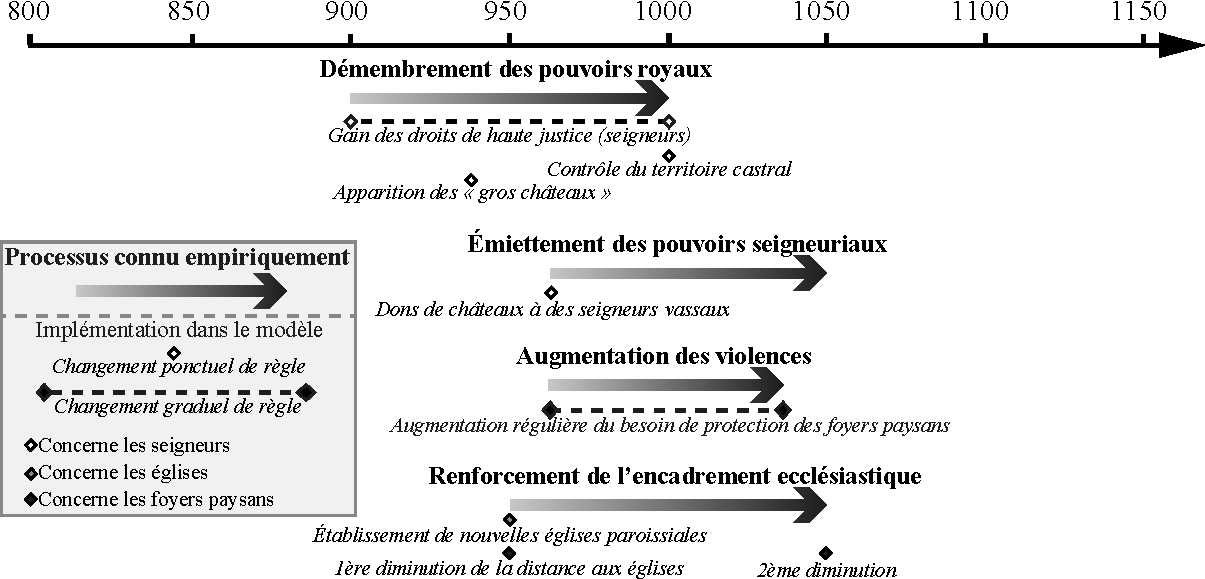
\includegraphics[width=\linewidth]{img/frise_chrono_tmd.pdf}
	\caption{Frise chronologique des processus historiques observés en Touraine implémentés dans SimFeodal. \hl{Figure issue de Peupler la Terre, à corriger/adapter.}}
	\label{fig:frise-chrono}
\end{figure}

\section[Fonctionnement général -- \textit{Process overview and schedulling}]{Fonctionnement général\protect\newline \large{\textit{Process overview and schedulling}} \sectionmark{Fonctionnement général} \label{sec:fonctionnement-general}}

SimFeodal est un modèle qui s'inscrit plutôt dans une approche KIDS que KISS (\hl{voir chapitre 1}).
Il est donc constitué d'une large variété d'agents (\cref{tab:agents-simfeodal}), dotés pour certains de nombreux comportements.
Au total, ce sont près de quarante mécanismes particuliers (ici regroupés en une quinzaine de mécanismes généraux), appelés selon un ordonnancement constant, qui font interagir les agents à chaque pas de temps.
Dans cette partie, nous présentons une synthèse de ces mécanismes, sans entrer dans le détail, algorithmique ou mathématique, de chacun (voir la \cref{sec:meca-specifiques} pour des descriptions plus précises des mécanismes les plus complexes et importants).

\subsection*{Ordonnancement général \label{meca-ordonancement}}

\begin{figure}[H]
	\centering
	% Couleurs
	\definecolor{bleuciel}{HTML}{a6cee3}
	\definecolor{mauve}{HTML}{1f78b4}
	\definecolor{beige}{HTML}{b2df8a}
	\definecolor{vert}{HTML}{33a02c}
	\definecolor{rose}{HTML}{fb9a99}
	\definecolor{rouge}{HTML}{e31a1c}
	% Styles des noeuds et lignes
	\tikzstyle{block} = [rectangle, draw, minimum width=4em, align=center, rounded corners, minimum height=2em, thick]
	\tikzstyle{start} = [draw, circle, minimum height=2em, align=center, thick]
	\tikzstyle{temp} = [very thick, dashed]
	\tikzstyle{line} = [draw, -{Latex[length=2.5mm,width=2.5mm]}]
	\tikzstyle{dline} = [draw, -{Latex[length=2.5mm,width=2.5mm,black!50]}, black!50, densely dotted]
	% 
	\tikzstyle{fps} = [fill=bleuciel]
	\tikzstyle{agregats} = [fill=mauve]    
	\tikzstyle{seigneurs} = [fill=vert]
	\tikzstyle{globals} = [fill=rouge!80]
	\tikzstyle{eglises} = [fill=rose!80]
	\tikzstyle{zps} = [fill=beige]
	\begin{tikzpicture}[node distance = .75cm and .75cm, auto, scale=0.7,every node/.style={transform shape}]
	% Place nodes
	\node [start, fill=rouge!80] (init) at (0,0) {Init.\\du\\monde};
	
	\node [start ,right= of init] (start) {Début\\du tour};
	\node [block, globals,right= of start] (maj-globals) {MaJ des \\variables\\globales};
	\node [block, fps, right= of maj-globals] (renouvellement-fp) {Renouvellement\\des FP};
	\node [block, eglises,right= of renouvellement-fp] (maj-paroisses) {Détection et\\promotions des\\paroisses};
	\node [block, agregats, right = of maj-paroisses] (maj-poles) {Détection\\des\\Pôles};
	
	\node [block, fps, below= of maj-poles] (maj-satisfaction) {MaJ satisfactions des FP};
	\node [block, fps, below=of maj-satisfaction] (migration-fp) {Migration des FP};
	\node [block, seigneurs, temp, below =of migration-fp] (maj-droits) {Gains de \\droits des seigneurs};
	\node [block, seigneurs, below=of maj-droits] (maj-zp) {Collecte des droits};
	
	\node [block, seigneurs, left=of maj-zp] (maj-dons) {Dons droits\\ et châteaux\\des Seigneurs};
	\node [block, globals, temp, left=of maj-dons] (promo-chateaux) {Promotion\\des châteaux};
	\node [block, seigneurs, temp, left=of promo-chateaux] (constructions-chateaux) {Construction\\ de châteaux};
	\node [block, seigneurs, left=of constructions-chateaux] (creation-seigneurs) {Création des\\nouveaux Seigneurs};		
	
	\node [block, agregats, above= of creation-seigneurs] (maj-agregats) {MaJ des Agrégats};
	\node [block, agregats, above=of maj-agregats] (maj-poles2) {MaJ des Pôles};
	\node [block, globals, above= of maj-poles2] (maj-outputs) {MaJ et enregistrement\\des \textit{outputs}};

	
	\path[line]%
	(maj-globals) -- (renouvellement-fp)
	(renouvellement-fp) -- (maj-paroisses)
	(maj-paroisses) -- (maj-poles)
	(maj-poles) -- (maj-satisfaction)
	(maj-satisfaction) -- (migration-fp)
	(migration-fp) -- (maj-droits)
	(maj-droits) -- (maj-zp)
	(maj-zp) -- (maj-dons)
	(maj-dons) -- (promo-chateaux)
	(promo-chateaux) -- (constructions-chateaux)
	(constructions-chateaux) -- (creation-seigneurs)
	(creation-seigneurs) -- (maj-agregats)
	(maj-agregats) -- (maj-poles2)
	(maj-poles2) -- (maj-outputs);

	
	\path[line] (init)-- (start);
	\path[line] (start) -- (maj-globals);
	\path[dline] (maj-outputs)-- (start);	
	\end{tikzpicture}
	\caption[a]{Ordonnancement des mécanismes de SimFeodal.\\
	{\footnotesize
	\colorbox{rouge!80}{\strut Mécanisme global} \colorbox{bleuciel}{\strut Foyers Paysans} \colorbox{rose!80}{\strut Églises} \colorbox{mauve}{\strut Agrégats et Pôles} \colorbox{vert}{\strut Seigneurs} \dbox{\strut Temporaire}
	}
	}
	\label{fig:ordonnancement}
\end{figure}

Dans SimFeodal, les mécanismes sont toujours appelés dans le même ordre (voir \cref{fig:ordonnancement}) : l'ensemble de l'ordonnancement ne change pas tout au long des 20 pas de temps du modèle.
Certains mécanismes sont toutefois temporaires, c'est-à-dire rendus inactifs en fonction des pas de temps : la construction des châteaux, par exemple, n'est pas possible avant 940.
Jusqu'au pas de temps correspondant, le mécanisme est donc désactivé par un paramètre réglable.
Notons que si les mécanismes suivent un ordre déterminé, ce n'est pas le cas des agents qui sont appelés dans chacun de ces mécanismes : pour un mécanisme donné, l'ordre d'appel des agents est aléatoire et varie à chaque appel de ce mécanisme.


\subsection{Initialisation \label{meca-init}}

L'initialisation du monde consiste à créer le monde théorique dans lequel les agents vont interagir et à générer ces derniers.
Pendant cette étape, des foyers paysans sont générés dans l'espace du modèle :  une très large proportion est instanciée de manière dispersée et aléatoire, et quelques dizaines d'agents sont localisés de manière agrégés afin de constituer les premiers agrégats de population, de tailles variables (une vingtaine de villages peu peuplés et quelques petites villes plus importantes, correspondant aux agglomérations secondaires antiques).
Lors de l'initialisation sont aussi créés les premiers seigneurs -- grands seigneurs sans portée spatiale et petits seigneurs localisés aléatoirement dans l'espace -- et les zones de prélèvement dans lesquelles ils prélèveront des droits divers.
L'initialisation est enfin l'occasion de créer et de disperser dans l'espace des églises (150), parmi lesquelles quelques-unes (50) se verront doter de droits paroissiaux et constitueront donc un premier maillage paroissial.

L'initialisation du monde est appelée une seule fois, avant que les pas de temps ne débutent. Elle repose fortement sur l'aléatoire, et génère donc une configuration spatiale différente à chaque nouvelle exécution du modèle (voir le paragraphe sur l'endogénéité de la \cref{subsec:reso-spatiale}).
Le détail de l'initialisation est décrit dans une partie ultérieure (\cref{sec:initialisation}), entièrement consacrée à cette étape préliminaire.

\subsection{Variables globales \label{meca-variables}}

Plusieurs mécanismes de SimFeodal dépendent du temps : la possibilité, évoquée plus haut, pour les seigneurs de construire un château, mais aussi, entre autre, l'évolution des distances que les foyers paysans sont prêts à parcourir pour se rendre à l'église, ce qui permet de formaliser l'impact des réformes grégoriennes.
La mise en place de mécanismes tributaires de dates nous permet ainsi de représenter des événements exogènes au modèle qui peuvent ainsi servir de déclencheurs ou de catalyseurs à des processus de longue durée.
L'incrémentation de la date et la mise à jour des différentes variables temporelles, par exemple en sélectionnant les valeurs de ces différentes variables dans des tableaux de correspondance temporels, constituent donc la première étape de chaque nouveau pas de temps.

\subsection{Renouvellement des foyers paysans \label{meca-renouvellement}}

SimFeodal est un modèle qui simule l'évolution d'un système spatial clôt.
On entend par là qu'il n'y a pas d'échange ou d'interaction avec les régions voisines, ce qui constitue une limite forte, par ailleurs fréquente dans la modélisation géographique.
Pourtant, en particulier dans un modèle mettant en place des migrations, il est difficile de s'abstraire du contexte spatial, le monde modélisé constituant certes un système en lui-même, mais aussi un système inscrit comme composante d'un système de peuplement plus large (le royaume des Francs, voire l'Europe du Nord-Ouest).
Nous avons donc choisi de modéliser les échanges avec l'extérieur par le biais d'un renouvellement partiel des foyers paysans.
A chaque pas de temps, une proportion (5\%) des foyers paysans existant est donc supprimée de la simulation, et une quantité équivalente est réinjectée dans l'espace du modèle.
Afin de ne pas bouleverser l'équilibre de l'agrégation, la localisation dans l'espace suit la proportion de foyers paysans dispersés et agrégés : s'il y avait 90\% de foyers paysans dispersés avant le renouvellent, 90\% des foyers paysans ré-injectés seront localisés aléatoirement dans l'espace du modèle, et les 10\% restant seront placés dans les agrégats existant\footnote{
Selon un tirage aléatoire pondéré : les agrégats les plus peuplés attireront potentiellement plus de ces nouveaux foyers paysans que les moins peuplés.
Cette logique d'attachement préférentiel (\hl{retrouver où j'en parle si c'est avant}) permet de modéliser l'attractivité qu'exercerait un agrégat peuplé, et donc potentiellement plus connu, sur des foyers paysans venant de régions voisines.
}.

\subsection{Mise à jour du maillage paroissial}

Le moyen-âge voit apparaître un maillage dense, continu dans l'espace, constitué autour d'églises dotées de droits paroissiaux : les paroisses, qui organisent l'ensemble de la vie spirituelle de la population.
Les archéologues ne s'accordent pas sur la date de leur apparition (avant la période étudiée), ni surtout sur le moment où elles constituent un maillage complet (vraisemblablement pendant la période modélisée), mais ils s'accordent sur le rôle de fixation et de stabilisation du territoire qu'elles ont eu \autocite{zadora-rio_paroisses_2008}.
Dans SimFeodal, cette étape de mise à jour du maillage paroissial regroupe en fait trois mécanismes distincts.

\paragraph{Dessin du maillage} Le maillage paroissial est représenté et calculé sous la forme d'une partition de Voronoï autour des églises paroissiales. On garantie ainsi un pavage complet du territoire, plus lâche dans les zones les moins peuplées et dotées de moins d'églises paroissiales, et plus dense dans les zones les plus peuplées, par exemple dans les agrégats les plus importants qui peuvent être déservis par de nombreuses paroisses ainsi qu'observé empiriquement.

\paragraph{Création de paroisses \og urbaines\fg{}} Dans les agrégats les plus peuplés, certaines paroisses peuvent être amenées à regrouper des centaines de paroissiens, ce qui ne correspondrait pas aux connaissances empiriques.
SimFeodal comprend donc un mécanisme de création de paroisses, donc de construction d'églises dotées de droits paroissiaux, au sein des agrégats les plus peuplés, selon une logique probabiliste : plus un agrégat est peuplé, plus il a de probabilités de voir apparaître une nouvelle église paroissiale, dans son étendue, dédiée à sa desserte.
Afin d'éviter l'apparition exponentielle d'églises paroissiales au sein d'un agrégat, cette probabilité est pondérée par le nombre d'églises paroissiales déjà présentes dans l'agrégat : là où un agrégat constitué de 1~000 foyers paysans et contenant une unique paroisse aura une probabilité de 50\% voir apparaitre une nouvelle églises paroissiale, un agrégat constitué de 1~000 foyers paysans mais déjà doté de 2 paroisses n'aura qu'une probabilité de 25\%.

\paragraph{Promotion de paroisses \og rurales\fg{}} Tout au long de son développement et à mesure de l'importance sociale qu'il acquière, on sait que le maillage paroissial se densifie, pour parvenir en fin de période au maillage quasi-communal qu'on lui connaît désormais. Cette densification est observée partiellement dans les zones denses, mais aussi très largement de manière homogène sur le territoire, notamment dans les zones les moins peuplées, afin de garantir un accès facilité aux sacrements à l'ensemble des foyers paysans.
Dans ces zones, on fait apparaître de nouvelles églises paroissiales, soit par promotion d'églises existantes (non dotées de droits paroissiaux), soit par construction de nouvelles églises qui deviendront centres paroissiaux.
Le mécanisme de ces créations est complexe, et on le détaille et l'illustre donc, à l'instar du détail des règles de création de paroisses \og urbaines\fg{}, dans la partie du chapitre relative aux spécificités des mécanismes (\cref{sssec:paroisses}).
Notons simplement que là encore, la promotion ou création d'églises paroissiales en zones peu denses suit une logique de seuil : si une paroisse contient trop de foyers paysans qui en sont suffisamment éloignés (donc que la paroisse a une très large superficie), on tendra à créer une nouvelle église paroissiale plus proche de ces foyers paysans.

\subsection{Détection des Pôles}

Dans SimFeodal, lorsque les foyers paysans migrent, ils sont attirés par des pôles, ensemble composites d'attracteurs (agrégats, églises paroissiales et châteaux), relativement à l'attractivité de ces pôles, c'est-à-dire au nombre et au type d'attracteurs qu'ils contiennent.
Les pôles sont donc indispensables au bon fonctionnement du mécanisme de migration, et leur définition revêt alors une importance nette.
Le mécanisme est encore une fois complexe (voir \cref{sssec:poles} pour le détail), mais on peut le résumer ainsi : un pôle est constitué par la proximité de plusieurs attracteurs, selon une logique de continuité spatiale.
Ainsi, quand une église paroissiale est située à proximité\footnote{
Cette proximité est configurable par le biais d'un paramètre.
Dans SimFeodal, on situe ce seuil à 200 mètres.
} d'un château, lui-même par exemple à proximité d'un agrégat de population, on définit un pôle comme composé par ces trois éléments, et représenté par l'enveloppe convexe formée par leurs géométries.
Afin de ne pas artificiellement diviser des pôles pré-existants, ou au contraire de voir apparaître de nombreux pôles dans un espace restreint (attracteurs séparés de 210 mètres par exemple), on procède ensuite à une fusion des pôles les plus proches, en considérant par exemple qu'un agrégat, quelle que soit son importance, contient et fait partie d'un seul pôle.

Les valeurs d'attractivité des pôles, relatives à leur composition en attracteurs, ont donné lieu à un important travail de paramétrage (\hl{voir chapitre 4, et particulièrement les étapes $n$--$j$}), et est désormais fixée selon ces principes (\cref{tab:attraction-poles}) :

\begin{table}[H]
	\centering
		\caption{Attractivité ($\in [0,1]$) conférée aux pôles par leurs attracteurs.}
	\label{tab:attraction-poles}
	{\renewcommand{\arraystretch}{1.1}%
	\begin{tabular}{|l|l|l|}\hline
		\textbf{Attracteur} & \textbf{Détail} & \textbf{Attractivité} \\ \hline
		\multirow{2}{*}{Châteaux} & Petit & 0.15 \\
		& Gros & 0.25 \\ \hline
		\multirow{4}{*}{Église paroissiale} & 1 & 0.15 \\
		& 2 & 0.25 \\
		& 3 & 0.5 \\
		& 4+ & 0.6 \\ \hline
		\multicolumn{2}{|l|}{Agrégat (doté d'une communauté)} & 0.15 \\ \hline
	\end{tabular}}

\end{table}

\subsection{Satisfaction des Foyers Paysans}

La satisfaction\footnote{
Notons que ce terme n'est pas entièrement \og satisfaisant\fg{} : la migration des foyers paysans est favorisée par une faible satisfaction, c'est-à-dire une absence de satisfaction (qui n'est donc pas un mécontentement ou \og insatisfaction\fg{}), dont l'on retrouve le sens dans le terme anglais \textit{dissatisfaction}.
} des foyers paysans est la condition préalable au mécanisme le plus important de SimFeodal, la migration.
Elle qualifie la capacité des foyers paysans à remplir leurs besoins fondamentaux : \og se nourrir\fg{} (satisfaction matérielle), \og assurer son salut\fg{} (satisfaction religieuse) et \og éviter d'être l'objet de violences\fg{} (satisfaction \og protection\fg{}) \autocite[Tableau 1, \ppno~309]{cura_transition_2017}.
La satisfaction d'ensemble, qui intervient dans la probabilité de migration, est donc une synthèse numérique de ces trois satisfactions spécifiques.
Ces composantes ne sont pas hiérarchisées, sinon en considérant qu'elles sont normalisées \og par le bas\fg{} : le satisfaction d'ensemble est égale à la plus faible de ses trois composantes, pondérée par l'appartenance à une communauté, laquelle procure un contre-pouvoir face aux différentes pressions subies par les foyers paysans.

Le détail des calculs est donnée dans la partie dédiée (\cref{sssec:satisfaction}), mais on peut toutefois déjà expliciter les choix de modélisation de chacune des composantes de la satisfaction d'ensemble.

\paragraph{Satisfaction matérielle}

Dans SimFeodal, on considère la satisfaction matérielle comme une fonction des différentes redevances dont un foyer paysan doit s'acquitter : plus il doit régler de droits, moins il est satisfait.
Comme pour la satisfaction générale, notons que l'appartenance ou non à une communauté intervient dans ce calcul : on estime en effet que les communautés (paysannes, rurales, villageoises\ldots) permettent de constituer une force suffisante pour exercer un véritable contre-pouvoir face à des seigneurs qui seraient trop exigeants.

\paragraph{Satisfaction religieuse}

La satisfaction religieuse représente la capacité d'un foyer paysan à se rendre facilement à l'église pour y assister aux différents sacrements (baptêmes, mariages, eucharistie\ldots) qui rythment la vie spirituelle de l'époque.
Dans SimFeodal, cette capacité est modélisée comme une fonction de la distance à l'église paroissiale la plus proche : plus on est éloigné d'une église paroissiale, plus la satisfaction est faible.
Les seuils de distance définissant le \og loin\fg{} et le \og proche\fg{} évoluent au cours du temps, afin de représenter l'alourdissement des obligations religieuses tout au long de la période, par exemple à l'occasion des réformes grégoriennes.

\paragraph{Satisfaction de \og protection\fg{}}

Avec la diminution du pouvoir de l'autorité centrale carolingienne assortie d'un émiettement des pouvoirs locaux, la région d'étude subit un regain de violences militaires dont l'un des symptômes représentatifs est l'apparition des châteaux forts.
De la même manière que la satisfaction religieuse dépend de la distance aux églises, on considère dans SimFeodal que la satisfaction \og protection\fg{} des foyers paysans dépend de la distance au château le plus proche.
Un château assure ainsi une certaine protection à la population, protection qui se montre de plus en plus critique au fur et à mesure de l'avancement de la période et donc du modèle.
Comme pour la satisfaction religieuse, les seuils de distance évoluent donc au cours du temps, de même ici que le \og besoin de protection\fg{}, qui permet de renforcer l'augmentation nette du climat de violence au cours de la période.

\subsection{Migration des Foyers Paysans \label{meca-migration}}

La satisfaction, décrit ci dessus, sert de condition probabiliste à la possibilité pour les foyers paysans de migrer.
Rappelons que les pas de temps durent 20 ans : les migrations ne sont donc pas des déplacements quotidiens ou saisonniers, mais illustrent plutôt le déménagement et le choix de localisation que chaque nouvelle génération de paysans est amené à réaliser.
Dans SimFeodal, nous considérons que les foyers paysans suffisamment satisfaits ne sont pas amenés à migrer : on migre quand on est insatisfait, et l'on cherche alors à augmenter sa satisfaction.
L'implémentation de cette logique suit un mécanisme probabiliste, où l'insatisfaction augmente la probabilité de migrer.
Le détail du mécanisme de migration est complexe et sera détaillé dans la \cref{sssec:migration}.
Notons aussi que ce mécanisme est sans doute le plus important et impactant du modèle SimFeodal : à ce titre, il a subit de très nombreux changements depuis le début de la conception du modèle, tel qu'illustré dans \hl{le chapitre 4}.

Dans la version actuelle de SimFeodal (version 6.3 présentée dans ce chapitre), la migration répond à une succession de conditions.
Dans l'ensemble, quand les foyers paysans migrent, c'est nécessairement vers un pôle, et si possible un pôle plus attractif que celui dans lequel ils seraient.
Cette migration peut prendre deux formes :
\begin{itemize}
	\item une migration \og locale\fg{}, où les foyers paysans cherchent des pôles plus attractifs dans un rayon défini (2~500 mètres) ;
	\item et la migration \og lointaine\fg{}, où au contraire les foyers paysans cherchent un agrégat\footnote{
		\textit{N.B.} : La migration locale se fait en direction d'un pôle (qui peut ou non contenir un agrégat), alors que la migration lointaine vise un agrégat, potentiellement plus important.
	} situé au delà du rayon local.
\end{itemize} 
La migration locale est privilégiée sur la migration lointaine, qui, en simplifiant, ne s'exerce que quand la première n'est pas possible (absence de pôles locaux, tirages de probabilité échoués etc.).

Notons que ces règles ne s'appliquent pas à l'identique à tous les foyers paysans : une part de ceux-ci (20\%), intitulés \og non mobiles\fg{}, n'ont pas la possibilité d'effectuer des migrations lointaines : ils sont restreints à des migrations locales, ce qui permet de modéliser le comportement de dépendances de certaines catégories de population historiques (les serfs et esclaves, qui n'avaient pas le droit de quitter le domaine de leur seigneur, par exemple).


\subsection{Gains de droits}

Au fur et mesure de l'avancement de la période, le pouvoir central s'efface et les ressorts locaux subissent un émiettement important, voyant apparaître de nombreux seigneurs de moindre importance (les chevaliers notamment).
Ces seigneurs gagnent et s'arrogent le prélèvement de nouveaux droits (droits banaux, droits de basse justice etc.), augmentant d'autant la charge fiscale dont doivent s'acquitter les foyers paysans.

Dans SimFeodal, cela est modélisé sous la forme de l'apparition constante de nouvelles zones de prélèvement par l'intermédiaire desquelles les seigneurs pourront prélever de nouveaux droits.
Cela peut concerner de nouveaux seigneurs, lors de leur apparition dans l'espace du modèle, ou au contraire se faire au bénéfice de seigneurs plus anciens.
Du point de vue de l'implémentation, ce comportement est formalisé sous la forme d'une probabilité ($0.15$), pour les petits seigneurs, de créer une nouvelle zone de prélèvement autour de leur localisation, à chaque pas de temps.

Ce mécanisme s'associe à une autre, majoritairement exercé par les grands seigneurs, qui leur permet de prélever, à partir d'une date donnée (voir \cref{meca-variables}), des droits de haute justice, là encore à partir d'un tirage de probabilité ($P = 0.2$ pour les grands seigneurs de 900 à 1000 et $1$ après; $P = 0.2$ pour les petits seigneurs châtelains à partir de 1000).

\subsection{Collecte des droits}

Dans SimFeodal, les droits sont prélevés au travers de représentations géographiques de leur emprise spatiale\footnote{
Notons bien qu'il s'agit d'un choix de modélisation, c'est-à-dire ici d'une simplification forte.
Les droits au moyen âge n'avaient pas nécessairement de logique spatiale : ce pouvait être en fonction de l'usage d'un matériel (four banal, moulin\ldots), ou en fonction d'une appartenance familiale (la \og taille\fg{} personnelle) par exemple, sans que la localisation précise n'entre en jeu.
} : les zones de prélèvement.
Celles-ci sont de trois types (cf. \cref{tab:agents-simfeodal}), qui correspondent à trois grandes catégories de droits connus : les droits fonciers ; les droits de haute justice ; et les autres droits, qui regroupent une forte diversité de redevances locales (droits banaux, droits de basse et moyenne justice, droits locaux\ldots).

Dans SimFeodal, chaque droit a ses propres modalités de collecte (voir le détail en \cref{sssec:collecte-droits}), mais on peut résumer cela de manière géométrique : les zones de prélèvement sont des cercles de rayon variables, qui se superposent et s'intersectent très largement.
Chacune de ces zones de prélèvement appartient à un seigneur, qui l'a créée, et peut en plus être confiée en garde à un autre seigneur (voir le paragraphe suivant).
Les seigneurs (propriétaires et gardiens) prélèvent des droits aux foyers paysans situés dans les zones de prélèvement.
Plus ces derniers sont situés dans une région dense en zones de prélèvements, plus ils seront amenés à s'acquitter de nombreux droits, et plus leur satisfaction matérielle sera faible.
Pour les seigneurs, à l'inverse, plus les redevances collectées seront importantes (donc plus ils posséderont de zone de prélèvement recouvrant de nombreux foyers paysans), plus leur puissance sera importante, ce qui leur permettra notamment de construire des châteaux, gages de renommée et de revenus accrus.

\subsection{Dons entre seigneurs \label{meca-dons}}

On a mentionné que les seigneurs pouvaient se voir confier des zones de prélèvement en garde.
Historiquement, cela correspond à la pratique de certains seigneurs de nommer des gestionnaires ou de distribuer des terres à des seigneurs de moindre importance pour s'assurer de leur vassalité.

Dans SimFeodal, les seigneurs peuvent donner en gardiennage, selon une probabilité, chacune de leurs possessions : zones de prélèvement et châteaux.
Dans le premier cas, les seigneurs récipiendaires sont choisis de manière privilégiée dans le voisinage des seigneurs donateurs : on favorise ainsi une transmission locale.
Pour les châteaux, il n'y a pas de préférence locale, mais seuls des seigneurs de faible importance peuvent être récipiendaires, c'est-à-dire ceux qui ne sont pas déjà châtelains (ie. qui n'ont pas déjà de château en propre ou en garde).

En donnant en garde leurs propriétés, les seigneurs se garantissent la constitution d'un réseau de vassalité (non modélisé) et accroissent leur puissance symbolique.
Dans SimFeodal, on le modélise en augmentant les redevances que les seigneurs collectent dans les zones de prélèvement données en gardiennage : le seigneur gardien collecte les redevances classiques, alors que le seigneur suzerain collecte ces mêmes redevances accrues d'un léger facteur\footnote{
Par exemple, un seigneur collecte une puissance (symbolique) de $1$ sur les foyers paysans dont il collecte les droits fonciers.
En nommant un \og gardien\fg{}, il y collectera $1.25$ de puissance, et le vassal récupèrera lui $1$.
}.
Notons que ces dons n'ont pas d'influence sur la satisfaction des foyers paysans : pour eux, seul un seigneur (le gardien, ou le propriétaire quand la zone n'a pas été confiée en gade) prélève les droits.
Le mécanisme de collecte n'est donc pas symétrique : les seigneurs y gagnent plus que ce que les foyers paysans n'y \og perdent\fg{}.

\subsection{Promotion des châteaux}

De nombreux châteaux ont été construits pendant la période étudiée.
Il y avait naturellement une forte hétérogénéité dans leur ampleur, leur importance stratégique et le degré de protection qu'ils apportaient.

Dans SimFeodal, on a choisi de simplifier cette hiérarchie en distinguant deux types de châteaux : les \og petits châteaux\fg{} et les \og gros châteaux\fg{}.
Les gros châteaux ont un pouvoir d'attraction plus développé (cf. \cref{tab:attraction-poles}), renforçant donc l'attraction des pôles qu'ils constituent et par là même accroissant la probabilité de voir se développer à proximité des agrégats majeurs.
Lors de leur création (voir \textit{infra}), les châteaux sont toujours des \og petits châteaux\fg{}.
Le mécanisme de promotion, probabiliste, permet à un château situé dans un pôle important (c'est-à-dire constitué de plusieurs attracteurs : agrégat, églises paroissiales) de devenir \og gros château\fg{}, et renforce donc l'attrait de ce pôle déjà avantageux.

\subsection{Construction de châteaux}

Tout au long de la période, de nouveaux châteaux sont construits et renforcés. C'est l'apparition des \og châteaux forts\fg{}.
Si l'on connaît des châteaux préalables à la période étudiée, leur démultiplication survient surtout à partir de la seconde moitié du X$^e$ siècle.
Ils sont surtout construits par les grands seigneurs existants afin de mailler le territoire d'un réseau de protection, même si certains sont aussi l'œuvre de seigneurs de moindre envergure qui se sont enrichis pendant la période en profitant du système féodal.
En Touraine, on considère que la majeure partie des châteaux forts ont été construits entre le X$^e$ et le XIII$^e$ siècle, et que leur production a ensuite fortement ralenti.
Les châteaux sont bâtis en bonne partie dans des villes déjà attractives, même si l'on observe aussi quelques créations dans des espaces peu peuplés, qui tendront alors à le devenir par la suite (les bourgs castraux).


Dans SimFeodal, on fait apparaître les châteaux de manière endogène, en considérant donc qu'il n'y en a aucun au début de la période.
À partir de 940, les seigneurs ont la possibilité de créer des châteaux.
Cette possibilité est basée sur une probabilité, fonction de la puissance des seigneurs, donc de l'accumulation des redevances perçues à chaque pas de temps.
Plus la puissance d'un seigneur est importante, plus il a de chances de pouvoir créer un château.
Cette probabilité est aussi fonction de la puissance relative des seigneurs : au fur et à mesure que le temps passe et que de nouveaux seigneurs émergent, les grands seigneurs historiques voient leur importance relative décliner, et donc leur probabilité de créer de nouveaux châteaux diminuer.
A contrario, certains petits seigneurs favorisés par leurs prélèvements et par les gardiennages reçus peuvent, de manière exceptionnelle, être amenés à bâtir eux-aussi des châteaux.
Afin de ne pas voir l'apparition de zones concentrant de nombreux châteaux, nous avons mis en place une restriction spatiale à leur implantation : un nouveau château ne peut être construit à moins de 5 km d'un château existant.
On garanti ainsi une répartition spatiale non aberrante au regard des connaissances empiriques.

Notons qu'en matière d'ordonnancement, la construction des châteaux a lieu après le calcul de la satisfaction protection des foyers paysans, de la promotion en gros châteaux, et aussi après le don de ces mêmes châteaux, ce qui pourrait sembler contre-intuitif.
Ce choix a été fait pour symboliser la durée de construction des châteaux, bien plus longue que les autres phénomènes d'apparition décrits dans le modèle : un château apparaît en fin de tour, il n'est donc pas véritablement utilisable avant le tour suivant, soit 20 ans plus tard.
Les détails du mécanisme, notamment en ce qui concerne les probabilités différentes pour les petits et les grands seigneurs, ou encore les choix de localisation des nouveaux châteaux (au sein d'un agrégat ou non par exemple), sont explicités dans la partie dédiée (\cref{sssec:constru-chateaux}).

\subsection{Création de nouveaux seigneurs}

L'émiettement des pouvoirs pousse à l'apparition de nombreux seigneurs, d'envergure très locale majoritairement, tout au long de la période : alors qu'on estime qu'il y avait une vingtaine de seigneurs en Touraine en début de période, on considère qu'il y en a plus de 200 en 1200.
Ces seigneurs sont détenteurs d'un faible pouvoir, peu disposant de terres conséquentes : une large proportion tire ses revenus de terres et d'installations octroyées par leur suzerain, par exemple sous la forme de banalités.

Dans SimFeodal, l'accroissement des seigneurs est modélisé sous la forme de l'apparition, à chaque pas de temps, d'un nombre légèrement aléatoire de nouveaux seigneurs, dont la variation est mesurée de manière à obtenir environ 200 seigneurs en fin de simulation.
Parmi ces seigneurs, seule une faible proportion (10\%) est dotée de terres et collecte donc des droits fonciers. Les autres seigneurs constituent donc un vivier potentiel de récipiendaires de dons divers (voir \cref{meca-dons}).
L'ensemble de ces seigneurs sont répartis, spatialement, au sein d'agrégats existants.

\subsection{Détection des agrégats \label{meca-agregats}}

L'un des constats forts ayant mené à l'identification d'une \og transition\fg{} \autocite{pumain_convergences_2017, nuninger_cadre_2017} dans le système de peuplement de l'Europe du Nord-Ouest est la hiérarchisation du système de peuplement, c'est-à-dire d'une part une concentration de la population dispersée, et d'autre part l'apparition de hameaux, villages et petites villes suivant une hiérarchie de population.
Parce que l'utilisation de ces termes plus spécifiques est particulièrement sensible en histoire et en archéologie, en particulier en raison de potentiels anachronismes, nous avons choisi de ne pas discrétiser le continuum représentatif de l'agglomération de foyers et de le dénommer, dans son sens le plus littéral, \og agrégat\fg{} de population.

Dans SimFeodal, ces agrégats sont interprétés de manière morphologique, à l'instar des agglomérations de l'INSEE : est agrégat un regroupement d'au moins 5 foyers paysans, espacés l'un à un autre d'au plus 100 mètres.
Cette définition permet de représenter des entités géographiques très diverses, depuis le petit agrégat composé de quelques foyers paysans à l'agrégat majeur, semblable à une petite ville, constitué de plusieurs centaines de foyers.
L'agrégat est une entité spatiale au sens propre, dotée par exemple de ses propres attributs et sa propre emprise spatiale, constituée par l'enveloppe convexe des foyers paysans qui le composent : c'est une entité individuelle mais composite.

Certains agrégats peuvent contenir une \og communauté\fg{}, c'est-à-dire une structure institutionnalisée gérée par les foyers la composant et qui procure un avantage en matière de rapport de force et de subsistance matérielle (par exemple avec les logiques de gestion collective des terres et outils que permettent les communautés agraires).
Dans SimFeodal, les agrégats ont une probabilité (20\%), à chaque pas de temps, de voir apparaître une communauté en leur sein.
D'un point de vue informatique, cela complexifie énormément la détection des agrégats : dès lors que des agents ont des propriétés propres, celles-ci doivent être transmissibles dans le temps, c'est-à-dire d'un pas de temps à l'autre.
Pourtant, la détection des agrégats est renouvelée à chaque pas de temps, ce qui signifie qu'un agrégat détecté en 900, situé au même endroit qu'un agrégat de 880, ne peut que difficilement lui être associé\footnote{C'est un problème récurrent des méthodes de \textit{clustering} dynamique que de réussir à mener des associations entre les \textit{cluster} de différentes dates.}.
Le mécanisme spécifique de détection, de constitution et de transmission des attributs des agrégats est donc particulièrement complexe, et fait l'objet d'une présentation détaillée plus loin dans le chapitre (\cref{sssec:agregats}).

\subsection{Actualisation des pôles}

La détection des pôles intervient relativement tôt dans l'ordonnancement des mécanismes.
Il est par exemple nécessaire que les pôles soient définis avant le mécanisme de migration des foyers paysans, qui dépend en partie de ces pôles.
Pourtant, en vue de préparer et de sauvegarder les \textit{outputs}, il est nécessaire de redéfinir les pôles, qui ont notamment été affectés par les modifications dans les agrégats et châteaux.
Cela permet par exemple, lors de l'enregistrement des sorties, de conserver un lien entre un agrégat et le pôle dans lequel il se situe, notamment pour étudier les relations entre composition des pôles et populations des agrégats qui y sont attachés.
Dans SimFeodal, nous sommes donc obligés, afin d'avoir des sorties exploitables, de reconstruire les pôles en fin de tour.
Cette duplication d'un mécanisme est malheureuse et peu optimale, mais rendue nécessaire par la structure des différents mécanismes précédents et en particulier par l'interdépendance qui caractérise de nombreux types d'agents dans le modèle.

\subsection{Enregistrement des \textit{outputs} \label{meca-outputs}}

Lors de la conception et du développement de SimFeodal, on a rapidement choisi de mener l'exploration du modèle très largement \textit{a posteriori} (\hl{voir chapitre 5, section 5.2.1}) de l'exécution du modèle.
L'enregistrement des données d'un modèle est un problème complexe, dont les enjeux et difficultés sont largement résumées dans le chapitre 5 (\hl{section 5.1}).
Notons ici, tout de même, que nous avons besoin d'enregistrer des données relatives à l'ensemble des agents, pris individuellement, et à leurs attributs.
La masse de données écrite par la simulation est donc assez conséquente et revêt une importance particulière.
Lors de cette phase, des variables globales et spécifiques sont actualisées, des indicateurs synthétiques sont calculés, et l'ensemble des données subit des traitements voués à en simplifier la conservation, par exemple en réduisant la précision des nombres décimaux\footnote{
Pour illustrer l'importance de ce traitement d'apparence anecdotique, on peut prendre l'exemple de l'enregistrement des géométries.
Celles-ci, dans la plate-forme Gama \autocite{taillandier_building_2018} utilisée pour SimFeodal, sont exportées dans un format textuel normalisé, le \og Well-Known Text\fg{} (\textit{WKT}).
Par défaut, chaque géométrie est décrite avec une précision de 12 chiffres décimaux, soit une résolution spatiale proche du picomètre, l'ordre de grandeur des atomes.
Cette précision n'a strictement aucune utilité dans un modèle où les ordres de grandeur minimums tournent autour des dizaines et centaines de mètres.
D'un point de vue informatique, stocker 12 décimales au lieu d'entiers démultiplie considérablement la place nécessaire pour l'enregistrement des données, et ces étapes de simplification sont donc indispensables pour disposer d'un modèle fonctionnel et exploitable.
}.

\section[Concepts de modélisation-- \textit{Design concepts}]{Concepts de modélisation \protect\newline \large{\textit{Design concepts}} \sectionmark{Concepts de modélisation}}

Cette section du protocole ODD vise à mettre en avant les concepts courants de la modélisation de systèmes complexes qui sont employés dans le modèle.
C'est une liste exhaustive, et l'ensemble des concepts décrits n'ont pas nécessairement de correspondance dans SimFeodal.
Par soucis de clarté, on décrira donc d'abord les grands principes de modélisation qui nous semblent fondamentaux dans SimFeodal, et ensuite, le cas échéant, les ensembles de concepts mobilisés.

\subsection{Principes de base - \textit{Basic principles}}

\paragraph{\textit{Space Matters}}

SimFeodal est un modèle intrinsèquement spatial.
De nombreux modèles agents mobilisent l'espace, ou au moins une représentation ou un support présent dans le concept du \og monde\fg{} virtuel répandu en modélisation agent, quand bien même l'approche n'est pas foncièrement spatiale.
Par exemple, on trouve de nombreux modèles de réseaux dans les bibliothèques classiques de modèles agents, où l'espace support est une vue planaire plus qu'un support euclidien ou topographique réel.\\
Dans SimFeodal, au contraire et comme la brève description des mécanismes le montre, une très large partie des (inter)actions dépendent des distances (modèles de types gravitaires pour le calcul de la satisfaction religieuse et de protection), des contextes spatiaux (évaluation de l'environnement local pour les migrations locales) ou encore des voisinages (constitution d'agrégats, détection des pôles etc.).
SimFeodal n'est donc pas qu'un modèle qui prend appui sur l'espace, mais un modèle dont le fonctionnement inhérent est spatial, voir géographique ou géométrique.
\textit{Space matters}\ldots

\paragraph{\textit{Push-Pull}}

L'évolution de la structure spatiale que l'on observe dans SimFeodal résulte de la migration des foyers paysans, qui tendent ainsi à se concentrer.
Ce mécanisme est fortement inspiré et ancré dans une certaine pratique de modélisation, courante dans le champ des études de mobilité résidentielle, que l'on peut qualifier de \og \textit{push-pull}\fg{} \autocite{tannier_analyse_2017}.
On entend par là que les agents subissent un double mécanisme, répulsif, qui les pousse à déménager (ou migrer dans SimFeodal), le \textit{push}, et attractif, qui conditionne leur choix de destination à l'attractivité d'un lieu, le \textit{pull}.
Ce modèle est d'ordinaire mobilisé dans l'étude de mobilités résidentielle, ou encore vis-à-vis de pratiques quotidiennes de l'espace, et nous semble inédit sur des processus d'une temporalité plus importante, telle que le temps long sur lequel SimFeodal s'appuie.\\
Si ce choix peut paraître surprenant, il résulte avant tout d'une certaine \og culture de modélisation\fg{}, l'une des co-conceptrices du modèle ayant une forte habitude de modélisation de dynamiques résidentielles (\textit{ibid.}).
En dehors de l'importance de cette \og path-dependency\fg{} d'un modèle aux conceptions préalables de ses modélisateurs, notons tout de même que ce type de modélisation nous semble assez facilitateur de dialogue avec des experts thématiques, permettant donc peut-être plus simplement que d'autres paradigmes de passer d'une connaissance experte spécifique à une modélisation plus générique.

\paragraph{Attachement préférentiel} Ce \og grand concept\fg{} est le dernier sur lequel SimFeodal s'appuie, quoi que de manière bien moindre que les deux précédents.
Il est néanmoins mobilisé, sous une forme faible, en matière de concentration : les pôles les plus importants attirent plus, et peuvent voir se développer des agrégats et des églises paroissiales qui à leur tour augmenteront leur attractivité.
Cela concoure à des logiques de renforcement des plus forts, et donc d'amoindrissement (relatif) des plus faibles.
Notons qu'un mécanisme d'attachement préférentiel aboutit a une distribution log-normale de ses composantes \autocite{barabasi_emergence_1999}, ce qui pourrait être le cas ici concernant les tailles des agrégats.
Pourtant, dans SimFeodal, l'attachement préférentiel n'est pas directement fonction de la taille des agrégats, et est limité par certains seuils (le nombre de paroisses est par exemple limité dans la prise en compte de l'attractivité d'un pôle).
Nous ne pouvons donc en aucun cas prédire, ou mettre estimer selon un raisonnement intuitif, que la forme d'attachement préférentiel implémentée dans SimFeodal doit entraîner une hiérarchisation forte (log-normale) des agrégats. 

\subsection{Théories et concepts de la modélisation agents mobilisés}

Le protocole ODD définit un ensemble de \textit{design concepts} qui peuvent être mobilisés dans la conception d'un modèle à base d'agents. Pour chacun de ces 10 concepts (voir \cref{tab:proto-ODD}\footnote{
Il nous semble que les dénominations de ces concepts ne sont pas extrêmement claires et intuitives. Nous recommandons au lecteur de plutôt chercher à les comprendre en lisant les exemples de questions donnés dans la colonne de droite du tableau.
}), nous décrivons donc brièvement, le cas échéant, si et comment ils sont appliqués dans SimFeodal.

\paragraph{Émergence} Ce mécanisme constitue l'un des fondements de nombreux modèles complexes, et SimFeodal n'y échappe pas. La diversité des éléments analysés dans le modèle est trop importante pour faire une liste des éléments qui y émergent (\hl{voir le chapitre 3, section 3.? par exemple}), et l'on peut donc prendre pour exemple les modifications de structure spatiale des foyers paysans.
Les foyers paysans ne communiquent ni n'interagissent directement les uns avec les autres, et pourtant ils tendent à se regrouper en formant des agrégats dont la hiérarchie augmente avec le temps du modèle. Dans ce cas spécifique, il y a donc une émergence \og forte\fg{}, puisque les structures résultantes de l'agrégation des foyers paysans sont attractives alors que les foyers paysans en eux-mêmes ne le sont pas.

\paragraph{Adaptation} Dans SimFeodal, ce concept n'est pas présent au sens littéral : les agents ne s'adaptent pas à un environnement en modifiant leur comportement. L'adaptation est toutefois présente dans un sens plus évolutionniste, darwinien, puisque l'on peut considérer que les agents les mieux positionnés au départ, un seigneur situé à proximité d'un agrégat qui aura tendance à devenir important, seront ensuite avantagés tout au long de la simulation, et avantageront ainsi les seigneurs de leur voisinage (dons de droits par exemple).\\
Notons aussi que la description de ce concept interroge la capacité des agents à chercher à maximiser une mesure de réussite.
Dans ce sens là, on peut parler d'adaptation pour les foyers paysans : plutôt que de chercher à maximiser leur satisfaction, on peut tout de même dire qu'ils essaient, à force de tirages aléatoires, à ne pas la minimiser.


\paragraph{Objectifs} Nous répondons ici à la seconde partie de la description :\\
\og When individuals make decisions by ranking alternatives, what criteria do they use?\fg{} (\textcite{grimm_documenting_2017}, voir \cref{tab:proto-ODD}).\\
Dans SimFeodal, un mécanisme stochastique pondéré est mobilisé de nombreuses fois pour établir la destination d'un foyer paysan, lors d'un renouvellement (voir \cref{meca-renouvellement}) ou d'une migration locale ou lointaine (\cref{meca-migration}): la \og loterie pondérée\fg{}.
Dans ce mécanisme, les foyers paysans \og choisissent\fg{} leur agrégat (ou leur pôle) de destination en fonction de l'attractivité de celui-ci :
plus un agrégat/pôle est attractif, c'est-à-dire composé de nombreux foyers paysans (ou attracteurs), plus il est susceptible d'attirer. Chaque agrégat/pôle, y compris le moins attractif, a toutefois une probabilité, faible, d'attirer de nouveaux foyers paysans.
Le classement d'attracteurs en fonction de leurs caractéristiques propres est donc très présent dans SimFeodal.
Notons qu'il l'a de plus été plus encore dans des versions préalables du modèle, où la distance était prise en compte de concert à l'attractivité, formant un véritable modèle gravitaire microscopique pour chaque choix de (re-)localisation des foyers paysans.

\paragraph[Learning \& Prediction]{} Les deux concepts suivants, l'apprentissage (\textit{\textbf{learning}}) et la prédiction (\textit{\textbf{prediction}}), ne nous semblent pas adaptés à la description de SimFeodal.

\paragraph{Perception - \textit{Sensing}} En tant que tel, les agents de SimFeodal n'ont aucune perception de leur environnement, c'est-à-dire qu'ils n'ont aucun comportement \og actif\fg{} de mise à jour de leurs connaissances, ou d'utilisations quelconques de connaissances d'ailleurs.
Par extension, toutefois, on peut trouver des notions de connaissances globales ou locales chez les agents par la manière dont certains mécanismes sont construits. Par exemple, chez les foyers paysans, la migration peut être locale ou globale. En cas de migration locale, la recherche de destinations potentielles se fait dans le voisinage des foyers paysans.
On pourrait alors y voir une notion de perception, et y considérer que ces foyers paysans (ou les foyers paysans non mobiles, les serfs) ont une perception uniquement locale de leur environnement, contrairement aux autres foyers paysans qui auraient une connaissance totale du monde modélisé.

\paragraph{Interaction} C'est un concept qui est souvent au cœur de nombreux modèles à base d'agents. Dans SimFeodal, il n'y a pourtant que peu d'interaction au sens propre, c'est-à-dire impliquant un échange, une communication ou une transaction quelconque entre des agents.
Cela est légèrement faux dans le cas des seigneurs, qui peuvent donner en garde leurs droits et châteaux à d'autres seigneurs, mais la non-réciprocité de l'échange ou encore l'absence d'\fg{}association\fg{}\footnote{
	C'est-à-dire que pour un seigneur donateur, le choix de son vassal n'a aucune importance et aucun impact dans le modèle, et réciproquement.
} nous poussent à ne pas considérer ces mécanismes comme des mécanismes d'interaction proprement dite.
On pourrait toutefois, de manière figurée, voir de l'interaction entre les foyers paysans en considérant la constitution des agrégats : les agents n'interagissent pas directement ensemble, mais c'est leur co-présence qui est facteur de définition d'une entité de niveau supérieur\footnote{
A mettre au regard de la célèbre définition de la ville de \textcite{levy_ville_2003} : \og Géotype de substance sociétale fondé sur la coprésence\fg{}.
}.

\paragraph{Stochasticité} Dans les parties précédentes de ce chapitre, on a plusieurs fois mentionné l'importance de la stochasticité dans SimFeodal.
Celle-ci est omniprésente : dès l'initialisation du monde (\cref{meca-init}), la distribution des foyers paysans, agrégats, églises et seigneurs est entièrement aléatoire.
En parcourant l'ensemble du déroulement de SimFeodal (\cref{fig:ordonnancement}), on réalise qu'à l'exception des détections spatiales (agrégats, pôles et paroisses) et de l'enregistrement des sorties, tous les mécanismes comportent une part important de stochasticité : \textit{a minima} sur l'ordre d'appel des agents (\cref{meca-ordonancement}), et souvent bien plus importante (loteries pondérées, probabilités de migration, probabilité de construction et de localisation de châteaux\ldots).
Conjuguée avec la complexité du modèle, c'est-a-dire l'imbrication des mécanismes qui rend leur comportement non linéaire, la stochasticité concoure à faire de SimFeodal un modèle profondément complexe et aléatoire, dont on ne peut prédire le comportement, ni même l'effet de certains paramètres (\hl{voir le chapitre 6, section analyse de sensibilité, ou chapitre 3 sur l'évaluation des params}), sans le simuler.


\paragraph{Collectifs} Cette partie de la grille de lecture ODD interroge l'existence et la constitution de \og collectifs\fg{}, c'est-à-dire d'agrégats d'entités individuelles, ainsi que la manière dont ils sont implémentés : dotés
d'attributs propres ou enrichissant les attributs des entités constituantes.
\\
Dans SimFeodal, on pense directement aux agrégats, entités de niveau mésoscopique constituées de foyers paysans.
Les agrégats ont leurs attributs propres, qui dépendent toutefois largement des foyers paysans (attractivité, emprise spatiale).
Les agrégats ont toutefois une caractéristique propre, la présence d'une communauté ou non. Cette caractéristique joue, de manière rétroactive, sur les foyers paysans qui composent l'agrégat puisque la présence d'une communauté dans leur agrégat augmente mécaniquement la satisfaction matérielle et générale des foyers paysans.
\\
Une autre entité mésoscopique est constituée par la proximité d'attracteurs (églises paroissiales, châteaux et agrégats de population), qui dessinent alors des pôles composites.
Comme pour les agrégats, certains attributs des pôles dérivent directement des attracteurs les composants, par exemple leur géométrie. L'autre propriété des pôles, leur attractivité, dépend aussi directement des attracteurs qui les composent, sans toutefois que la relation soit strictement cumulative : une cinquième église paroissiale n'apportera pas d'attractivité au pôle dont elle fait partie (voir \cref{tab:attraction-poles}).

\paragraph{Observation} Ce dernier \og design concept\fg{} nous semble quelque peu incongru et dissonant au regard des autres concepts déployés. Il s'agit ici de définir les données produites et collectées par le modèle à base d'agents.
Nous avons en partie mentionné le type d'enregistrement des données (\cref{meca-outputs}), et déjà annoncé que cet aspect fondamental de SimFeodal serait couvert très largement dans des parties dédiées, cette problématique occupant une large partie du \hl{chapitre 5}.\\
Pour aider au positionnement de SimFeodal vis-à-vis de modèles à base d'agents classiques, on peut toutefois expliciter ici que la collecte des données est importante dans SimFeodal, puisque le modèle est pensé pour être analysé \textit{a posteriori}, requérant l'analyse simultanée de nombreux indicateurs hétérogènes. Au contraire d'un modèle essentiellement dynamique et \og animé\fg{} tel que celui de Schelling, où le modèle peut être appréhendé en direct de son exécution, SimFeodal est ainsi un modèle dont l'un des objectifs est de produire des données, lesquelles permettront de comprendre le modèle ultérieurement.



\section[Situation initiale -- \textit{Details - Initialisation}]{Situation initiale\protect\newline \large{\textit{Details - Initialisation}} \sectionmark{Situation initiale} \label{sec:initialisation}}

\subsection{Une situation initiale théorique et endogène}

L'une des spécificités de SimFeodal, comme indiqué dans la \cref{subsec:reso-spatiale}, est que l'initialisation est strictement endogène au modèle.
Elle constitue donc un premier \og sous-modèle\fg{} de SimFeodal, chargé de générer le monde dans lequel les agents évolueront.
Dans l'ordre, l'initialisation consiste en l'exécution de 4 mécanismes : (1) création des foyers paysans ; (2) création des églises ; (3) mise à jour des agrégats ; (4) création des seigneurs.

La création des églises (2) est assez simple : on répartie, de manière aléatoire dans l'espace du modèle, 150\unskip\astfootnote{Ce nombre est paramétrable.\label{ftn:nombre-parametrable}} églises. Puis, parmi ces églises, on en tire aléatoirement 50\footref{ftn:nombre-parametrable} a qui l'on attribue des droits paroissiaux.

Le mécanisme de création des premiers seigneurs (4) est lui aussi assez évident : là encore, on répartit, de manière toujours aléatoire, un nombre donné de grands seigneurs\footref{ftn:nombre-parametrable}.\\
On localise aussi, selon un aléa contraint, un ensemble\footref{ftn:nombre-parametrable} de petits seigneurs au sein des agrégats existants, lesquels ont été délimités selon le mécanisme standard (voir \cref{meca-agregats}).
Les petits seigneurs générés se voient directement associés à une zone de prélèvement de type \og foncier\fg{}, de rayon et de taux de prélèvement aléatoires bornés : dès l'initialisation, les premières zones de prélèvement sont donc créées.

La création des foyers paysans (1) est plus complexe, notamment car elle doit être aléatoire tout en respectant une structure choisie par les modélisateurs via les paramètres. Dans l'ensemble, elle se déroule en trois phases :
\begin{enumerate}
	\item On crée des \og petites villes\fg{}, peuplées d'une trentaine\footref{ftn:nombre-parametrable} de foyers paysans situés dans une voisinage suffisant pour être identifiable en tant qu'agrégat.
	\item On répète le processus pour des \og villages\fg{}, peuplés de 10\footref{ftn:nombre-parametrable} agents.
	\item On répartie alors de manière aléatoire l'ensemble des autres foyers paysans, c'est-à-dire le nombre total souhaité\footref{ftn:nombre-parametrable} auquel on retranche les foyers paysans créés dans une petite ville ou dans un village, dans l'espace du modèle.
\end{enumerate}
Afin que les foyers paysans constitutifs des villes et villages soient assurés de former des agrégats (3), la répartition des foyers paysans qui les composent suit une logique itérative illustrée dans la \cref{fig:init-fp}.

\begin{figure}[H]
	\centering
	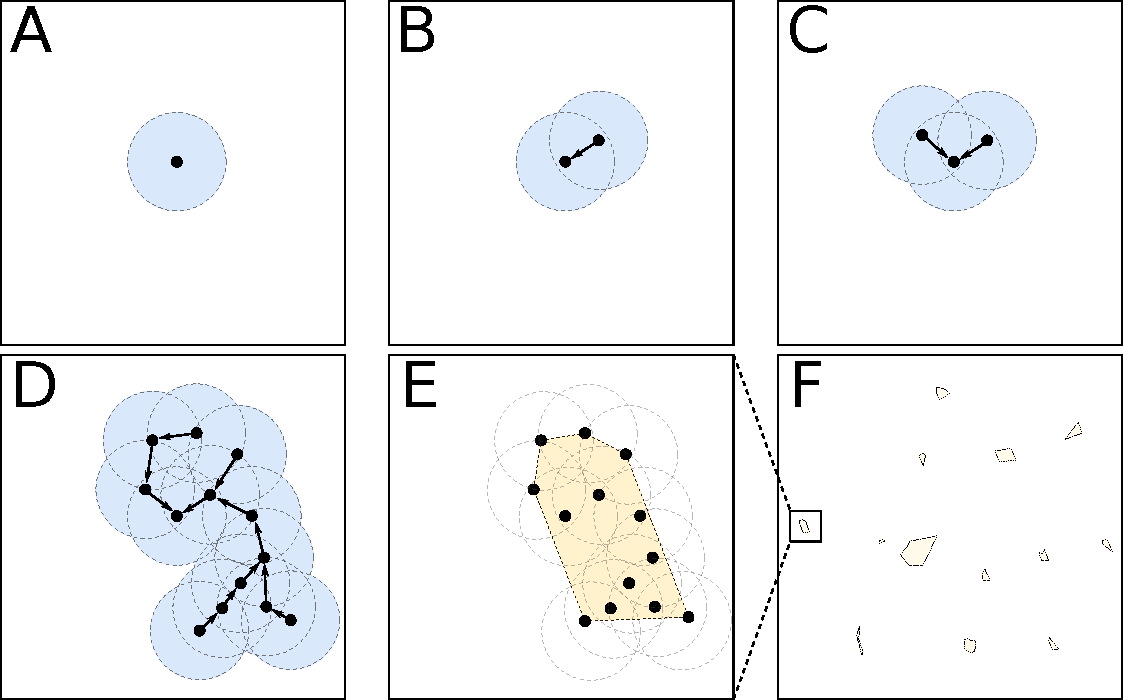
\includegraphics[width=.98\linewidth]{img/init_fp.pdf}
	\caption{Étapes successives de l'initialisation des foyers paysans agrégés (petites villes et villages).\\
	(A) On génère un foyer paysans ; (B) on génère un nouveau foyer paysan dans un rayon donnée du premier ; (C) et (D) on continue à générer de nouveaux foyers paysans dans le rayon de n'importe lequel des foyers existants ; (E) la géométrie d'un agrégat correspond à l'enveloppe convexe des foyers paysans ; (F) en fin d'initialisation, tous les agrégats initiaux sont répartis dans le monde.}
	\label{fig:init-fp}
\end{figure}



\subsection{Paramètres d'initialisation}

Dans la partie précédente, on a plusieurs fois indiqués que certaines des valeurs numériques de l'initialisation étaient paramétrables, c'est-à-dire qu'on peut les faire varier afin de générer des structures spatiales initiales différentes.
Cela participe à l'endogénéisation de l'espace support de SimFeodal, où il n'y a donc aucun \og \textit{input}\fg{}, mais un ensemble de paramètres régissant les différents sous-modèles.
Pour l'initialisation, les paramètres sur lesquels on peut jouer pour tester différents scénarios sont précisés dans le \cref{tab:params-initiaux}.


\begin{table}[H]
	\centering
		\caption{Paramètres permettant de contrôler l'initialisation du monde de SimFeodal.}
	\label{tab:params-initiaux}
	{\renewcommand{\arraystretch}{1.25}%
	\begin{tabular}{|M{2cm}|M{4cm}|m{5.25cm}|m{1.25cm}|}
		\hline
		\textbf{Sous-mécanisme} & \textbf{Paramètre} & \textbf{Intitulé} & \textbf{Valeur} \\ \hline
		\makecell{Création\\du monde} & Taille du monde & taille\_cote\_monde & 80 km \\ \hline
		\multirow{7}{*}{\makecell{Génération\\des\\Foyers\\Paysans}} & Nombre total de FP & init\_nb\_total\_fp & 4000 \\ \cline{2-4} 
		& Nombre de petites villes & init\_nb\_agglos & 8 \\ \cline{2-4} 
		& Nombre de FP par petite ville & init\_nb\_fp\_agglo & 30 \\ \cline{2-4} 
		& Nombre de villages & init\_nb\_villages & 20 \\ \cline{2-4} 
		& Nombre de FP par village & init\_nb\_fp\_village & 10 \\ \cline{2-4} 
		& Distance d'agrégation des FP & distance\_detection\_agregat & 100 m \\ \cline{2-4} 
		& Taux de FP \og dépendants\fg{} (ie. non mobiles) & proba\_fp\_dependant & 20\% \\ \hline
		\multirow{2}{*}{\makecell{Génération\\des\\Églises}} & Nombre total d'églises & init\_nb\_eglises & 150 \\ \cline{2-4} 
		& (dont) Nombre d'églises paroissiales & init\_nb\_eglises\_paroissiales & 50 \\ \hline
		\multirow{3}{*}{\makecell{Génération\\des\\Seigneurs}} & Nombre de Grands Seigneurs & init\_nb\_gs & 2 \\ \cline{2-4} 
		& \makecell{Puissance relatives\\des Grands Seigneurs} & \makecell{puissance\_grand\_seigneur$1$ \\ \textelp{} \\ puissance\_grand\_seigneur$N$} & 50\% \\ \cline{2-4} 
		& Nombre de Petits Seigneurs & init\_nb\_ps & 18 \\ \hline
	\end{tabular}}

\end{table}


\section[Données en entrée -- \textit{Input data}]{Données en entrée\protect\newline \large{\textit{Input data}} \sectionmark{Données en entrée}}

Comme indiqué, il n'y a pas véritablement d'\textit{inputs} dans SimFeodal : tout est paramètre, et donc dynamique.
En même temps, le modèle comporte de très nombreux paramètres : entre une quarantaine et une soixantaine selon les définitions possibles de ce qu'est un paramètre, voir \hl{chapitre 4}.\\
On peut donc voir dans la multiplicité des paramètres une proximité avec la notion de données en entrée, qui ne s'expriment toutefois pas sous la forme traditionnelle.

Par exemple, pour mettre en place des comportements exogènes permettant de faire varier le modèle à différentes dates précises, on peut classiquement faire appel à des données de sortie d'un autre modèle, ou à un fichier de configuration.
Dans SimFeodal, cette logique est bien présente, mais est gérée directement au sein du modèle, sans faire appel à des données externes : certains paramètres prennent ainsi la forme de tableaux d'associations (aussi appelés dictionnaires, ou \og \texttt{map}\fg{} en informatique), et font donc correspondre des valeurs de paramètres à des dates précises (voir \cref{lst:maps-gama}).
\medskip

{\footnotesize
\begin{lstlisting}[caption={
Deux exemples de \texttt{map} dans Gama.
\textit{À partir de 800, les églises doivent se situer entre 5 et 25~km, puis entre 3 et 10~km de 960 à 1060, et entre 1.5 et 5~km après cette date.}}, captionpos=b, label={lst:maps-gama}]
map<int,int> dist_min_eglise <- [800::5000,  960::3000,  1060::1500];
map<int,int> dist_max_eglise <- [800::25000, 960::10000, 1060::5000]; 
\end{lstlisting}
}

Pour respecter le formalisme ODD que suit ce chapitre, on peut au final considérer que SimFeodal est un modèle qui ne repose sur aucune donnée en entrée, quand bien même, conceptuellement, le rôle joué par les paramètres du modèle s'en approche fortement. Le \hl{chapitre 4} permet d'éclairer cette description en entrant plus en détail dans la définition et la nomenclature des paramètres.


\section[Mécanismes spécifiques -- \textit{Submodels}]{Mécanismes spécifiques\protect\newline \large{\textit{Submodels}} \sectionmark{Mécanismes spécifiques} \label{sec:meca-specifiques}}

\subsection{Introduction}

Cette partie du chapitre est plus technique, et vise à présenter précisément différents mécanismes de SimFeodal évoqués dans la partie relative au fonctionnement général du modèle (\cref{sec:fonctionnement-general}).
On ne vise ici pas l'exhaustivité, les détails d'implémentation étant bien trop nombreux pour être entièrement explicités, et parce que cela ferait un double-emploi assez conséquent en sus du code-source du modèle disponible à la consultation (voir l'\hyperlink{avant-propos}{avant-propos}).

Notons aussi que la présentation des mécanismes n'est pas nécessairement exacte, c'est-à-dire une description fidèle de la manière dont les mécanismes sont implémentés informatiquement sous forme de codes-sources.
Nous avons ici fait le choix de présenter les mécanismes sous la forme, discursive et schématique, la plus courte et compréhensible, quand bien même cette forme n'est qu'une \og équivalence\fg{} de la réalité de l'implémentation.
Ces écarts entre présentation discursive des mécanismes et implémentation effective sont discutés dans l'\cref{enc:polarite-implementation}.

On remarquera enfin que avons préféré présenter ces spécifiques dans un ordre différent de celui de l'ordonnancement dans le modèle (cf. \cref{fig:ordonnancement}), en les regroupant plutôt par les types d'agents concernés par chacun. On présentera d'abord les mécanismes \og globaux\fg{}, c'est-à-dire relevant de la détection des agrégats, pôles et des logiques de promotion et création de paroisses ; puis les mécanismes relatifs au foyers paysans et enfin ceux impliquant l'action des seigneurs.

\bigskip 
\begin{encadre}{Écarts entre présentation et implémentation}{polarite-implementation}
	
La présentation des mécanismes d'un modèle ne suit pas toujours la manière dont ces mécanismes sont implémentés dans le code-source d'un modèle.
C'est naturellement vrai entre deux \og domaines\fg{} d'un modèle (si l'on reprend la triade des domaines conceptuels, empirique et implémenté de \textcite{livet2014diversite}), au vu des écarts qu'il peut y avoir par exemple entre le modèle conceptuel et le modèle implémenté.
Toutefois, cela peut aussi se produire au sein d'un même domaine, par exemple ici pour le \og domaine du modèle\fg{}, c'est-à-dire dans l'implémentation du modèle.
La présentation discursive d'un modèle suit ses règles propres, par exemple la nécessité de suivre une progression linéaire, quand bien même faite d'allers-retours.
L'implémentation informatique, au contraire, ne suit pas forcément les mêmes règles, et tend même à requérir des logiques très différentes au nom d'une \og optimisation\fg{} du code-source, propre à chaque langage informatique.
Dans cet encadré, nous souhaitons mettre en avant trois types de processus où la présentation discursive et l'implémentation effective sont différentes tout en produisant des résultats équivalents.
Ces types de processus ne visent pas l'exhaustivité, mais sont des exemples rencontrés dans la présentation du modèle faite dans ce chapitre.

\paragraph{Perspective de l'implémentation} Quand un tirage aléatoire probabiliste est appliqué sur un grand nombre d'entités, son espérance théorique tend vers une fréquence empirique, en vertu de la loi des grands nombres.
En simulation à base d'agents, cela signifie que choisir une proportion de 10\% d'une large population (\og probabilité de groupe\fg{}) est quasi-équivalent à doter chacun des individus d'une probabilité de $0.1$ d'être choisis (\og probabilité individuelle\fg{}).
Cette équivalence est fortement mobilisée dans SimFeodal, la perspective\fg{} -- probabilité individuelle ou de groupe -- changeant parfois à plusieurs reprises dans un même mécanisme, selon la praticité ou la performance (informatique) de l'une ou l'autre.
Dans la description du modèle, où on essaie d'avoir la vision la plus \og agent-centrée\fg{} possible, on présentera donc préférentiellement des mécanismes comme faisant appel à des probabilités individuelles, quand bien même l'implémentation effective se baserait sur une approche proportionnelle, mobilisant des probabilités de groupe.

\paragraph{Factorisation} Une autre différence tient à l'ordre d'exécution des sous-mécanismes par un ensemble d'agents. En mathématiques, $k\times (x+y)$ est égal, selon les règles de factorisation, à $k{\cdot}x + k{\cdot}y$.
Dans un système multi-agent, la logique est la même, quand bien même l'ordre d'appel des agents peut faire varier le résultat et l'on considère donc à nouveau qu'il s'agit d'une équivalence plus que d'une égalité : les programmes \ref{lst:facto1} et \ref{lst:facto2} sont équivalents.\bigskip

\noindent\begin{minipage}[b]{.45\textwidth}
	\begin{lstlisting}[caption={Factorisé},frame=tlrb, captionpos=b, label = {lst:facto1}]
ask agents [
  do A;
  do B;
]
	\end{lstlisting}
\end{minipage}\hfill
\begin{minipage}[b]{.45\textwidth}
	\begin{lstlisting}[caption={Développé},frame=tlrb, captionpos=b, label = {lst:facto2}]
ask agents [
  do A; ]
ask agents [
  do B; ]
	\end{lstlisting}
\end{minipage}

En terme d'efficacité du code, à nouveau, l'alternance entre ces approches d'implémentation permet de résoudre certaines difficultés d'implémentation plus simplement, par exemple en permettant la factorisation de calculs légers et au contraire le développement, pour stockage intermédiaires entre autre, de calculs plus lourds.
Pour bien différencier les étapes successives, dans le cadre d'une description discursive, il sera souvent plus aisé de présenter les sous-processus de manière développée plutôt que factorisée, ce qui, encore une fois, n'implique rien quant à l'implémentation réelle.

\paragraph{Optimisation} Les deux types de processus précédents peuvent être combinés, pour répondre à des questions d'optimisation informatique, c'est-à-dire par exemple permettre au modèle de fonctionner plus rapidement en fonction des spécificités des langages informatiques choisis.
Dans Gama, par exemple, il est plus lent, informatiquement, de calculer la distance depuis 1000 agents à 10 agents, que l'inverse, quand bien même les résultats sont ici strictement identiques.
Pour le calcul de la satisfaction de protection des foyers paysans par exemple, qui demande à chacun de mesurer sa distance au château le plus proche, il est bien plus rapide de calculer, depuis la perspective des châteaux, la distance aux différents foyers paysans en en prenant le minimum.
Dans cet exemple, l'implémentation se fait donc dans un sens opposé à celui du discours, sans que cela n'ait la moindre conséquence -- au niveau du domaine conceptuel, empirique, ou même en termes de mécanisme implémentés --, sinon une plus grande optimisation du fonctionnement informatique du modèle.
\end{encadre}

\subsection{Mécanismes globaux}

\subsubsection{Identification des agrégats \label{sssec:agregats}}
	
\begin{figure}[H]
	\centering
	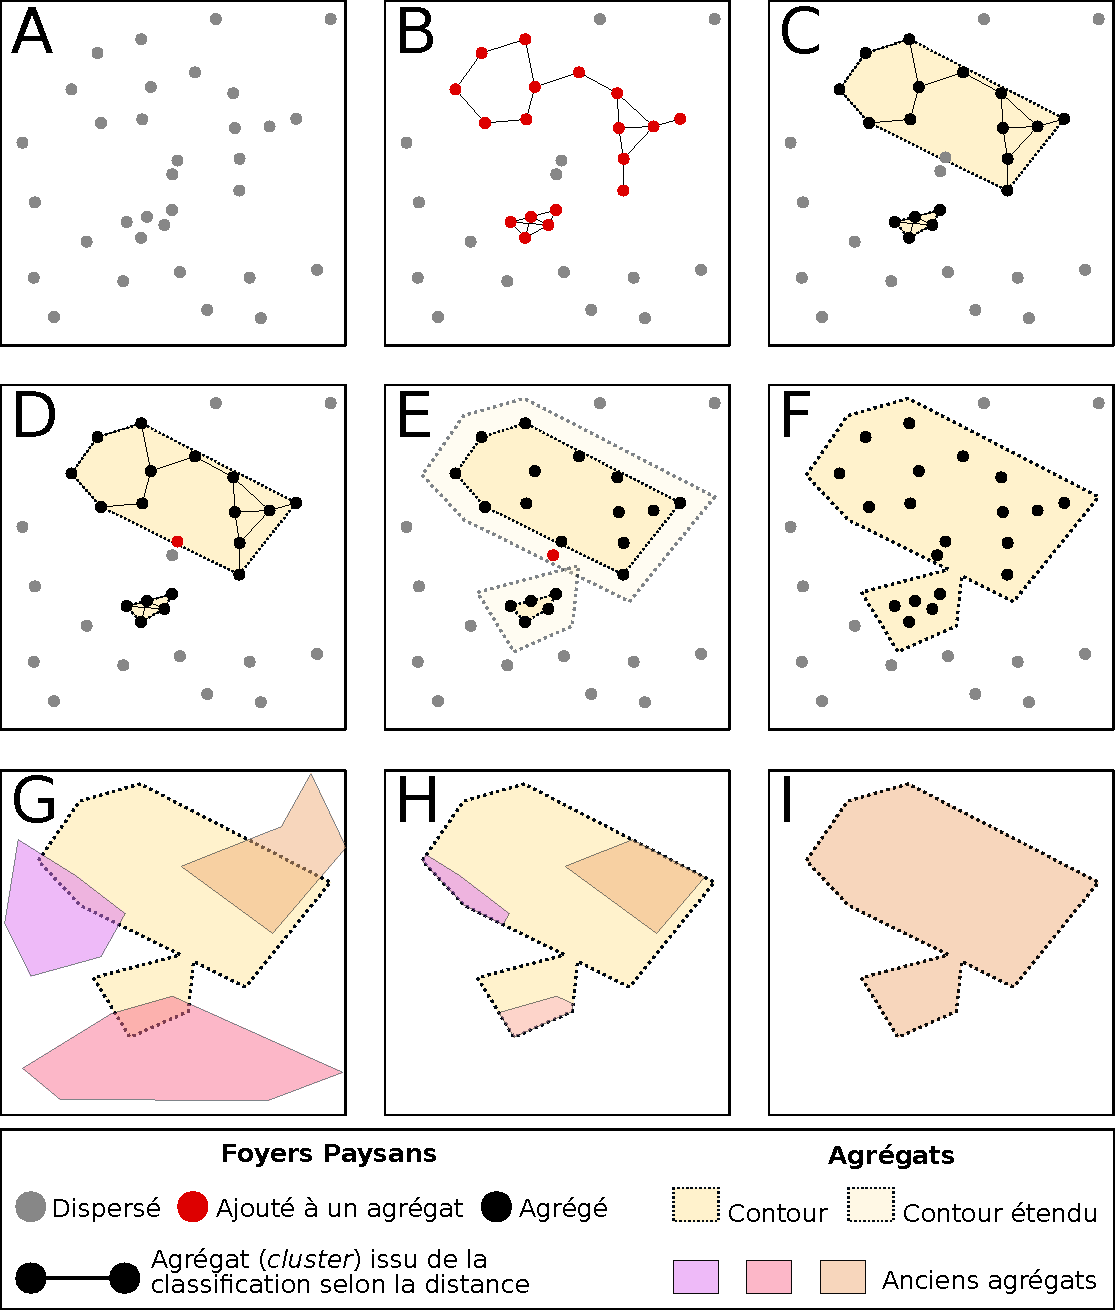
\includegraphics[width=.75\linewidth]{img/detection_agregats.pdf}
	\caption{Détection et de l'héritage des agrégats.}
	\label{fig:detection-agregats}
\end{figure}

La \cref{fig:detection-agregats} présente les étapes successives de détection des agrégats.
À chaque pas de temps, on repart d'une situation \og neutre\fg{}, c'est-à-dire que tous les foyers paysans sont considérés comme dispersés (\textbf{A}).
On exécute un algorithme de classification basé sur la distance, proche de DBSCAN : les \textit{clusters} constitués d'au moins 5 foyers paysans espacés de moins de 100~m sont considérés comme des agrégats(\textbf{B}).
On fixe alors la géométrie des agrégats, qui prend la forme de l'enveloppe convexe des foyers paysans qui les composent (\textbf{C}).
Les foyers paysans inclus dans la surface d'un agrégat y sont ajoutés (\textbf{D}).
On crée ensuite des \textit{buffers} de 100~m autour des agrégats et on y rattache à nouveau les foyers paysans inclus dans la surface (\textbf{E}).
Dernière étape dans la détection des agrégats, et afin de ne pas multiplier les agrégats proches les uns des autres, on procède à une étape de fusion : on réalise l'union géométrique des agrégats qui s'intersectent (\textbf{F}).\\
Les trois dernières étapes concernent la transmission des propriétés des agrégats à travers les pas de temps, et en particulier de la présence ou non d'une communauté en leur sein.
On isole les agrégats du pas de temps précédent qui intersectent les nouveaux agrégats (\textbf{G}).
On procède ensuite à une intersection entre les géométries de ces anciens agrégats et le nouvel agrégat (\textbf{H}).
Le nouvel agrégat hérite alors des propriétés de l'ancien agrégat dont la superficie d'intersection est la plus importante, c'est-à-dire l'agrégat orange ici (\textbf{I}).
	
	\subsubsection{Identification des pôles \label{sssec:poles}}

\begin{figure}[H]
	\centering
	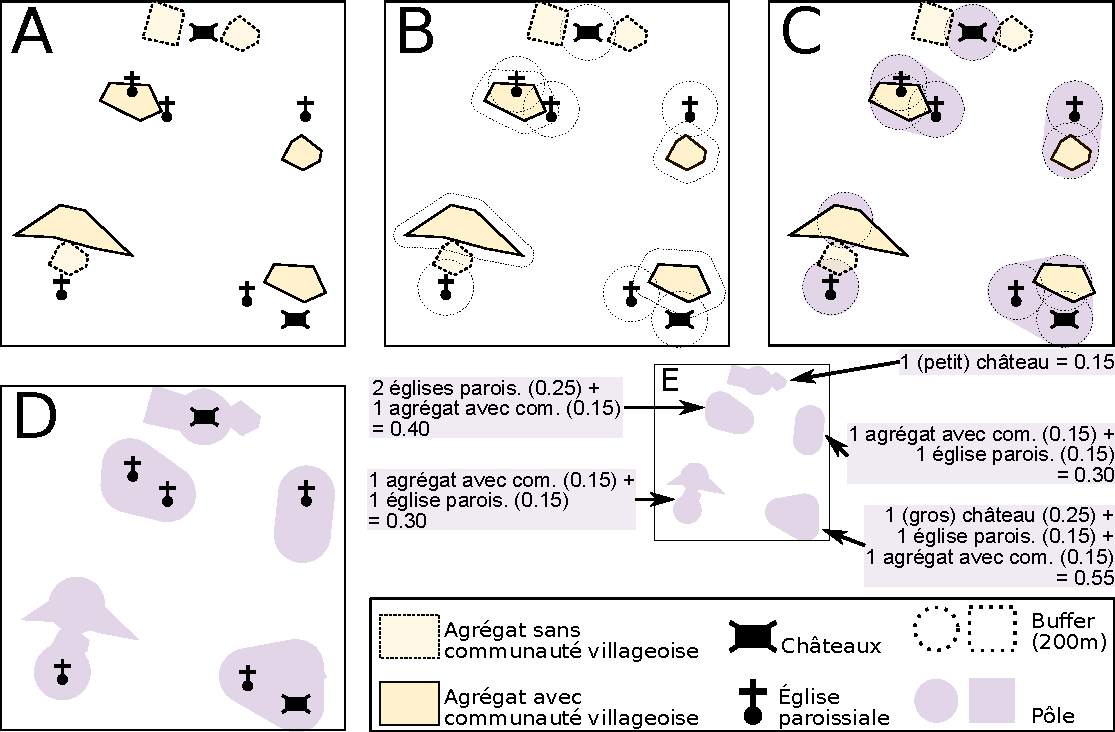
\includegraphics[width=\linewidth]{img/detection_poles.pdf}
	\caption{Les étapes du mécanisme de détection et de calcul d'attractivité des pôles.}
	\label{fig:detection-poles}
\end{figure}

Les pôles sont des agents composés d'attracteurs de trois types : les châteaux (petits et gros), les églises (uniquement celles dotées de droits paroissiaux) et les agrégats (uniquement ceux comportant une communauté paysanne).
Les pôles et leur délimitation spatiale revêtent une importance particulière lors de la migration des foyers paysans : ils attirent d'autant plus que leur attractivité est importante, et le cas échéant, les foyers paysans migrants s'installent à l'intérieur de leur délimitation.
La \cref{fig:detection-poles} illustre la méthode de définition spatiale des pôles, ainsi que des exemples de calcul de leurs attractivités.

À chaque pas de temps, on repart d'une situation \og neutre\fg{}, c'est-à-dire que l'on recalcule systématiquement les pôles sans repartir des pas de temps précédents (\textbf{A}).
On commence par identifier les attracteurs situés à moins de 200~m les uns des autres (\textbf{B}) pour identifier les pôles : ceux-ci peuvent être constitués de plusieurs attracteurs proches, ou d'un unique attracteur.
L'enveloppe spatiale des pôles est définie comme un \textit{buffer} de 200~m autour de l'enveloppe convexe formée par le centroïde des attracteurs qui les composent (\textbf{C}). Il s'agit donc d'un cercle de rayon de 200~m pour les pôles mono-attracteurs, et d'un polygone pour les pôles composites.
Afin de renforcer la probabilité de voir croître les agrégats à proximité des pôles, on fusionne (union géométrique) l'enveloppe spatiale des pôles avec les contours de l'ensemble des agrégats (comportant ou non une communauté paysanne) intersectés, ce qui peut permettre à des pôles peu éloignés de fusionner à leur tour (\textbf{D}).
On peut alors calculer leur attractivité en se reportant au \cref{tab:attraction-poles} (p.~\pageref{tab:attraction-poles}) (\textbf{E}).


	
	\subsubsection{Création et promotion d'églises paroissiales \label{sssec:paroisses}}
	
	\begin{figure}[H]
		\centering
		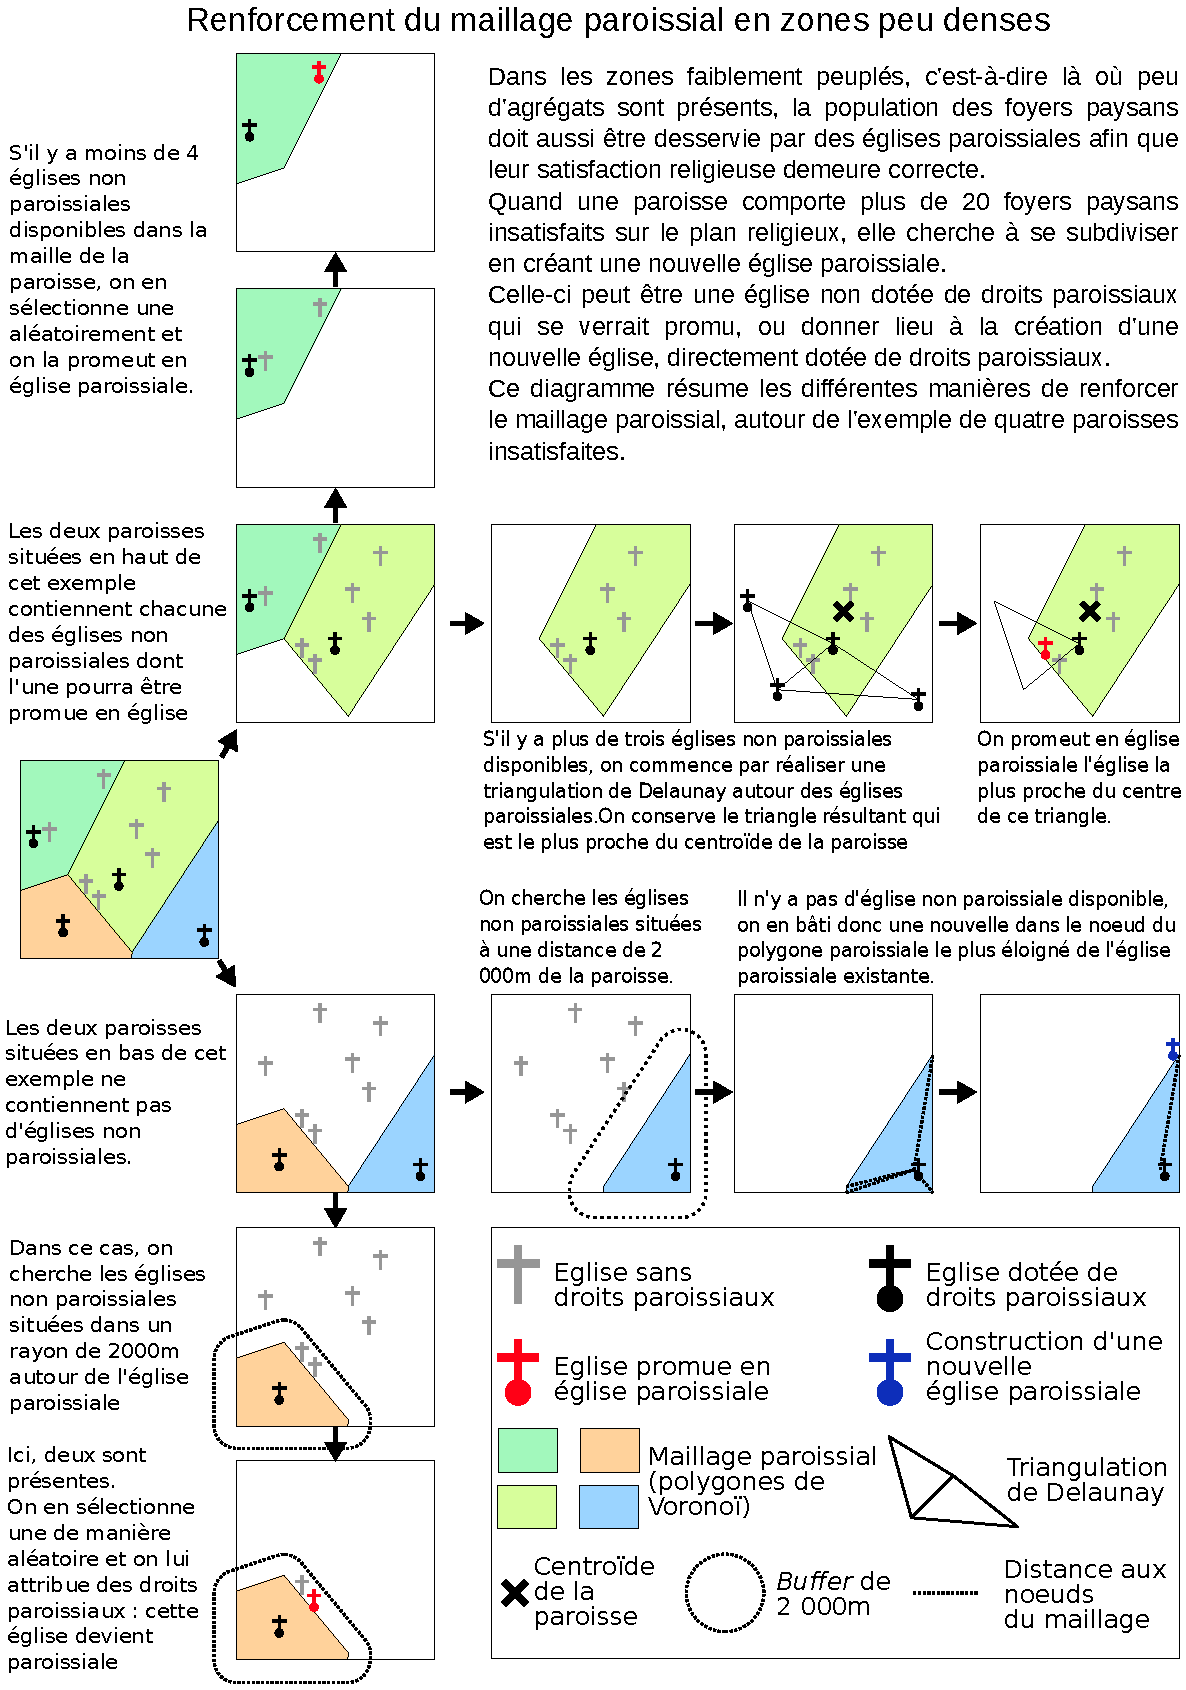
\includegraphics[width=1\linewidth]{img/constru-promo_paroisses_rurales.pdf}
		\caption{Construction et promotion de paroisses en zone peu dense.}
		\label{fig:promotion-paroisses}
	\end{figure}
	
\clearpage
\subsection{Foyers paysans}

	\subsubsection{Satisfaction et modèles gravitaires \label{sssec:satisfaction}}
	
Les sastisfactions religieuses et de protection des foyers paysans suivent une logique proche du modèle gravitaire : plus les foyers sont éloignés des \og attracteurs\fg{} (les châteaux pour la satisfaction protection ; les églises paroissiales pour la satisfaction religieuse), moins ils sont satisfaits.
Cette logique simple est légèrement contrainte en ajoutant des seuils : en dessous d'une certaine distance (\textit{distance\_min}), le foyer paysan est entièrement satisfait (satisfaction = 1), et au delà d'une autre distance (\textit{distance\_max}), sa satisfaction est nulle (satisfaction = 0).
Entre ces deux seuils, minimaux et maximaux, la satisfaction suit une logique gravitaire simple, soit ici une décroissance linéaire.
L'équation \ref{eq:satisfaction-distance} permet de formaliser ce type de calcul, et la \cref{fig:satisfaction-distance} l'illustre de manière sans doute plus accessible.

\begin{figure}[H]
	\centering
	\begin{equation}\label{eq:satisfaction-distance}
	\begin{gathered}
	satis\_dist = min  \left \lbrack max \left \lbrack \frac{(distance\_max - distance\_attracteur)}{(distance\_max -distance\_min)}; 0 \right \rbrack ; 1 \right \rbrack
	\end{gathered}
	\end{equation}
	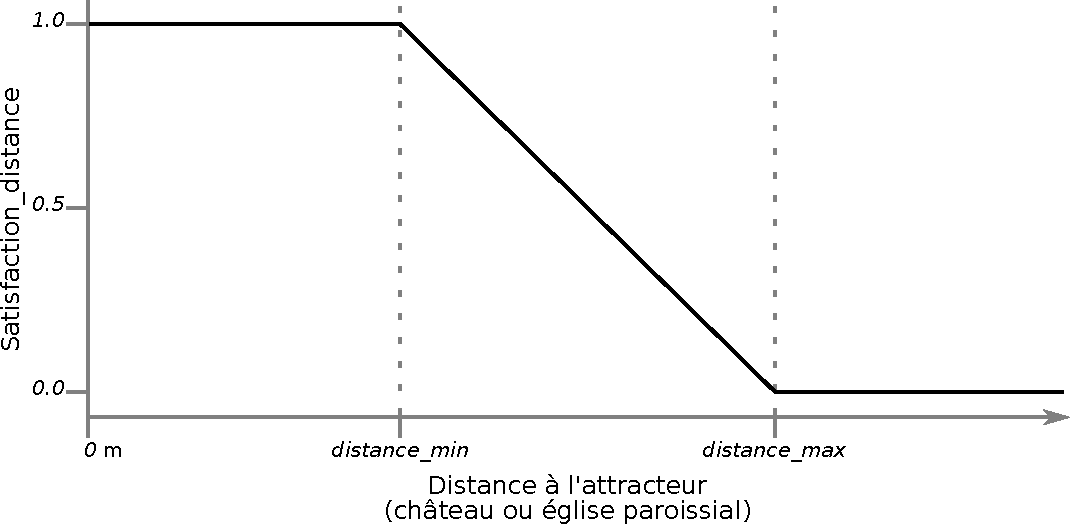
\includegraphics[width=.8\linewidth]{img/satisfaction_distance.pdf}
	\caption{Évolution de la satisfaction en fonction de la distance à l'attracteur le plus proche.}
	\label{fig:satisfaction-distance}
\end{figure}

\paragraph{Satisfaction religieuse}
		
Le calcul de la satisfaction religieuse s'inscrit rigoureusement dans cette logique, et sa formule, dépendant de paramètres qui évoluent en fonction du temps, est donc :
		\begin{equation*}
		s_{religieuse} = min  \left \lbrack max \left \lbrack \frac{(distance_{max} - distance\_eglise)}{(distance_{max} -distance_{min})}; 0 \right \rbrack ; 1 \right \rbrack
		\end{equation*}
avec les seuils de distance ($distance\_max$ et $distance\_min$) qui évoluent au cours du temps de telle manière :
\begin{itemize}
	\item avant 960 : $distance_{min}$ = 5 km et $distance_{max}$ =  25 km
	\item de 960 à 1060 : $distance_{min}$ = 3 km et $distance_{max}$ =  10 km
	\item après 1060 : $distance_{min}$ = 1,5 km et $distance_{max}$ =  5 km
\end{itemize}
	
\paragraph{Satisfaction protection}	

La satisfaction protection mobilise une logique proche, c'est-à-dire qu'elle est fonction de la distance au château le plus proche, pondérée toutefois par un paramètre ($besoin\_protection$) qui permet de pondérer la réaction face à un climat de violence qui tend à augmenter pendant la période.

\begin{equation*}
s_{protection} = (s_{distance\_chateau})^{(besoin\_protection)}
\end{equation*}
avec
\begin{equation*}
\begin{gathered}
s_{distance\_chateau} = min  \left \lbrack
max \left \lbrack \frac{(dist_{max} - distance\_chateau)}{(dist_{max} -distance_{min})}; 0.01 \right \rbrack ; 1 \right \rbrack
\end{gathered}
\end{equation*}
($dist_{min}$ = 1,5 km et $dist_{max}$ = 5 km )
et le besoin de protection évolutif :
\begin{itemize}
	\item avant 960 : $besoin\_protection = 0 $
	\item de 960 à 1020 : $besoin\_protection = 0.2 ; 0.4 ; 0.6 ; 0.8$
	\item après 1020 : $besoin\_protection = 1$
\end{itemize}

\paragraph{Satisfaction matérielle}

La satisfaction matérielle ne prend aucune distance en compte : elle s'appuie sur le montant des taxes dont le foyer paysan doit s'acquitter ($redevance\_acquittees$), pondérée par un paramètre technique représentant un niveau \og acceptable\fg{} de taxation ($coef\_redevances$, qui vaut $15$ ici).
L'appartenance du foyer paysan à une communauté fini de contre-balancer le montant des redevances acquittées, sous la forme d'un contre-poids dont l'importance augmente au fur et à mesure de la période modélisée ($puissance\_communaute$ vaut $0.2$ jusqu'en 1060, puis augmente de $0.2$ à chaque pas de temps pour atteindre $1$ en 1040 et rester à ce niveau).

\begin{equation*}
\begin{gathered}
s_{materielle} = (s_{redevance})^{(1-puissance\_communaute)}
\end{gathered}
\end{equation*}
avec 
\begin{equation*}
\begin{gathered}
s_{redevance} = max \left[ \left( 1- \frac{redevances\_acquittees}{coef\_redevances} \right) ; 0 \right]
\end{gathered}
\end{equation*}

\paragraph{Satisfaction générale}

La satisfaction générale est mesurée en prenant le minimum de ces satisfaction individuelles, c'est-à-dire qu'on considère qu'elles ne s'équilibrent pas.
Comme pour la satisfaction matérielle qui la compose, l'appartenance du foyer paysan à une communauté paysanne tend aussi à augmenter la satisfaction générale : cela intervient donc à deux reprises dans le calcul de la satisfaction, afin d'illustrer le poids que prennent ces structures sociales et institutionnelles au cours de la période modélisée.

Le calcul de la satisfaction s'exprime donc ainsi :
\begin{equation*}
\begin{gathered}
\begin{split}
satisfaction =~& 0.75 \times \left[ min \left( s_{materielle} ; s_ {religieuse}; s_{protection} \right) \right] + \\
& 0.25 \times [appartenance\_communaute]
\end{split}
\end{gathered}
\end{equation*}
avec $ \{satisfaction ; s_{materielle} ; s_ {religieuse} ; s_{protection}\} \in [0,1]$ et $[appartenance\_communaute] \in \{0;1\} $


	\subsubsection{Migration des foyers paysans \label{sssec:migration}}

La migration des foyers paysans est sans doute le mécanisme le plus complexe et ayant subi les plus fortes évolutions depuis la conception de SimFeodal.
La règle d'ensemble est pourtant extrêmement simple : un foyer paysan a une probabilité de migrer qui est inversement proportionnelle à sa satisfaction. Autrement dit, $P \left( migration \right) = \left( 1 - satisfaction \right)$.
Cette règle simple a été progressivement complexifiée afin d'augmenter la rationalité et l'ancrage empirique des choix de localisation : une première complexification a abouti à la distinction de migrations \og locales\fg{} et de migrations \og lointaines\fg{} (voir \cref{fig:migrations-locales-lointaines}).

\begin{figure}[H]
\centering
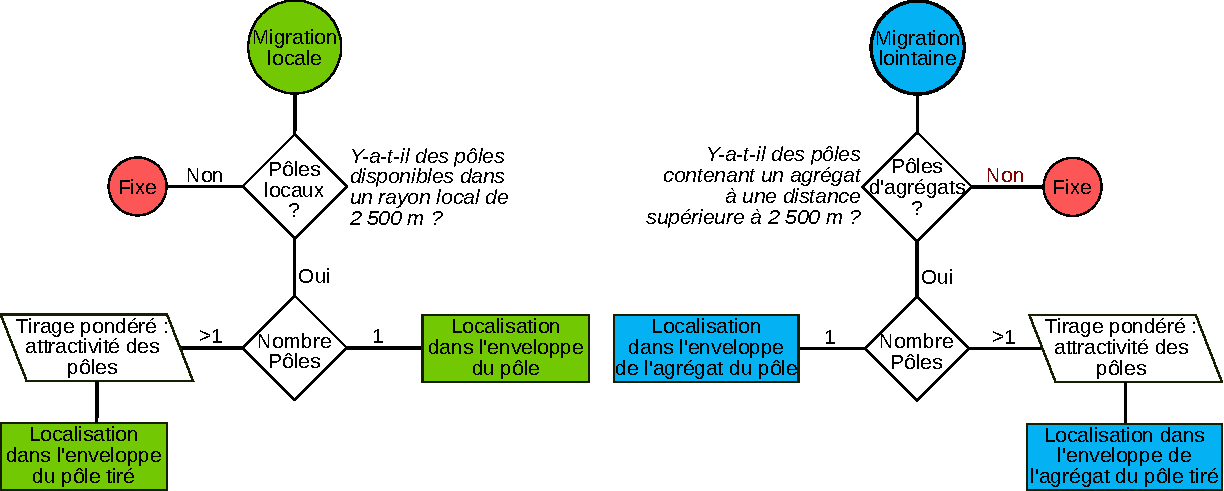
\includegraphics[width=1\linewidth]{img/migration_locale-lointaine.pdf}
\caption{Migrations locales et lointaines.}
\label{fig:migrations-locales-lointaines}
\end{figure}
Pour aboutir à cette différence entre migration locale et migration lointaine, la règle est encore une fois complexe : les foyers paysans privilégient les migrations locales, et quand celles-ci ne sont pas possibles, ils ont une probabilité plus faible d'effectuer une migration lointaine. Notons que pour nous approcher des connaissances empiriques, nous avons établi un comportement légèrement différent entre les foyers paysans déjà agrégés et ceux qui seraient dispersés lors de l'exécution du mécanisme de migration (\cref{fig:choix-migration}).
\begin{figure}[H]
	\centering
	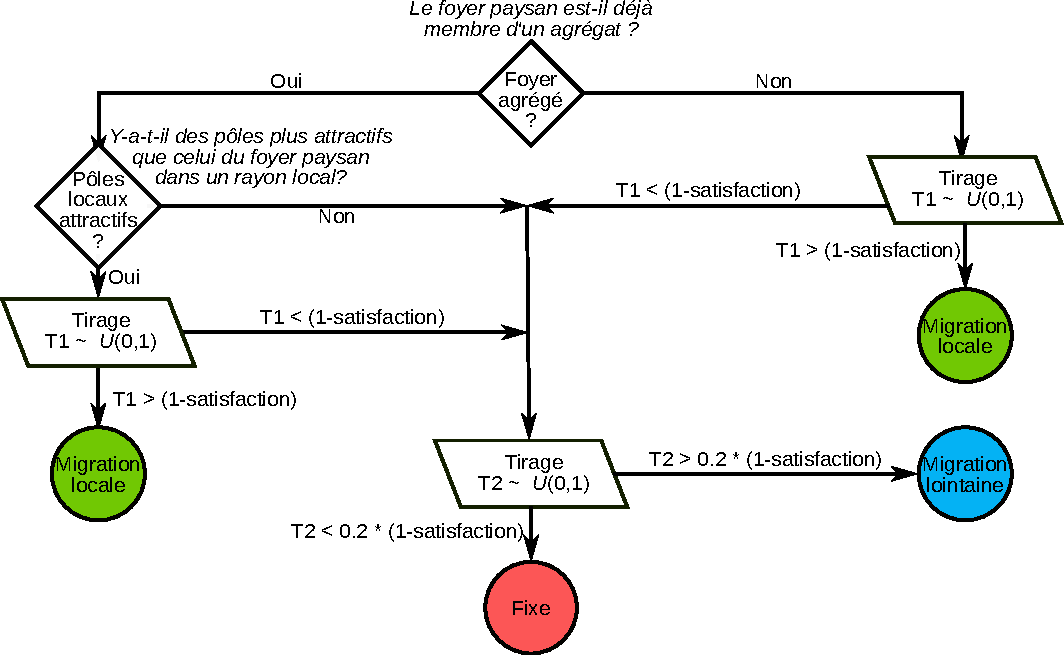
\includegraphics[width=0.9\linewidth]{img/choix_migration.pdf}
	\caption{Décision de migration.}
	\label{fig:choix-migration}
\end{figure}

Une dernière distinction a été opérée entre les foyers paysans classiques, libres de leurs migrations, et les foyers paysans \og dépendants\fg{}, qui représentent ceux qui n'avaient pas le droit de quitter le domaine de leur seigneur (les serfs entre autres). Ceux-là ne peuvent effectuer que des migrations locales, et on considère qu'ils seront amenés à migrer plus facilement, ce qui change encore une fois leur mécanisme de migration (\cref{fig:choix-migration-dependants}).
\begin{figure}[H]
	\centering
	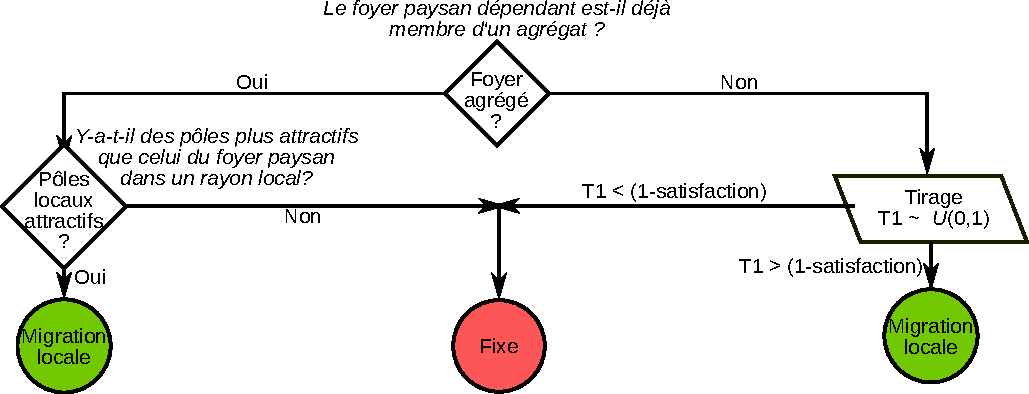
\includegraphics[width=0.9\linewidth]{img/choix_migration_dependants.pdf}
	\caption{Décision de migration des foyers paysans dépendants.}
	\label{fig:choix-migration-dependants}
\end{figure}
 

	
\subsection{Seigneurs}
	\subsubsection{Prélèvement des droits \label{sssec:collecte-droits}}

Les seigneurs, petits et grands, collectent les droits dont doivent s'acquitter les foyers paysans (droits de haute justice et autres droits) majoritairement (exception faite des droits fonciers pour les grands seigneurs, voir \cref{fig:prelevement-fonciers}) par l'intermédiaire des zones de prélèvement.
Ces zones sont caractérisées par un propriétaire (le seigneur qui les possèdent), éventuellement un gardien (le seigneur à qui la zone a été \og donnée\fg{}, voir \cref{meca-dons}), une localisation (pour les petits seigneurs, il s'agit de leur propre localisation), un rayon\footnote{
Ce rayon est tiré aléatoirement suivant une distribution uniforme, \\$rayon\_zp \sim \mathcal{U}\left[ rayon\_min\_zp\_ps , rayon\_max\_zp\_ps \right]$, avec $rayon\_min\_zp\_ps$ et $rayon\_max\_zp\_ps$ des paramètres qui valent respectivement 1 000 et 5 000 m.
} et un taux de prélèvement\footnote{
idem : $taux\_prelevement\_zp \sim \mathcal{U}\left[ min\_taux\_prelevement\_zp\_ps , max\_taux\_prelevement\_zp\_ps \right]$ avec $min\_taux\_prelevement\_zp\_ps$ et $max\_taux\_prelevement\_zp\_ps$ valant 5\% et 25\%.
}.
A noter que les zones de prélèvement liées à des châteaux suivent une règle légèrement différente, que nous n'aborderons pas ici\footnote{Se référer au code-source du modèle, dans la fonction \textsf{construction\_chateaux}}.

Les prélèvements, selon les types de droits, rapportent de la \og puissance\fg{} aux seigneurs, dont le \cref{tab:puissance-droits} donne une référence.

\begin{table}[H]
	\centering
	\caption{Gain de puissance par foyer paysan prélevé.}
	\label{tab:puissance-droits}
	{\renewcommand{\arraystretch}{1.1}%
		\begin{tabular}{|l|l|l|}\hline
			\textbf{Type de droit} & \textbf{Fonction du seigneur} & \textbf{\makecell{Puissance acquise\\par foyer paysan}} \\ \hline
			\multirow{2}{*}{Haute Justice} & Propriétaire ou Gardien & 2 \\
			& Souverain (zone donnée) & 2.5 \\ \hline
			\multirow{2}{*}{Droits fonciers} & Propriétaire ou Gardien & 1 \\
			& Souverain (zone donnée) & 1.25 \\ \hline
			\multirow{2}{*}{Autres droits} & Propriétaire ou Gardien & 0.25 \\
			& Souverain (zone donnée) & 0.35 \\ \hline	
	\end{tabular}}
\end{table}


\paragraph{Foncier}

Quelques petits seigneurs (ceux créés dès l'initialisation ainsi que $\approx 10\%$ de ceux créés pendant le déroulement de la simulation) possèdent des droits fonciers, et à ce titre, peuvent collecter ces droits au sein d'une zone de prélèvement qu'ils créent lors de leur apparition. Le mécanisme de collecte des droits fonciers est illustré dans la \cref{fig:prelevement-fonciers}.
\begin{figure}[H]
	\centering
	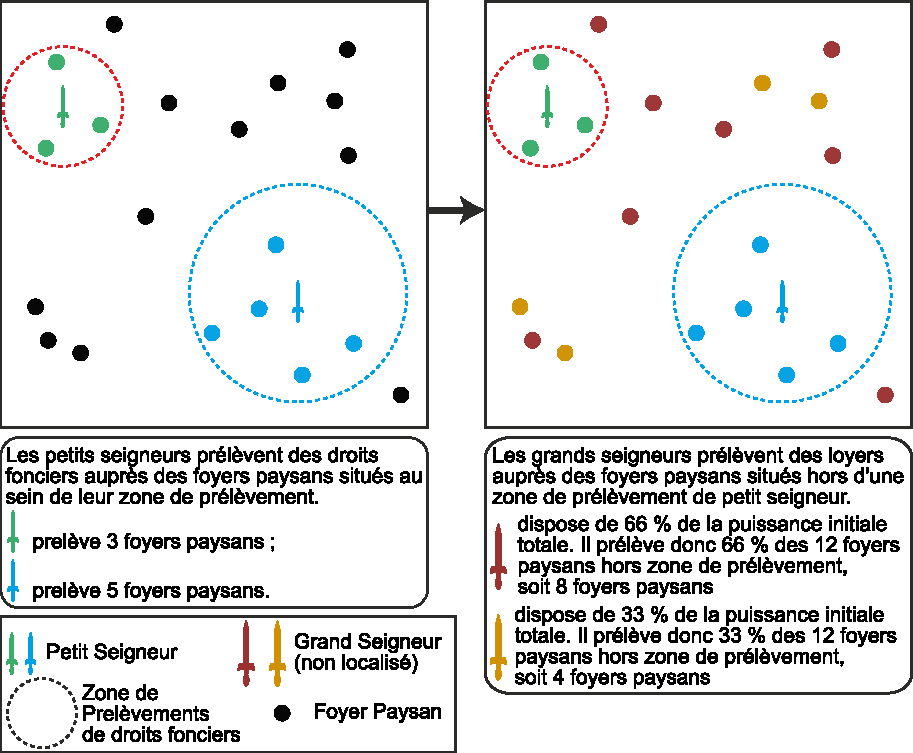
\includegraphics[width=0.8\linewidth]{img/prelevements_foncier.pdf}
	\caption{Prélèvement des droits fonciers par les petits et grands seigneurs.}
	\label{fig:prelevement-fonciers}
\end{figure}

\paragraph{Haute justice et autres droits}

Les autres droits suivent un mécanisme plus générique : les seigneurs propriétaires collectent des droits auprès d'une partie des foyers paysans inclus dans la surface de la zone de prélèvement. Cette partie correspond aux \og taux de prélèvement\fg{} décrit plus haut. La \cref{fig:prelevement-droits} récapitule les différentes modalités de collecte de droits via les zones de prélèvement.

\begin{figure}[H]
	\centering
	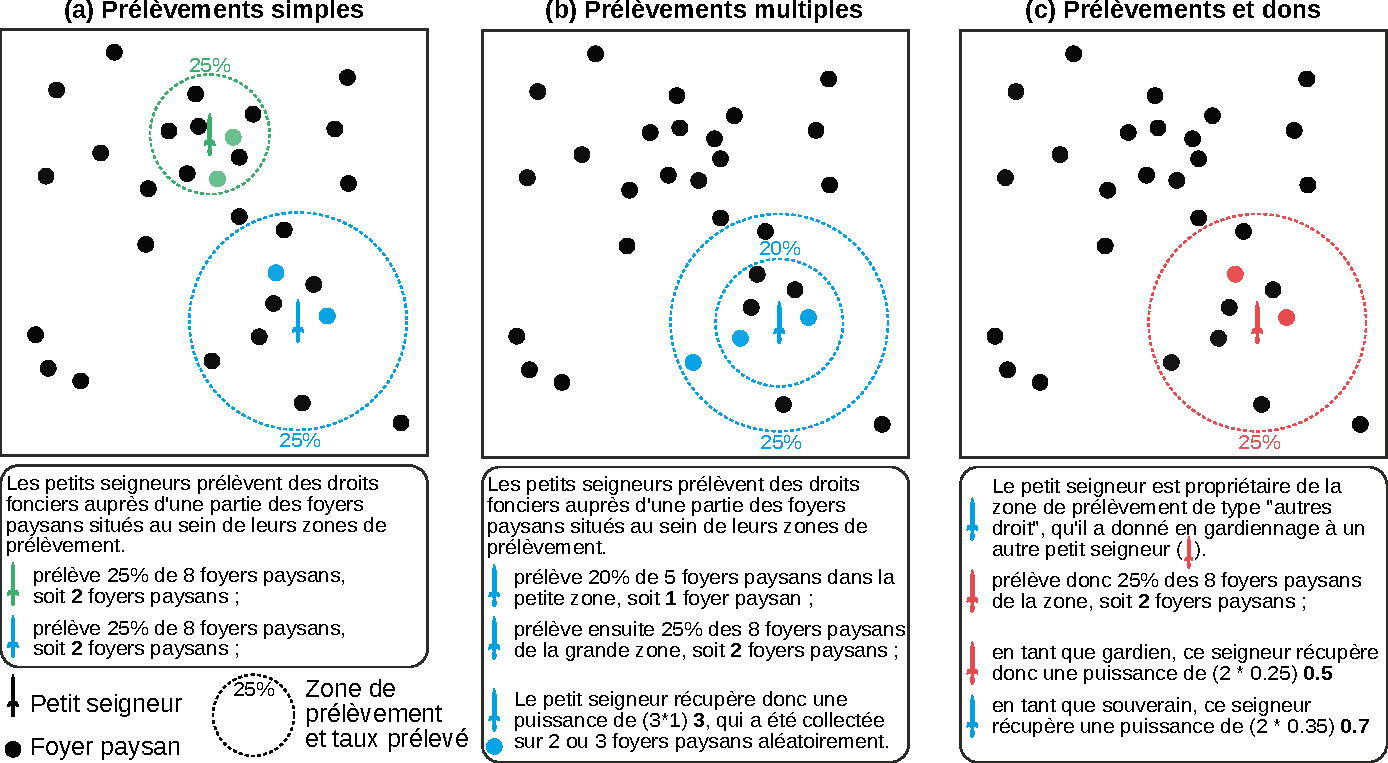
\includegraphics[width=\linewidth]{img/prelevements_droits.pdf}
	\caption{Mécanisme général de prélèvement des droits par les seigneurs.}
	\label{fig:prelevement-droits}
\end{figure}

Les droits de haute justice sont prélevés exactement comme les autres droits, à la seule différence qu'ils correspondent nécessairement à des taux de prélèvement de 100\%.

\subsubsection{Construction de châteaux \label{sssec:constru-chateaux}}


À partir de 940, les seigneurs ont la possibilité de créer des châteaux.
Le mécanisme de construction des châteaux est commun aux grands et aux petits seigneurs, mais certains paramètres varient selon le type du seigneur considéré :
\begin{itemize}
	\item Un grand seigneur peut constuire jusqu'à $2$ châteaux par tour (paramètre $nb\_max\_chateaux\_par\_tour\_gs$), alors qu'un petit seigneur ne peut en construire au maximum que $1$ par pas de temps ($nb\_max\_chateaux\_par\_tour\_ps$).
	\item Pour un seigneur $i$, la probabilité de construire un château est formalisée ainsi :\\
	$$ P \left( construction \right) =  \frac{puissance\_seigneur_{i}}{\sum{puissance\_seigneur}} \times ponderation\_proba\_chateau $$ avec $ponderation\_proba\_chateau$ valant $1.25$ pour les grands seigneurs et $7$ pour les petits (paramètres techniques).
	\item Les grands seigneurs peuvent construire des châteaux n'importe-où dans l'espace du modèle (en respectant toutefois les règles exposées plus bas), alors que les petits seigneurs ne peuvent le faire que dans un rayon de 5 000 m de leur localisation : s'il n'y a pas d'espace disponible dans ce rayon, le petit seigneur ne crée pas de château.
\end{itemize}

Les règles de localisation de château sont identiques, et illustrés dans la \cref{fig:construction-chateaux}.

\begin{figure}[H]
	\centering
	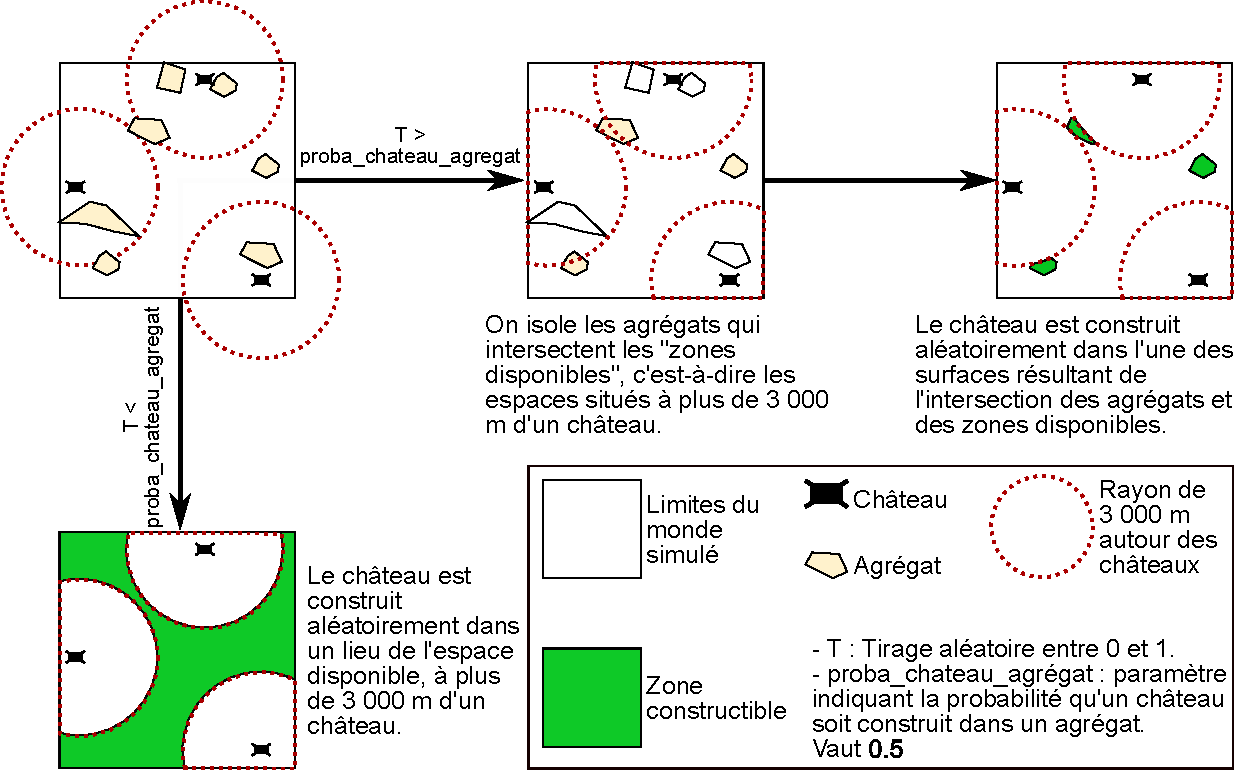
\includegraphics[width=\linewidth]{img/construction_chateaux.pdf}
	\caption{Mécanisme de localisation des châteaux construits.}
	\label{fig:construction-chateaux}
\end{figure}

\paragraph{Rayon des zones de prélèvement associées}

La construction d'un château implique systématiquement la création de zones de prélèvements qui lui sont associées, c'est-à-dire qu'elles appartiennent au seigneur qui crée le château.
Si le château est donné en gardiennage, l'ensemble des zones de prélèvement qui lui sont associées seront aussi données en gardiennage au petit seigneur choisi.

Les zones de prélèvement créées concernent des droits fonciers et des autres droits.
Si le seigneur châtelain obtient les droits de haute justice, une zone de prélèvement de droits de haute justice sera automatiquement créée autour de chacun de ses châteaux.
Contrairement aux zones de prélèvement habituelles, celles qui sont associées à un château ont un taux de prélèvement de $100\%$.
Leur rayon est variable et dépend de la puissance relative du seigneur qui construit le château.
Ce rayon varie entre un seuil minimal de 2 000 m ($rayon\_min\_zp\_chateau$) et un seuil maximal de 15 000 m ($rayon\_max\_zp\_chateau$).
Entre ces deux seuils, la valeur du rayon dépend d'une fonction linéaire correspondant au ratio entre la puissance du seigneur constructeur et les puissances maximales et minimales de l'ensemble des seigneurs, tel que formalisé dans l'équation \ref{eq:rayon-zp-chateau}. 

\begin{equation}\label{eq:rayon-zp-chateau}
\begin{aligned}
& rayon\_zp\_chateau = \\
& min  \left[ max \left[ puissance\_relative; rayon\_min\_zp\_chateau \right]  ; rayon\_max\_zp\_chateau \right]
\\
& \text{avec}
\\
& puissance\_relative_i = \frac{max(puissance_{0..n}) - puissance_i}{max(puissance_{0..n}) \times min(puissance_{0..n})}
\end{aligned}
\end{equation}

\section*{Conclusion}
\addcontentsline{toc}{section}{Conclusion}

\printbibliography[title={Références}]


%\graphicspath{{chap3/}}
%\setcounter{chapter}{2}
%% !TeX root = chap3.tex
% !TeX encoding = UTF-8
% !TeX spellcheck = fr_FR
\documentclass[12pt, a4paper, oneside]{book}
%\usepackage[utf8]{inputenc}
\usepackage{amsmath}
\usepackage{amsfonts}
\usepackage{amssymb}
\usepackage{graphicx}
\usepackage[left=1.5cm, right=5cm, bottom = 1cm, top = 2cm, headheight=16pt,
headsep = 0.5cm, foot = 16pt, footskip = 0.5cm]{geometry}
\setlength{\marginparwidth}{4.5cm}
\usepackage{marginnote}

\usepackage{fontspec}
\setmainfont{Charis SIL}
\usepackage{setspace}
\setstretch{1.1}
\usepackage[french]{babel}
\usepackage[babel=true]{csquotes}

\usepackage{soul}
\usepackage{mdframed}

\usepackage{xargs} % Use more than one optional parameter in a new commands
\usepackage[dvipsnames]{xcolor}


\usepackage{float}
\usepackage{caption}
\captionsetup[figure]{belowskip=-0.5cm}
\captionsetup[lstlisting]{belowskip=-0.25cm}
%\captionsetup[table]{position=above, aboveskip=0pt, belowskip=10pt}
\usepackage{rotating}
\usepackage{rotfloat}

\usepackage{fancyhdr}
\pagestyle{fancy}

\renewcommand{\headrulewidth}{0.5pt}
\renewcommand{\footrulewidth}{0pt}
\fancyhead[L]{Chapitre \thechapter}
\fancyhead[C]{}
\fancyhead[R]{\rightmark}

\usepackage{epigraph}

\newcounter{savefootnote}
\renewcommand{\thempfootnote}{\arabic{footnote}}%

\usepackage{enumitem}

\usepackage[hyperfootnotes=false]{hyperref}
\hypersetup{pdftitle={Robin Cura - Thèse}}
\usepackage[noabbrev, nameinlink]{cleveref}

\usepackage{longtable}
\usepackage{array}

\usepackage{fontawesome}
\usepackage{wrapfig}
\usepackage[style=authoryear-comp,
hyperref,
backend=bibtex,
isbn=false,
doi=true,
url=true,
date=year,
sortcites=false,  % Ne pas changer l'ordre des citations multiples
sorting=nyt % Citations dans biblio : NameYearTitle
]{biblatex}


%%%% Styles chapitres %%%%
\usepackage[Bjornstrup]{fncychap}
\ChTitleVar{\raggedright\LARGE\sffamily\bfseries}


%\usepackage{natbib}

\usepackage[thinlines]{easytable}
\usepackage{makecell}
\usepackage{diagbox}

\renewcommand\theadalign{bc}
\renewcommand\theadfont{\bfseries}
\renewcommand\theadgape{\Gape[4pt]}
\renewcommand\cellgape{\Gape[4pt]}

\usepackage[french, tight]{minitoc}
\dominitoc

\usepackage{listings} % Code
\lstset{
	basicstyle=\ttfamily,
	frame=single
}
%\usepackage{minted}
\renewcommand\lstlistingname{Code}
\renewcommand\lstlistlistingname{Code}
\crefformat{lstlisting}{code~#2#1#3}
\Crefformat{lstlisting}{Code~#2#1#3}

\usepackage[lofdepth,lotdepth]{subfig}
\usepackage{sparklines}

% ------------------------------------- %
% ---------- COMMANDES PERSO ---------- %
% ------------------------------------- %
% ######### TABLES AVEC FIGURES #########
\newcolumntype{M}[1]{>{\centering\arraybackslash}m{#1}}
\newcolumntype{N}{@{}m{0pt}@{}}
\usepackage{tikz}
\usetikzlibrary{calc,shapes,arrows}
\newcommand{\tikzmark}[1]{%
	\tikz[overlay,remember picture] \node (#1) {};}
% ############# SCHEMAS TIKZ ###########
\usepackage{tikz}
\usetikzlibrary{shapes,arrows.meta, shapes.geometric, positioning, patterns}
\usepackage{dashbox}

%%% TABLES
\usepackage{verbatim}
\usepackage{makecell}
\usepackage{multirow}

\usepackage{upgreek}

\setcounter{secnumdepth}{6}
\crefname{paragraph}{paragraphe}{paragraphes}
\Crefname{paragraph}{Paragraphe}{Paragraphes}

\makeatletter
\DeclareRobustCommand{\cnameref}[1]{%
%	\namecref{#1}
	\nameref{#1}%
}%
\DeclareRobustCommand{\Cnameref}[1]{%
	\nameCref{#1} \nameref{#1}%
}

% ###### CREATION D'ENCADRES ###### %

% Encadré pris dans la thèse de Seb Rey
\usepackage[most]{tcolorbox}
\newtcbtheorem[number within=chapter]{encadre}{Encadré}{
	outer arc=0pt,
	arc=0pt,
	breakable,
	enhanced,
	colback=white,
	colframe=black,
	colbacktitle=white,
	titlerule=0pt,
	fonttitle=\normalcolor\itshape}{enc}

\crefformat{tcb@cnt@encadre}{encadré~#2#1#3}
\Crefformat{tcb@cnt@encadre}{Encadré~#2#1#3}

% ###### COMMENTAIRES ###### %


% Surlignement texte (1) + commentaire en marge (2)

\DeclareRobustCommand{\hlorange}[1]{{\sethlcolor{Dandelion}\hl{#1}}}
\DeclareRobustCommand{\hlcyan}[1]{{\sethlcolor{Cyan}\hl{#1}}}

\newcommandx{\toChange}[2]{%
	\colorbox{Dandelion}{#1}\marginnote{\small\hlorange{#2}}%
}

\newcommandx{\Lena}[2]{%
	\colorbox{Cyan}{#1}\marginnote{\small\hlcyan{Lena:\\ #2}}%
}

% Highlight
\newcommandx{\fixref}[1]{\hl{#1}}

% ToDoBox
\newcommandx{\todobox}[2][1=]{%
	~\\	\colorbox{pink}{\parbox{0.9\textwidth}{%
		\vskip5pt
		\leftskip5pt\rightskip5pt
		#2
		\vskip5pt
	}~\\
}
}

% ######### TITRE #########
\usepackage{titling}
\title{Accompagner la modélisation des systèmes de peuplement par l’exploration interactive de données spatio-temporelles}
\author{Robin Cura}
\date{\vspace{-5ex}}
\makeatletter
\newcommand*{\toccontents}{\@starttoc{toc}}
\makeatother




\newskip\bigskipamount   \bigskipamount =20pt plus 4pt minus 4pt
\setlength{\parskip}{0.75em}
\setlength{\parindent}{2em}

\usepackage{titlesec} % Pose problème avec les headers
% Corrigé avec ce code, à mettre pour chaque section
%\let\orisectionmark\sectionmark
%\renewcommand\sectionmark[1]{}%
%\section[Titre TOC]{Titre dans texte}
%\orisectionmark{Titre header}
%\let\sectionmark\orisectionmark

\titlespacing\section{0pt}{16pt plus 4pt minus 2pt}{0pt plus 2pt minus 2pt}
\titlespacing\subsection{0pt}{11pt plus 4pt minus 2pt}{0pt plus 2pt minus 2pt}
\titlespacing\subsubsection{0pt}{11pt plus 4pt minus 2pt}{0pt plus 2pt minus 2pt}
\titlespacing\paragraph{2em}{6pt plus 2pt minus 2pt}{8pt plus 0pt minus 0pt}



% ######### PLAN DETAILLE #########
% Make a TOC without line number when calling \tableofcontents
%\let\Contentsline\contentsline
%\renewcommand\contentsline[3]{\Contentsline{#1}{#2}{}}
\usepackage{pbox}
\usepackage{array}% http://ctan.org/pkg/array



% ###### AVANT-PROPOS CHAP2 ######
\usepackage{multicol}


% ######## Plusieurs ndbp renvoyant à la même ######
\usepackage{footmisc}
% # Et on met un asterisque à la place
\newcommand{\astfootnote}[1]{
	\let\oldthefootnote=\thefootnote
	\setcounter{footnote}{0}
	\renewcommand{\thefootnote}{\fnsymbol{footnote}}
	\hspace*{-.45cm}\footnote{#1}\unskip
	\let\thefootnote=\oldthefootnote
}

% ############ CITATIONS #############
% Citer juste le prénom + nom d'une référence
\newrobustcmd*{\citeauteur}{\AtNextCite{\DeclareNameAlias{labelname}{first-last}}\citeauthor}
% \citeauteur{ref}

\bibliography{biblio_chap3}

\begin{document}
	\setcounter{part}{0}
	\setcounter{chapter}{2}
	\setcounter{secnumdepth}{4}
	%\part{Accompagner la modélisation d'une transformation dans le système de peuplement de l'Europe Médiévale}
		
	\chapter{Évaluer un modèle de simulation complexe en situation d'inter-disciplinarité}
	\begin{center}
		{\large Version 2018-05-03}
	\end{center}



\section{Comment évaluer un modèle ?}

\subsection{Visual validation}

(Trouver ref dans thèse Clémentine, sans doute Hermann encore)

\subsection{Indicateurs}

\subsection{L'importance de la réplication}

\section{Évaluer le modèle SimFeodal}

	Le modèle SimFeodal présenté dans le chapitre 2 correspond à une « version 0 » du modèle souhaité, c'est-à-dire qu'il en constitue une première pré-version.
  	L'ensemble des mécanismes figurant dans le modèle conceptuel ont été implémentés mais l'ensemble des liens, interactions et valeurs de paramètres ne sont pas encore stabilisés.
  	De ce fait les résultats des simulations ne répondent pas nécessairement aux attentes définies au \hl{§XX}.
  	Si l'on a déjà décrit le principal objectif du modèle dans le chapitre précédent (celui de comprendre les mécanismes sous-jacents au processus de polarisation qui s'est déroulé entre 800 et 1100), il convient ici d'expliciter comment les résultats d'un tel processus peuvent être saisis.
	Ceux-ci sont en effet nombreux et hétérogènes, concernant aussi bien des concentrations de foyers paysans que l'émergence de pôles.
	Certains sont centraux, d'autres secondaires, et le modélisateur a des attentes relativement à l'ensemble des résultats obtenus en fin de simulation.
	La description précise de ces attentes se révèle importante dans le cadre du paramétrage -- et de l'ensemble des étapes de la vie du modèle -- de SimFeodal.
	Dans cette partie, on explicitera d'abord le sens que l'on prête à ces attentes, sous la forme « d'indices empiriques » et « d'indicateurs de sortie de simulation ».
	Ces indices et indicateurs sont nombreux, certains sont multivariés, et il s'agira donc de présenter des méthodes visant à réduire la complexité de ces indicateurs de sortie, en adoptant une démarche proche de ce qui se fait en statistiques : réduction de dimensionnalité et/ou catégorisation et hiérarchisation de ces indicateurs.
	En mobilisant ces méthodes, on pourra ensuite décrire et qualifier le comportement du modèle SimFeodal tel qu'il a été décrit, dans sa « version 0 », dans le chapitre précédent (\hl{ref}).

\subsection{Indices et indicateurs}

On attend d'un modèle, sans entrer encore dans le détail, qu'il reproduise au moins les grands traits de l'élément empirique dont il cherche à rendre compte.
Ces grands traits peuvent s'entendre de multiples manières, et se formaliser avec encore plus d'approches.
Ici, nous avons souhaité proposer une dichotomie simple entre le domaine de l'empirique et celui de la simulation, en systématisant l'usage d'un vocabulaire qui est souvent employé de manière plurielle.
Pour être en mesure d'évaluer la vraisemblance du comportement reproduit par le modèle sur le plan empirique, il est nécessaire de mettre en correspondance des éléments empiriques et des éléments issus de la simulation.
Nous caractérisons ces éléments en deux grands ensembles :
(1) \textbf{les indices empiriques}, éléments quantifiables ou au moins descriptibles émanant du domaine empirique, et  (2) \textbf{les indicateurs de sortie}, variables informatiques produites par le modèle de simulation et devant pouvoir être comparés à chacun des indices empiriques.
La \cref{fig:schema_indices} reprend, sous forme de schéma ontologique synthétique, ces deux ensembles de mesures, explicitant le vocabulaire mobilisé dans cette partie.

\begin{figure}[H]
	\captionsetup{width=\linewidth}
	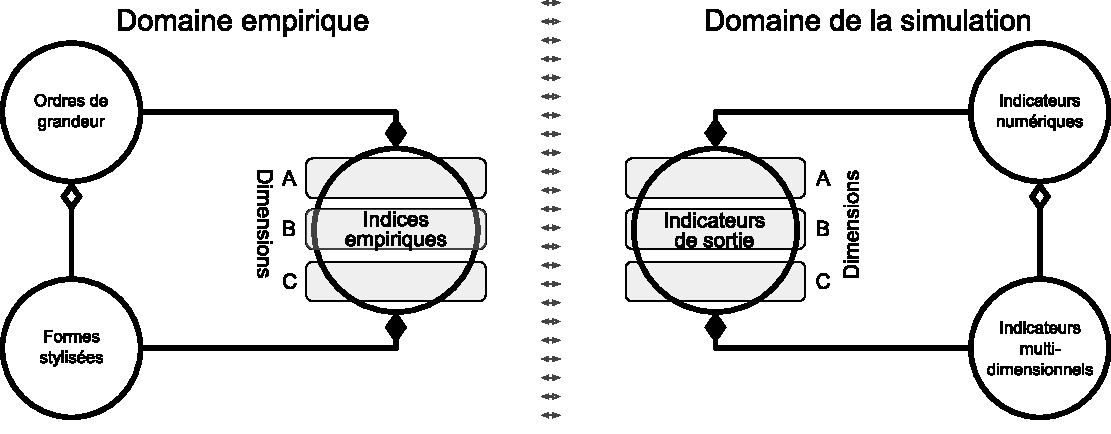
\includegraphics[width=\linewidth]{img/schema_indice_indicateur.pdf}
	\caption{Schéma de synthèse des correspondances entre mesures relevant du domaine empirique et mesures issues des simulations pour l'évaluation du modèle SimFeodal.\\
		\todobox{Lena : Paragraphe difficile}
	La correspondance des éléments est représentée par une symétrie axiale, entre d'un côté des \og indices empiriques\fg{} et de l'autre des \og indicateurs de sortie de simulation\fg{}.
		Les losanges pleins désignent une relation de composition :
		un \og indice empirique\fg{} est soit un ordre de grandeur, soit une forme stylisée.
		Les losanges vides indiquent une relation d'agrégation :
		une forme stylisée est une agrégation d'ordres de grandeurs.
		Les dimensions (A à C) regroupent des indices (et les indicateurs qui leur correspondent) qui peuvent être de plusieurs types, et sont elles aussi comparables et en correspondance entre les domaines.
	} 
	\label{fig:schema_indices} 
\end{figure}


\subsubsection{Les indices empiriques}

Afin d’évaluer la capacité du modèle à reproduire un phénomène observé, il est nécessaire de disposer dans le domaine empirique, de \og points de repère\fg{}.
Selon les modèles, ceux-ci peuvent revêtir de multiples formes et relever de l'ensemble des échelles spatiales et temporelles que l'on choisit de mettre en scène dans le modèle.
Leur point commun est qu'ils doivent pouvoir être mesurés, au sens le plus large, c'est-à-dire être en capacité d'être reproduits et comparables avec d'autres mesures.
Dans cette étude, on a décidé de qualifier ces points de repère d'\og\textbf{indices empiriques}\fg{} et de les regrouper en deux catégories basées sur la précision avec laquelle ils peuvent être décrits\footnote{\todobox{Lena : pas compris la note}\\Et non sur la précision de leur connaissance, cf. \cref{sssec:incertitude}}.
La \cref{fig:schema_indices} illustre cette catégorisation entre la première catégorie -- les ordres de grandeur -- et la seconde -- les formes stylisées --.

\paragraph{Ordres de grandeur}
La première catégorie est constituée d'\textbf{ordres de grandeurs} empiriques estimés -- avec une précision plus ou moins importante (\hl{cf. tableau 3 p. 317 du chap. TMD, à reproduire dans chap 2}).
Certaines valeurs empiriques sont ainsi connues, que ce soit d'après des sources primaires ou secondaires, et peuvent ainsi constituer des indices.
Par exemple, on connaît avec quasi-certitude le nombre d'églises paroissiales de la région Touraine en 1100.
D'autres valeurs empiriques sont en revanche issues d'estimations.
Tel est le cas, par exemple, du taux de foyers paysans isolés en fin de période.
Celui-ci ne peut être renseigné par des sources primaires et il a donc été nécessaire de l'estimer à partir de sources secondaires et en menant des extrapolations.
Il est cependant possible de construire des indicateurs de sortie de simulation offrant une correspondance presque exacte de ces différents indices observés ou estimés (cf. \ref{para:correspondance}, \cnameref{para:correspondance}, p. \pageref{para:correspondance}).
Il est dès lors possible de mener une comparaison entre données observées/estimées et données simulées.
Ces ordres de grandeur peuvent ainsi participer à l'évaluation du comportement du modèle simulé.

\paragraph{Faits et formes stylisés}
La seconde catégorie d'indice empirique est moins précise et ne repose pas sur une valeur observable ou estimable, mais plutôt sur la connaissance experte d'un phénomène.
Il s'agit des \og \textbf{faits stylisés}\fg{}\footnotemark{}, rendant davantage compte d'une tendance dans la forme d'une relation ou d'une organisation que les indicateurs.
On fait un large usage de ces faits stylisés en économie, mais aussi en géographie, par exemple quand on qualifie la tendance des systèmes de peuplement à se hiérarchiser.
La valeur de la pente associée à la courbe rang-taille d'un système de villes tend ainsi vers $1$ (\hl{Trouver ref, sans doute Pumain/Saint-Julien}) à mesure que le système évolue et se hiérarchise.
De la même manière, le modèle de transition démographique d'Adolphe Landry est un fait stylisé, énoncé à partir de l'observation de nombreuses récurrences de l'évolution des populations d'un pays en fonction de leurs taux de natalité et de mortalité.
Ces exemples montrent qu'au sein des faits stylisés, il y a une certaine diversité quant à la précision de leurs énoncés :
on peut quantifier précisément la courbe d'une relation rang-taille et l'allure de son évolution dans le temps, \toChange{alors que la courbe logistique}{phrase à reprendre} de la transition démographique nécessite davantage de mesures et est moins précise dans les paramètres de son énoncé.
Dans notre cas d'étude, les faits stylisés sur lesquels on s'appuiera seront des d'une part des \og allures\fg{} de courbes (par exemple l'évolution dans le temps d'un indicateur), d'autre part des formes de répartition spatiale, et enfin des \og allures\fg{} de courbes résultant d'une composition d'ordres de grandeurs.
Nous qualifierons le premier type de \og \textbf{formes stylisées} temporelles\fg{} (courbe logistique estimée pour la polarisation des foyers paysans par exemple), le second type de \og \textbf{formes stylisées} spatiales\fg{} (changement dans la forme d'occupation de l'espace par les agrégats entre le début et la fin de la période par exemple).


Le troisième type, \og \textbf{forme stylisée} organisationelle \fg{}, correspond à une forme repérable dans l'agrégation à l'échelle du système, comme dans l'observation des hiérarchies grâce aux courbes rang-tailles.
Notons que ces formes stylisées relèvent le plus souvent d'une agrégation ou d'une composition d'ordres de grandeurs (comme figuré dans la \cref{fig:schema_indices}) :
l'évolution dans le temps de la population, par exemple, correspond à un vecteur d'ordres de grandeur, c'est-à-dire à une succession de mesures de la quantité de population pour chaque date étudiée.
\Lena{Même dans le cas }{Rendre § plus pédagogique} d'une agrégation spatiale, par exemple quand on observe \Lena{la hiérarchie du système de peuplement}{pas spatial mais organisationnel, autre exemple.}[-20pt], il s'agit d'une agrégation d'ordres de grandeurs :
cette forme stylisée est constituée d'un ensemble d'ordres de grandeurs, les populations de chaque agrégat de \Lena{population.}{Ajouter petites figures pour clarifier cette phrase}[10pt]

\footnotetext{
	Définis ainsi par \autocite{livet2014diversite}: \og 
	Un ``fait stylisé'' est une présentation simplifiée (i.e. taux, ratio ou écart, structure spatiale) d'une régularité empirique sur l'observation de laquelle il y a un large accord.
	Le terme a été popularisé en économie par Nicholas Kaldor (1961).[Les] faits stylisés peuvent être construits de la manière suivante :
	1) en partant du domaine empirique, on identifie des relations saillantes ; 2) on opère quelques simplifications qui permettent d'inclure formellement ces relations dans des modèles ; 3) une fois admis que ces simplifications ne faussent pas trop les choses, on érige ces relations à la fois simplificatrices et formalisables au rang de `` faits stylisés'', dont les concepts théoriques doivent rendre compte.\fg{}
}

\subsubsection{Les indicateurs de sortie de simulation}

%\todobox{Fin des prises en compte des commentaires de Lena le 02/05/2018}

Les ordres de grandeur et formes stylisées évoqués relèvent du domaine empirique, c'est-à-dire qu'on dispose de données ou de connaissances d'experts à leur sujet.
Afin de pouvoir les mobiliser pour évaluer la capacité du modèle à reproduire le phénomène d'intérêt, il est nécessaire de définir des \textbf{indicateurs de sortie} dans le modèle de simulation, c'est-à-dire des variables informatiques que l'on enregistrera durant l'exécution du modèle et que l'on pourra ensuite comparer aux indices empiriques définis.


\paragraph{Définition}
Comme pour les indices empiriques qui sont leurs équivalents dans le domaine empirique, on peut définir les indicateurs de sortie de simulation, en distinguant des formes numériques simples (des scalaires), et des indicateurs plus complexes, multidimensionnels.
Ces derniers sont en effet nécessaire pour pouvoir confronter les sorties du modèle de simulation avec les formes stylisées identifiées dans le domaine empirique.
Chaque indice empirique doit ainsi se voir correspondre, respectivement, un indicateur de sortie (\cref{fig:schema_indices}).

\paragraph{Correspondance entre indicateurs de sortie de simulation et indices empiriques}\label{para:correspondance}

La correspondance entre indicateurs et indices ne correspond pas toujours à une équivalence exacte.
En effet, si certains indicateurs peuvent trouver un équivalent strict dans le domaine empirique-- le nombre de châteaux connus à chaque date a un sens strictement équivalent au nombre de châteaux simulés par le modèle --, d'autres correspondances sont moins directes.

Il peut s'agir de correspondances ayant trait aux mêmes éléments de base et le passage de l'indicateur à l'indice résulte alors d'une simple conversion.
Par exemple, du point de vue empirique, on connaît à peu près les populations de la région étudiée au début et à la fin de la période.
Dans SimFeodal cependant, on ne modélise pas des individus en tant que tels, mais des foyers paysans.
Le nombre de foyers paysans simulé n'est pas directement comparable à la population estimée, mais en supposant une moyenne de 4 ou 5 habitants par foyer paysan, il est possible d'en déduire un nombre d'habitants.

Dans d’autres cas enfin, le décalage entre indicateurs et indices est plus important.
Il s’agit notamment de caractéristiques du système féodal que l’on sait importantes mais pour lesquelles on ne dispose pas de données facilement quantifiables.
La puissance militaire des seigneurs, par exemple, est complexe à quantifier. 
On sait d’après connaissances expertes que la hiérarchie des puissances était forte à l’époque étudiée, majoritairement dominée par deux seigneurs (les comtes de Tours et de Blois) et assortie d’une grande quantité de petits chevaliers.
On sait de plus qu’avec les liens de vassalité, les grands seigneurs disposaient des forces militaires des seigneurs qui leur étaient assujettis.
Dans le domaine empirique on ne dispose pas d’éléments plus précis pour quantifier la puissance militaire des seigneurs.
Dans le domaine du modèle, en revanche, on a défini un indicateur \og proxy\fg{} de cette puissance à partir du nombre de foyers paysans s’acquittant de droits à chaque seigneur. 
De cette manière, on peut observer précisément en sortie de simulation la hiérarchie implicite entre les seigneurs reproduite par le modèle, avec une quantification de leurs puissances respectives.
Ces éléments peuvent être comparés aux connaissances empiriques sur ces rapports de puissance entre les seigneurs à différents moments de l'époque féodale.

Les correspondances entre indicateurs de sortie et indices empiriques sont ainsi de nature multiple, reflétant différents niveaux de proximité entre le concept mobilisé dans le modèle et ce qui est observable dans le domaine empirique :
les châteaux, entités d’intérêt dans le modèle, ont un équivalent direct dans le domaine empirique (il s’agit d’entités facilement observables et des données historiques les concernant sont disponibles) alors que la puissance militaire des seigneurs, élément moteur dans le modèle, a conduit à utiliser une variable dans le modèle pour laquelle on ne dispose pas d’observations empiriques.

La création d'indicateurs de sortie correspondant aux indices empirique permet donc de quantifier une information qui n'est pas forcément aisément quantifiable dans le domaine empirique.

\paragraph{Indicateur composite}

\hlcyan{La forme numérique\footnote{
		\hlcyan{Lena :\\%
			L’articulation des 2 § suivants ne me parait pas évidente.
			Ils me semblent relever de 2 discussions différentes alors qu’ici ils paraissent liés :\\
			D’un côté il y a les indicateurs composites/synthétiques qui sont issus d’une combinaison des indicateurs simples : ok ;\\
			De l’autre il s’agit d’identifier une fonction objectif. Dans les modèles KISS il s’agit souvent d’une variable simple, par exemple la quantité de population.. Alors que « synthétique » dans ton texte semble beaucoup ressembler à « composite »\\
			Est-ce que ce parag KISS fait sens ici ? Cette discussion là devrait peut-être figurer ailleurs ?}
}}
(scalaire ou vectorielle) des indicateurs de sortie permet de trouver des manières plus simples d'évaluer le modèle que d'observer l'ensemble des indicateurs.
Chaque indicateur étant numérique, il devient en effet possible des les combiner au sein d'indicateurs composites, résultant en quelques indicateurs synthétiques permettant une évaluation plus rapide des résultats d'une simulation.
Ces indicateurs composites sont très fréquemment utilisés en statistiques, permettant par exemple de résumer une information multidimensionnelle en un indicateur simple.
L'Indice de Développement Humain (IDH), par exemple, est un indicateur composite dépendant de l'espérance de vie à la naissance, du niveau d'éducation et du niveau de revenu de chacun des pays caractérisés.
On le trouve très souvent utilisé, parce qu'il permet de résumer le niveau de développement d'un pays en agrégeant trois dimensions majeures, l'aspect sanitaire, culturel et économique.

\paragraph{Indicateur synthétique}

En renforçant cette logique de synthèse de plusieurs dimensions, on peut aller plus loin dans la définition d'un unique indicateur, synthétique, permettant d'évaluer la qualité de représentation d'un modèle.
Là aussi, c'est une pratique très fréquente, qui plus est dans le domaine de la simulation informatique en particulier sur des modèles de type \og KISS\fg{} (\hl{ref. à chap 2 là ou ce sera abordé}).
Il s'agit alors de définir une \og fonction objectif\fg{}, ou \og fonction de \textit{fitness}\fg{}, composée d'une pondération des quelques indicateurs composites qui auront été identifiés.
Être en mesure d'évaluer un modèle à l'aide d'un unique indicateur a des avantages majeurs en pratique, puisque cela permet par exemple d'explorer et de paramétrer un modèle de simulation de manière entièrement automatique (\hl{trouver refs dans JASSS, dans Rey ou Schmitt}) puisqu'on peut alors générer une cartographie simple des résultats du modèle en fonction des valeurs de paramètres utilisés.

Ces indicateurs composites et synthétiques résultent d'une quantification des autres indicateurs (excluant donc les formes stylisées qui sont plus libres d'interprétation), et apportent un grand confort dans le paramétrage d'un modèle de simulation.

\paragraph{Quels types d'indicateurs pour SimFeodal ?}

SimFeodal n'est pas adapté à de tels indicateurs :
une large partie des faits stylisés et ordres de grandeur mobilisés proviennent de connaissances expertes, et les thématiciens qui les ont consolidées rechignent à créer de tels indicateurs composites, en ce que cela demande de pondérer précisement l'importance de chacun des indicateurs par rapport aux autres.
Pour pouvoir pondérer cette importance, il faudrait de plus que les différents indicateurs mobilisés présentent le même niveau de certitude et de variabilité dans leurs résultats, ce qui est peu le cas des indices empiriques -- \Lena{et donc des indicateurs de sortie}{Pas forcément. En fait:	La pondération concerne les indicateurs de sortie;	- l’incertitude est relative aux indices empiriques}[-32pt] -- choisis dans le cadre du modèle SimFeodal.

On aurait ainsi pu créer quelques indicateurs \hlcyan{synthétiques\footnote{
	\hlcyan{Lena:\\Ou composites ?}
}}, mais ceux-ci \hlcyan{ne prendraient en compte qu'une faible proportion du comportement attendu du modèle, résultant en une forte perte du pouvoir explicatif attendu du modèle\footnote{
	\hlcyan{Lena:\\Pas sure de comprendre...\\ En fait il est difficile de créer ces indicateurs si les thématiciens ne peuvent fournir une pondération qui fasse sens pour eux. La combinaison des variables ne fait simplement pas sens pour eux. C’est plutôt cela le pb non ?}
}}.
Par exemple, pour caractériser la polarisation du système de peuplement, il pourrait suffit de définir un indicateur composite fonction du niveau de concentration -- le taux de foyers paysans dispersés --, du nombre de pôles et de l'espacement moyen entre les agrégats.
Les valeurs de l'indicateur généré pourraient renseigner efficacement sur la capacité d'un ensemble de valeurs de paramètres à reproduire le phénomène de polarisation attendu.
Cette information serait cependant grossière, dans la mesure où seraient agrégées dans le groupe des \og simulations réussies\fg{} des configurations extrêmement diverses.
L'information fournie risquerait alors d'être très éloignée des connaissances empiriques des thématiciens :
une information multivariée ne peut pas toujours être résumée, en gardant tout son sens, par une seule variable (de manière univariée).

On a donc fait le choix d'évaluer SimFeodal en conservant des indicateurs de sortie non composites.
Ce choix implique toutefois un problème majeur dans l'analyse des sorties de simulation auquel la réduction de dimensionnalité est \Lena{une réponse}{On a l’impression que tu viens d’expliquer que ce n’est pas intéressant ! Revoir cette formulation donc $\ddot\smile$}[-30pt] :
il est plus simple d'analyser quelques indicateurs plutôt qu'un grand nombre d'entre eux.

\clearpage

\subsection{Hiérarchiser et catégoriser les indicateurs}

SimFeodal s'appuie sur une dizaine d'indicateurs numériques, ainsi que sur plus d'une trentaine d'indicateurs multidimensionnels.
Tous ces indicateurs ne présentent pas le même degré de certitude, la même échelle d'observation, et surtout, le même niveau de précision sur les phénomènes modélisés.
A chaque changement dans le modèle, pour une évaluation complète de la capacité de cette version à reproduire les indices empiriques, il faudrait donc observer et analyser chacun de ces nombreux et divers indicateurs.
Dans le contexte du paramétrage d'un modèle s'appuyant sur une logique itérative et incrémentielle (voir \cref{enc:construction-indicateurs}), on imagine bien que cela n'est pas possible :
le nombre d'indicateurs est bien trop élevé pour avoir rapidement une vision globale de la qualité de représentation du modèle.
Il faut dès lors, comme pour toute analyse synthétique, concevoir une hiérarchie d'observation et d'utilisation des indicateurs :
il ne sera pas nécessaire d'analyser chacun des indicateurs dans la plupart des cas, seuls les indicateurs jugés plus importants pourront être analysés.
Les indicateurs de moindre importance ne seront mobilisés que pour départager des situations dont la différence ne serait pas suffisament explicitée par l'usage des indicateurs principaux.

\subsubsection{Incertitude}\label{sssec:incertitude}
Dans le modèle de simulation, les indicateurs de sortie sont à analyser en tenant compte de la précision des indices qu'ils représentent.
Il ne faudra ainsi pas étudier la croissance  du nombre d'agrégats au cours de la simulation de manière fine, par exemple en étudiant le coefficient directeur de la courbe, quand l'empirie ne donne quasiment aucune information à ce sujet si ce n'est qu'il y a bien plus d'agrégats en fin de période qu'au début.
On peut vouloir quantifier la précision de ces données, par exemple à l'aide des méthodes développées dans le champ des observations floues et/ou incertaines (voir par exemple le travail de Cyril de Runz sur les données \og imparfaites\fg{} \autocite{de2008imperfection}).
Cette quantification de l'incertitude pourrait alors servir de base à l'établissement d'une hiérarchie des indicateurs :
on analyserait en premier lieu l'écart entre les ordres de grandeurs empiriques bien connus (\hl{cf. tableau du niveau de certitude des objectifs}) et les indicateurs calculés sur les données simulées.
Les ordres de grandeur plus incertains seraient analysés dans un second temps (augmentation de la charge fiscale entre 800 et 1100 par exemple), et les formes stylisées viendraient enfin clore cette hiérarchie d'indicateurs.
Toutefois, SimFeodal se caractérise d'une part par une très forte hétérogénéité dans les niveaux de connaissance des ordres de grandeurs et faits stylisés modélisés, et d'autre part, se voulant un modèle théorique (\hl{A dire spécifiquement dans le chapitre 2; y faire une ref ici}), il n'y a pas d'obligation de \og coller aux données\fg{} à tout prix :
la vraisemblance d'ensemble du modèle compte bien plus que la précision de chacune de ses composantes.


\subsubsection{Catégoriser les indicateurs : définir des dimensions d'analyse}
En présence de plus d'une quarantaine d'indicateurs, il est toutefois nécessaire, a minima, d'organiser leur analyse.
On a vu qu'il n'était pas justifié de mener cet ordonnancement à partir des propriétés intrinsèques des indicateurs du modèle.
Au contraire, et cela porte bien plus de sens vis-à-vis du rôle d'un modèle, la hiérarchisation des sortie du modèle doit suivre la hiérarchie implicite qui structure les hypothèses et objectifs du modèle en lui-même.
Ces hypothèses et objectifs sont multiples dans SimFeodal, et dès lors, une hiérarchie globale ne peut être définie.
Il convient donc de catégoriser les indices empiriques -- et les indicateurs de sortie de simulation leur correspondant --, avant d'organiser, au sein même de ces catégories, les indices les caractérisant.
La hiérarchisation des indicateurs se fera donc relativement à chacune de ces catégories.

Dans le chapitre précédent (\hl{ref chap 2}), nous présentions les principales dynamiques à reproduire avec le modèle SimFeodal :
(1) polarisation, (2) hiérarchisation et (3) fixation des foyers paysans.
En postulant que ces dynamiques sont caractéristiques du modèle, on peut s'appuyer sur cette triade pour caractériser les sorties du modèle,c'est-à-dire mener la confrontation entre indices empiriques et indicateurs de sortie.
En reprenant ces catégories, que l'on nommera \textbf{dimensions} (voir \cref{fig:schema_indices}), on va donc répartir chacun des indicateurs dans la dimension qu'il sera le mieux en mesure de décrire.
Cette répartition n'a pas à être égale, chaque dimension pouvant s'appuyer sur un nombre différent d'indicateurs.
De même, chaque dimension sera composée d'indicateurs dotés d'une qualité de représentation ou d'un niveau de certitude hétérogène.
Le seul point commun des indicateurs de sortie de chaque dimension doit être thématique.
Les trois dimensions choisies -- polarisation, hiérarchisation et fixation --, et les indicateurs qui les caractérisent dans le modèle, sont dès lors considérés comme les trois dimensions d'analyse des sorties de SimFeodal.

\subsubsection{Hiérarchiser les indicateurs dans chaque dimension}\label{par:hierarchie_interne}
Chacune de ces dimensions s'applique à plusieurs types d'agents du modèle.
Pour définir la hiérarchie interne aux dimensions, on retiendra les agents les plus impactés par les dynamiques correspondant à ces dimensions :
la polarisation, par exemple, peut être observé depuis le point de vue de ce qui polarise (les attracteurs) tout autant que de ce qui est polarisé (les foyers paysans).
On aura alors tendance à examiner d'abord un indicateur de sortie caractéristique mono-dimensionnel, caractéristique de la structure dans son ensemble à son état final.
Les indicateurs de sortie représentatifs des dynamiques, par exemple les indicateurs multi-dimensionnels, ayant mené à cette structure finale, seront étudiés dans un second temps.
Dans cet exemple, on analysera donc d'abord le résultat effectif de la polarisation, c'est-à-dire la concentration des foyers paysans en agrégats, avant d'observer la répartition et les diversité des attracteurs ayant entrainé ce phénomène.
On peut dès lors définir des \og indicateurs principaux\fg{} pour chaque dimension, représentatifs des grands traits des structures auxquelles on souhaite aboutir en sortie de simulation, et des \og indicateurs secondaires\fg{}, permettant d'affiner l'évaluation de chacune de ces dimensions.

\subsubsection{Une hiérarchie mouvante}
Notons que l'analyse des indicateurs de sortie suit une hiérarchie parfois mouvante, et en tous les cas, assez peu quantifiable :
si l'ordre d'observation est plutôt stable, l'importance que l'on portera à chacun des indicateurs peut varier.
Les indicateurs principaux de chaque dynamique sont ainsi \og incontournables\fg{}, c'est-à-dire qu'un résultat trop loin de celui des indices empiriques est disqualifiant.
Parmi les indicateurs secondaires, il n'est pas toujours possible, d'après les connaissances des experts sur le sujet, d'établir une priorité ou une pondération de chaque indicateur.
L'évaluation de la polarisation par exemple (\cpageref{subsub:polarisation}), se définit principalement par rapport à un indicateur principal -- le taux de foyers paysans dispersés --, mais selon les résultats des autres indicateurs de sortie, on leur attribuera une importance variable.
L'étude de la dispersion des agrégats et pôles peut ainsi se révéler plus importante que celle de l'évolution du nombre d'agrégats selon les paramètres que l'on souhaite ajuster, ou se montrer tout au moins plus différenciante selon l'état du paramétrage.


\begin{encadre}{Incrémentalité des indicateurs}{construction-indicateurs}
	De la même manière que les paramètres et mécanismes d'un modèle de simulation tendent à évoluer\footnotemark{} au cours du temps de la construction, souvent afin d'affiner un comportement observé, les indicateurs de sortie sont amenés à évoluer aussi.
	
	Ainsi, en cas de modifications fines du modèle, il est fréquent que les indicateurs initialement choisis ne suffisent plus à départager des versions du modèle quant à un phénomène spécifique.
	Par exemple, quand on observe le phénomène de polarisation dans les sorties de SimFeodal, l'indicateur du nombre d'agrégats est extrêmement synthétique et informatif jusqu'à ce que l'objectif soit atteint ou que les modifications ne parviennent plus à le faire évoluer.
	À partir de ce moment, afin d'améliorer la vraisemblance de la situation simulée par le modèle, on peut se focaliser sur la distribution spatiale de ces agrégats, par exemple pour vérifier qu'ils sont bien répartis de manière homogène dans l'espace, et non trop concentrés.
	
	L'observation de la répartition spatiale requiert certes de nouvelles analyses, mais surtout, par exemple, d'enregistrer les positions des agrégats au cours du temps.
	Si cet indicateur de sortie n'était pas utile avant cela, il n'y avait aucun interêt à l'enregistrer.
	Il faut donc adapter l'implémentation du modèle pour générer, faire évoluer et enregistrer une nouvelle variable informatique correspondant à cet indicateur.
	Dès lors, on pourra composer un nouvel indicateur synthétique, qui, dans cet exemple, pourrait prendre la forme d'un indice de concentration spatiale).
	
	Ce procédé incrémental dans la construction des indicateurs est très fréquent, mais pose toutefois un problème majeur :
	sauf à adapter chacune des anciennes versions du modèle implémenté pour y ajouter l'enregistrement des nouveaux indicateurs nécessaires, on ne pourra rendre strictement comparable les sorties de toutes les itérations du modèles informatique.
	Et même alors, il faudrait ré-executer des réplications de chaque version du modèle implementé à chaque ajout d'indicateur, quand bien même les indicateurs présent initialement étaient jugés suffisants.
	Un dernier obstacle est plus gênant :
	certains indicateurs sont spécifiques à des mécanismes, et en cas de changement de ces derniers, ils peuvent ne plus être calculables ou simplement comparables.
	Par exemple, des versions antérieures du modèle enregistraient les comportements individuels des foyers paysans quant à leur \og choix\fg{} de déplacement, selon qu'ils étaient à l'origine localisés dans un agrégat ou dispersés.
	Une simplification du modèle a abouti à la modification des règles différenciant les possibilités de déplacement :
	on n'observe plus si le foyer paysan est dans un agrégat, mais plutôt s'il est dans un agrégat doté d'un pôle d'attraction.
	Dès lors, les analyses basées sur les choix de déplacement des foyers paysans selon leur origine ne sont plus comparables avec celles des versions antérieures au changement dans le modèle, quels que soient les détails d'implémentation de ce dernier.
	
	Ces éléments expliquent que dans les résultats de chaque étape du paramétrage du modèle, on ne présente pas systématiquement l'ensemble des indicateurs, y compris quand ceux-ci pourraient être plus pertinents que les indicateurs présentés.
\end{encadre}
\footnotetext{De manière incrémentielle et itérative, voir \hl{dans le chapitre x?} et http://itsadeliverything.com/revisiting-the-iterative-incremental-mona-lisa}


\pagebreak

\section{Les indicateurs et dimensions de SimFeodal}

\subsection{Évaluer la polarisation des foyers paysans \label{subsub:polarisation}}

La polarisation des foyers paysans dans l'espace du modèle est sans doute la dimension principale des dynamiques spatiales que l'on cherche à reproduire.
Rappelons ici que l'on estime, à partir des connaissances d'experts, que les foyers paysans sont très majoritairement dispersés en 800, et concentrés au sein de villages et petites villes en 1100.
Le modèle cherche à reproduire cette polarisation, par le biais d'une concentration des foyers paysans, initialement localisés aléatoirement dans l'espace mais n'en parsemant qu'une faible part, en des agrégats de foyers paysans répartis dans dans une plus large partie de l'espace modélisé.
\todobox{Mettre un schéma pour rendre compréhensible cette contradiction apparente.}

Pour analyser la polarisation du système de peuplement, il est nécessaire de définir des indices permettant de caractériser ce phénomène.
Ces indices doivent d'une part avoir une logique thématique, c'est-à-dire être appropriés à la description et à l'étude de la polarisation, mais doivent  pouvoir être produits et enregistrés dans le modèle de simulation, formant des indicateurs.

Pour l'étude de la polarisation, il est nécessaire de faire appel à des indices hétérogènes, chacun devant être en mesure de décrire les différents aspects du phénomène de polarisation.
En conséquence, on a choisi de faire appel à plusieurs indicateurs qui doivent permettre d'étudier aussi bien l'aspect structurel du système simulé en son état final que la forme et la tendance que prennent les changements qu'il subit.

L'indicateur principal est le taux de dispersion des foyers paysans.
Si celui-ci est trop important (c'est-à-dire très supérieur aux valeurs estimées empiriquement), cela signifie que la polarisation générée par le modèle est insuffisante, et dès lors, obligatoirement insatisfaisante.
A contrario, une valeur trop faible serait symptomatique d'un emballement des mécanismes simulés, figeant la situation dans une concentration absolue des foyers paysans, ne laissant dès lors plus de place à la diversification des situations locales et de la hiérarchisation d'ensemble.

Pour affiner ce constat, on fait appel à d'autres indicateurs :
le nombre d'agrégats, de pôles, ou encore la dispersion spatiale de ces deux types d'entités.
Ces indicateurs ne permettent pas, à eux seuls, de caractériser le succès de la dynamique de polarisation modélisée, mais ils aident à affiner l'analyse de cette dynamique telle que produite par le modèle de simulation.
Ils éclairent ainsi le phénomène de polarisation sous des angles légèrement différents, ayant plus pour objet de diagnostiquer les problèmes potentiels qui mèneraient à une mauvaise polarisation plutôt que de qualifier celle-ci.
Par exemple, la dispersion des agrégats et pôles peut renseigner, une fois le taux de foyers paysans dispersé jugé trop important, sur une des raisons probables de ce résultat non satisfaisant.
Il s'agit donc d'indicateurs secondaires, permettant de préciser la capacité du modèle à reproduire les faits stylisés, alors que l'évaluation de cette capacité est surtout le rôle de l'indicateur principal.


\subsubsection{Taux de foyers paysans dispersés}

Cet indicateur, et sa déclinaison temporelle, sont vraisemblablement les plus évidents :
plus le taux de foyers paysans dispersés en fin de simulation est faible, plus le système de peuplement est polarisé.
On a vu \footnote{\hl{Ne pas oublier de présenter les objectifs dans chapitre 2. Ou alors, on les présente ici au fur et à mesure qu'on mentionne les indicateurs}} qu'empiriquement, autour de 1160, on observe environ $20\%$ de foyers paysans encore dispersés, alors qu'ils sont près de $95\%$ au départ.
Le modèle sera donc d'autant plus satisfaisant que cet indicateur s'approchera de $20\%$ en fin de simulation.

La \og déclinaison temporelle\fg{} mentionnée juste au dessus permet d'affiner légèrement la précision de l'information communiquée par cet indicateur :
il faut certes atteindre un objectif quantifié ($20\%$), mais les hypothèses empiriques permettent aussi de penser qu'il faut que l'évolution de cet indicateur au cours du temps présente une tendance stable à la diminution
%(
%\begin{sparkline}{5}
%	\spark 0 .995 .25 0.8 .5 0.6 .75 0.4 1 .2 /
%\end{sparkline}
%)
, diminuant ainsi plus ou moins, avec de faibles fluctuations à chaque pas de temps.
Une configuration de paramètres présentant des valeurs d'indicateurs en sortie proches des objectifs en fin de simulation mais fluctuant fortement pendant son déroulement ne sera ainsi pas valide.
Elle montrerait en effet  un phénomène trop aléatoire au cours du temps, dont on ne peux penser qu'il s'est déroulé historiquement selon les dires d'experts qui considèrent que cette évolution s'est déroulée de manière continue dans le temps.

\begin{mdframed}[backgroundcolor=gray!10,footnoteinside=false]
	
	Dans la version 0 de SimFeodal, on atteint en moyenne (moyenne des réplications) $\textbf{57\%}$ de foyers paysans isolés en fin de simulation.
	C'est un taux bien plus important que les $20\%$ attendus, illustrant dès lors une polarisation trop faible.
	Dans la première moitiée de la période (jusqu'en 1000, (\cref{fig:taux-isoles-v0})), le taux est en diminution constante et linéaire, ce qui est une bonne tendance, et ne présente de plus presque pas de variabilité, ce qui l'est aussi.
	Pourtant, à partir de 1000, la variabilité augmente, et le la diminution du taux au cours du temps s'interrompt, avant de prendre une allure croissante.
	L'allure de la courbe sur la seconde moitié de la simulation est donc très éloignée de ce qui est attendu au regard des connaissances empiriques, aussi bien en matière de tendance qu'à la vue du taux décevant atteint au final.
\end{mdframed}

\begin{figure}[H]
	\captionsetup{width=\linewidth}
	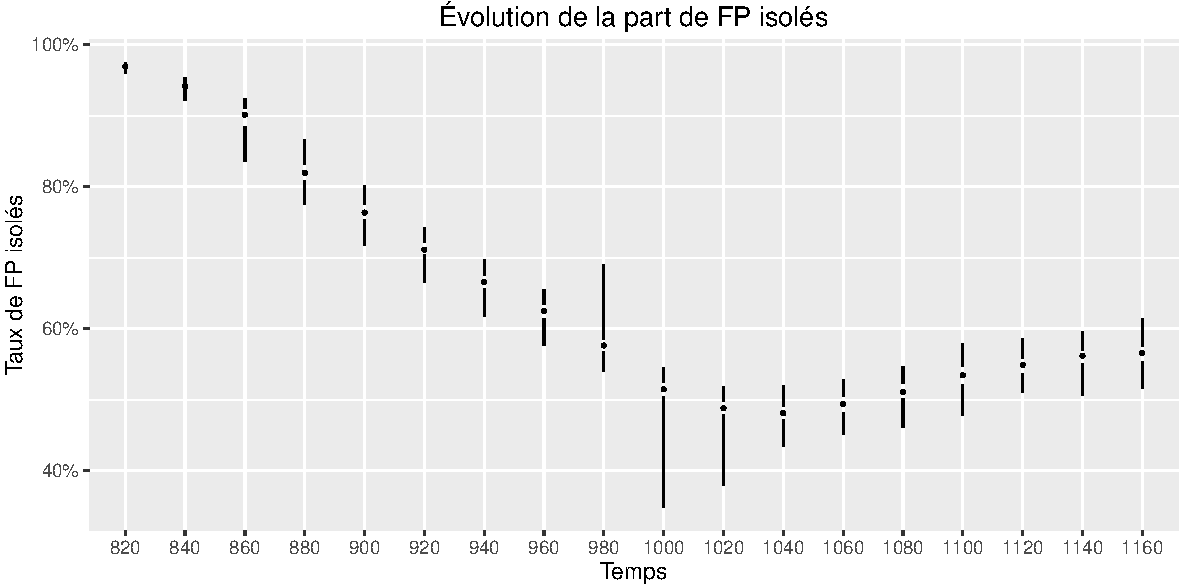
\includegraphics[width=\linewidth]{img/resultats/v0_taux_FP_isoles.pdf}
	\caption{Évolution de la part des foyers paysans isolés.} 
	\label{fig:taux-isoles-v0} 
\end{figure}

\clearpage

\subsubsection{Nombre d'agrégats}

Puisque les foyers paysans se concentrent au sein d'agrégats, il est logique d'observer l'évolution de ces derniers.
Là aussi, (\hl{objectif à définir}), on peut considérer qu'un nombre d'agrégats en fin de simulation proche de l'objectif, $200$, permet de caractériser une polarisation réussie.
Cet indicateur ne peut être lu seul, et c'est pour cela qu'il vient dans un second temps (cf. \ref{par:hierarchie_interne}, \cnameref{par:hierarchie_interne}, p.\pageref{par:hierarchie_interne}) :
en effet, un faible nombre d'agrégats peut aussi bien être révélateur d'une très faible polarisation des foyers paysans (ceux-ci restant dispersés) que d'une trop importante (un unique agrégat concentrant l'ensemble des foyers paysans par exemple).
Une fois le taux de foyers paysans dispersés connu et ces potentiels biais pris en compte, le nombre d'agrégats et son évolution nous renseigne cependant sur les dynamiques de polarisation.
D'après les connaissances expertes, on s'attend à ce que le nombre d'agrégats, très faible au départ (24 dans la version 0), suive trois phases :
une première phase de croissante lente, le temps que les mécanismes agissent sur la polarisation, suivie d'une période de croissance plus rapide, une fois que tous les foyers paysans commenceront à être suffisament attirés par les pôles pour y former des agrégats, et enfin, une nouvelle phase de croissante plus lente, une fois les foyers paysans répartis dans les agrégats existants et qui se déplaceront vers des agrégats plus importants, hiérarchisant le système de peuplement.
Cette allure d'évolution rappelle les fonctions logistiques connues par exemple pour les cycles de diffusion/adoption des innovations \hl{ref Pumain ou MN Comin}, et résulte des connaissances expertes des archéologues spécialistes de la période.

\begin{mdframed}[backgroundcolor=gray!10,footnoteinside=false]
	Le nombre d'agrégats est assez satisfaisant dans la version 0 du modèle.
	Il s'élève ainsi à $\textbf{187}$ en moyenne, cette dernière étant d'ailleurs stable au regard des réplications.
	L'écart à l'objectif ($200$) est donc assez minime.
	On a toutefois vu que le taux de foyers paysans isolé était bien trop important, et dès lors, ces agrégats sont logiquement composés de trop peu de foyers paysans.
	
	L'observation de cet indicateur au cours du temps (\cref{fig:nombre-agregats-v0}) est quant à elle assez satisfaisante :
	on retrouve bien les trois phases attendues, quand bien même le début de la croissance plus importante (vers 1000 ici) est un peu trop tardive.
	Ce moment coïncide de plus avec la stagnation puis l'inversion de la courbe d'évolution de la part de foyers paysans isolés.
	
	On peut quand même considérer que si la polarisation n'est pas assez importante, les structures qui en résultent semblent correspondre à l'empirie.
\end{mdframed}

\begin{figure}[H]
	\captionsetup{width=\linewidth}
	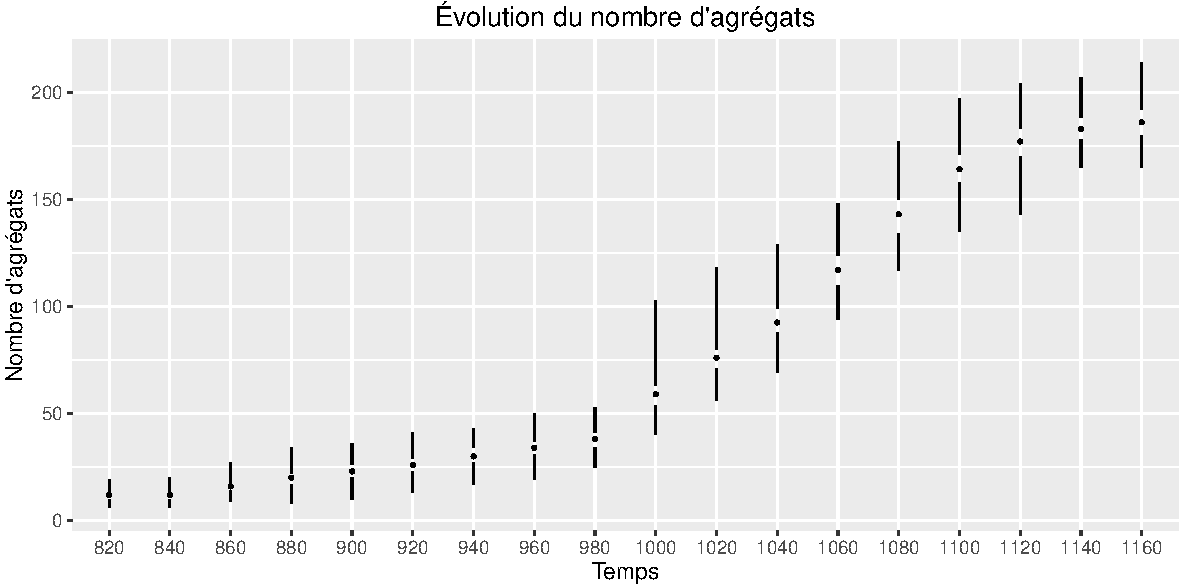
\includegraphics[width=0.5\linewidth]{img/resultats/v0_nombre_agregats.pdf}
	\caption{Évolution du nombre d'agrégats.} 
	\label{fig:nombre-agregats-v0} 
\end{figure}

\todobox{
	Il y a un problème ici par rapport à ce qui a été mis dans le chapitre :
	dans le chapitre TMD, on mentionne 83 agrégats en moyenne, alors que dans l'analyse de Base, il y en a 187...
}	

\clearpage

\subsubsection{Nombre de pôles}\label{para:nb-poles}

Dans le modèle SimFeodal, les foyers paysans sont polarisés par des pôles d'attraction.
Pour une polarisation efficace, il est donc nécessaire que les pôles soient suffisamment nombreux, c'est-à-dire, \textit{a minima}, autant que d'agrégats attendus ($200$).
Contrairement aux agrégats, un nombre trop important de pôles ne constitue pas un problème :
en considérant que $20\%$ des foyers paysans doivent demeurer isolés en fin de simulation, il est vraisemblable qu'une partie des pôles, par exemple composés d'une église paroissiale, n'aient pas vocation à voir la constitution d'un agrégat autour d'eux.

Par ailleurs, afin de renforcer la polarisation par l'action de l'attraction différenciée -- selon le nombre de foyers paysans contenus dans chaque agrégat\footnote{\label{ftn:preferential-attachment}
	L'attraction qu'exercent les pôles contenant des agrégats de population est ainsi plus forte lorsque ces derniers sont constitués d'un nombre de foyers paysans important, et moindre quand ce nombre est faible.
	Cela place ce mécanisme dans une logique proche de celle de l'attachement préférentiel identifié par \autocite{yule1925ii} et  \autocite{simon1955class}, cités par \autocite[93]{schmitt_modelisation_2014}) \label{ftn:attachement-preferentiel}
} --, il faut que le taux de pôles contenant un agrégat soit important, et surtout croissant au cours du temps :
comme dans l'empirie, cela est alors le marqueur que de petits pôles d'attractions, comme les églises paroissiales, parviennent à polariser suffisament de foyers paysans de leur voisinage pour aboutir à la création d'un petit agrégat, un village par exemple.

Pour un résultat satisfaisant, il faut donc que le nombre de pôles augmente régulièrement au cours de la durée de la simulation, et que le taux de pôles contenant un agrégat augmente lui aussi de manière continue.

\begin{mdframed}[backgroundcolor=gray!10,footnoteinside=false]
	L'évolution du nombre de pôles est assez représentative de l'empirie dans la version 0 de SimFeodal.
	On aboutit ainsi sur $\textbf{190}$ pôles en moyenne en fin de simulation, ce qui est dans le bon ordre de grandeur, quoi qu'un peu trop faible.
	Ce nombre est en croissance constante à partir de 940 (\cref{fig:nombre-poles-v0}).
	Ce départ quelque peu tardif peut expliquer le relatif manque de pôles en fin de simulation.
	
	L'analyse de la constitution de ces pôles en matière d'agrégat est toutefois plus décevante :
	la croissance n'est pas linéaire, stagnant entre 940 et 1000, puis à partir de 1040.
	On constate ici un mauvais comportement du modèle par rapport à l'empirie :
	il y a création de nombreux pôles, mais ceux-ci ne suffisent pas à polariser les foyers paysans.
	On peut donc penser qu'il s'agit de nombreux pôles ruraux, par exemple composés d'une unique église paroissiale, ne suffisant dès lors pas à concentrer les foyers paysans alentours.
	
	Dans cette dimension, comme pour l'indicateur principal qu'en est le taux de foyers paysans dispersé, l'effet de la polarisation apparaît nettement trop faible.
\end{mdframed}


\begin{figure}[H]
	\captionsetup{width=\linewidth}
	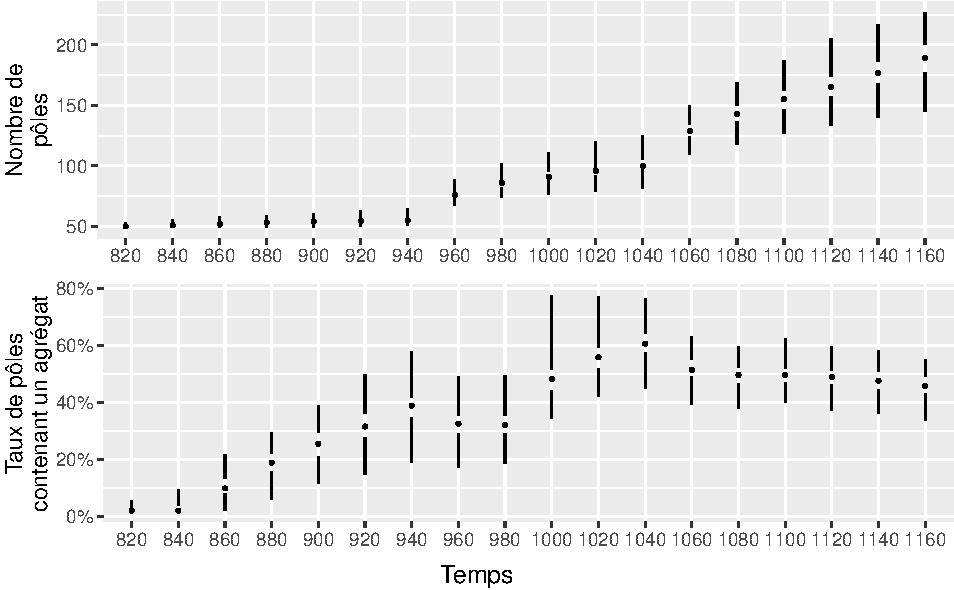
\includegraphics[width=0.5\linewidth]{img/resultats/v0_nombre_poles.pdf}
	\caption{Évolution du nombre de pôles et du taux de pôles contenant un agrégat.} 
	\label{fig:nombre-poles-v0} 
\end{figure}

\clearpage

\subsubsection{Dispersion des agrégats et pôles}\label{par:polarisation-dispersion}

Les indicateurs présentés ci-dessus avaient en commun d'être des indicateurs de sortie, générés automatiquement, et présentés sous forme d'agrégations des réplications.
Pour préciser l'analyse de la polarisation, il est toutefois nécessaire d'aborder une dimension qui n'est fondamentalement pas agrégeable dans les indicateurs de sortie :
l'espace du modèle.
Comme celui-ci est théorique et aléatoire, il n'y a aucun sens à agréger des entités différentes, par exemple des agrégats, sachant que ceux-ci occupent des localisation aléatoires et ne sont pas identifiables en tant que tels.

On ne peut cependant pas se passer d'une analyse spatiale de la répartition des pôles et agrégats afin de comprendre les dynamiques effectivement simulées par le modèle.
La distribution spatiale des agrégats et des pôles est en effet un facteur majeur de la polarisation :
s'ils sont très concentrés, les foyers paysans non présents alentours ne trouveront pas d'attracteurs à proximité, et ne seront de plus pas particulièrement affectés par l'augmentation des droits (banaux etc.) et des contraintes spatiales (proximité à une église, à un château etc.).
A l'inverse, des agrégats entièrement dispersés ne favoriseraient pas la structure spatiale hiérarchisée que l'on chercher à faire émerger.

Afin que le comportement du modèle soit satisfaisant, il faut donc que les pôles et agrégats occupent l'ensemble de l'espace du modèle, tout en présentant des zones de concentration relatives plus importantes.
Comme on ne peut agréger les représentations spatiales, il convient, pour cette analyse, de regarder individuellement un échantillon de configurations spatiales générées.

\begin{mdframed}[backgroundcolor=gray!10,footnoteinside=false]
	La lecture des cartes de répartition des agrégats et des pôles de deux réplications de la version 0 (\cref{fig:cartes-agregats-v0}) va, dans l'ensemble, dans le sens de l'empirie.
	On peut ainsi remarquer que ces entités ont bien tendance, au cours du temps, à se disperser dans l'espace modélisé.
	En fin de simulation, tout l'espace est occupé, et on remarque même que certaines zones voient une forte concentration en agrégats, reproduisant les faits stylisés connus.
	La répartition spatiale des agrégats -- et des pôles -- est donc bonne, et ne semble pas opposer d'obstacle à la polarisation attendue du système de peuplement.
	
	Ce résultat peut cependant être nuancé par l'observation de la dynamique de cette dispersion :
	on constate ainsi que la dispersion s'effectue rapidement (entre 800 et 940), et n'évolue plus vraiment après.
	Ce phénomène est donc plus rapide dans cette version 0 du modèle que dans les connaissances empiriques de la région Touraine.
	
	On peut enfin remarquer, en préalable aux dynamiques de hiérarchisation du système que l'on s'apprête à étudier, que ces sorties illustrent un manque criant de hiérarchie quant à la composition des agrégats :
	on ne remarque, visuellement, que peu de différence entre les agrégats, et surtout, cette hiérarchie semble faiblir entre 1040 et 1160 (les agrégats les plus importants ont vu leur nombre de foyers paysans diminuer).
\end{mdframed}

\begin{figure}[H]
	\captionsetup{width=\linewidth}
	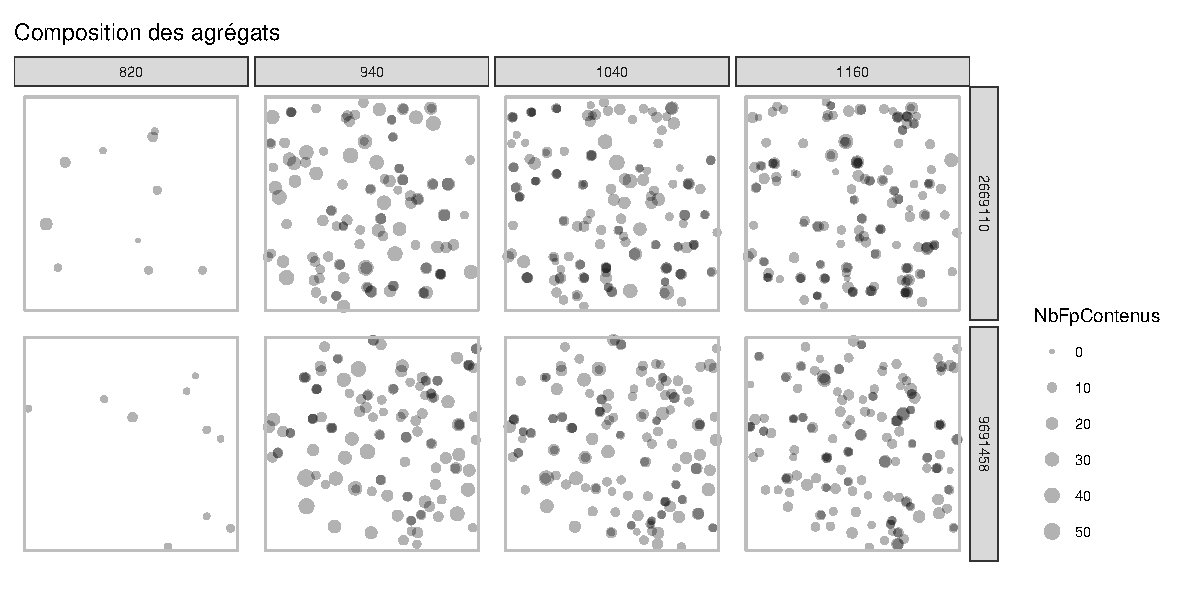
\includegraphics[width=\linewidth]{img/resultats/v0_cartes_agregats.pdf}
	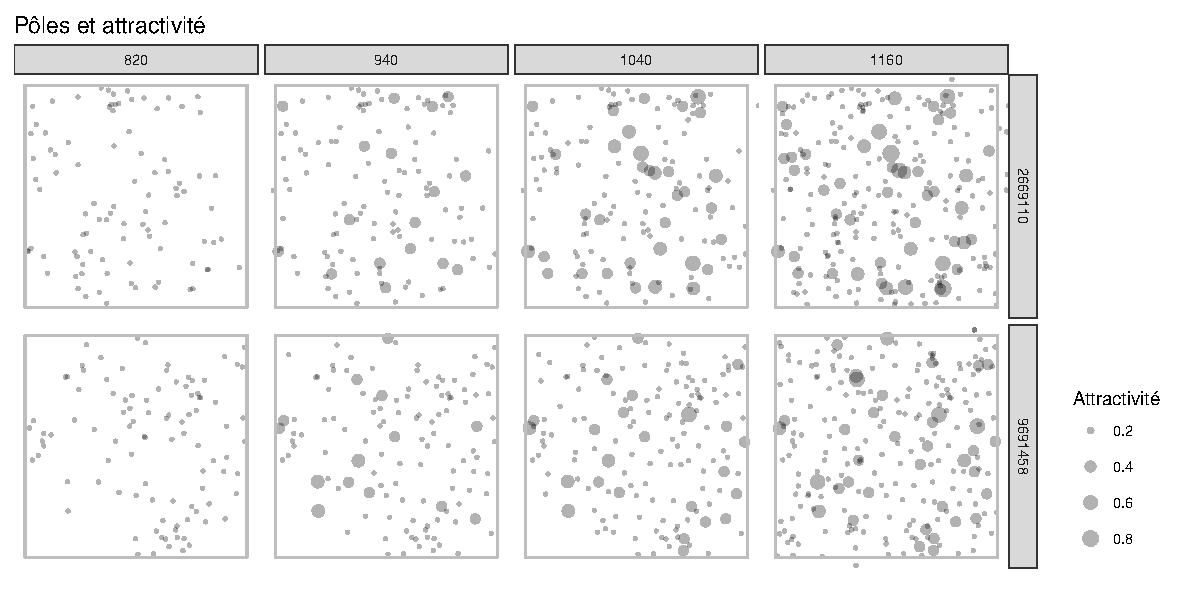
\includegraphics[width=\linewidth]{img/resultats/v0_cartes_poles.pdf}
	\caption{Évolution de la répartition spatiale des agrégats et pôles, pour deux réplications.} 
	\label{fig:cartes-agregats-v0} 
\end{figure}

\clearpage

\subsection{Évaluer la hiérarchisation du système de peuplement}

La seconde dimension de l'évaluation du modèle SimFeodal correspond à l'étude de la hiérarchisation du système de peuplement.
On déduit en effet des connaissances empiriques une forte hiérarchisation du système de peuplement sur la période, et plus généralement, des entités présentes.
On passe ainsi, en 800, d'un habitat dispersé dans lequel coexistent quelques agrégats de taille uniforme, à un habitat concentré dans des agrégats de taille très hétérogènes à la fin du XIIème siècle.
La distribution des tailles des agrégats est estimée par les connaissances expertes, toutes proportions gardées, comme assez proche des distributions observées aujourd'hui dans les systèmes de peuplement.
On souhaite ainsi que les agrégats modélisés suivent une distribution approchant la distribution log-normale.

Par extension, et là encore d'après les connaissances thématiques, l'ensemble des entités doit aussi suivre le même type de forme.
Par exemple, les pôles, tant en terme d'attractivité que de composition, doivent aussi montrer une hiérarchie du même ordre, ainsi que les seigneurs -- à travers leur puissance, au moins pour les petits seigneurs --, ou encore les paroisses, par le nombre de paroissiens qu'elles desservent.

Comme pour l'étude de la polarisation, on peut définir un indicateur principal de cette hiérarchisation du système de peuplement :
la forme de la distribution de la composition en foyers paysans des agrégats.

De la même manière que pour la polarisation, les indicateurs secondaires ont aussi pour but de préciser cet indicateur principal, et en particulier d'analyser les moteurs de cette hiérarchisation du peuplement.
On a en effet choisi d'observer plutôt la hiérarchisation des autres types d'entités -- pôles, seigneurs, paroisses --, pour vérifier qu'elles accompagnent et/ou entraînent bien la hiérarchisation des agrégats.
La hiérarchie des pôles, par exemple, a une influence directe sur l'attraction effectuée sur les foyers paysans (polarisation) et sur la hiérarchisation des agrégats :
par effet d'attraction différenciée (voir la note de bas de page \ref{ftn:attachement-preferentiel} \cpageref{ftn:attachement-preferentiel}), des agrégats plus importants se constituemouvementnt autour des pôles les plus importants.

Comme pour la polarisation, l'analyse de la capacité du modèle a reproduire la hiérarchisation du système de peuplement se fait donc en deux temps :
en premier lieu, on évalue cette capacité à l'aide de l'indicateur principal, puis on précise cette qualification et on essaie de l'expliquer à l'aide des indicateurs secondaires.


\subsubsection{Hiérarchie des agrégats}

L'indicateur principal est un indicateur agrégé, correspondant à la forme de la distribution des agrégats mesurés par le nombre de foyers paysans qui les composent.
Cet indicateur est classique dans l'analyse des systèmes de peuplement, et il est courant de l'observer par le biais d'un indicateur agrégé simple, correspondant à la loi rang-taille.
On observe pour cela le modèle statistique, ou sa représentation graphique tout du moins, mettant en relation le logarithme de la taille des individus (le nombre de foyers paysans composant chaque agrégat ici) et le logarithme du rang de cet individu.
Comme pour toute régression linéaire, on peut alors quantifier l'ajustement du modèle grâce au coefficient de détermination ($R^2$), et spécifier la pente de la courbe, représentant le degré de hiérarchie, à travers le coefficient directeur ($a$ dans la formule $y = ax + b$).

Dans le cas de SimFeodal, le faible nombre d'agrégats ainsi que la variabilité de leurs tailles rend difficile cette analyse quantifiée, le coefficient directeur, par exemple, étant très sensible aux faibles effectifs.
On utilise toutefois la représentation graphique décrite comme un indicateur majeur de la hiérarchie des agrégats.

Du point de vue des connaissances empiriques, la courbe doit ainsi voir sa pente augmenter avec le temps, tout en devenant plus convexe, ce qui représente la \og longue traine\fg{} des petits agrégats, empiriquement observée dans toutes les distributions de systèmes de peuplement.

Avec une autre représentation graphique du même phénomène, en discrétisant les agrégats selon leur taille et en dénombrant le nombre d'agrégats de chaque classe, on peut aussi avoir une vision plus synthétique (car moins exhaustive) de la forme de la distribution.
On doit alors obtenir un nombre décroissant d'agrégats à mesure que la classe représente un nombre élevé de foyers paysans.

\todobox{
	Ça vaudrait peut-être le coup, pour chaque indicateur présenté sous forme graphique (évolution ou forme), de faire un graphique théorique (une sorte de courbe parfaite) de ce que l'on souhaite observer.
}

\begin{mdframed}[backgroundcolor=gray!10,footnoteinside=false]
	La version 0 de SimFeodal présente une hiérarchisation des agrégats nettement trop faible.
	La courbe rang-taille (\cref{fig:rt-agregats-v0}) est ainsi trop faiblement pentue, et présente une forme trop linéaire :
	la convexité due à la longue traine n'est pas assez visible, en raison sans doute de trop faibles valeurs  en haut de la hiérarchie, qui ne \og tire\fg{} alors pas assez la distribution.
	Ce résultat de simulation est d'autant plus perturbant que son évolution est éloignée de l'empirie :
	on remarque en effet que la distribution se hiérarchise bien entre 800 et 1020, présentant à cette date une allure très satisfaisante.
	Pourtant, après cette période, les agrégats voient leur hiérarchie diminuer nettement et les agrégats les plus peuplés diminuer en taille.
	
	On constate le même décrochage dans la discrétisation des agrégats (\cref{fig:compo-agregats-v0}), où on remarque de plus que la hiérarchie la plus proche de l'attendu, où la position des classes suivrait une ligne droite, semble se dessiner entre 940 et 1040.
	En 1040, et plus encore en 1160, la proportion d'agrégats de taille moyenne et haute (de 30 à 100, et de plus de 100 foyers paysans) est trop faible, et pas assez hiérarchisée.
	
\end{mdframed}

\begin{figure}[H]
	\captionsetup{width=\linewidth}
	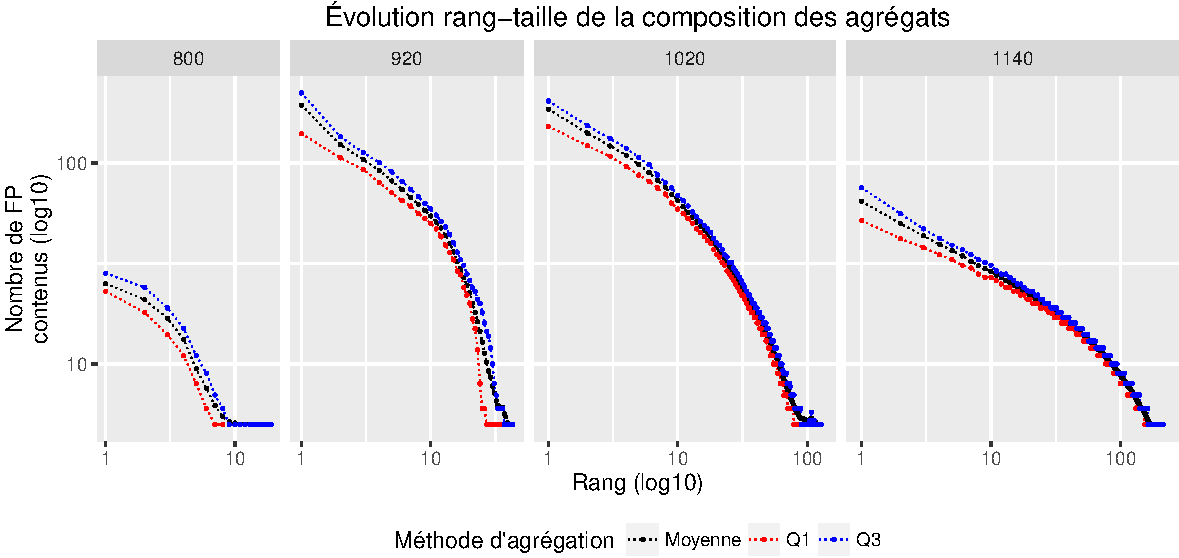
\includegraphics[width=.8\linewidth]{img/resultats/v0_rt_agregats.pdf}
	\caption{Évolution de la courbe rang-taille des agrégats.} 
	\label{fig:rt-agregats-v0} 
\end{figure}

\begin{figure}[H]
	\captionsetup{width=\linewidth}
	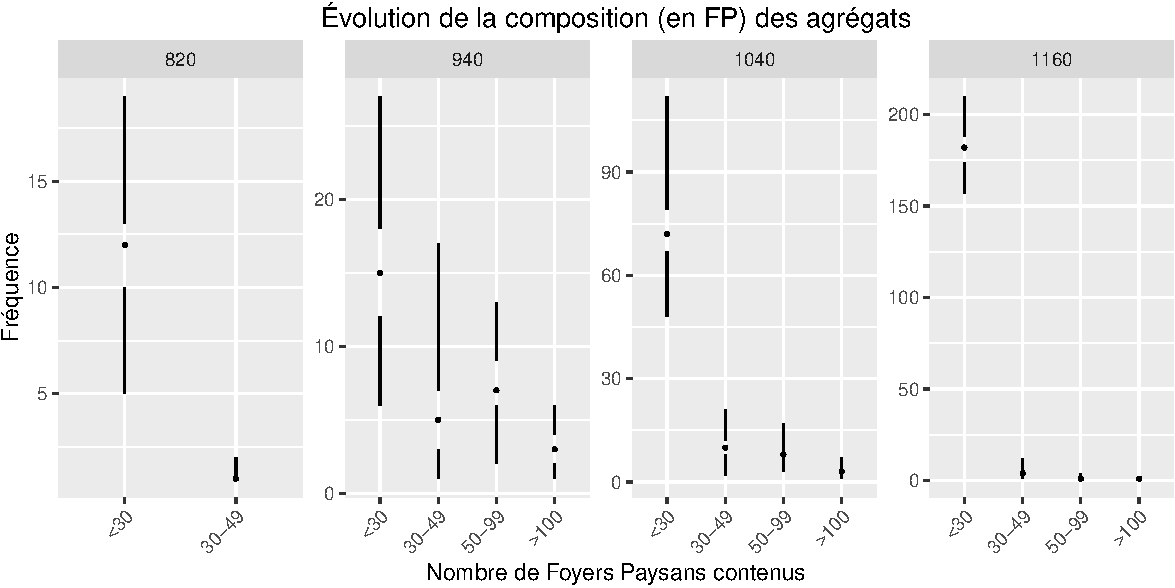
\includegraphics[width=.8\linewidth]{img/resultats/v0_compo_agregats.pdf}
	\caption{Évolution de la composition des agrégats.} 
	\label{fig:compo-agregats-v0} 
\end{figure}

\clearpage

\subsubsection{Hiérarchie des pôles}

La hiérarchie des agrégats donne une bonne vision agrégée de la hiérarchisation du système de peuplement dans son ensemble.
Pour autant, afin d'appréhender la dynamique de cette dimension, il est là encore nécessaire d'observer le comportement des composantes qui provoquent cette hiérarchisation.
En effet, une forte hiérarchie des pôles entraînera une attractivité des foyers paysans très inégale \footnote{En raison des logiques d'attachement préférentiel, voir la note de bas de page \ref{ftn:preferential-attachment} page \pageref{ftn:preferential-attachment}.} De plus, comme indiqué plus haut, on cherche à obtenir une forte hiérarchi)e pour les différents types d'agents du modèle.
L'observation de la hiérarchie des pôles est donc importante pour évaluer le modèle SimFeodal.
Pour déterminer cette hiérarchie, on peut se fier à deux indicateurs complémentaires :
le nombre d'attracteurs composant chaque pôle et l'attractivité de ces derniers.
Ces indicateurs de sortie sont proches, mais apportent pourtant une vision légèrement différente :
étant donné que chaque attracteur influe différemment, selon son type, sur l'attractivité globale d'un pôle, l'information sur l'attractivité et sur la composition ne sont pas redondantes, bien que fortement corrélées.
On aurait pu présenter une information plus détaillée quant à cette composition, par exemple en différenciant le nombre de chacun des types d'attracteurs de chaque pôle, mais le nombre de combinaisons possible aurait rendu cette information confuse.

À partir des connaissances expertes qui guident l'évaluation de SimFeodal, on cherche à obtenir, pour ces deux indicateurs, une courbe d'allure similaire, c'est-à-dire une courbe décroissante, avec bien plus de pôles mineurs (faible attractivité ou nombre d'attracteurs) que de pôles plus importants.
On cherche de plus à ce que cette courbe présente une allure log-normale, et donc que la proportion de pôles décroisse fortement à mesure que leur importance augmente.


\begin{mdframed}[backgroundcolor=gray!10,footnoteinside=false]
	Dans l'ensemble, on peut remarquer sur les deux indicateurs de la \cref{fig:compo-poles-v0} que les pôles, dans cette version 0, sont très hiérarchisés.
	La tendance \og évolutive va dans le bon sens :
	depuis une quasi-uniformité en 820, des pôles plus importants apparaissent et semblent se renforcer au cours du temps.
	On retrouve aussi, en observant les axes des ordonnées, la croissance du nombre de pôles identifiée plus haut (\ref{para:nb-poles}, \cnameref{para:nb-poles}, p. \pageref{para:nb-poles}) :
	de nouveaux pôles apparaissent tout au long de la simulation, et restent majoritairement peu importants, quand les pôles ayant commencé à se renforcer tôt continuent dans cette tendance.
	
	En fin de période, les pôles sont très hiérarchisés, aussi bien en matière de composition que d'attractivité.
	Ils le sont même plus que ce que les connaissances expertes laissent entendre :
	au delà de $0.66$ en attractivité ou de $4$ attracteurs, on ne dénombre plus qu'un unique pôle de chaque importance, là où on attendrait que cette courbe continue plutôt à décroitre.
	De plus, ces courbes montrent la variation des réplications de la version 0.
	Dès lors, on peut considérer que ces pôles majeurs ne sont en fait qu'un unique pôle (le plus souvent) d'importance variable selon les réplications, mais dans tous les cas d'importance bien supérieure aux pôles qui arrivent juste après dans le classement.
	Cette macrocéphalie ne correspond pas aux observations empiriques, d'autant que rappelons-le, la ville de Tours n'est pas modélisée dans SimFeodal.	
	
	
\end{mdframed}

\begin{figure}[H]
	\captionsetup{width=\linewidth}
	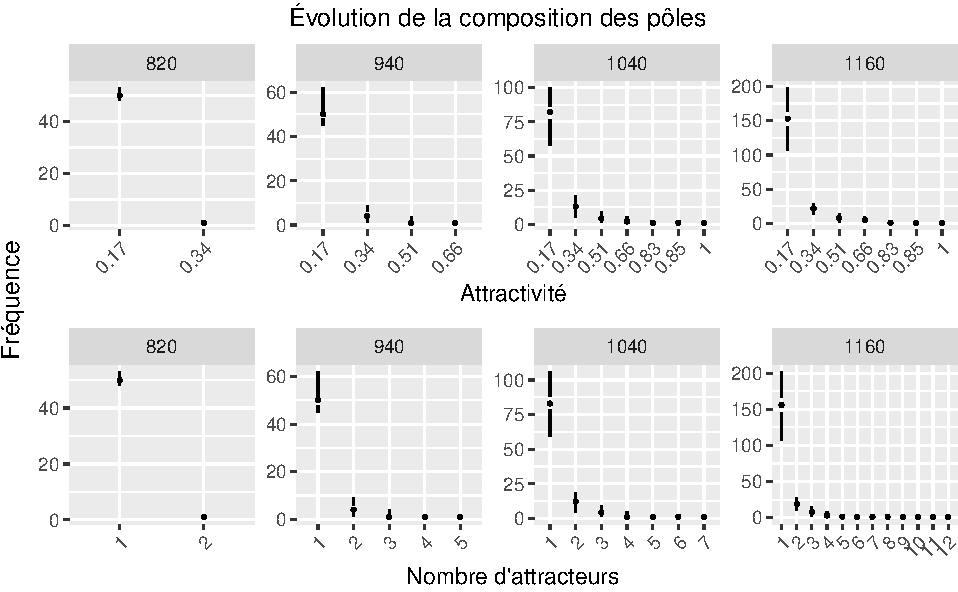
\includegraphics[width=\linewidth]{img/resultats/v0_compo_poles.pdf}
	\caption{Évolution de la composition et de l'attractivité des pôles\protect\footnotemark{}.} 
	\label{fig:compo-poles-v0}
\end{figure}
\footnotetext{\hl{Les figures ne sont pas en log-log (ou log-lin) et on ne voit donc pas vraiment le haut de la hiérarchie.
		Peut-être faudrait-il changer ces axes, mais ça complexifiera la lecture pour les archéos/lecteurs non habitués aux axes log}}

\clearpage

\subsubsection{Hiérarchie des paroisses}\label{par:hierarchie-paroisses}

A l'instar des pôles, on attend aussi des ressorts paroissiaux d'être hiérarchisés.
La période modélisée voit ainsi apparaître ces paroisses qui auront un rôle majeur dans la fixation du peuplement, et, pré-figurant le maillage communal, ont un double rôle de desserte efficace\footnote{C'est-à-dire desservir de manière optimale la plupart de la population.} et équitable\footnote{C'est-à-dire faire en sorte que même les populations les plus isolées aient un accès aussi rapide que possible à une église paroissiale.}.
En effet, avec la volonté d'encadrement et de prélèvement de l'Église sur la population, de nouvelles paroisses apparaissent pour desservir au mieux leurs potentielles ouailles.
Une structure double en résulte :
dans les zones les moins denses, le maillage est régulier mais lâche, de manière à minimiser le nombre d'églises paroissiales tout en s'assurant que chacun puisse y accéder dans un temps raisonnable\footnote{Cette distance-temps évolue au cours du temps, en fonction de l'accroissement de la fréquence de l'obligation de fréquentation des églises paroissiales.}.
Il y a donc un certain nombre d'églises paroissiales desservant peu de paroissiens.
Au contraire, dans les zones les plus denses, et en particulier au sein des petites villes naissantes, l'objectif est d'être au plus près des résidents tout en garantissant à chacun de pouvoir assister aux différents offices :
il y donc une croissance du nombre d'églises paroissiales proches les unes des autres, visant à accompagner un encadrement maximum de la population, ainsi, avec une logique concurrentielle de ce clergé féodal, qu'à capter l'importante source de revenus qu'assure la collecte de la dîme.
Cette logique concurrentielle doit aussi permettre de restreindre le nombre de foyers paysans desservis par une unique paroisse.

On s'attend donc à avoir une courbe hiérarchisée dans la lignée d'une courbe log-normale, mais avec toutefois un double seuil minimal (l'effet de \og longue traîne\fg{}), autour des paroisses \og rurales\fg{} peu peuplées (moins de 10 foyers paysans désservis) et des paroisses du bas de la hiérarchie classique, peuplées de 10 à 40 foyers paysans\footnote{D'après les valeurs des paramètres \texttt{nb\_min\_paroissiens} et \texttt{nb\_max\_paroissiens}}).

\todobox{ici, impérativement, il faudra mettre un graphique schématique de ce qu'on attend.}

\begin{mdframed}[backgroundcolor=gray!10,footnoteinside=false]
	En fin de simulation de cette version 0, la hiérarchie des paroisses est plutôt satisfaisante.
	On y retrouve en effet une forte hiérarchie, peut-être même légèrement trop importante.
	Il ne devrait ainsi par y avoir de paroisse composée de plus de $100$ foyers paysans en fin de simulation, et la courbe présente une pente trop importante (celles de 940 ou 1040 sont ainsi plus conformes aux attentes).
	Pour autant, on remarque bien un effet de hiérarchisation au cours du temps, ainsi qu'un accroissement du nombre de petites paroisses, montrant que la dynamique, bien que non ajustée, s'inscrit bien dans la dynamique observée empiriquement.
	(\cref{fig:compo-paroisses-v0})
\end{mdframed}

\begin{figure}[H]
	\captionsetup{width=\linewidth}
	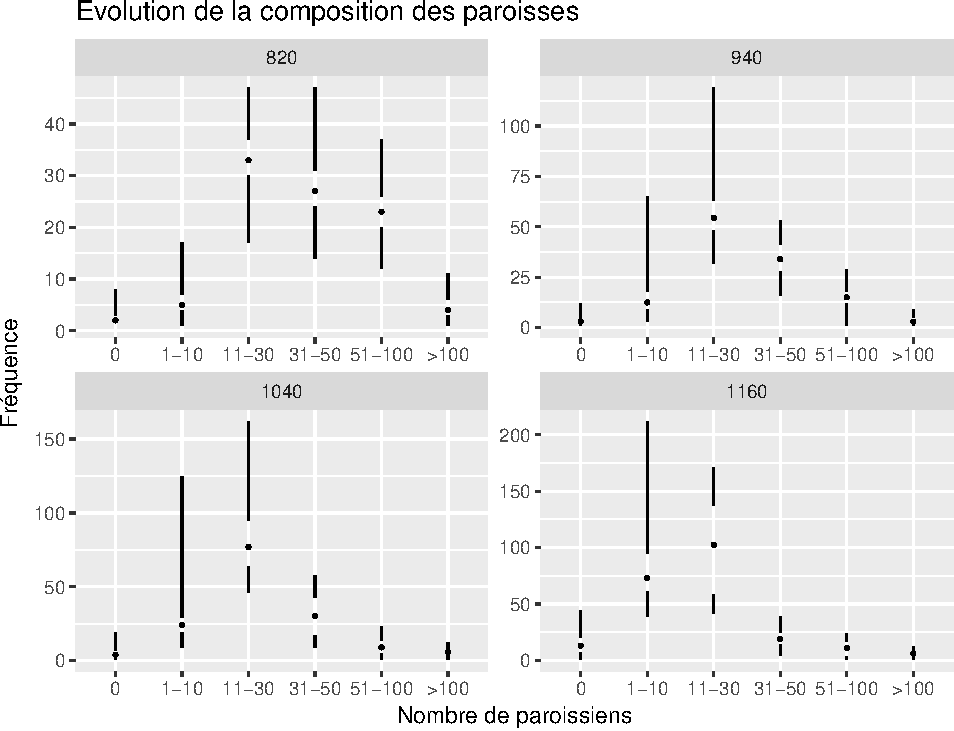
\includegraphics[width=\linewidth]{img/resultats/v0_compo_paroisses.pdf}
	\caption{Évolution de la composition des paroisses.} 
	\label{fig:compo-paroisses-v0} 
\end{figure}

\clearpage

\subsection{Évaluer la fixation et la dissémination du peuplement}


La dernière dimension étudiée par SimFeodal est moins définie que les précédentes.
On y observe ainsi la fixation du système de peuplement au sein du maillage naissant que constituent les paroisses.
Cette notion de fixation pose problème par rapport à l'ensemble des indicateurs de sortie déployés jusqu'ici.
En effet, SimFeodal est un modèle fondé sur un temps discret :
on y observe, à chaque itération, le résultat des processus modélisés.
On peut y observer une fixation d'un pas de temps par rapport à l'autre, par exemple en constatant qu'un agrégat constitué en 820 semble être toujours présent en 840.
On peut de plus considérer que cet agrégat présente les mêmes caractéristiques au deux dates, en matière de localisation et de population.
L'agrégat est donc stable dans le temps.
L'échelle d'analyse mobilisée dans les indicateurs précédents -- au niveau agrégé des agrégats, voir du système d'agrégats -- pourrait donc s'appliquer ici aussi.
Pourtant, quand on parle de fixation des foyers paysans, ce qui est observé empiriquement, il n'est pas question d'agrégats, mais des entités les composant, c'est-à-dire les foyers paysans.
Ceux-ci ne sont pas observés directement quand on remarque que les agrégats semblent stable :
on approche là à la différence entre un état stable et un état stationnaire.
La relative stationnarité des agrégats dans le temps n'est ainsi pas garante de stabilité de leurs composantes :
deux foyers paysans oscillant d'un agrégat à un autre, dans un mouvement opposé, produiraient ainsi une stationnarité de ces agrégats, mais, en se déplaçant, ils ne satisferaient pas au critère de fixation.
Il y a donc un problème de changement d'échelle pour observer la fixation des foyers paysans :
il n'est plus possible de raisonner à l'échelle des agrégats, et il faut se concentrer sur celle des foyers paysans.

Cette échelle pose un autre problème :
les foyers paysans sont très nombreux ($4000$ dans la version 0) et se déplacent.
Ils se déplacent de plus selon des modalités très différentes (\hl{Faire ref aux mécanismes de déplacement du chapitre 2}), rendant complexe la caractérisation des mouvements de chacun et plus encore celle d'une agrégation de ces catégories.

Pour ces raisons, la production d'indicateurs synthétiques spatiaux -- une ou plusieurs cartes -- ne suffirait pas à communiquer une information intelligible sur l'éventuelle fixation des foyers paysans.
Il nous faut donc faire appel à des \og proxys\fg{}, non spatiaux, pour évaluer la fixation des foyers paysans.

A cet effet, on a retenu des indicateurs relatifs aux déplacements des foyers paysans et à leur raison :
combien de foyers paysans se déplacent à chaque pas de temps (moins il y a de déplacement, plus la fixation est importante) ? Quelles sont les modalités de ces déplacements (un déplacement entre deux agrégats lointains n'a pas les mêmes conséquences en terme de stabilité qu'un déplacement minime au sein d'un même agrégat) ? Ou encore, comment évolue la satisfaction des foyers paysans, et avec celle-ci, la probabilité de se déplacer ?

Ces indicateurs permettent d'évaluer la capacité du modèle à reproduire la fixation des foyers paysans.
Pour autant, la contrainte est ici double :
on recherche une fixation, mais celle-ci est, empiriquement, supposée se dérouler et se voir renforcer par la mise en place du maillage paroissiale qui doit servir de support à la nouvelle configuration spatiale émergente.

On s'appuiera donc aussi sur des indicateurs relatifs à cet espace support constitué par les paroisses :
leur nombre, leur dispersion dans l'espace et l'efficacité de la desserte qu'elles assurent.

\paragraph*{}Notons que contrairement aux deux précédents dimensions d'analyse, nous n'établissons ici pas de hiérarchie nette entre les indicateurs.
Cette étude de la fixation est moins facilement appréhendable que celle de la polarisation ou de la hiérarchisation et les indicateurs qui la caractérisent apportent une complémentarité de points de vue plus qu'un affinement de l'évaluation de cette dynamique.
Dès lors, les indicateurs présentés ci-après ne peuvent être catégorisés en indicateurs principaux et secondaires.
On retrouvera cependant cette hiérarchie d'évaluation au sein des indicateurs, par exemple en suivant l'ordre des graphiques présentés.
Par exemple, pour évaluer la fixation des foyers paysans, on observera d'abord le résultat produit (nombre de déplacements) avant d'entrer dans le détail de sa composition (types des déplacements).


\subsubsection{Déplacement des foyers paysans}

Le déplacement des foyers paysans est l'élément moteur de SimFeodal :
c'est par le déplacement individuel de chacun des foyers paysans que la configuration spatiale évolue.
Les déplacements affectent donc chacune des dimensions d'analyse -- polarisation, hiérarchisation et fixation --, mais c'est au sein de cette dernière qu'il est le plus intéressant de les observer.
Il est en effet attendu que de nombreux déplacement surviennent, afin que le système de peuplement puisse se structurer, mais pour autant, il est aussi nécessaire que ces déplacements tendent à diminuer au cours du temps, une fois le système en voie de stabilisation.

On pourrait donc attendre que les déplacements suivent une courbe négative (linéaire ou non) tendant vers 0, impliquant une absence de déplacements en fin de période.
Pour autant, le mécanisme de déplacement est sans doute l'un des plus complexes du modèle, et on ne peut l'appréhender aussi simplement.

En premier lieu, les mécanismes de SimFeodal différencient deux types de déplacements (\hl{Faire ref à chap2}) :
les déplacements locaux (dans un rayon de $2500$m dans la version 0) et les déplacements lointains.

\begin{itemize}
	\item Les déplacements locaux visent à faire s'agréger des foyers paysans dispersés autour de pôles présents à proximités.
	Ce mécanisme peut être présent sur toute la durée de la simulation, sur un effectif faible.
	En effet, cet effet d'agrégation locale permet \og d'optimiser\fg{} la répartition spatiale des agrégats, en renforçant leur hiérarchie et en faisant fusionner des agrégats qui seraient très proches les uns des autres.
	Pour autant, dans un objectif de fixation du peuplement, il est nécessaire de veiller à ce que les foyers paysans ne soient pas amenés à se déplacer localement de manière continuelle, par exemple en faisant des allers-retours entre des pôles ou agrégats spatialement proches.
	
	\item Les déplacements lointains servent un autre rôle :
	un foyer paysan qui ne serait pas en mesure d'augmenter sa satisfaction localement -- faute de pôles suffisamment attractifs dans le voisinage -- a une probabilité de se déplacer vers un agrégat situé n'importe où dans l'espace modélisé.
	Le modèle est très sensible à ce mécanisme qui agit comme une perturbation forte dans la structure spatiale du peuplement.
	Ce mécanisme \og de dernier recours\fg{} ne doit être employé que rarement, en cas de situations où des foyers paysans seraient trop isolés pour pouvoir s'agréger localement.
	C'est notamment le cas pour les foyers paysans nouveaux arrivants, via le mécanisme de renouvellement (\hl{ref dans chap 2}), qui peuvent se voir localisés n'importe où dans l'espace du modèle.
\end{itemize}

Pour ajouter à la complexité du mécanisme, et donc de l'évaluation de cet indicateur qu'est le nombre de déplacements au cours du temps, rappelons que différentes contraintes temporelles viennent bouleverser, à dessein, le comportement des foyers paysans.
En particulier, entre 950 et 1050, les modalités d'évaluation de la satisfaction deviennent plus strictes (\hl{Voir dans chap2, frise}).
Cela engendre nécessairement une plus forte propension des foyers à se déplacer.

Si les connaissances empiriques d'un tel niveau de finesse ne sont pas disponibles, on peut tout de même avoir des attentes quant au comportement attendu du modèle.
Au regard des éléments décrits plus haut, on peut ainsi chercher à ce que l'évolution des déplacements suive plusieurs rythmes au cours du temps :
\begin{enumerate}
	\item Dans une première phase, du début de la simulation jusqu'aux perturbations débutant en 950 :
	quelques déplacements lointains marginaux ($\approx 5$\% à $10$\%), stables au cours du temps ; et de plus nombreux (au moins $\approx 30$\%) déplacements locaux menant à la constitution de petits agrégats locaux.
	Les déplacements locaux doivent diminuer au cours du temps, une fois les agrégats constitués.
	\item Pendant la deuxième phase, entre 950 et 1050, les nombreuses perturbations devraient voir une nette augmentation des déplacements locaux, et dans une moindre mesure lointains, prémices à la constitution d'agrégats plus hiérarchisés.
	\item Après ces perturbations, on devrait retrouver le niveau de déplacement de la seconde période, et là aussi, tendre vers une diminution des déplacements locaux, le système se stabilisant à l'approche de la fin de la période.
\end{enumerate}

Tout au long de cette période, on cherche de plus à ce que les foyers paysans soient polarisés, c'est-à-dire ici, qu'ils se regroupent dans des agrégats de population.
Parmi les modalités de déplacement, un autre indicateur utile est ainsi l'observation des provenances et destinations des foyers paysans qui se déplacent :
plus les foyers paysans originellement dispersés auront tendance à rejoindre des agrégats, plus la simulation sera satisfaisante au regard des hypothèses empiriquement émises.


\begin{mdframed}[backgroundcolor=gray!10,footnoteinside=false]
	Dans cette version 0 de SimFeodal, il apparaît en premier lieu que les déplacements sont trop peu nombreux (\cref{fig:nb-deplacements-v0}).
	Les déplacements lointains sont à peu près dans les proportions attendues, mais les déplacements locaux sont trop peu nombreux.
	Surtout, les trois phases attendues ne se retrouvent pas sur ces sorties.
	On y remarque bien l'impact des perturbations, mais celles-ci ne font qu'augmenter la part de déplacements, laquelle reste stable avant et après ces perturbations.
	La version 0 de SimFeodal n'est donc pas satisfaisante en termes de stabilisation et de fixation des foyers paysans.
	L'observation des modalités de déplacement (\cref{fig:type-deplacements-v0}) montre certes une part croissante de déplacements \og Isolé -> Agrégé\fg{}, mais dans des proportions là aussi trop faibles passé le tout début de la simulation.
\end{mdframed}

\begin{figure}[H]
	\captionsetup{width=\linewidth}
	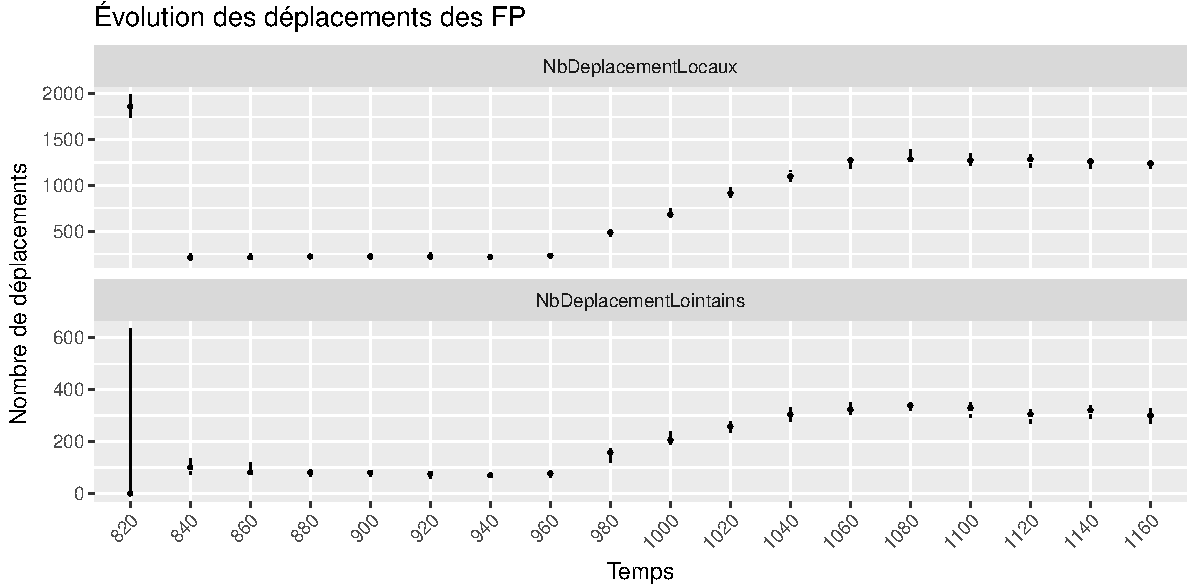
\includegraphics[width=\linewidth]{img/resultats/v0_nombre_deplacements.pdf}
	\caption{Évolution du nombre de déplacement des foyers paysans.\\
		\todobox{Mettre le graphique en relatif}} 
	\label{fig:nb-deplacements-v0} 
\end{figure}



\begin{figure}[H]
	\captionsetup{width=\linewidth}
	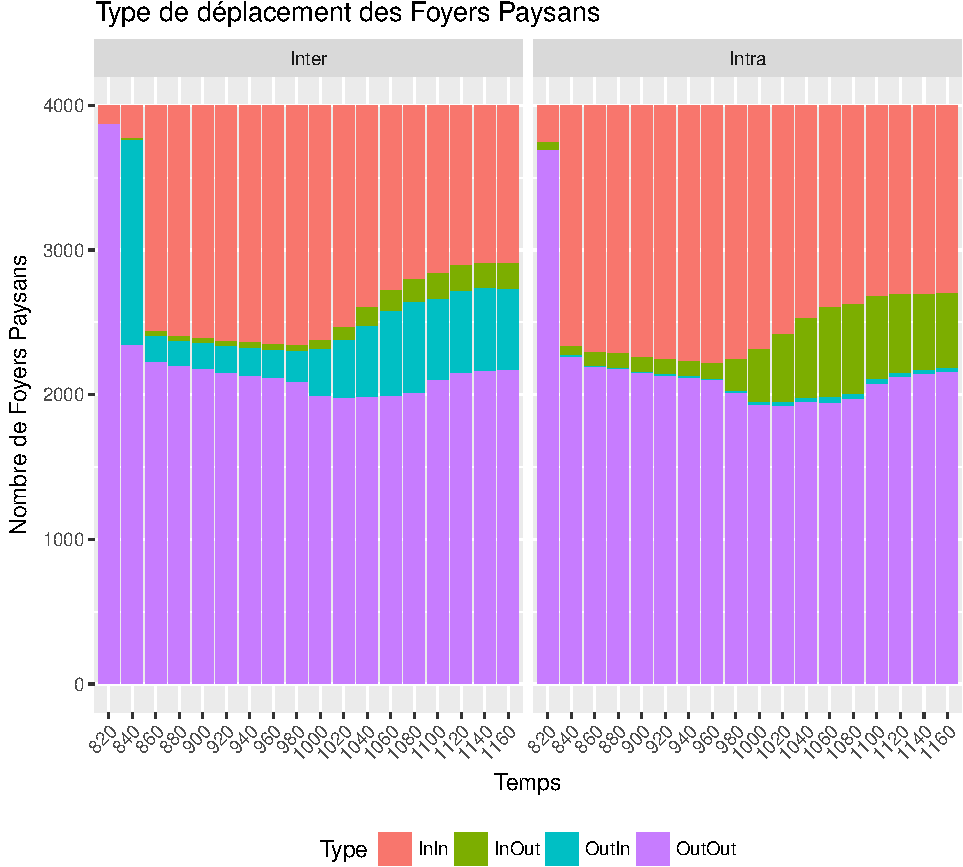
\includegraphics[width=\linewidth]{img/resultats/v0_types_deplacements.pdf}
	\caption{Évolution des types de déplacement des foyers paysans.\\
		Inter : Déplacement depuis le pas de temps précédent vs Intra :
		déplacement au sein d'un même pas de temps.
		\todobox{Ne garder que l'inter et mettre le graphique en relatif}\\
		%	- InIn : Le FP était dans un agrégat au pas de temps précédent, et est dans un agrégat à ce tour (quel qu'il  soit, ça peut être le même ou un autre).\\
		%	- InOut : Le FP était dans un agrégat au pas de temps précédent, et est isolé à ce tour\\
		%	- OutIn : Le FP était isolé, et est maintenant dans un agrégat\\
		%	- OutOut : Le FP était isolé, et l'est toujours\\
		%On constate donc que les déplacements au sein d'un tour tendent à isoler les FP, grosso modo dans le même temps et les mêmes proportions que la stabilisation du taux de FP isolés.	
	} 
	\label{fig:type-deplacements-v0} 
\end{figure}

\clearpage

\subsubsection{Satisfaction des foyers paysans}

On a vu dans les deux indicateurs précédents que les déplacements des foyers paysans sont très affectés par leur niveau de satisfaction.
Pour comprendre ces déplacements, il est donc utile d'observer en détail l'évolution de la satisfaction qui les provoquent.

La satisfaction ne saurait être résumée en un simple indicateur de fixation, tant son rôle est prépondérant dans une large partie des mécanismes du modèle.
Pourtant, mobilisé ici, cet indicateur apporte un éclairage différent.
Il permet ainsi de préciser les indicateurs précédents en donnant une explication à leur éventuelle mauvaise réponse aux attentes.

Ainsi, une satisfaction globalement trop élevée ne serait pas assez motrice à des déplacements, résultant en une polarisation faible.
Au contraire, une satisfaction globalement faible engendrerait une très forte mobilité, par exemple sous forme de mouvements pendulaires, d'où une absence de fixation du peuplement.
Comme pour les déplacements, on attend, depuis les connaissances empiriques, qu'il y ait trois phases dans l'évolution de cette satisfaction :
(1) une première phase, jusqu'en 950, où les foyers paysans sont globalement satisfaits, et le sont de plus en plus à mesure qu'ils s'agrègent ;
(2) une seconde phase, entre 950 et 1050, où les restrictions fortes (distance à un château, à une église paroissiale) auront pour effet de violemment abaisser le niveau de satisfaction ;
et enfin, (3) une dernière phase où, passées les perturbations, le niveau de satisfaction tend à remonter doucement, sous l'effet de l'agrégation et de la constitution généralisées de communautés paysannes et de la construction de châteaux et de nouvelles églises paroissiales.

\begin{mdframed}[backgroundcolor=gray!10,footnoteinside=false]
	Au vu des résultats de la version 0 de SimFeodal illsutrés dans la \cref{fig:satisfaction-fp-v0}, on constate que les trois phases attendues sont bien présentes.
	La perturbation en milieu de période est très forte, mais pourtant, le niveau de satisfaction général reste très élevé (à toute date, plus de $80$\% des foyers paysans ont une satisfaction supérieure à $0.5$).
	Avec ce niveau de satisfaction et les mécanismes de déplacement de cette version 0, seuls les foyers paysans à proximité de très gros pôles (au moins un gros château et plusieurs églises paroissiales) pourront se déplacer localement.
	Et pour peu qu'il y ait plusieurs pôles importants à proximité, ils oscilleront entre les deux, gonflant artificiellement le nombre de déplacements locaux.
	L'observation de cet indicateur confirme que le niveau de déplacement est trop faible et ne présente pas l'allure attendue, tout en donnant une explication à la mauvaise fixation du peuplement observée.
\end{mdframed}

\begin{figure}[H]
	\captionsetup{width=\linewidth}
	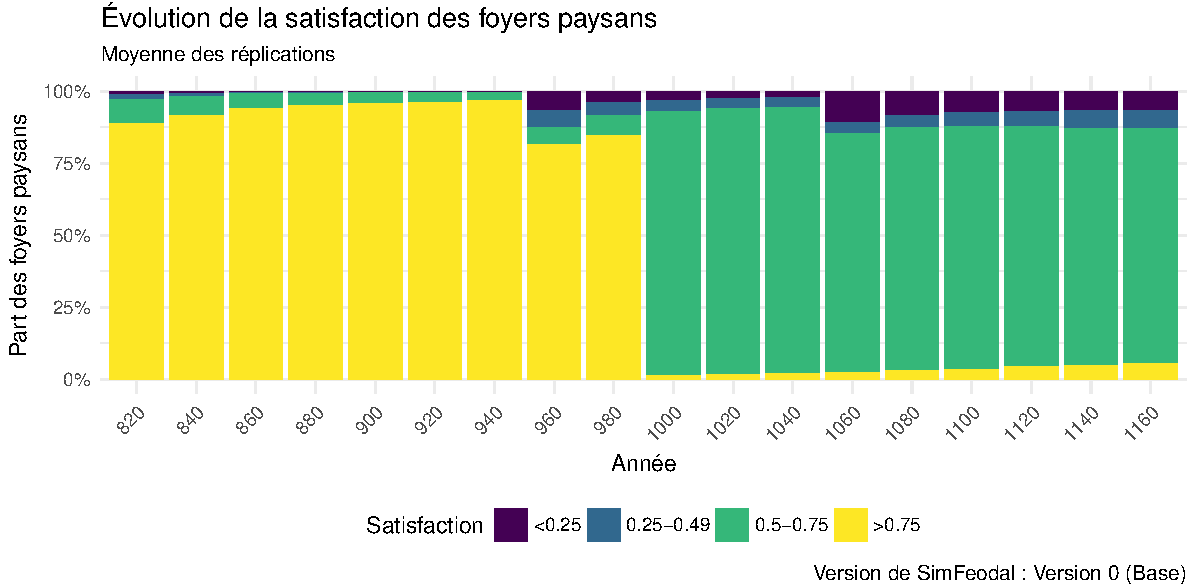
\includegraphics[width=0.95\linewidth]{img/resultats/v0_satisfaction_fp.pdf}
	\caption{Satisfaction des foyers paysans} 
	\label{fig:satisfaction-fp-v0} 
\end{figure}

\clearpage

\subsubsection{Nombre et dispersion des paroisses}

Tout au long de la période, de nouvelles églises paroissiales sont créées (\hl{cf. mécanisme dans chap. 2}) et viennent renforcer l'encadrement des foyers paysans.
L'évolution du maillage constitué par les ressorts paroissiaux représente donc l'évolution de la structure spatiale des foyers paysans.
Pour que les foyers paysans soient satisfaits, il faut, à partir de 950, qu'ils soient suffisament proches d'une église paroissiale
Celles-ci constituent donc, à mesure de l'avancement de la période, des pôles qui vont aider à la fixation des foyers paysans.
Il est donc légitime d'observer la croissance du nombre et la répartition des paroisses telles que simulées dans le modèle SimFeodal.

Sur un plan purement numéraire, plus les paroisses seront nombreuses, mieux la population sera desservie, et moins les foyers paysans se déplaceront : la fixation sera donc plus forte à mesure que le nombre de paroisses augmente.
Sur un plan spatial, l'accumulation de paroisses en zones denses (dans des agrégats de populations) doit renforcer la polarisation de ces zones, et avec elle, accroître les chances de fixation des foyers paysans.

D'après les mécanismes mis en places dans cette version 0 de SimFeodal, on s'attend donc à ce que le nombre de paroisses augmente régulièrement au cours du temps, depuis un nombre initial évalué à $50$ en $800$, jusqu'à atteindre un objectif numérique fixé à $200$ d'après les connaissances empiriques de la région modélisée.

Concernant la répartition spatiale, on cherche à atteindre le double phénomène décrit dans la partie \ref{par:hierarchie-paroisses} (\cnameref{par:hierarchie-paroisses}, p. \pageref{par:hierarchie-paroisses}).
Spatialement, cela devrait mener à une diminution de la superficie des paroisses les plus larges dans les zones peu denses.
Dans les zones plus denses, concentrant les agrégats, cela devrait aussi mener à une diminution de la superficie, bien plus drastique cependant : avec la création de nouvelles paroisses au sein des agrégats, on devrait voir apparaître de nombreuses paroisses se partageant un espace très réduit.

Notons que la dispersion des agrégats et des pôles, vue précédemment (\ref{par:polarisation-dispersion}, \cnameref{par:polarisation-dispersion}, p. \pageref{par:polarisation-dispersion}), constituerait ici aussi un bon indicateur de fixation, en observant non plus l'évolution de la couverture spatiale, mais plutôt la fixation et le renforcement des dynamiques locales de polarisation.

\begin{mdframed}[backgroundcolor=gray!10,footnoteinside=false]
	Dans la version 0 de SimFeodal, on peut en premier lieu constater que la tendance -- à la croissance -- de l'évolution du nombre de paroisses est bonne (\cref{fig:nb-paroisses-v0}).
	Ainsi, de nouvelles églises paroissiales sont bien créées ou promues régulièrement au cours du temps.
	La quantité atteinte ($240$ en moyenne) dépasse un peu trop fortement l'objectif empirique, mais surtout, on remarque dans la figure la très forte variabilité de ces résultats (l'intervalle interquartile est de 100). De plus, cette variabilité augmente fortement avec le temps.
	
	La dynamique est donc plutôt satisfaisante, mais le nombre atteint autant que la variabilité sont améliorables et rendent clairement visible la nécessité d'un ajustement dans le modèle.
	
	Sur le plan spatial, la \cref{fig:densite-paroisses-v0} laisse bien apparaître la double évolution attendue : les paroisses les plus étendues, en périphérie, demeurent parmi les plus grandes mais voient leur superficie réduite à mesure que de nouvelles églises paroissiales y apparaissent.
	Dans le même temps, on remarque aussi les effets de fractionnement et de subdivision des paroisses les moins étendues.
	Cela résulte, dans la figure, en de nombreuses concentrations locales de paroisses que l'échelle des cartes nous permet plus de percevoir que de détailler précisément\footnotemark{}.
\end{mdframed}
\footnotetext{La trop forte hétérogénéité dans les superficies des paroisses rend difficile la lecture de l'espace.On pourrait y remédier par exemple avec des cartogrammes, mais alors, on ne verrait plus que ces zones de forte densité.}

\todobox{Là aussi, courbe et nombre du nombre de paroisses est incohérent entre chapitre TMD (154) et résultats JIAP (240), + variabilité très forte dans JIAP et pas dans TMD.}

\begin{figure}[H]
	\captionsetup{width=\linewidth}
	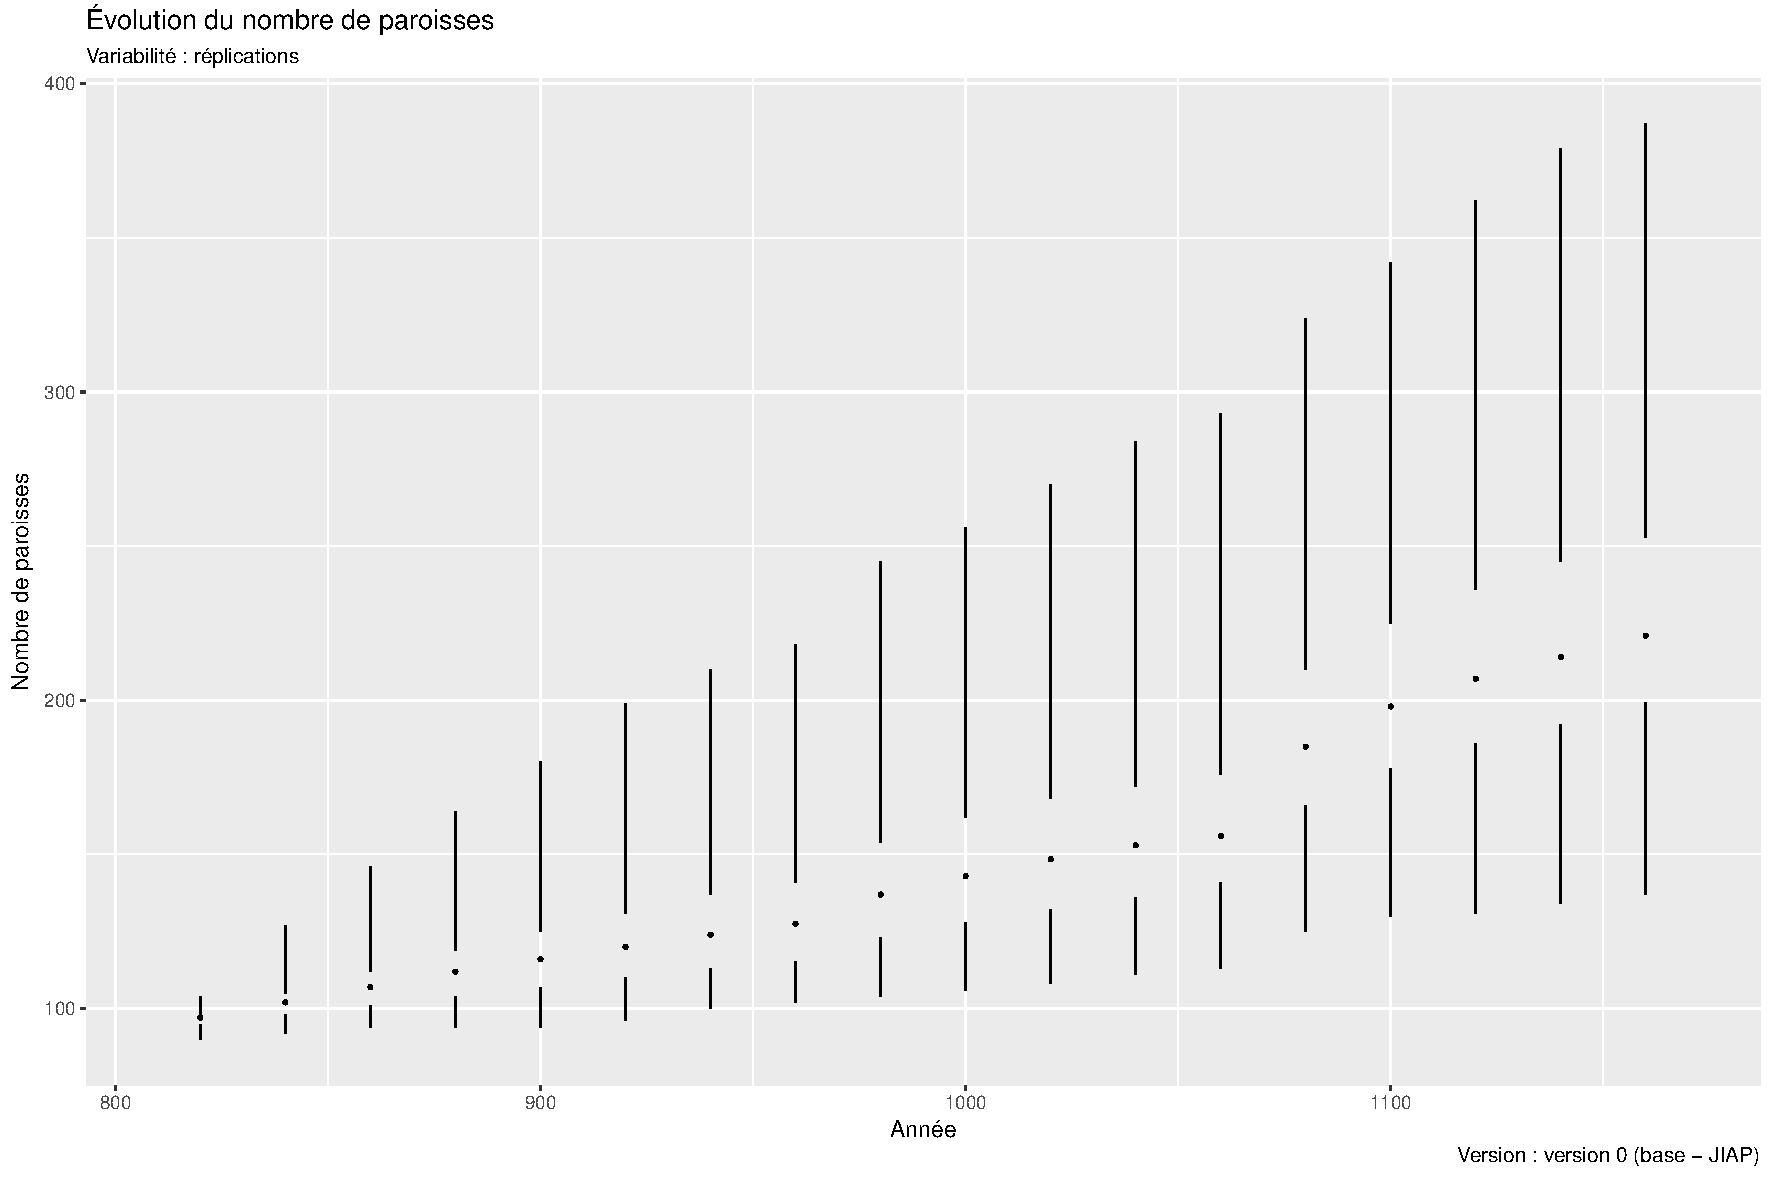
\includegraphics[width=0.75\linewidth]{img/resultats/v0_nombre_paroisses.pdf}
	\caption{Évolution du nombre de paroisses} 
	\label{fig:nb-paroisses-v0} 
\end{figure}

\begin{figure}[H]
	\captionsetup{width=\linewidth}
	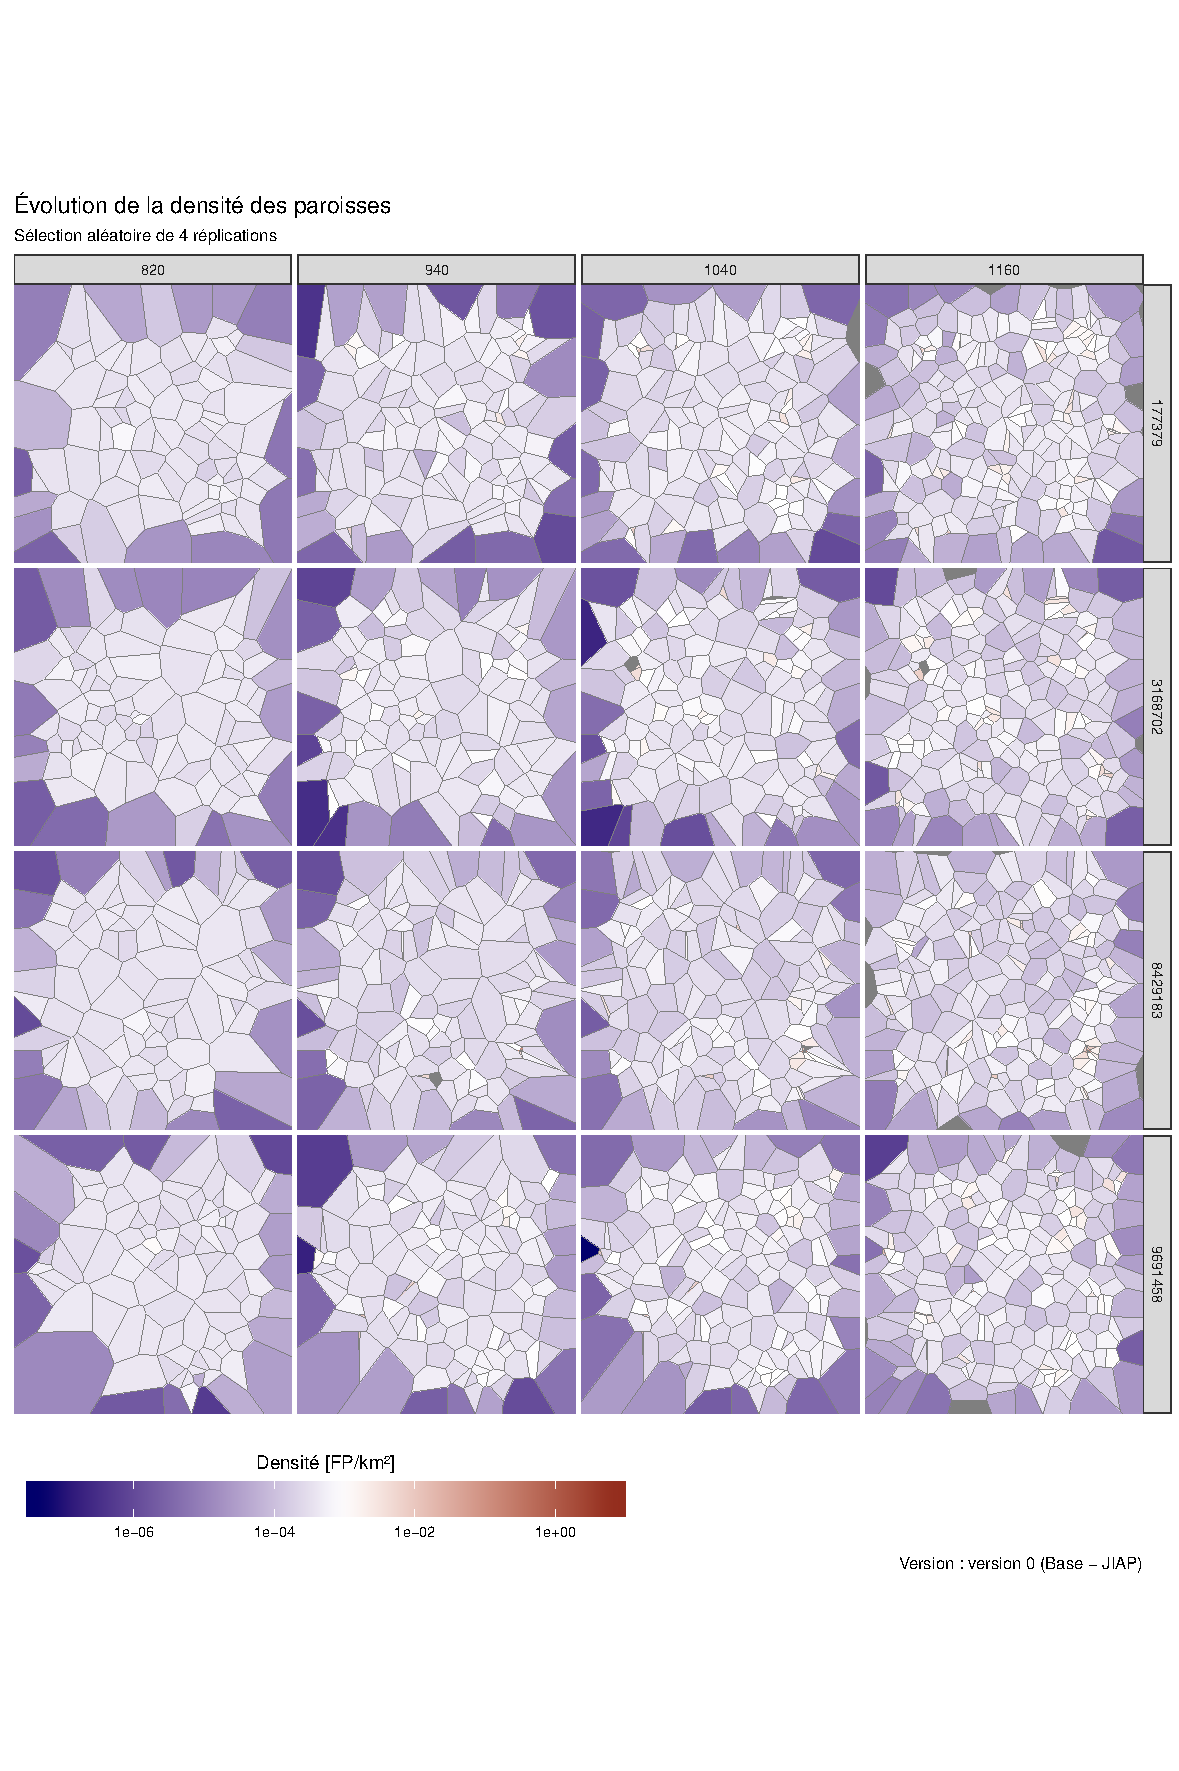
\includegraphics[width=0.8\linewidth]{img/resultats/v0_paroisses_densite.pdf}
	\caption{Densité des paroisses} 
	\label{fig:densite-paroisses-v0} 
\end{figure}


\clearpage

\subsubsection{Efficacité et équité de la desserte paroissiale}

On a vu précédemment (\ref{par:hierarchie-paroisses} , \cnameref{par:hierarchie-paroisses}, p. \pageref{par:hierarchie-paroisses}) que les paroisses devaient assurer conjointement une desserte efficace et équitable.
Un indicateur possible pour évaluer l'efficacité du maillage simulé est d'en observer la couverture spatiale.
Par définition, les paroisses couvrent ainsi l'ensemble du territoire simulé. 
Pour autant, certaines paroisses peuvent être très étendues, comme vu dans l'indicateur précédent.
On peut toutefois quantifier la dispersion de ces paroisses en analysant leur répartition spatiale, ou plutôt, celle des églises paroissiales qui en constituent le cœur.
Pour cela, on peut faire appel à une méthode d'analyse spatiale assez classique, similaire à la méthode des quadrats, en découpant l'espace en un maillage orthogonal régulier et en comptant le nombre d'églises paroissiales de chacune des mailles.
On a vu que dans SimFeodal, les églises paroissiales sont réparties de manière à la fois dispersée (zones de faible densité) et concentrées (zones denses à proximité des agrégats importants).
Plutôt que de faire un décompte des églises paroissiales et d'en tirer une hiérarchie, un indicateur plus simple est alors de faire un compte des mailles ne contenant pas de paroisse. Ces mailles étant régulières, l'indicateur résultant permettra alors d'appréhender simplement la part de l'espace couvert par des églises paroissiales.
On a choisi ici de discrétiser l'espace modélisé (de dimensions $100\times100$ km) en mailles de $10\times10$ km, pour un total de $100$ mailles de $100$km².
Ces valeurs permettent d'approcher, à grands traits, la configuration théorique qui verrait chacune des 300 églises paroissiales être réparties dans une maille différente\footnote{Il faudrait alors 300 mailles de $\approx$ 6 km de largeur, mais cette valeur ne constitue pas un multiple de 100. De plus, les églises paroissiales étant générées en partie au sein d'agrégats existants pour renforcer la desserte du plus grand nombre, cette valeur est très loin d'être accessible.}.

Selon les mécanismes de SimFeodal, on s'attend à ce que l'indicateur ainsi produit diminue au cours du temps, à mesure que de nouvelles églises paroissiales viennent desservir le territoire, de manière régulière (comme l'évolution du nombre d'églises paroissiales).
Cette diminution devrait toutefois être moins rapide que celle du nombre de paroisses, puisque les églises paroissiales créées au sein des agrégats devraient logiquement ne pas desservir de nouvelles mailles, mais plutôt se situer dans des mailles déjà occupées.

Du point de vue de l'équité de la desserte, on peut recourir à un indicateur plus partiel : il s'agit ici de décrire non pas l'évolution de la desserte des paroisses pour la plupart des foyers paysans, mais plutôt pour ceux d'entre eux qui seraient le plus isolés.
Ainsi, on peut observer l'évolution de la proximité entre les foyers paysans et les églises paroissiales, et ce, pour les paysans les plus éloignés desdites églises paroissiales à chaque pas de temps.
Une augmentation de l'équité devrait ainsi, par exemple pour les 10\% de foyers paysans les moins bien desservis, montrer une diminution de la distance moyenne aux églises paroissiales.

On s'attend ici aussi à voir une augmentation de l'équité, et donc une diminution au cours du temps de cette distance.
Empiriquement, on estime à $5$km la distance maximale à laquelle un foyer paysan se situait d'une église paroissiale en fin de période (\hl{Voir les seuils de distance dans chapitre 2}).
Un paramétrage de SimFeodal sera donc considérée comme satisfaisant, sur ce plan de l'équité de desserte, s'il voit cette distance converger vers le seuil, voire passer en dessous, de $5$km.


\todobox{Il manque un indicateur d'équité. A compléter une fois qu'il sera mis en place. Par exemple :\\
	Évolution de la distance des 10\% de FP les plus éloignés d'une/à une église paroissiale ? ==> Sans doute très intéressant, mais pas \og productible\fg{} pour l'instant. De toute façon, à voir les résultats JIAP, il faudra sans doute faire retourner toutes les itérations du modèle avec des sorties semblables à celles de la v8 (4\_4\_A)\\
	==> Peut être sous forme de boxplot ou d'histogramme (ridgeplot) ou de moyenne (plus influencée par grandes distances que médiane, donc mieux ici)}

\begin{mdframed}[backgroundcolor=gray!10,footnoteinside=false]
	
	En matière d'efficacité, la version 0 de SimFeodal est assez peu satisfaisante : malgré un nombre d'églises paroissiales trop élevé (voir l'indicateur précédent), la couverture du territoire est assez faible.
	En effet, la \cref{fig:couverture-paroisses-v0} montre qu'en fin de simulation, près de $90$\% de mailles restent inoccupées par des églises paroissiales.
	La tendance est toutefois à la diminution de ces mailles vides, et cette diminution est assez stable et régulière dans le temps.
	
	Comme dans le cas de l'évolution du nombre de paroisses, la variabilité est ici préoccupante et très insatisfaisante : l'écart interquartile est modéré (environ $15$\%), mais les minimums et maximums présentent un écart énorme (de $95$\% à $55$\%).
	
	\todobox{Pas possible d'analyser les résultats de la version 0 en matière d'équité sans les mesures correspondant. A faire une fois que les graphiques auront été produits.}
	
\end{mdframed}

\begin{figure}[H]
	\captionsetup{width=\linewidth}
	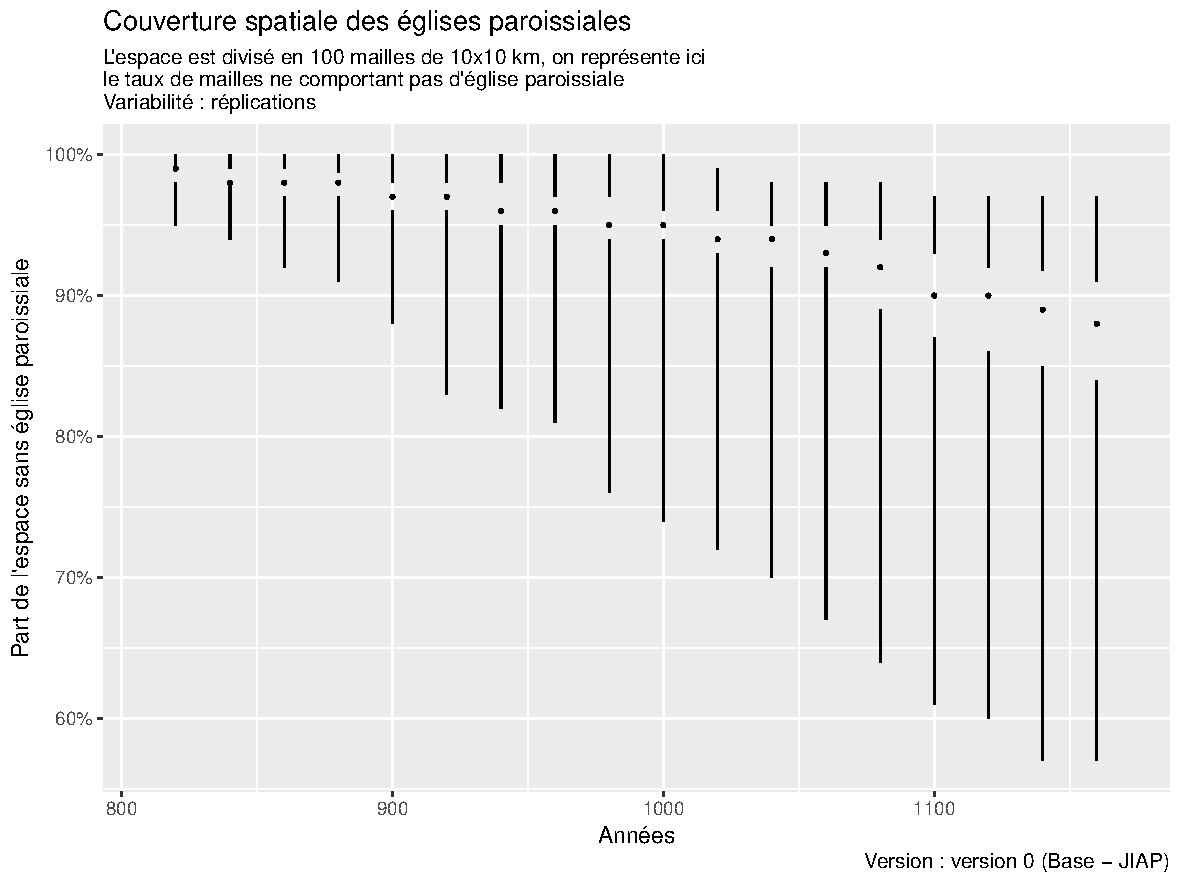
\includegraphics[width=0.9\linewidth]{img/resultats/v0_paroisses_occupation.pdf}
	\caption{Évolution de la couverture du territoire par les églises paroissiales.\\
		\todobox{Attention, résultats JIAP = pas fiables}
	} 
	\label{fig:couverture-paroisses-v0} 
\end{figure}
	
\end{document}

%
%\graphicspath{{chap4/}}
%\setcounter{chapter}{3}
%% !TEX root = ../These_TOC.tex
\chapter{Paramétrer un modèle dans un contexte de co-construction interdisciplinaire}
\label{chap:chap4}
\begin{center}
	{\large Version 2018-04-30}
\end{center}
\minitoc

Le modèle, tel qu'il a été présenté dans le chapitre précédent, était un \og état\fg{}, c'est-à-dire que les mécanismes, paramètres et les valeurs de ceux-ci correspondent à une étape d'un modèle amené à évoluer pour répondre aux problèmes soulevés dans la dernière partie (\hl{Ref dernière section chap 2}).
Dans ce chapitre, nous nous attacherons à présenter le travail de paramétrage réalisé à la suite, ayant abouti à une version plus adaptée aux questions des thématiciens. Le descriptif technique de cette version \og finale\fg{} se trouve dans l'annexe $n$ (\hl{Ref à l'annexe contenant le descriptif technique de la dernière version du modèle.})
Par paramétrage, nous entendons ici le processus visant à doter le modèle de paramètres (empiriques, \og commensurables\fg{} et techniques (\cref{enc:types-parametres})) lui permettant de mieux répondre aux objectifs fixé en termes de comportements attendus ou d'objectifs quantitatifs. Nous nous attacherons dans un premier temps à expliciter et spécifier ce sens.


% !TeX encoding = UTF-8
\clearpage
\section{Paramétrer ? Quoi et comment ?}

Avant de préciser le sens du terme \og paramétrage\fg{}, il semble important de définir précisément ce qu'est un paramètre. C'est en particulier nécessaire en ce que ce terme recouvre de nombreux sens selon les champs disciplinaires qui l'emploient, mais aussi, au sein même de ceux-ci, par les différents chercheurs.

\subsection{Différents points de vue sur la définition d'un paramètre}

Au plus général, le nouveau petit Robert définit un paramètre en ces mots :
\begin{quote}
	\og 1. \textsc{math.} Quantité à fixer librement, maintenue constante, dont dépend une fonction de variables indépendantes, une équation ou une expression mathématique. --- Variable en fonction de laquelle on exprime chacune des variables d'une équation.\\
	2. \textsc{fig.} et \textsc{didact.} Élément important dont la connaissance explicite les caractéristiques essentielles de l'ensemble d'une question.\\
	3. \textsc{par ext.} Élément nécessaire pour juger, évaluer, comprendre (qqch.).\fg{}\\
	\mbox{}~ \hfill \autocite[\textbf{Paramètre}]{robert_nouveau_1993}
\end{quote}


Seule la première définition correspond, à grands traits, à ce que l'on attend ici, mais elle est très généraliste, bien que ne correspondant pas pour autant à tous les usages du terme employés dans la littérature.

\subsubsection{En mathématiques, une définition univoque}
L'acceptation mathématiques d'un paramètre est sans doute celle qui souffre le moins d'ambiguïté : il s'agit des termes fixes d'une équation simple, par opposition aux variables qui en constituent les éléments qui seront amenés à évoluer.
Par exemple, dans la formulation d'une fonction affine, $f(x) = ax + b$, la valeur de $f(x)$ dépend de la variable $x$ et des paramètres fixés $a$ et $b$.
Quelles que soient les valeurs empruntées par $x$, ces paramètres demeurent constants. Dans une famille d'équations plus complexes, par exemple le modèle de croissance logistique de population\footnote{
	$\frac{\text{d}y}{\text{d}t} = \alpha y \times (1 - \frac{y}{K})$ d'après \autocite{verhulst1838notice}
}, l'accroissement de population au cours du temps ($\frac{\text{d}y}{\text{d}t}$) dépend de la valeur de la variable $y$, population à cet instant, ainsi que de deux paramètres, $\alpha$, le taux de croissance, et $K$, la \og capacité d'accueil\fg{}, c'est-à-dire un potentiel maximum de population vers laquelle tend -- et ne peut donc dépasser -- le système modélisé.
La définition mathématique est donc assez universelle et convient à la quasi-totalité des systèmes d'équations\footnote{A l'exclusion notable des systèmes d'équation paramétriques, où, à l'inverse, le terme de paramètre désigne alors les variables indépendantes.}.
Il convient toutefois de noter que la différence entre variable et paramètre est une affaire de point de vue, une inversion de perspective menant à échanger les paramètres et variables, tel que décrit dans l'exemple suivant :
\begin{quote}
	\og For the function $f(x)=ax^2+bx+c$, could we learn something by leaving the expression in terms of the symbols $a$, $b$, and $c$ and seeing how $f(x)$ depends on the parameters? Maybe we could fix $x=2$ and look how $f(2)$ changes as we let $a$ vary.
	
	If we do such manipulations and look at how the output of a function depends on varying a parameter, then we are treating the function as though the parameter were a input variable. But that's OK, as the difference between variables and parameters is really just a matter of perspective.\fg{}\\
	\mbox{}~ \hfill \autocite{nykamp_function_2015}
\end{quote}
On peut donc en retenir qu'en mathématiques, ce qui différencie la variable du paramètre est l'aspect fixe de ce dernier, au moins pendant la durée d'exécution d'une fonction : 
\begin{quote}
	\og{}A parameter is a quantity that influences the output or behavior of a mathematical object but is viewed as being held constant. [\dots]
	Variables are viewed as changing while parameters typically either don't change or change more slowly.\fg{}\\
	\mbox{}~ \hfill \autocite{nykamp_parameter_2015}
\end{quote}

% Conserver pour experiences etc. \footnote{
%		\og{}In some contexts, one can imagine performing multiple experiments, where the variables are changing through each experiment, but the parameters are held fixed during each experiment and only change between experiments.\fg{}\autocite{nykamp_parameter_2015}

On propose donc une une définition sans doute plus spécifique que celle du nouveau petit Robert, mais aussi plus tournée vers l'usage : un paramètre est une variable maintenue constante durant l'ensemble de l'utilisation d'une fonction.

\subsubsection{Une vision duale en statistiques}
En statistiques, quand bien même cette discipline fait un large usage des formalismes mathématiques, les paramètres recouvrent un ensemble assez différent : il s'agit d'une \og grandeur mesurable qui permet de présenter de façon plus simple, plus abrégée les caractéristiques essentielles d'un ensemble statistique.\fg{} \autocite[Paramètre, \textsc{stat.} (calcul des probabilités)]{tresor1992}
\begin{quote}
	\textit{In statistics}, the most common use of \og parameter\fg{} is for a characteristic of a population, or of a distribution of scores, described by a statistic such as a mean or a standard deviation. For example, the mean (average) score of on the midterm exam in Psychology 201 is a parameter. It describes the population composed of all those who took the exam.\\
	\mbox{}~ \hfill \autocite[164]{vogt1993dictionary}
\end{quote}
Ainsi, pour les statisticiens, la moyenne, l'écart-type ou encore le coefficient d'asymétrie sont des paramètres, que l'on symbolise alors au moyen de lettres grecques \autocite[ibid.]{vogt1993dictionary}.
On peut toutefois y retrouver une logique commune avec les paramètres mathématiques quand on décrit une loi statistique avec ces valeurs, qui deviennent alors les éléments permettant de caractériser une variable. Ainsi, pour décrire les caractéristiques de la distribution théorique -- normale-- d'une variable $X$, on fera appel aux paramètres théoriques de cette loi que sont l'espérance\footnote{Il s'agit de la moyenne théorique. On réserve ainsi le terme de moyenne à une valeur calculée depuis des valeurs empiriques.} ($\mu$) et l'écart-type ($\sigma^{2}$): $X \hookrightarrow  \mathcal{N}(\mu,\,\sigma^{2})$.

\subsubsection{Une absence de consensus en informatique}
Dans le domaine informatique, la définition est bien plus floue et inclusive que dans les champs décrits auparavant, sans doute en raison d'une hétérogénéité bien supérieure dans les pratiques et construits informatiques. Comme dans les fonctions mathématiques, les paramètres sont les arguments des fonctions informatiques. Ces fonctions recouvrent toutefois un ensemble extrêmement vaste, bien plus hétérogène que dans les domaines mentionnés ci-dessus.
On parle ainsi de fonction\footnote{On utilisera aussi indistinctement les termes de procédure, de (sub)routine ou encore de méthode. Notons que chacun de ces mots a normalement un sens précis. Par exemple, une méthode désigne une fonction qui peut être exécutée par une instance de classe en programmation orientée objet. Certaines définitions plus précises sont toutefois souvent utilisé à mauvais escient, provoquant alors des inversions de sens. Ainsi, une procédure est le plus souvent décrit comme une suite d'instructions ne retournant pas de valeur, au contraire d'une fonction. Mais, par exemple dans le langage SAS \autocite{sas1990sas}, toute fonction est nommée procédure, à l'instar de la moyenne par exemple (\texttt{PROC MEANS}).} pour toute suite d'instructions informatique ayant pour vocation -- ou pour capacité -- à être répétée, ré-exécutée.
Ces fonctions appliquent ainsi, le plus fréquemment, cette suite d'instruction sur des données en entrée, et produisent ainsi des données en sortie, résultantes du traitement effectué sur les entrées\footnote{
	Notons que certaines fonctions produisent des \og effets de bord\fg{}, c'est-à-dire ne renvoient pas de données en sortie, mais effectuent une action à partir des données en entrée. La fonction imprimer par exemple, ne renvoie aucune sortie informatique, ce sont ses effets de bord qui déclenchent l'impression d'un document.
}.
Certaines fonctions sont donc très simples, et peuvent s'apparenter à des fonctions mathématiques, telles que par exemple la fonction arrondi (\texttt{round()} dans sa version la plus courante). Cette dernière prend en entrée un nombre décimal, et retourne un nombre entier. Le nombre décimal passé en entrée est alors nommé paramètre. Notons que cette fonction accepte le plus souvent un second paramètre, sous forme d'un nombre entier, qui permet de définir le nombre de décimales (\textit{digits}) que l'on souhaite conserver. Par exemple, l'arrondi de $2,551$ à une décimale renverra la valeur $2,6$.
Il est important de noter qu'en informatique, les paramètres ont souvent une \og valeur par défaut\fg{}, c'est-à-dire une valeur qui sera utilisée si le paramètre n'est pas explicitement spécifié. \toChange{D'où une confusion fréquente entre paramètre et valeur initiale, en particulier dans le domaine de la simulation à base d'agents.}{Lena : vraiment ?}
Dans le cas de la fonction arrondi, si le premier paramètre n'a pas de valeur par défaut, ce qui n'aurait aucun sens, le second paramètre est souvent proposé avec une valeur par défaut de $0$. Si on ne la précise pas, le nombre renvoyé par la fonction sera ainsi un entier, soit $3$ dans le cas précédent:
\texttt{round}$(2.551) = 3$, mais \texttt{round}$(2.551, \text{digits} = 1) = 2,6$.

Ce premier exemple est quasiment en tout point assimilable à l'acceptation mathématique d'une fonction, et dès lors, ses paramètres ressemblent fortement à ceux que ce domaine définit, à l'exception que le premier paramètre de la fonction arrondi serait défini comme une variable en mathématiques. Pour autant, l'informatique fait usage de nombreuses fonctions bien moins comparables, car formulées de manière algorithmique et non mathématique.

Prenons l'exemple d'une fonction simple de conversion d'image, permettant par exemple de convertir une image du format \texttt{JPEG} au format \texttt{PDF}. Cette fonction, que l'on nommera \texttt{convert}\footnote{Cette fonction est disponible dans le logiciel ImageMagick \autocite{imagemagick2008imagemagick}.}, requiert au moins deux \og paramètres\fg{} : l'emplacement informatique (le \og chemin\fg{}, ou \textit{path}) du fichier image (\texttt{JPEG}) d'origine, et le chemin du \texttt{PDF} en sortie. Il ne s'agit plus dès lors de paramètres numériques comme en mathématiques ou en statistiques, mais d'éléments nécessaires à une fonction pour être exécutée.
De plus, cette fonction accepte aussi d'autres \og paramètres\fg{}, permettant entre autre de redimensionner l'image pendant cette conversion, d'en modifier la résolution, ou encore d'en transformer les couleurs, par exemple en la convertissant en nuances de gris.
Ces paramètres, facultatifs, agissent alors comme autant de nouvelles fonctions. Ils ne servent plus uniquement à \og paramétrer\fg{} le but premier de la fonction de conversion, mais en fait à y ajouter des fonctionnalités, des mécanismes de transformation de l'image source.

On ne peut donc plus véritablement parler de variables qui seraient affectées ou transformées par des valeurs statiques de paramètres. On utilisera donc, dans ce contexte, davantage le terme de paramètre d'entrée ou encore d'argument dans ce cas. Notons qu'en anglais, la différence entre \textit{parameter} et \textit{argument} est plus formalisée qu'en français : ils se définissent par le lieu de leur utilisation. Lors de la définition d'une fonction, on fait appel à des paramètres qui seront utilisés au sein de la fonction. Lors de l'utilisation de cette fonction, l'utilisateur fournira des arguments, dont les valeurs seront alors utilisés en remplacement des paramètres dans la fonction.
\begin{quote}
	\og The terms parameter and argument are sometimes used interchangeably, and the context is used to distinguish the meaning. The term parameter (sometimes called formal parameter) is often used to refer to the variable as found in the function definition, while argument (sometimes called actual parameter) refers to the actual input passed. For example, if one defines a function as \texttt{def f(x): ...}, then \texttt{x} is the parameter, while if it [is] called by \texttt{a = ...; f(a)} then \texttt{a} is the argument.\fg{}\\
	\mbox{}~ \hfill \autocite{_parameter_2017} 
\end{quote}


\subsubsection*{} Il apparaît donc que si les définitions mathématiques et statistiques d'un paramètre sont assez largement précises et explicites, il en est tout autre dans le champs disciplinaire informatique. Peut-être parce que ce champs est composé de bien plus de praticiens (les développeurs) que de chercheurs, on constate que les termes de variables, de paramètres, d'arguments ou encore d'entrées (\textit{inputs}) y sont assez régulièrement intervertis. Afin de préciser l'emploi que nous ferons de ces termes dans le cadre de la modélisation à base d'agents présentée dans le chapitre précédent, il convient donc de s'intéresser plus spécifiquement aux usages de ces termes dans le domaine de la simulation informatique en sciences humaines.

\subsection{Les paramètres dans les modèles agents}

\subsubsection{L'approche classique}

Un premier point est à noter : nous n'avons trouvé que très peu de définitions spécifiques de ce qu'est un paramètre dans le champs de la simuation à base d'agents. C'est pourtant un terme employé dans la quasi-totalité de la littérature existante. Cela ne relèverait que d'un problème de jargon non explicité s'il y avait consensus que le sens donné à ce mot, mais au contraire, les acceptations, qui doivent être comprises par le contexte en l'absence de définitions formelles, varient fortement selon les auteurs.
Par exemple, la définition que l'on peut extraire de l'un des manuels de référence en modélisation agent \autocite{treuil_modelisation_2008} s'éloigne fortement de ce que l'on a pu décrire ci-dessus :
\begin{quote}
	Un modèle dynamique renferme en effet deux composants distincts : une représentation de la structure du système de référence (exprimée dans le langage du méta-modèle), et une représentation des lois régissant sa dynamique. Ces deux représentations sont habituellement pourvues de données ou d'éléments d'information souvent numériques (le minimum pour un modèle dynamique étant d'être pourvu d'un élément représentant le temps) appelés \textbf{paramètres}. La \og perturbation\fg{} d'un modèle par simulation va donc signifier la modification contrôlée de la valeur de certains de ces paramètres, que l'on appelera \textbf{entrées} du modèle. Inversement, ce que l'on pourra mesurer dans une simulation sera décrit sous la forme d'autres paramètres qui seront appelé \textbf{sorties}.\\
	
	Les \textit{entrées} d'un modèle dynamique sont des paramètres dont la valeur est définie en dehors du modèle et qui représentent ce que le simulateur peut perturber. Les \textit{sorties} d'un modèle dynamique sont également des paramètres qui expriment ce que l'on cherche à mesurer en réponse à ces perturbations.\\
	\mbox{}~ \hfill \autocite[8]{treuil_modelisation_2008}
\end{quote}

Nous trouvons plusieurs problèmes à cette définition. En premier lieu, l'acceptation très globale de ce qu'est un paramètre rappelle celle d'une variable en informatique. Il semble s'agir d'une vision plus orientée techniquement que conceptuellement. Ainsi, définir le temps --- ou la variable informatique permettant de le mesurer --- comme un paramètre nous semble bien trop à contre-courant des définitions de paramètres issues des autres champs scientifiques.
De plus, le fait que les sorties d'un modèle soient considérées comme des paramètres est en opposition avec l'ensemble de l'usage courant de ce terme, y compris dans le domaine spécifique de la modélisation agent. Nous ne pouvons donc souscrire à cette définition, ni à la vision qu'elle dépeint de ce qu'est un paramètre.

Dans le présent ouvrage, nous donnerons donc à ces termes des sens différents, voire opposés, qui nous semblent plus fréquents dans le champ de la modélisation en sciences humaines et se retrouvent partiellement dans le schéma de Balci (\cref{fig:parametres-Balci}).
\begin{figure}[!h]
	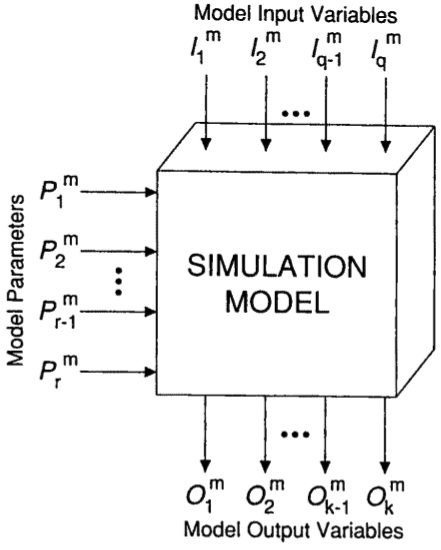
\includegraphics[width=.4\linewidth]{img/Balci1994a_Figure_Parametres.png}
	\caption{Les variables d'un modèle de simulation selon Balci \autocite[122]{balci_validation_1994}.\\
		\textit{Nota bene} : ce schéma est tronqué, ne présentant que la partie \og modèle de simulation\fg{} alors que celle-ci est mise en mirroir à une partie \og système\fg{} représentant l'empirique.}
	\label{fig:parametres-Balci} 
\end{figure}

Dans ce schéma et l'article associé, et bien qu'il n'en définisse nulle part explicitement le sens, Balci esquisse la composition d'un modèle de simulation.

\todobox{
		Décrire le schéma de Balci point par point. Faire un schéma pour Treuil, puis introduire les miens en les explicitant complètement.
		}


\subsubsection{Paramètres, variables, indicateurs : un essai de définition}
\label{subsubsec:mes_definitions_params}

Nous considèrerons donc plutôt les paramètres comme le sous-ensemble des entrées, qui peuvent s'exprimer sous forme numérique (excluant donc de fait certaines entrée telles que les configurations spatiales initiales), et que l'on fera varier, aussi bien dans la calibration du modèle que pour l'exploration de scénarios.


\todobox{
		Faire un schéma avec organisation des variables/paramètres/entrées/sorties telles que proposée dans ma thèse.
		}



\begin{figure}[!h]
	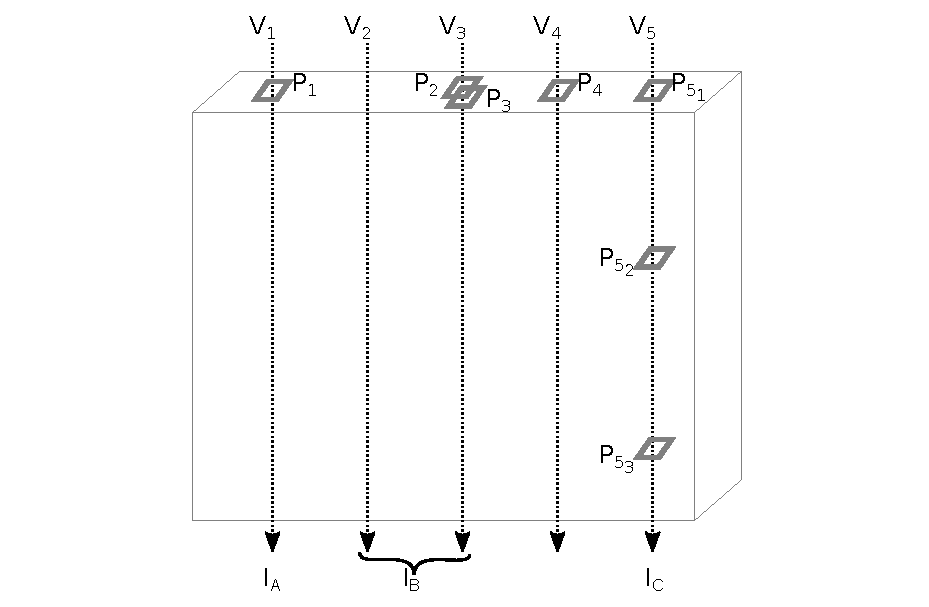
\includegraphics[width=\linewidth]{img/schemas_params_simple.pdf}
	\caption{Schématisation des définitions de variables (V), indicateurs de sortie (I) et paramètres (P).} 
	\label{fig:parametres-these-simple} 
\end{figure}

\colorbox{pink}{\parbox{0.9\textwidth}{%
		\vskip5pt
		\leftskip5pt\rightskip5pt
		Ne pas oublier de préciser différence entre paramètres et situation initiale. Ex. de situation initiale : des variables déjà allouées, par ex. pop des villes.
		Il n'y en a pas vraiment dans mon modèle pk tout est endogénéisé : pas de situation initiale, mais des paramètres qui définissent la création de celle-ci.
		\vskip5pt
	}
}

\begin{figure}[!h]
	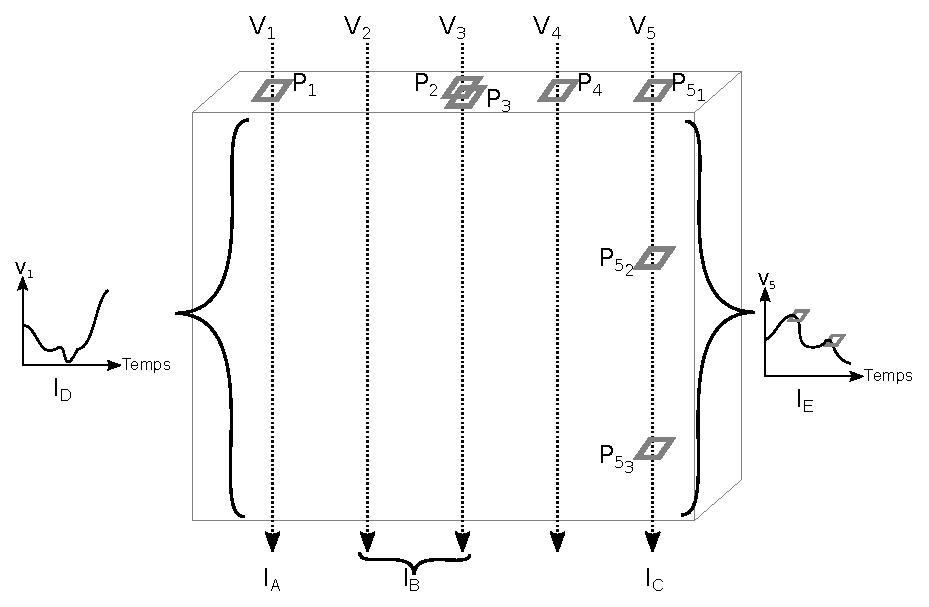
\includegraphics[width=\linewidth]{img/schemas_params_complet.pdf}
	\caption{Schématisation des définitions de variables (V), indicateurs de sortie (I) et paramètres (P) incorporant l'aspect temporel de certains indicateurs ($\text{I}_{\text{D}}$ et $\text{I}_{\text{E}}$).} 
	\label{fig:parametres-these-complet} 
\end{figure}

\newpage
\subsubsection{Paramètres et variables}

\begin{encadre}{Variables, entrées, paramètres\ldots}{termes-variables}
	Au sein des \textbf{variables}, constituées par l'ensemble des éléments d'un modèle ayant la capacité de changer, que ce soit au cours d'une simulation ou au travers de plusieurs expérimentations, nous distinguerons trois types spécifiques.
	\begin{description}[style=nextline]	
		\item[Entrées] Les \textbf{entrées} constituent l'ensemble des informations nécessaires à l'exécution d'un modèle en ce qu'elles en alimentent les mécanismes. Elles peuvent être constantes au cours d'une simulation (la date de fin d'exécution de notre modèle par exemple), ou évoluer de par l'action du modèle (le nombre d'églises paroissiale du modèle, qui est une entrée, et augmente tout au long de la simulation).
		
		\item[Paramètres] Certaines de ces entrées sont des \textbf{paramètres} : ce sont les entrées qui peuvent être mobilisées afin de modifier le comportement du modèle, et qui \og représentent ce que le simulateur peut perturber\fg{}\footnote{Pour reprendre les mots de Treuil et al. qu'ils appliquent aux entrées\autocite[8]{treuil_modelisation_2008}. }. Dans cet ouvrage, nous distinguerons plusieurs types de paramètres (\cref{enc:types-parametres}) selon leur ancrage dans l'empirique. Notons toutefois dès maintenant que le nombre de paramètres d'un modèle peut être bien supérieur au nombre de paramètres que l'on fera réellement varier dans les expérimentations.
		
		\item[Sorties] \hl{Les sorties d'un modèle représentent ce que l'on va observer après l'exécution du modèle afin d'observer son déroulement et aboutissement}.\footnote{Pas clair}.
		Ces sorties peuvent être très nombreuses, et concerner autant les variables individuelles (une liste des Foyers Paysans et de leur satisfaction au cours du temps par exemple) que des variables agrégées (Quartiles de satisfaction des foyers paysans par exemple), moins coûteuses en temps d'écriture ainsi qu'en espace de stockage. De la même manière que pour les paramètres, sur l'infinité potentielle de sorties d'un modèle, seules quelques-unes seront effectivement générées et enregistrées afin de minimiser les données produites à celles que le modélisateur compte explorer.
	\end{description}
\end{encadre}

\subsubsection{Différents types de paramètres}


Les paramètres sont donc un sous-ensemble des entrées d'un modèle qui ont vocation à varier dans les différentes exécutions de ce modèle. Pour autant, c'est un sous-ensemble assez divers, et tous les paramètres n'apportent pas les mêmes connaissances, que ce soit par leur valeur ou par la manière dont ils varient. Il convient donc d'identifier différents types de paramètres, non selon leur caractéristique propre (c'est-à-dire leurs propriétés, qui permettent de les différencier des sorties par exemple), mais selon leur usage et donc la manière dont on pourra les mobiliser. A ce titre, quand la littérature en sciences humaines et sociales\footnote{En physique ou en mathématiques par exemple, une telle distinction n'existe pas, la définition d'un paramètre prenant une considération plus simple d'élément rendu constant dans une exécution d'un modèle. \hl{pas clair, prendre une définition quelconque reprenant cette idée.}} distingue souvent (\hl{refs}) deux types de paramètres : les paramètres empiriques, dont la valeur a une correspondance directe dans le domaine empirique (on peut donc l'observer), et les paramètres techniques\footnote{Mathian et Tannier \autocite{mathian_formalisation_2015} utilisent le terme de paramètre mécanique pour définir ce type de paramètres. Nous trouvons l'usage du mot technique plus approprié, en ce qu'il se différencie plus de l'empirique sur le pan de l'usage qui en est fait. De plus, chaque paramètre, empirique, technique ou autre, a un impact sur les mécanismes du modèle, de par la définition que nous empruntons des paramètres \cref{enc:termes-variables}. Nous préférerons donc ce terme de \og technique\fg{} pour éviter les confusions.}, pour lesquels cette correspondance n'existe pas. Comme dans la plupart des typologies ayant trait à la catégorisation de valeurs numériques, de nombreux paramètres peuvent se trouver à l'interface de ces deux classes. Nous en proposons donc une troisième, que nous avons choisi de nommer \og paramètres commensurables\fg{}\footnote{
	La définition du dictionnaire \og Le Petit Robert\fg{} pour ce terme est celle-ci :  \og  Se dit d'une grandeur qui a, avec une autre grandeur, une commune mesure.\fg{}\autocite{robert_nouveau_1993}. \\Cf. aussi :			
	\og Les mondes n'apparaissent commensurables ou incommensurables qu'à ceux qui s'attachent aux mesures mesurées. Or, toutes les mesures, en science dure comme en science souple, sont aussi des mesures mesurantes et celles-là construisent une commensurabilité qui n'existait pas avant leur mise au point.\fg{}\autocite[153]{latour_nous_2013}},
qui nous semble à même caractériser des paramètres partiellement inscrits dans l'empirie, c'est-à-dire sans valeur empirique propre, mais permettant tout de même d'être mobilisés comme les paramètres empiriques, c'est-à-dire à même d'être comparés, que ce soit par les fluctuations de leurs propres valeurs ou en comparant des paramètres commensurables les uns avec les autres. Avec cette typologie des paramètres basées non sur la nature de ceux-ci mais sur leur utilisation dans un modèle, nous nous inscrivons dans une vision fonctionnaliste et donc très subjective, rappelant la définition d'un modèle de Minsky\footnote{\hl{Cf. sans doute le chapitre 1, à faire.}} \autocite{minsky_matter_1965}. Pour différents modélisateurs, un même paramètre pourra donc être considéré comme empirique ou commensurable, ou encore comme commensurable ou technique.
		\todobox{
		Ne pas oublier de préciser que selon le point de vue du modélisateur, un paramètre peut passer de empirique à commensurable, ou de commensurable à technique (et vice-versa), mais pas \og franchir\fg{} toutes les catégories.
		}


\begin{encadre}{Trois types de paramètres}{types-parametres}
	
	\todobox{
			Regarder s'il y a des enquêtes sur les seuils de satisfaction de Schelling dans la littérature.
	}
	
	\begin{description}
		\item[Paramètres empiriques] Les paramètres empiriques sont les paramètres qui peuvent être fixés à l'aide d'une ou de valeur(s) empiriquement connue(s), ou à défaut, dont la valeur se réfère à une quantité directement identifiable par une personne ayant des connaissances thématiques sur ce qui est modélisé.
		\begin{mdframed}[backgroundcolor=gray!10,footnoteinside=false]
			Dans le modèle de Schelling (\ref{desc:schelling}), le paramètre \fixref{\texttt{S}} est un paramètre empirique : la valeur qui lui est donnée peut être interprétée empiriquement, quand bien même il serait difficile d'obtenir, par exemple d'un enquêté, une valeur exacte à utiliser.
		\end{mdframed}
		\item[Paramètres techniques] Il s'agit des paramètres dont la valeur, ou même son ordre de grandeur, n'apportent aucune connaissance thématique au modélisateur. Ces paramètres ont pour raison d'être de permettre à d'autres types de paramètres de s'exprimer en valeurs compréhensibles et exploitables. Dès lors, leurs valeurs sont propres à chaque modèle formalisé, et une comparaison de ces valeurs entre les différents modèles n'apporte pas de connaissance.
		
		\begin{mdframed}[backgroundcolor=gray!10,footnoteinside=false]
			Dans le modèle gravitaire (\cref{desc:gravitaire}), $k$ est un paramètre technique : c'est un ratio qui varie afin d'ajuster l'ordre de grandeur des masses ($M_i$ et $M_j$) à celui des flux  échangés ($F_{ij}$). C'est une valeur d'ajustement, qui ne peut être comparée entre des modèles portant sur différents espaces et/ou thématiques\footnotemark.
		\end{mdframed}
		
		\item[Paramètres \og commensurable \fg{}]
		
		Cette catégorie, forgée dans le cadre de cet ouvrage, permet de représenter les paramètres qui ne sont pas fondamentalement issus de l'empirique mais qui peuvent toutefois être interprétés, que ce soit par rapport à une valeur canonique, définissant alors un repère, ou alors par rapport à d'autres valeurs de ce même paramètre, créant dès lors une échelle d'analyse. Outre la calibration d'un modèle, les valeurs de ces paramètres ont donc un intérêt propre et peuvent être analysées. pour elles-mêmes.
		
		\begin{mdframed}[backgroundcolor=gray!10,footnoteinside=false]
			Dans le modèle gravitaire (\cref{desc:gravitaire}), le frein de la distance (paramètre $\alpha$) peut être considéré comme un paramètre commensurable. Sa valeur ne renvoit ainsi à aucune dimension empirique, mais son usage répandu permet de comparer les valeurs qu'il peut prendre à des valeurs bien connues. Par exemple, on utilise fréquemment des valeurs de $\alpha$ comprises entre $1$ et $2$ pour exprimer la friction de la distance dans les navettes domicile-travail. Une valeur inférieure à $1$ peut donc être interprétée comme laissant une part plus faible à la distance, par exemple dans le cas de déplacements de loisirs. A contrario, un paramètre $\alpha$ supérieur à $2$ montrera une plus forte friction de la distance, par exemple dans les choix d'une école élémentaire à proximité du foyer d'un ménage.
		\end{mdframed}
	\end{description}
	\footnotetext{Dans le cas où $\alpha$ vaut $0$, ce paramètre peut être vu comme commensurable dans la mesure où il devient alors la part de la masse qui devient un flux.}
\end{encadre}


\subsubsection{Comment choisir les valeurs de paramètres ?}

\hl{Ici, faire un court paragraphe de transition pour présenter rapidement l'approche générale du paramétrage : peut-être redondant avec ce qui suit, en particulier dans les présentations des paramètrages du modèle gravitaire et de Schelling.}

\subsection{Le paramétrage, un processus d'amélioration du modèle.}

Le paramétrage d'un modèle est souvent réduit à l'un de ses aspects, le \og calibrage \fg, étape finale de la construction d'un modèle qui cherchera à reproduire autant que possible des données empirique en faisant varier les valeurs des paramètres jusqu'à ce qu'une combinaison de celles-ci soit satisfaisante.

De nombreux auteurs ont montré que le paramétrage d'un modèle ne pouvait se réduire à cette étape, chacun employant des termes différents pour désigner le processus de paramétrage.

%%%% Pas adapté  %%%%
Gilbert et Troitzsch \autocite{gilbert_simulation_2005} restent très flous en utilisant les termes de \textit{checking} et de \textit{debugging}, qu'ils inscrivent dans une démarche plus large de \textit{verification} correspondant à la \hl{validation interne}\footnote{\hl{Définir !}}.
Osman Balci \autocite{balci_validation_1994} crée et emploie l'acronyme \og \textit{VV\&T}\fg{}\footnote{\textit{Validation, Verification and Testing}}, à portée plus large puisqu'il s'applique à chacune des étapes de la modélisation
%%%%  %%%%

Le plus souvent (\fixref{ref Seb, Clem...}), une fois le modèle construit, le modélisateur s'attache à son \og calibrage\fg{}, en cherchant pour chaque paramètre la ou les valeurs qui permettront au modèle de s'approcher des données empiriques devant être reproduites.
Cette étape, que l'on nomme généralement calibration, peut se faire de manière manuelle, par approximations successives (\fixref{C. Cottineau et/ou S. Rey, d'après Hermann}), par semi-automatisme, \toChange{exemple en effectuant des analyses de sensibilité}{Lena : trouver d'autres exemples plus classiques et lointains} (\fixref{C. Schmitt, J. Hirtzel}), ou encore de manière entièrement automatique (\fixref{C. Schmitt, S. Rey, C. Cottineau avec PSE}).
L'approche souvent défendue, notamment dans les travaux les plus récents (\fixref{Rimbault?}), voudrait que cette étape soit obligatoire pour toute modélisation, permettant par une exploration systématique de comprendre l'entièreté du comportement d'un modèle, et d'en faire dès lors un outil complètement maitrisé \toChange{rendant possible l'établissement d'une loi}{Lena: expliciter}.

Dans notre travail, nous souhaitons revenir sur cette approche de la modélisation, ancrant le paramétrage comme étape ultime de la construction d'un modèle, en particulier en ce que nous considérons que cette pratique de recherches de \toChange{valeurs optimales}{Lena : penser à bien l'introduire avant.} est un exercice qui devrait s'effectuer tout au long de la construction du modèle, de manière plus itérative que conclusive.


\subsection{Qu'est-ce que le(s) paramétrage(s) ?}

\subsubsection{Définition}

\toChange{Paramétrer (informatique): \og Programmer (un appareil complexe), en définissant les paramètres assurant son fonctionnement optimal. Ex. \textit{Paramétrer une imprimante}\fg{}\autocite{robert_nouveau_1993}.}{J'aime bien cette définition, c'est la seule à avoir le sens que j'entends dans paramétrage/paramétrer. Et elle introduit une logique d'optimalité.}

Le terme recouvre deux sens différents, dont la distinction peut se faire selon qu'on l'utilise pour définir un processus ou pour caractériser une configuration.
Ici, nous emploierons plutôt le premier cas, définissant dès lors le paramétrage comme le processus, manuel ou automatique, visant à constituer cette configuration de paramètres.
Dans ce deuxième cas, le paramétrage désigne un ensemble de valeurs de paramètres, par exemple quand on mentionne un paramétrage par défaut, ou un paramétrage optimal.
Pour ne pas risquer de contre-sens, nous préférerons le terme de configuration de paramètres.

On tend à distinguer le paramétrage -- passage obligé ne nécessitant pas d'être évoqué -- de la calibration, processus systématique qui inscrirait le modèle comme un outil scientifique et incontestable.
Nous choisissons ici de confondre ces approches, non pas en considérant le paramétrage comme un outil d'évaluation du modèle, mais comme une composante inhérente à la construction d'un modèle, quelque soient les formes et les temporalités que le paramétrage adopte.
Le paramétrage est en effet une pratique utile dans la construction du modèle, car les résultats auxquels il aboutit, c'est-à-dire les valeurs de paramètres qui semblent mieux adaptés, renseignent aussi bien sur les biais des mécanismes adoptés que sur leur efficacité réelle.
Par exemple, quand, après avoir ajouté un mécanisme, on se rend compte que des variations dans les valeurs de paramètres ne changent pas réellement les sorties du modèle, cela peut être l'occasion de repenser le mécanisme dans son ensemble, ou plus souvent, la manière dont le paramètre est mobilisé dans ce mécanisme. On retrouve cette logique dans l'exploration par Clara Schmitt du modèle SimpopLocal \autocite{schmitt_modelisation_2014}, qui a permis de réaliser que la variation de l'un des paramètres ($InnovationLife$) n'avait que peu d'impact sur les sorties du modèle, tout en rendant sa calibration plus complexe et instable :
\begin{quote}
	Au dessous du seuil des 150 pas de simulation pour le paramétrage de InnovationLife, le calibrage du modèle est très difficile voire impossible. Au dessus de ce seuil, le mécanisme associé au paramètre InnovationLife n’a plus d’effet sur le calibrage du modèle. Dans un soucis de parcimonie du nombre et de la complexité des mécanismes simulés dans le modèle SimpopLocal, il est justifiable de retirer du modèle ce mécanisme qui n’est pas nécessaire à la simulation de la dynamique de croissance recherchée.\\
	\mbox{}~ \hfill \autocite[224]{schmitt_modelisation_2014}
\end{quote}

\paragraph{}Afin d'illustrer ces propos, on peut s'appuyer sur des modèles bien connus de la littérature, issus de deux champs disciplinaires différents.

\subsubsection{Illustration : le modèle gravitaire.\label{desc:gravitaire}}

\paragraph{Description}	Ce modèle statistique\footnote{Pour une description plus complète, se référer à l'ouvrage de Pumain et Saint-Julien \autocite{pumain_les_2001}.}, dans la formulation qu'en a faite Stewart \autocite{stewart_demographic_1948}, vise à prédire des flux (démographiques, marchands etc.) potentiels entre des lieux à partir d'une analogie avec la loi physique de la gravitation. Dans le formalisme le plus simple, \og sans contrainte\fg{} \autocite{pumain_les_2001}, on peut l'exprimer ainsi :
$$
F_{ij} = \frac{k \times M_{i} \times M_{j}}{d_{ij}{}^\alpha}
$$
Ce modèle présente trois valeurs empiriques ($M_i$, $M_j$ et $d_{ij}$) et deux paramètres ($k$ et $\alpha$). $k$ est un paramètre technique (\cref{enc:types-parametres}), puisque bien que basée sur l'empirique, sa valeur -- et les fluctuations de celle-ci -- ne donne aucune information sur le système étudié. $\alpha$ est un paramètre commensurable pour les raisons explicités dans l'\cref{enc:types-parametres}.

À partir des valeurs empiriques $M_i$ et $M_j$ qui caractérisent les masses (populations, ou stocks de  marchandise par exemple) des lieux $i$ et $j$, et de la distance qui les sépare $d_{ij}$, on peut ainsi prédire $F_{ij}$, le flux entre ces lieux.

\paragraph{Objectif} Afin que ce modèle donne des ordres de grandeur réalistes quand aux quantités échangées, il faut le paramétrer en définissant une valeur de $k$, permettant dès lors d'obtenir un rapport entre les masses d'origine et les quantités échangées.
La valeur de ce paramètre est conditionnée par celle de $\alpha$, que l'on nomme fréquemment \og frein de la distance\fg{}, en ce qu'il permet de quantifier l'impact qu'aura un éloignement plus ou moins important sur la quantité de flux échangés.

\paragraph{Paramétrage} Pour \og ajuster\fg{}\footnote{C'est le terme employé par \autocite{pumain_les_2001}, que l'on peut ici retenir comme équivalent de paramétrer. François Durand-Dastès  \autocite[298]{durand1995modeles} utilise pour sa part le terme de calibration à propos du même modèle.} le modèle, il faut donc en réaliser le paramétrage en s'appuyant sur les éléments connus de l'équation (les valeurs empiriques).
$\alpha$ et $k$ étant liés dans l'équation, la valeur de chacun de ces paramètres dépend de celle choisie pour l'autre, et un changement dans l'un des paramètres entraînera la nécessité de modifier l'autre.

Le paramétrage le plus simple consiste à réaliser une régression linéaire sur les logarithmes décimaux des distances et des flux observés, $k$ prenant alors la valeur du logarithme de l'ordonnée à l'origine et $\alpha$ celle du coefficient directeur de la courbe.	
Le modèle est alors calibré (voir \cref{enc:termes-calibration}), mais si l'on souhaite donner une valeur spécifique à l'un des paramètres, par exemple pour utiliser une valeur classique de 2 au frein de la distance ($\alpha$) \autocite{pumain_modegravitaire_2004}, il faudra alors le re-soumettre à paramétrage pour adapter $k$. De même si l'on modifie les lieux et/ou les masses sur lesquels il s'applique.


\subsubsection{Illustration : le modèle de ségrégation de Schelling.\label{desc:schelling}}

\paragraph{Description}Le modèle de Schelling\footnote{Une description plus poussée accompagnée d'une description de l'exploration du modèle peut être lue dans \autocite{daude_comparaison_2006}} est un modèle de simulation décrit par Thomas Schelling \autocite{schelling_dynamic_1971} qui vise à montrer comment un espace peut passer d'un état intégré à un état ségrégé ethniquement à travers une succession de comportements individuels de mobilité résidentielle. Il montre en particulier qu'on peut parvenir à un état ségrégé même quand les comportements individuels sont majoritairement tolérants.

L'espace du modèle est défini comme une grille carrée composée de $N$\footnote{Nous reprenons ici la notation $M(N, d, n, S)$ proposée par \autocite[433]{daude_comparaison_2006} en n'explicitant toutefois pas le paramètre $n$ décrivant le type de voisinage (4 ou 8) utilisé.} cellules.
Au début de la simulation, des agents de deux types, en proportions similaires, sont distribués aléatoirement dans l'espace du modèle. Chaque agent occupe une cellule, et le nombre total de cellules occupées (et donc d'agents) dépend d'un paramètre de densité $d$ qui représente la part (entre $0\%$ et $100\%$) du nombre de cellule qui sera occupé\footnote{Il y a donc $N \times d$ agents, et donc $\frac{N \times d}{2}$ agents de chaque type.}.
Chaque agent est défini par une satisfaction. Celle-ci correspond à la part de cellules voisines occupées par des agents \og étrangers\fg{}, c'est-à-dire d'un autre type : plus le voisinage contient d'étrangers, moins l'agent est satisfait.
Si cette satisfaction est inférieure à un paramètre de tolérance $S$, l'agent est considéré comme insatisfait et se déplace aléatoirement dans une cellule non occupée.
A terme, Schelling montre que même en considérant des valeurs de $S$ assez élevées, c'est-à-dire un comportement plutôt tolérant, la succession de choix individuels entraîne la mise en place d'une distribution spatiale très ségrégée.
On considère que le modèle a convergé quand l'ensemble des agents sont satisfaits, ce que ne permettent pas toutes les combinaisons de valeurs de paramètres.

Dans ce modèle, on peut donc dénoter trois paramètres, $N$, $d$ et $S$. Les deux premier sont des paramètres techniques (\cref{enc:types-parametres}), en ce que, purement théoriques, ils ne se réfèrent à aucune quantité empirique, ni ne peuvent être utilisés afin de se référer à un ordre de grandeur connu qui en ferait des paramètres commensurables. $S$ est un paramètre empirique. Bien que le modèle soit théorique, ce paramètre se réfère toutefois à une comportement ayant un sens empirique fort.

\paragraph{Objectif} Le paramétrage de ce modèle consiste à fixer un $N$ constant et à faire varier $d$ et $S$ afin d'en trouver des valeurs permettant la convergence vers une situation stable. Quand $d$ est très faible ($30\%$ dans l'exemple de \autocite{daude_comparaison_2006}), quelles que soient les valeurs de $S$, le modèle converge rapidement : quand l'espace du modèle dispose d'une faible densité d'agents, il est facile pour ceux-là de créer des agrégats homogènes distants d'agrégats de l'autre type d'agents. Quand $d$ est plus important ($\geq66\%$), l'espace disponible étant limité, toutes les valeurs de $S$ ne permettent pas la convergence du modèle. Le paramétrage du modèle aura donc pour objectif de trouver la valeur maximale possible -- pour un $N$ et un $d$ donné -- que peut prendre le paramètre de tolérance $S$ tout en laissant le modèle converger.

\paragraph{Paramétrage}Contrairement au modèle gravitaire, le modèle de Schelling est stochastique : les agents se déplacent aléatoirement quand non satisfaits. Dès lors, deux exécutions du modèle avec le même jeu de paramètres n’entraîneront pas forcément la même configuration spatiale. Qui plus est, pour certains jeux de paramètres, seules certaines exécutions convergeront. Le paramétrage de ce modèle ressemble donc à celui qui est réalisé pour le modèle SimFeodal. La manière \og traditionnelle\fg{}\footnote{C'est-à-dire manuelle, au contraire de méthodes automatiques plus rigoureuses et récentes.} consiste à fixer un $d$, puis à essayer d'augmenter le $S$ tant que le modèle converge. Si le modèle converge pour tout $S$, on augmente la valeur de $d$ et on recommence à chercher la valeur maximale possible pour $S$. De part la nature stochastique du modèle, chaque jeu de paramètres doit être simulé plusieurs fois, le nombre de ces réplications dépendant de la part d'aléa dans le comportement du modèle.
Un modèle de Schelling calibré, c'est-à-dire dont le paramétrage est achevé,
donnera pour un $N$ fixé les valeurs maximales de $d$ et de $S$ atteignables.

\paragraph{}A travers ces deux exemples ayant traits à des méthodes différentes, on retrouve deux approches de paramétrage que l'on souhaite ici voire confondues : dans le premier cas, le paramétrage du modèle gravitaire tend à sa calibration, à la recherche d'une solution optimale, c'est-à-dire meilleure que toute autre. Pour un phénomène donné (un jeu de données précis par exemple) et un formalisme donné (l'expression la plus simple du modèle, ici sans contrainte), seule un couple de paramètres $\alpha$ et $k$ permet ainsi d'obtenir des flux modélisés proches des flux observés.
Dans le cas du modèle de Schelling, il n'y a pas de recherche d'optimum : le paramétrage permet de comprendre le modèle en en définissant les limites en matière de convergence. Une configuration de paramètres $S$ et $d$ ne sera pas meilleure qu'une autre, mais pour un $S$ donné, on saura quel est la valeur maximale de $d$ permettant cette convergence (et réciproquement).

\subsubsection{Paramétrer un ou des modèles ?}

\toChange{\fixref{Cottineau, Reuillon et Rey} ont montré qu'on construisait plus souvent des familles de modèles que des modèles uniques.}{Lena : trop endogame, prendre exemples modèles modulaires dans JASSS}
Ces auteurs plaident pour une construction modulaire de modèles, chacun des mécanismes et complexifications devant être autonomes afin de pouvoir les assembler en autant de combinaisons que nécessaire à une exploration d'ensemble de leurs interactions.

Nous reprendrons de leur discours une vision moins ambitieuse, en considérant (\toChange{ref Rey}{à chercher il en parlait à sa soutenance je crois}) simplement qu'en fait d'un modèle, la modélisation passe par plusieurs modèles, ayant chacun différentes implémentations d'un mécanisme conceptuellement identique et chacun se devant dès lors d'être adapté par un paramétrage dédié.

Pour illustrer ce propos, on peut prendre l'exemple d'une modification qui a eu lieu sur notre modèle au cours de son développement. On considérait jusque là que pour prendre en compte la population rurale (hors Tours donc), $1000$ foyers paysans donnaient une bonne idée de la situation en 800 pour l'espace considéré.
Lors d'une réunion, les thématiciens se sont rendus compte que ce nombre sous-estimait très largement la population réelle, et qu'il valait mieux passer ce paramètre à $4000$ foyers paysans.
Les autres paramètres, fixés en bonne partie empiriquement, n'avaient visiblement aucune raison d'évoluer du fait de ce changement. Les mécanismes  et effets de seuil étaient en effet conçus de manière à être relatifs aux masses manipulées, et le changement attendu était une augmentation linéaire des indicateurs de sortie.

\begin{figure}[H]
	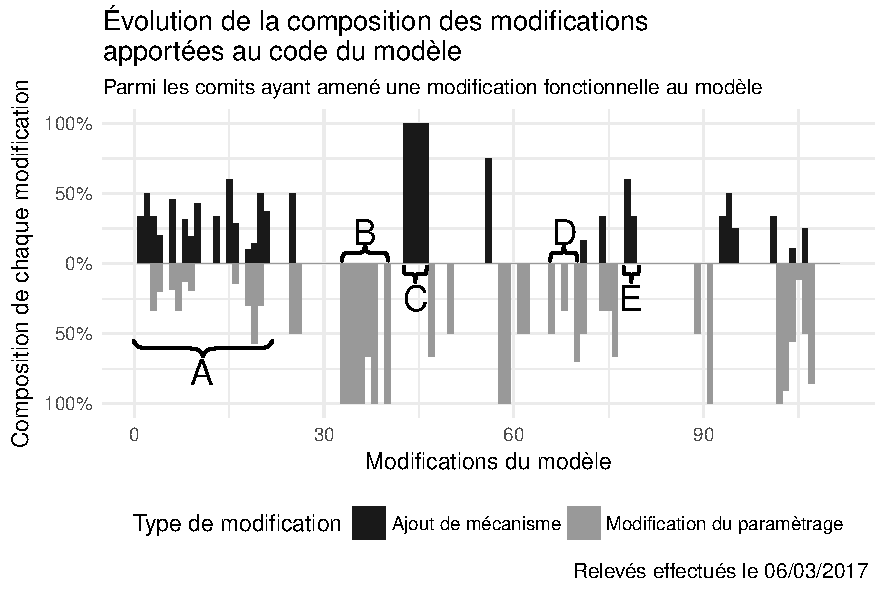
\includegraphics[width = \linewidth]{img/plotComits.pdf}
	\caption{Temporalité du paramétrage du modèle.\\
		Chaque \og enregistrement\fg{} (\textit{comit}) correspond à une version modifiée et sauvegardée du modèle, contenant un ou plusieurs changements. On a ici rapporté le nombre de changements de chaque type (modification de mécanisme ou de valeur de paramètre) au nombre total de changements de chaque \textit{comit} afin de figurer l'évolution des types de modification au cours de la construction du modèle.}
	\label{fig:comits-periodes}
\end{figure}

Dans les faits, cette légère modification a entraîné une obligation de repenser la quasi-totalité des autres paramètres et d'ajuster une bonne part des règles. 
La concentration des foyers paysans était en effet bien trop rapide avec autant d'individus, et le modèle convergeait en quelques pas de temps vers une configuration presque statique et très concentrée.
Tous les mécanismes de régulation de ce comportement étaient dès lors rendus ineptes, et il a fallu changer en profondeur la manière dont chaque paramètre et mécanisme interagissait avec les autres.
\toChange{C'est un changement majeur, que l'on peut constater dans la figure~\ref{fig:comits-periodes} (1ère modification de la période B), ayant donc entraîné des adaptations de tous les plans du modèle (paramètres en B, mécanismes en C).}{Lena : Là on ne suit pas, mais ce sera explicité dans le chap. 2}
La première version avait été paramétré aussi correctement que possible, mais ce paramétrage était entièrement à refaire avec la nouvelle version (modifications de la période B, \cref{fig:comits-periodes}).
\toChange{On pourrait dès lors différencier le modèle pré-existant et celui qui a suivi ce changement, et les considérer comme deux modèles puisque réagissant de manière extrêmement différente.}{Lena : à discuter plus profondément}

\toChange{Cet exemple renforce le caractère nécessaire du paramétrage, et qui plus est, de la continuité de cette étape, qui ne peut être pensée que comme une calibration finale d'un modèle abouti, auquel on ne peut en fait parvenir que par des paramétrages réguliers de modèles successifs moins aboutis.}{Lena: Pas clair et pas assez logique}

\subsubsection{Désambiguïsation}

De nombreux termes sont utilisés dans la littérature, souvent sans réelle distinction, pour désigner cette opération qui consister à choisir un jeu de paramètres pour un modèle. Pêle-mêle, on y retrouve le paramétrage, la validation, l'évaluation ou encore la calibration. Nous définissons dans l'\cref{enc:termes-calibration} le sens donné à chacun de ces termes dans le cadre de ce manuscrit.
\bigskip

\begin{encadre}{Calibration, évaluation, validation\ldots}{termes-calibration}
	\begin{description}[style=nextline]	
		\item[Calibration] On réserve souvent, et nous nous y tiendrons, ce terme à la dernière étape dans l'aboutissement d'un modèle.
		Une fois les mécanismes fixés et des objectifs définis, on peut procéder à la calibration, c'est-à-dire à une exploration de l'espace des paramètres ayant pour but de stabiliser les paramètres afin de se rapprocher autant que possible de ces objectifs.
		Cette étape, quelques soient les moyens employés, s'approche de la résolution utilisée dans le cadre de systèmes d'équations.
		Le contexte des systèmes complexes, et donc d'une non-linéarité des effets des paramètres, rend toutefois difficile l'obtention d'une unique configuration de \hl{paramètres optimale}\footnote{Lena : il faut partir d'une def plus basique en intro}, et la calibration aboutit donc souvent à un ensemble de configurations possibles, constituant par exemple un optimum de Pareto (\fixref{Trouver ref}).
		
		\item[Évaluation] On emploie majoritairement ce mot pour décrire les méthodes permettant de comprendre le comportement du modèle et sa réaction aux différents paramètres.
		Là où la calibration cherche une configuration de paramètres optimale, l'évaluation tend surtout à caractériser la stabilité du modèle face à l'aléa ou a des configurations exceptionnelles.
		On vise ainsi à s'assurer que le modèle reproduise \hl{les faits stylisés}\footnote{Lena : pas introduits avant} voulus quelque soient son réglage, ou au moins à quantifier les intervalles de paramètres qui y satisfont.
		
		\item[Validation] La validation (refs Seb) tire son origine de sciences plus nomothétiques, et correspond donc à la démonstration qu'un modèle reproduit correctement ce qu'il représente. Au delà de l'évaluation, le terme amène une logique de preuve formelle que le modèle réagit bien ainsi et pas autrement quelque soient les conditions d'exécution. Cette démonstration formelle peut être effectuée sur des modèles à faible nombre de paramètres et mécanismes, mais le terme n'est jamais (à vérifier) employé dès lors que les modèles se complexifient.\footnote{Lena : cf. JASSS : Faire un rappel du sens classique, par ex. en stats.}
	\end{description}
\end{encadre}




\clearpage
\section{Paramétrage de SimFeodal}
	
\subsection{Avant propos sur le paramétrage d'un modèle complexe}
	
	\todobox{
	A changer : le chap 2 présentera la version 0 (Base) du modèle, et on vient donc ici montrer comment on a répondu aux limites identifiées à la fin du chapitre, cf. les conclusions/résultats du chapitre TransMonDyn.
	}
\medbreak
	
	\todobox{
	Pour introduire le schéma des étapes, rappeler ici que les paramètres et mécanismes d'un modèle complexe sont en interaction, ce qui produit des effets non linéaires.\\
	Principe des vases communicants !\\
	Mentionner aussi la logique des attracteurs étranges de Lorenz comme paroxysme de cette complexité : ici, moins de variation, mais des répercussions importantes tout de même qu'il faut donc \og corriger\fg{} par de nombreuses itérations de modifications.
	}

Le tableau suivant (\cref{table:etapes-construction}) se veut être un point de repère autant qu'une table des matières synthétique pour la compréhension des étapes qui suivent. Si la description de chacune de celles-ci revêt une forme assez factuelle et systématique, nous pensons toutefois que l'explicitation de chacune de ces étapes permet de saisir la démarche proposée ainsi que l'intérêt de celle-ci.

Notons que l'étape 0 ici présentée correspond à une première version \og exploitable\fg{} du modèle, c'est-à-dire contenant \textit{a minima} l'ensemble des agents et mécanismes identifiés dans un premier temps par l'équipe de modélisation \autocite{tannier_ontologie_2014}. Nous ne détaillerons pas ici les différentes phases de construction précédentes. Nous reviendrons toutefois sur plusieurs d'entre elles, en guise d'exemples illustratifs, dans les chapitres 6 et 7 \hl{(Partie 3)}.

\subsubsection{De manière générale}
	
\subsection{Les étapes du paramètrage de SimFeodal}
	
Comme préconisé ci-dessus, le modèle SimFeodal a été paramétré tout au long de sa construction. Dans cette partie, nous reviendrons en détail sur chacune des étapes de ce paramétrage, en retraçant les choix et questionnements qui ont orienté ces modifications du modèle. L'énumération est en ordre chronologique, et l'on a essayé d'organiser ces étapes en grands blocs-type de paramétrisation. Pour autant, le paramétrage et la construction d'un modèle, et du notre en particulier, sont un travail constant d'allers-retours entre l'identification et la résolution de problèmes. La structure réelle de développement, que l'on peut retrouver dans l'historique des modifications du modèle (les \og \textit{commits}\fg{}), ne correspond donc pas exactement à la chronologie organisée qui suit.
	
	
\pagebreak
\begin{footnotesize}
	\begin{longtable}{ m{.05\textwidth} m{.08\textwidth}  m{.12\textwidth}  m{.65\textwidth}  m{.10\textwidth}  }
		\caption{Tableau récapitulatif des étapes de construction du modèle. Conception : C. Tannier (\fixref{Tannier 2017, HDR}) et R. Cura, 2017}\\
		\label{table:etapes-construction}\\
		Étape & Version & Type      & Modifications                                                 & Section                                                                                   \\
		\endfirsthead
		Étape & Version & Type      & Modifications                                                 & Section                                                                                   \\
		\endhead			
		\hline
		0      & Base    & Création & Création du modèle. \fixref{Cf. tableau 14 de Tannier 2017} & Chap 2\footnote{On s'appuie sur cette version \og Base\fg{} dans le \fixref{chapitre 2}.} \\
		\hline
		1 & Base2 & paramétrage & \colorbox{yellow}{Hiérarchisation} des valeurs d'attraction des attracteurs. \newline
		Modification des critères de création de nouvelles paroisses. \newline
		Réduction de la distance maximale de déplacement local. \newline
		Assouplissement des règles de promotion d'un château en gros château. & Chap3-x.y\\
		\hline
		2 & Base2 compo5 2bis & modélisation et paramétrage & Assouplissement des règles de création d'une paroisse.\newline
		Réduction de la distance maximale de déplacement local. \newline
		Modification des règles de calcul de la probabilité de construire un château.\newline
		Modification du calcul de la satisfaction matérielle des foyers paysans. & Chap3-x.y\\
		\hline
		3 & Base2 compo5 2quat & modélisation et paramétrage & \colorbox{yellow}{Hiérarchisation} des valeurs d'attraction des attracteurs. \newline
		Facilitation de la construction de châteaux. \newline
		Rationnalisation du déplacement des foyers paysans. \newline
		Ajout d'un nouveau type d'attracteur, les communautés. & Chap3-x.y\\
		\hline
		4 & Base3 2 & modélisation et paramétrage & \colorbox{yellow}{Hiérarchisation} des valeurs d'attraction des attracteurs. \newline
		Modification des critères de création de nouvelles paroisses. \newline
		Augmentation de la distance maximale de déplacement local. \newline
		Modification de la procédure d'identification des agrégats et des pôles. & Chap3-x.y\\
		\hline
		5 & Base4 1 & modélisation et paramétrage & 
		Modification de la répartition initiale des foyers paysans.\newline
		Simplification de la procédure d'identification d'héritage des agrégats.
		Amélioration de la définition des pôles d'attraction et de leur enveloppe. & Chap3-x.y\\
		\hline
		6 & Base4 2 & modélisation et paramétrage & \colorbox{yellow}{Hiérarchisation} des valeurs d'attraction des attracteurs. \newline
		Modification de l'ordonnancement des actions dans le modèle.\newline
		Modification de la procédure d'identification des agrégats. & Chap3-x.y\\
		\hline
		7 & Base4 3ter & modélisation et paramétrage &
		Dynamisation de la distance maximale de déplacement local.\newline
		Modification du calcul de satisfaction des foyers paysans. & Chap3-x.y\\
		\hline
		8 & Base4 4A & modélisation & Modification de l'ordonnancement des actions dans le modèle.\newline
		Modification du mécanisme de déplacement local des foyers paysans. & Chap3-x.y\\
		\hline
					
	\end{longtable}
\end{footnotesize}

\subsubsection{Étape 0}
	
\paragraph{Indicateurs généraux}
	
\begin{table}[H]
	\centering
	\caption{Indicateurs synthétiques de l'étape 1}
	\label{my-label}
	\begin{tabular}{lll}
		Indice             & Objectif & Moyenne \\
		Nb agrégats       & 200.00   & 145.30  \\
		Nb châteaux       & 50.00    & 69.78   \\
		Nb gros  Châteaux & 10.00    & 9.60    \\
		Nb egl. Par.       & 300.00   & 167.90  \\
		Dist entre égl.   & 3000.00  & 2944.00 \\
		FP isolés         & 0.20     & 0.49    \\
		Ratio Charge Fisc. & 3.00     & 5.15    
	\end{tabular}
\end{table}

\pagebreak
\subsubsection{Étape 1}
\begin{figure}[H]
	\centering
	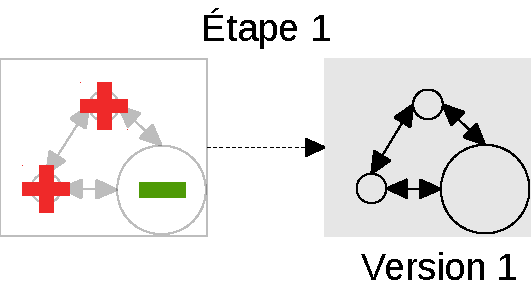
\includegraphics[width = \linewidth, page = 1]{img/schemas_etapes_individuelles.pdf}
	\caption{Étape 1 du paramétrage et résultats.}
\end{figure}

\pagebreak
\subsubsection{Étape 2}
\begin{figure}[H]
	\centering
	\includegraphics[width = \linewidth, page = 2]{img/schemas_etapes_individuelles.pdf}
	\caption{Étape 2 du paramétrage et résultats.}
\end{figure}

\pagebreak
\subsubsection{Étape 3}
\begin{figure}[H]
	\centering
	\includegraphics[width = \linewidth, page = 3]{img/schemas_etapes_individuelles.pdf}
	\caption{Étape 3 du paramétrage et résultats.}
\end{figure}

\pagebreak
\subsubsection{Étape 4}
\begin{figure}[H]
	\centering
	\includegraphics[width = \linewidth, page = 4]{img/schemas_etapes_individuelles.pdf}
	\caption{Étape 4 du paramétrage et résultats.}
\end{figure}

\pagebreak
\subsubsection{Étape 5}
\begin{figure}[H]
	\centering
	\includegraphics[width = \linewidth, page = 5]{img/schemas_etapes_individuelles.pdf}
	\caption{Étape 5 du paramétrage et résultats.}
\end{figure}

\pagebreak
\subsubsection{Étape 6}
\begin{figure}[H]
	\centering
	\includegraphics[width = \linewidth, page = 6]{img/schemas_etapes_individuelles.pdf}
	\caption{Étape 6 du paramétrage et résultats.}
\end{figure}

\pagebreak
\subsubsection{Étape 7}
\begin{figure}[H]
	\centering
	\includegraphics[width = \linewidth, page = 7]{img/schemas_etapes_individuelles.pdf}
	\caption{Étape 7 du paramétrage et résultats.}
\end{figure}

\pagebreak
\subsubsection{Étape 8}
\begin{figure}[H]
	\centering
	\includegraphics[width = \linewidth, page = 8]{img/schemas_etapes_individuelles.pdf}
	\caption{Étape 8 du paramétrage et résultats.}
\end{figure}
	
\pagebreak
\subsection{Un bilan des changements majeurs à l'issu du paramétrage}
	
\begin{figure}[H]
	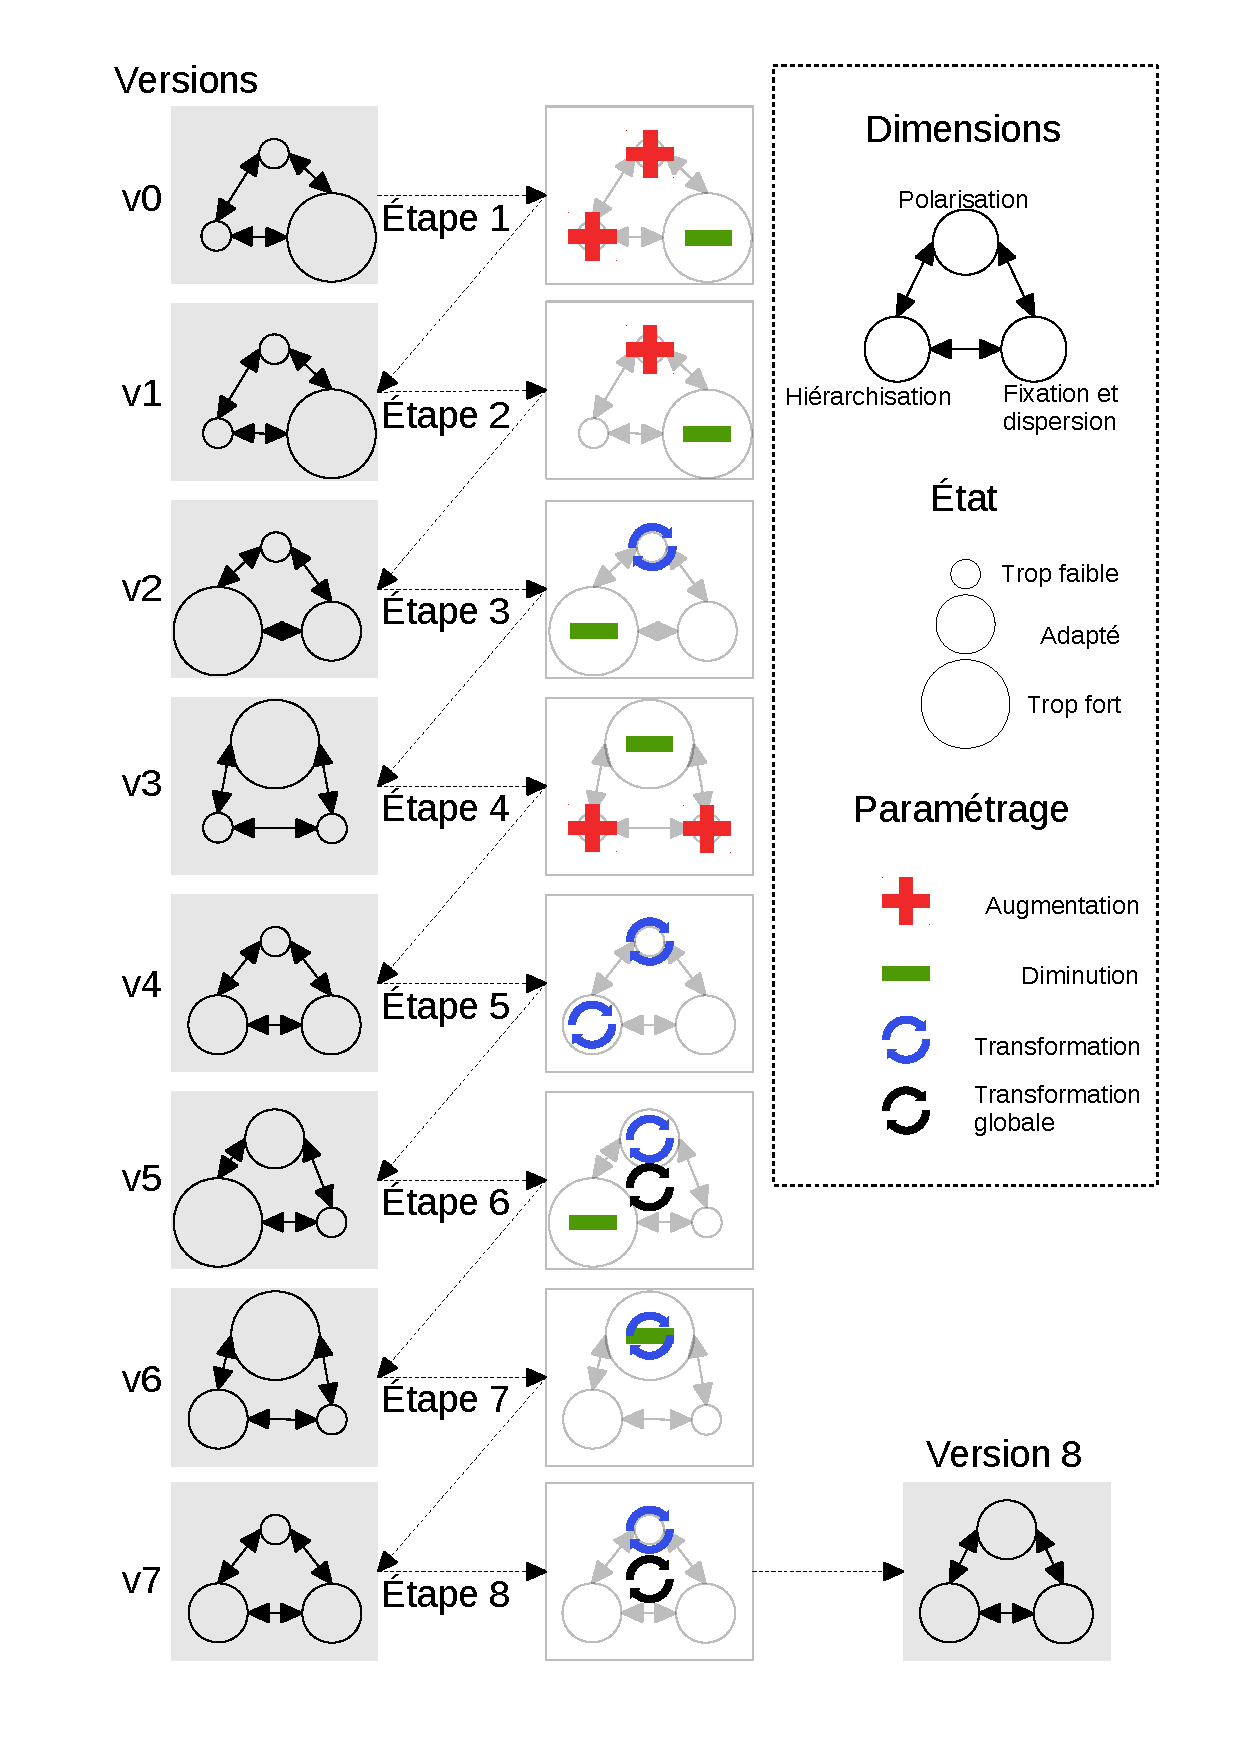
\includegraphics[width = \linewidth, page = 1]{img/schema_etapes_complet.pdf}
	\caption{Schéma récapitulatif et synthétique des étapes du paramétrage de SimFeodal.}
	\label{fig:etapes-parametrage-simfeodal}
\end{figure}
	

\clearpage
\section{Comment traiter les sorties du modèle ?}
\subsection{Variabilité}
- Quelle variabilité du modèle ? Pour quelles raisons (aléa init. vs aléa mécanique) ?
\subsection{Nombre de sortie}
- Sorties graphiques, rapports, rapports ++
\subsection{Masse des sorties}
- Comment aller plus loin ?


%	\printbibliography 

%
%\setcounter{part}{1}
%\part{L'analyse visuelle exploratoire au service de la compréhension de phénomènes spatiaux} 
%
%\graphicspath{{chap5/}}
%\setcounter{chapter}{4}
%% !TEX root = ../These_Robin_Master.tex
\chapter{Explorer visuellement des données de simulation massives pour analyser le comportement d'un modèle.}
\label{chap:chap5}
\begin{center}
{\large Version \hl{2019-05-09}}

\end{center}
\minitoc

%\setcounter{section}{0}
%\clearpage
\section*{Introduction}
\addcontentsline{toc}{section}{\protect\numberline{}Introduction}
%TODO : Ecrire introduction
\hl{A faire}\\
-> Définir notamment la démarche : contraintes générales -> spécificités SimFeodal -> choix méthodos/techniques

%\setcounter{section}{0}
%\clearpage
\section[Capter les sorties de SimFeodal]{{Capter les sorties de SimFeodal}%
	\sectionmark{Capter les sorties}}\label{sec:sorties-simfeodal}
\sectionmark{Capter les sorties}

Pour évaluer un modèle, on s'appuie sur plusieurs indicateurs de sortie de simulation, de types divers (indicateurs numériques, graphiques, cartographiques etc., \hl{cf. chapitre 3, partie théorique}).
Quand le nombre d'indicateurs devient important, comme c'est le cas dans le modèle SimFeodal (chap 3, partie présentation des indicateurs), la consultation des indicateurs pendant le déroulement d'une simulation devient difficile.
La complexité de ces indicateurs augmente dans le cas d'un modèle stochastique comme SimFeodal, où il est nécessaire de multiplier les réplications afin d'avoir une idée fiable des tendances simulées par le modèle.
Le travail de paramétrage d'un modèle requiert de plus de mener différentes expériences, c'est-à-dire de faire varier les paramètres (chap 4) du modèle, démultipliant encore la masse des sorties, et avec elle, la complexité de leur analyse.
Nous détaillons ici les contraintes qu'entraînent ces différentes spécificités des données issues des simulations de SimFeodal.

	\subsection{Masse des données}
	Dans un premier temps, il convient de noter que l'ensemble des indicateurs observés en sortie de SimFeodal reposent sur des données qu'il est nécessaire de produire et d'enregistrer tout au long de la simulation.
	Ainsi, pour pouvoir tracer une courbe de l'évolution du nombre d'agrégats au cours du temps, il faut avoir accès à cette information, et dès lors, enregistrer, à chaque pas de temps, cette valeur dans un fichier numérique adapté.
	Cette information, en tant que telle, est assez faible, aussi bien en valeur sémantique qu'en valeur prise en mémoire.
	Pour autant, on a montré que les indicateurs de sortie étaient nombreux, et avec eux, la quantité de valeurs à stocker augmente.
	Ainsi, à chaque pas de temps, il faudra enregistrer les valeurs de plusieurs variables.
	Cette pratique est habituelle, et un format de données tabulaire se prête bien à un tel enregistrement : une ligne pour chaque pas de temps, et une colonne pour chaque variable à enregistrer.
	On obtiendrait ainsi en sortie de simulation un tableau contenant 18 lignes (le nombre de pas de temps de SimFeodal, cf. \hl{chap2, faire référence à page}) et une cinquantaine de colonnes, ce qui serait assez raisonnable.

	Il faut toutefois prendre en compte un aspect important de l'exploration de données issues de simulations : la production de ces données a un coût temporel important, c'est-à-dire que l'exécution d'une simulation requiert un certain temps (3 à 4 minutes pour une exécution du modèle SimFeodal dans la version présentée dans le \hl{chapitre 2}).
	
	Avec la démultiplication des expériences et la nécessaire évolution du modèle au fur et à mesure de son évolution, il peut être extrêmement difficile, long et fastidieux de ré-exécuter l'ensemble des simulations précédemment effectuées.
	Les indicateurs peuvent évoluer au cours du temps de vie du modèle (cf. \hl{encadré chap 3}), ou plus simplement, on peut être amené à réaliser une observation plus fine des sorties du modèle au fur et à mesure de la calibration de ce dernier.
	Par exemple, parmi les indicateurs de sortie de SimFeodal, on s'intéresse notamment à la composition des pôles, que l'on qualifie assez simplement d'une part avec le nombre d'attracteurs qui les composent, et d'autre part avec l'attractivité qui en résulte.
	À mesure que la calibration du modèle progresse, et si tant est que les indicateurs choisis auparavant ne permettent plus de discriminer certaines variations fines dans les valeurs de paramètres, une étude plus fine du type d'attracteurs composant chaque pôle et de leurs propriétés spécifiques peut aider à discerner des différences entre ces jeux de paramètres et donc à les comparer.
	Cet exemple illustre des ajouts d'indicateurs de sorties, mais, plus pratiquement, on peut aussi être confronté à des modifications des indicateurs existants : le nombre de paroissiens moyen à chaque pas de temps peut être un indicateur utile au départ, mais l'on peut être amené à faire évoluer cet indicateur en une étude de la médiane, ou encore d'un indice de dispersion de la distribution par exemple, parce que la variabilité plus que la moyenne aurait tendance à augmenter au fur et à mesure du paramétrage du modèle.
	On se trouverait alors dans une situation impossible requérant de ré-exécuter les simulations après avoir adapté l'indicateur voulu.
	
	En tenant compte de ces deux éléments, on a tout intérêt à se prémunir de ré-exécutions du modèle, et donc à enregistrer l'état de variables qui ne seraient pas encore mobilisées pour la production d'indicateurs.	
	Dans le cas contraire, pour chaque changement ou ajout d'indicateur, il faudrait relancer des exécutions du modèle sur l'ensemble des jeux de paramètres précédents afin d'être en mesure d'avoir des indicateurs comparables entre les versions.

	Enregistrer l'ensemble des variables d'un modèle est aisé dans le cas d'un modèle théorique simple, par exemple dans le cas d'un modèle comme celui de Schelling \autocite{schelling_dynamic_1971}. Cela se complique quand il s'agit d'enregistrer les variables d'un modèle plus complexe comme SimFeodal.
	Celui-ci comprend en effet bien plus de variables globales, représentant l'état du système dans son ensemble à chaque instant.
	Surtout, SimFeodal est un modèle qui voit interagir plusieurs sortes d'entités, chacune relatives à différents niveaux de granularité spatiale et sociale.
	Afin d'avoir tous les éléments en main une fois la simulation achevée, il est donc nécessaire d'enregistrer l'ensemble des variables non seulement globales, mais aussi afférentes à chacun des types d'agents.
	D'un unique tableau de données exhaustif en sortie du modèle de Schelling, on passe donc à plusieurs tableaux, dont les variables respectives seront propres à chaque type d'agent.

	A ce niveau, l'information en sortie est encore relativement contenue : il y a cinq types d'agents, ayant chacun une douzaine d'attributs, dans SimFeodal. On pourrait donc se contenter de ces cinq tableaux contenant 18 lignes (les pas de temps) et la douzaine d'attributs propres, comme c'est classiquement le cas dans \hl{?}\footnote{
		RC : Trouver exemple de modèle SMA avec plusieurs types d'agents qui ont toutes un intérêt à être examinées spécifiquement, plutôt qu'au moyen d'un indicateur résumé classique (proie-prédateur, nb proies, nb prédateurs par exemple).
	}.

	Reste encore un obstacle majeur à un enregistrement suffisamment exhaustif du déroulement d'une simulation : une part importante des indicateurs s'appuie sur des données individuelles et non agrégées.
	Ainsi, on peut, à chaque pas de temps, enregistrer le nombre de paroisses, leur superficie moyenne ou encore le nombre moyen de paroissiens que chacune dessert.
	Mais cela ne permet en aucun cas d'en dresser une cartographie, c'est-à-dire de réaliser une carte de la localisation et des aires d'attraction des paroisses.
	Cela demanderait, par définition, d'enregistrer la géométrie de chaque paroisse à chaque pas de temps, les configurations spatiales (localisation de chacune et donc distribution spatiale de l'ensemble) variant à chaque simulation.


	Pour faire face à cette situation, on a donc fait le choix, dans SimFeodal, d'enregistrer les états des variables à des niveaux d'agrégation multiples, y compris au niveau de l'agent, à chaque pas de simulation. Dans le cas des paroisses, le volume de données résultant reste contenu : on obtient un tableau d'environ 2000 lignes\footnote{
	Avec une moyenne de 120 paroisses, cela représente $18_{\text{\tiny ~[pas de temps]}} \times 120_{\text{\tiny ~[paroisses]}} \approx 2000$ lignes pour chaque simulation.
	} et une dizaine de colonnes\footnote{
	Les identifiants de la simulation (nom, graine aléatoire), le pas de temps, l'identifiant de la paroisse, puis les différents attributs et la géométrie.
	}.
	L'enregistrement systématique de chaque agent est toutefois bien plus gênant dans le cas d'autres agents, par exemple les foyers paysans. Pour ceux-là, et parce qu'on doit être en mesure d'étudier les liens entre les valeurs de satisfactions et les choix de déplacement, ou encore d'observer la composition précise de la distribution des satisfactions, il est aussi nécessaire d'enregistrer les attributs de chacun d'entre eux. Avec $4000$ foyers paysans à chaque pas de temps, les données changent d'ordre de grandeur\footnote{
	$18_{\text{\tiny ~[pas de temps]}} \times 4000_{\text{\tiny ~[foyers paysans]}} \approx 70~000$ lignes pour une exécution du modèle.
	} : chaque simulation requiert de générer un fichier contenant des dizaines de milliers de lignes, pour un total, pour cet unique fichier, d'une dizaine de mégaoctets occupés.

	A terme, pour enregistrer un état représentatif d'une simulation, c'est-à-dire disposer de suffisamment d'éléments numériques pour pouvoir générer les indicateurs de sortie et prévoir une partie de leur évolution, la masse de données produite est assez conséquente.

	\subsection{Réplications}\label{subsec:capter-replications}

	Comme on l'a vu dans le \hl{chapitre 3}, une simulation ne suffit toutefois pas à évaluer le modèle.
	SimFeodal est ainsi un modèle stochastique, c'est-à-dire qu'une large partie des mécanismes qui l'animent sont basés sur des tirages aléatoires.
	Cet aléa est évident dans les mécanismes faisant appel à un tirage aléatoire explicité, par exemple le choix de déplacement ou non d'un foyer paysan (\hl{cf. chap2, mécanisme déplacement}).
	Dans le cas de ce mécanisme, un foyer paysan mobile se déplacera selon une probabilité dépendant de sa satisfaction.
	Et s'il y a probabilité, il y a donc aléa.
	Même avec une forte satisfaction --- $99\%$ par exemple ---, il reste donc $1\%$ de chance qu'un foyer se déplace, ce qui, sur un grand nombre de tirages (chaque foyer paysan, à chaque pas de temps), aboutit à une probabilité de réalisation non négligeable.
	Et cette probabilité de réalisation sera encore supérieure pour des foyers paysans ayant des niveaux de satisfaction légèrement moindre mais cependant globalement très élevés, supérieurs à $90\%$ par exemple.
	En analysant les sortie du modèle, on aura donc la présence d'\textit{outliers}, qu'il sera important d'isoler, qui présenteront donc des comportements contre-intuitifs puisque résultant d'une probabilité extrêmement faible.
	L'aléa a donc un poids important dans ce type de mécanisme.

	Dans le cas de mécanismes plus anodins, l'aléa est tout de même fortement présent, puisqu'il est au cœur de la conception de SimFeodal.
	Ainsi, le simple ordre dans lequel les agents exécuteront un même mécanisme peut avoir une importance considérable.
	Par exemple, les seigneurs peuvent créer des châteaux, sous condition de puissance (cf. \hl{règle dans chap2}).
	Pour créer ces châteaux, il faut que des agrégats soient disponibles, c'est-à-dire ne comportent pas de château pré-existant à une certaine distance, ce qui devient rapidement le facteur principal de la limitation de l'apparition de châteaux.
	Si un seigneur puissant est souvent appelé en premier pour exécuter ce mécanisme, alors il pourra profiter des nouveaux agrégats disponibles pour créer ses châteaux. Il y aura donc une hiérarchie forte dans le nombre de châteaux possédés par seigneur.
	Au contraire, si l'ordre d'appel des mécanismes favorise des seigneurs différents à chaque pas de temps, alors plus de seigneurs seront en mesure de créer des châteaux, et la hiérarchie sera alors plus faible.
	L'ordre d'exécution, c'est-à-dire l'ordre aléatoire dans lequel les agent sont appelés pour exécuter leurs mécanismes, aura donc un impact important sur les indicateurs de sortie de simulation, sans que cet impact ne puisse être caractérisé au moyen d'indicateurs agrégés.
	Il est ainsi difficile de discerner, dans le comportement du modèle, ce qui relève d'une tendance simulée et ce qui relève de fines variations dues à l'aléa.

	On pourrait objecter qu'en considérant les agents de manière agrégée, donc globale, les probabilités s'effectuent sur suffisamment d'individus pour présenter un résultat cohérent et robuste au niveau de la population dans son ensemble.
	En corollaire, le comportement de chaque agent serait régulé par tant de variables aléatoires qu'on entrerait dans le cadre d'application de la loi forte des grands nombres, les agents adoptant alors en moyenne un comportement proche de l'espérance (moyenne théorique) de chaque tirage.
	Avec ces considérations, on pourrait justifier la robustesse probable des différentes exécutions de SimFeodal.

	SimFeodal n'est toutefois pas simplement un modèle stochastique, mais avant tout, un modèle complexe, c'est-à-dire s'inscrivant dans le champs des systèmes complexes. Sans vouloir ici entrer dans les détails des implications et raisons de ceci, on peut simplement en retenir qu'un modèle tel que SimFeodal est extrêmement sensible aussi bien aux conditions initiales qu'aux différents tirages aléatoires.
	\hl{A développer sérieusement ici, ou bien dans les chapitres 1 ou 2. Il faudra de toute façon faire un point quelque part sur les systèmes complexes, l'émergence etc.}
	Pour illustrer, on peut s'appuyer sur un exemple, caricatural mais possible : à l'initialisation, tous les foyers paysans, placés aléatoirement dans l'espace, seraient concentrés dans un espace d'étendue restreinte.
	Seul un énorme agrégat émergerait donc, et aucun pôle ne serait susceptible dès lors de diviser cet agrégat géant.
	On atteindrait ainsi une situation très éloignée des configurations spatiales observées empiriquement, et très éloignée aussi des réalisations habituelles du modèle.
	En présence d'un seul agrégat, les possibilités de développement d'attracteurs (châteaux et paroisses) pourraient tout aussi bien être fortes que faibles.
	À partir de cette configuration initiale, on ne peut savoir si la situation convergerait vers un agrégat \og paradisiaque\fg{}, extrêmement développé et doté de pôles satisfaisants, ou au contraire, vers un agrégat \og prison \fg{}, où aucun des foyers paysans ne serait satisfait, mais n'aurait non plus d'alternative.
	
	Cet exemple fictif, volontairement caricatural, ne s'est pas présenté jusqu'ici, mais le cas échéant il faudrait pouvoir le repérer, pour éventuellement l'isoler des autres simulations et ne pas le laisser influencer l'analyse d'un jeu de paramètres données.
	De plus, cet exemple concerne uniquement une configuration initiale qui présenterait des caractéristiques tout à fait exceptionnelles.
	Les réalisations aberrantes, soit parce qu'elles seraient issues d'un tirage aléatoire particulièrement défavorable, ou encore parce qu'elles apparaîtraient suite à une succession d'événements improbables qui s'auto-renforceraient, peuvent donc apparaître à toute étape de la simulation, et déformer l'image renvoyée par les tendances simulées par le modèle.
	
	On ne peut donc pas raisonner sur une unique simulation pour évaluer un jeu de paramètres (\hl{cf. chap 3}), mais on ne peut pas non plus se contenter de récupérer le résultat des différentes réplications et d'en tirer une moyenne (selon qu'on s'intéresse par exemple à la tendance générale) ou un écart-type (si l'on cherche justement à observer les variations que peut entraîner l'aléa).

	Pour ces raisons, et pour être en mesure d'embrasser l'entière diversité des sorties de simulations issues de variation de la graine aléatoire, il est donc nécessaire de mener plusieurs réplications de chaque simulation, et d'enregistrer l'entièreté des sorties de simulations dans chacun des cas.
	Le jeu de données produit par une simulation, contenant quelques dizaines de milliers de lignes, est ainsi obligatoirement multiplié par le nombre de réplications.
	Pour l'exploration de SimFeodal, après différents tests, ce nombre a été fixé à $20$ réplications (\hl{J'en aurais sans doute parlé dans le chapitre 3 (évaluation), mais à laisser ici jusqu'à ce que ce soit certain.}).
	La dizaine de mégaoctet issue d'une simulation devient donc approximativement 200 mégaoctets, et le nombre de lignes contenues, par exemple pour les foyers paysans, passe d'à peu près $70~000$ à $1~400~000$\footnote{
	Si cette quantité de données semble tout à fait raisonnable et peut largement être traitée sur un ordinateur classique, on peut toutefois noter qu'elle dépasse toutefois déjà le maximum de lignes ($2^{20}, \approx 1~000~000$) que les tableurs classiques ---
	LibreOffice ou Microsoft Excel dans leurs dernières versions en 2018
	--- sont en capacité de gérer.
	}.

	\subsection{Expériences}\label{subsec:capter-experiences}

	Comme décrit dans le \hl{chapitre 4}, le paramétrage de SimFeodal a demandé plusieurs étapes.
	De plus, chacune de ces étapes représente plusieurs sous-étapes -- les expériences -- faites d'essais et d'erreurs, en faisant varier à chaque fois les valeurs de paramètres de SimFeodal.
	Afin de construire le modèle, puis de l'explorer de manière plus systématique, il a été nécessaire de tester des dizaines de configurations de paramètres.
	Pour comparer, à chaque nouvelle version du modèle, les résultats produits par rapport aux résultats de la version précédente, il est indispensable de conserver, au minimum, l'ensemble des jeux de données de cette version précédente.

	Cet archivage des résultats immédiatement précédents n'est pourtant pas suffisant, pour plusieurs raisons aussi bien éthiques que méthodologiques.
	En premier lieu, pour des impératifs de reproductibilité de la démarche engagée, aussi bien que pour la simple capacité à restituer correctement et rigoureusement les étapes suivies, il fallait conserver l'ensemble des indicateurs de sortie de simulations correspondant à chaque étape ou sous-étape.
	Cette démarche de paramétrage s'inscrivait ainsi sur une durée assez étalée, et suivant un avancement majoritairement non linéaire, fait d'allers-retours, et il était dès lors indispensable de documenter autant que possible chaque étape d'évolution du modèle, et pour cela, de conserver l'ensemble des résultats produits.
	
	Si l'on ajoute les contraintes identifiées précédemment, c'est-à-dire la nécessité de conserver l'ensemble des données brutes plutôt que les seuls indicateurs de sorties, il apparaît qu'on ne peut mener un travail de paramétrage de SimFeodal sans conserver l'ensemble des données produites, c'est-à-dire l'ensemble des attributs de l'ensemble des agents, pour chacun des pas de temps, de chacune des réplications, tout cela pour chacune des expériences.

	En supposant que les 8 étapes présentées dans le chapitre précédent (\hl{ref chap4, étapes}) soient ne serait-ce que constituées de 3 sous-étapes chacune --- ce qui est bien en deçà de la réalité ---, on obtient 24 jeux de paramètres à stocker, puis à devoir mobiliser.
	Cela représente une somme considérable de données (voir \cref{tbl:hierarchie-simulations}), qui se chiffrent en dizaines de millions d'enregistrement\footnote{
	$18_{\text{\tiny ~[pas de temps]}} \times 4000_{\text{\tiny ~[foyers paysans]}} \times 20_{\text{\tiny ~[réplications]}} \times 24_{\text{\tiny ~[jeux de paramètres]}} \approx 35~000~000$ de lignes enregistrées pour les seuls foyers paysans.
	}.
	Si cela ne représente jamais que quelques gigaoctets de données, ce que quiconque a désormais l'habitude de manipuler dans un cadre personnel, en terme de traitement, cette masse de données est à la limite de ce que l'on peut traiter sur un ordinateur individuel.
	Ainsi, selon une approximation courante, on ne peut charger en mémoire de données d'une taille supérieure à la moitié de la mémoire vive disponible, sans même prendre en compte les autres éventuels processus en cours.
	Avec 5 Go de données , il faut donc disposer d'un ordinateur personnel possédant au moins une douzaine de gigaoctets de mémoire vive, et encore, au prix d'un traitement extrêmement lent et bloquant.

	Et encore, on ne mentionne ici que les expérimentations issues des étapes de paramétrage.
	Les phases suivantes d'exploration du comportement du modèle, par exemple relatives à l'analyse de sensibilité du modèle ou à sa calibration, demandent ainsi d'exécuter, et donc d'enregistrer, une masse bien plus importante de simulations.

	\subsection{Des données aux indicateurs}\label{subsec:donnees-indicateurs}
	
	Dans l'ensemble, l'enregistrement et la sauvegarde des données issues de simulations constituent, pour les modèles de simulations basés sur de nombreux agents et mécanismes, une contrainte importante vis-à-vis de l'exploration du comportement de ces modèles.
	
	C'est particulièrement le cas pour SimFeodal, où l'on ne peut se contenter de produire à la volée les indicateurs, pour des raisons de reproductibilité théorique et pratique\footnote{
	\hl{La reproductibilité sera abordée \og longuement\fg{} dans le chapitre 1 (positionnement).}
	}. 

	\begin{table}[!ht]
	\raggedleft
	\resizebox{.85\textwidth}{!}{%
		\begin{tabular}{N|M{2.5cm}|M{2.5cm}|M{2cm}|M{3.5cm}|M{4.5cm}|N|}
			\hline
			&	& \multicolumn{2}{|c|}{\thead{Données}} & \multicolumn{2}{|c|}{\thead{Indicateurs}} \\ \hline
			& \thead{Intitulé} & \thead{Quantité} & \thead{Poids} & \thead{Type} & \thead{Quantité} & \\[25pt] \hline
			\tikzmark{a}& Une simulation & \makecell{$\approx 10^5$ lignes}& $\approx 10$ Mo & \begin{tabular}[c]{@{}l@{}}Visualisations\\ en direct\end{tabular} & \makecell{$\approx 10$ indicateurs}  & \\[50pt] \hline
			\tikzmark{b}& Une expérience & \makecell{$\approx 10^6$ lignes} & $\approx 200$ Mo & Indicateurs de sortie & \makecell{$\approx 30$ indicateurs\\(variabilité des\\réplications)} & \\[50pt] \hline
			\tikzmark{c} & \makecell{Huit étapes\\de\\paramétrage} & \makecell{$\approx ~10^7$ lignes} & $\approx 5$ Go & Indicateurs de sortie & \makecell{$\approx 700$ indicateurs\\ (à comparer entre\\les expériences)} & \\[50pt] \hline
		\end{tabular}%
		\tikz[overlay,remember picture] \draw[->, >=latex', bend right=90, thick, dashed] (a.west) to node[pos=.5, left, align=center, xshift=0pt]{$\times 20$\\$\textrm{réplications}$} (b.west) ;
		\tikz[overlay,remember picture] \draw[->, >=latex', bend right=90, thick, dashed] (b.west) to node[pos=.5, left, align=center, xshift=0pt]{$\times \approx 24$\\$\textrm{expériences}$} (c.west) ;
	}
	\caption{Synthèse de la multiplication des données et indicateurs selon la hiérarchie des simulations.}
	\label{tbl:hierarchie-simulations}
\end{table}
	
	\paragraph*{Analyser une masse de données}
	La masse de données en sortie est impressionnante et requiert dès lors, d'un point de vue technique, d'utiliser des outils adaptés à la manipulation de grands jeux de données.
	Cela exclut de fait l'outillage traditionnel de la géographie quantitative, ne laissant par exemple pas la possibilité d'utiliser les outils à interface graphique classiques.
	Au contraire, face à des données de cet ordre, seules des solutions statistiques, basées sur des analyses en ligne de commande, peuvent être mobilisées.
	Ces solutions doivent en plus être appuyées par des capacités de calculs importantes, sans toutefois justifier encore l'usage de technologies de calcul intensif (\og \textit{High-Performance Computing}\fg{} --HPC --, mobilisé pour l'étude de données plus massives, i.e. trop importantes pour être analysées sur un unique ordinateur ou serveur).
	Cela pose une contrainte dans l'accessibilité aux analyses : le traitement des données requiert des compétences spécifiques en analyse de données volumineuses.
	Dans un contexte interdisciplinaire caractérisé par une large hétérogénéité en matière de pratiques quantitatives, il n'est pas possible de se contenter d'envoyer les jeux de données produits aux thématiciens -- qui ne disposent pas de ces compétences -- : ils seraient alors en difficulté pour en tirer les analyses nécessaire à leur interprétation.

	\paragraph*{Analyser une masse d'indicateurs}
	D'un point de vue thématique, et c'est là l'objectif, cette masse de données doit servir à la production d'indicateurs, nombreux et divers aussi bien dans leur forme que dans les caractéristiques des processus qu'ils décrivent (\hl{ref. chap. 3, indicateurs}).
	Les mêmes raisonnement que pour les données s'appliquent ainsi aux indicateurs.
	Si on peut prendre en compte la variabilité des réplications directement dans les indicateurs produits (par exemple avec des représentations graphiques de type \textit{box-plot} qu'adoptent une forte partie des indicateurs), ce n'est ni possible ni souhaitable entre les différentes expériences.
	De fait, chaque expérience doit pouvoir être comparée aux précédentes sur la base de leurs seules réplications respectives.
	Dès lors, la raison d'être des indicateurs de sortie est de rendre possible une comparaison, indicateur par indicateur, entre chacune des expériences.
	Il est donc indispensable de générer, pour chaque expérience, l'ensemble des indicateurs. En ne considérant ici encore que 24 expériences, cela fait donc déjà plusieurs centaines\footnote{
	En considérant ainsi une trentaine d'indicateurs, on obtient donc $30{\text{\tiny ~[indicateurs]}} \times 24_{\text{\tiny ~[jeux de paramètres]}} \approx 700$ indicateurs uniques.
	} d'indicateurs (\cref{tbl:hierarchie-simulations}).

	Le choix ayant été fait de mener une comparaison visuelle (\hl{ref. dans chapitre 3 : indicateurs uniques vs fonctions objectifs}), on imagine dès lors que celle-ci va être difficile en présence de tant d'indicateurs.

	En sus de la contrainte de l'enregistrement et de la production des indicateurs, le verrou majeur à la compréhension des phénomènes modélisés dans SimFeodal est donc la simple capacité à visualiser et à explorer l'ensemble des indicateurs de sortie.
	Ce qui doit de plus être rendu accessible y compris pour un auditoire non habitué à la manipulation de nombreuses données et sorties quantitatives.


%\setcounter{section}{1}
%\clearpage
\section[Comment explorer les sorties de SimFeodal ?]{Comment explorer les sorties de SimFeodal ?%
\sectionmark{Explorer les sorties}}\label{sec:explorer-sorties-simfeodal}

	Pour évaluer, de manière approfondie, une expérience (voir \cref{tbl:hierarchie-simulations}) d'un modèle tel que SimFeodal, il est nécessaire de passer en revue de nombreux indicateurs de sortie de simulation.
	Cette évaluation ne vise pas à produire une \og note\fg{} unique et synthétique, mais plutôt à tester la capacité de l'expérience à reproduire les dynamiques que le modèle chercher à reproduire.
	Il ne s'agit pas, à proprement parler, d'une validation du modèle, au sens quantitatif où on pourrait l'entendre.
	On vise plutôt à explorer le comportement du modèle en fonction des mécanismes et valeurs de paramètres choisis.
	Cela aboutit donc sur un jugement qualitatif sur la capacité du modèle à reproduire les dynamiques souhaitées.
	Pour mener cette exploration, il convient d'utiliser des outils adaptés, c'est-à-dire de disposer de solutions techniques permettant le calcul et l'affichage des indicateurs à partir des données produites par le modèle.
	
	Dans le travail mené autour de SimFeodal, plusieurs solutions ont été utilisées au cours des différentes étapes de construction du modèle.
	La restitution purement chronologique de ces solutions ne revêt pas d'intérêt propre, mais les contraintes accumulées au cours de la construction du modèle ainsi que les choix devant permettre de les dépasser nous paraissent très largement génériques et généralisables.
	
	La succession de choix d'outils d'explorations se justifie par les verrous dans l'exploration que chacun de ces outils a permis de débloquer.
	Cela dresse par là-même un portrait des solutions méthodologiques d'exploration de données de simulations dont on peut faire usage selon les contraintes générales des modèles.

	\subsection{Observation en direct ou \textit{a posteriori}}\label{subsec:observation-a-posteriori}

	Classiquement, le premier réflexe d'un modélisateur, du moins pour les modèles à base d'agents, est de définir des sorties graphiques pour accompagner son modèle.
	Les différentes plate-formes de modélisation agent mettent d'ailleurs régulièrement en avant les possibilités de représentations qu'offrent leurs environnements\footnote{
		Voir par exemple les collections de visualisations sur les pages d'accueil de Gama (\href{https://gama-platform.github.io/}{https://gama-platform.github.io/}), de NetLogo (\href{https://ccl.northwestern.edu/netlogo/}{https://ccl.northwestern.edu/netlogo/}), de GeoMASON (\href{https://cs.gmu.edu/~eclab/projects/mason/extensions/geomason/}{https://cs.gmu.edu/$\sim$eclab/projects/mason/extensions/geomason/}) ou encore de Repast (\href{https://repast.github.io/screenshots.html}{https://repast.github.io/screenshots.html}).
	}.
	Visualiser le déroulement d'un modèle \og en direct\fg{} (\og \textit{online}\fg{} dans \cite{grignard_agent-based_2017}), c'est-à-dire au sein de la plate-forme de simulation et au cours l'exécution du modèle, offre ainsi de nombreux avantages : évaluation visuelle du niveau de ségrégation (et de son évolution) dans une implémentation du modèle de Schelling ; visualisation de cohérence du déplacement des nuées d'oiseaux dans un modèle de type \og Flocks\fg{} \autocite{reynolds_flocks_1987} ; ou encore suivi d'un indicateur dans le temps -- la quantité de ressources collectées -- dans un modèle de type \og Sugarscape\fg{} \autocite{epstein_growing_1996}.
	
	Il est à noter que dans le cadre du développement d'un modèle de simulation, l'implémentation du modèle et de son interface graphique sont étroitement liées.
	D'une part, la plateforme de modélisation choisie contraint fortement le type et la diversité des représentations.
	Gama et GeoMASON, par exemple, proposent des modes de visualisation de données géographiques bien plus avancés que NetLogo ou Repast.
	L'interface graphique développée pour chaque modèle est donc largement influencée par la plateforme de simulation dans laquelle il est exprimé.
	D'autre part, dans la plupart de ces plateformes de simulation, l'interface graphique est implémentée au même niveau que le code-source du modèle en lui-même.
	Dans Netlogo et Gama par exemple, l'interface graphique est programmée directement dans le modèle en lui-même, en se basant sur les variables qui y sont déclarées.
	Il n'est donc pas possible de créer une interface graphique générique au sein des plateformes de simulation, laquelle pourrait s'appliquer à plusieurs modèles différents.
	Il est nécessaire, pour chaque modèle, de reconstruire l'interface depuis les briques de bases proposées par les plateformes, c'est-à-dire un ensemble de primitives graphiques permettant de composer une interface intégrée au modèle.

	Dans l'exploration de SimFeodal, la création en direct de quelques graphiques correspondant à des indicateurs étudiés permet d'assurer un rôle de filtrage, grossier, à l'exécution d'une expérience, c'est-à-dire de l'ensemble des réplications nécessaires à son évaluation.
	Après une modification du code-source du modèle, et avant de lancer de nombreuses simulations, on exécute quelques simulations \og manuellement\fg{}.
	On s'assure alors, en direct, que les indicateurs affichés ne présentent pas de caractères aberrants.
	Cela permet de vérifier, avant de lancer des calculs plus conséquents, que le déroulement de la simulation semble cohérent, c'est-à-dire, le plus souvent pour des modifications mineurs du modèle,  qu'un \textit{bug} n'a pas été introduit involontairement.
	
	Le recours à ce type de visualisation en direct des simulations ne peut toutefois être généralisé, c'est-à-dire sorti de son rôle de pré-filtre, en raison de deux principales contraintes.

	La première contrainte, déjà évoquée plus haut, est que le modèle SimFeodal est fortement stochastique.
	Dès lors, la visualisation des indicateurs d'une simulation particulière n'est pas suffisante pour estimer le comportement du modèle.
	En conséquence, les indicateurs choisis pour l'évaluation de SimFeodal prennent presque tous en compte la variabilité des résultats induite par l'exécution de réplications.
	Certains environnements techniques\footnote{
	Gama dans sa dernière version (1.8) par exemple, voir\\ \href{https://gama-platform.github.io/wiki/RunSeveralSimulations.html}{https://gama-platform.github.io/wiki/RunSeveralSimulations.html}.
	} permettent toutefois de mener concomitamment plusieurs réplications d'un même modèle et de visualiser directement pendant l'exécution les résultats agrégés des réplications.
	Cette première contrainte, liée au besoin d'analyser des réplications plutôt que des exécutions isolées, peut donc être dépassée en adaptant l'implémentation du modèle pour faire usage de ces capacités de multi-simulation.

	La seconde contrainte est cruciale dans le cas de SimFeodal et invalide l'usage des méthodes de visualisation en direct.
	On l'a vu, l'exploration des sorties de simulation du modèle repose sur la consultation systématique de plusieurs indicateurs, dont le nombre peut se révéler important pour une analyse approfondie.
	
	Tout d'abord, il est concrètement difficile de représenter tous ces indicateurs au sein de l'interface graphique d'une plate-forme de simulation agent, comme on peut le remarquer, par exemple en \cref{fig:simfeodal_gui_indicateurs} : l'espace occupé par les quelques indicateurs temporels et numériques affichés est déjà important et rend l'interface d'ensemble complexe.
	De plus, et c'est sans doute le verrou majeur, la temporalité de l'exécution d'une simulation -- ou même des réplications nécessaires -- est bien plus courte que celle requise pour la compréhension des résultats produits.
	Une simulation requiert ainsi au maximum quelques minutes.
	Pour pouvoir examiner tous les indicateurs pendant cette durée, il serait nécessaire de mettre la simulation en pause régulièrement, presque à chaque pas de temps.
	On disposerait alors d'un temps suffisant pour observer les indicateurs (organisés en onglets dans l'interface visible dans la \cref{fig:simfeodal_gui_indicateurs}).
	L'analyse des indicateurs de sortie de simulation demandent en effet un examen approfondi, et non simplement superficiel, pour pouvoir juger de l'adéquation de ce que ces indicateurs représentent vis-à-vis des attentes thématiques.
	
	Cette contrainte est renforcée par la pratique d'évaluation que la plupart des chercheurs mobilise.
	L'évaluation n'est pas une étape unique et finie, il est utile de pouvoir revenir sur les résultats à différents moments.
	Cela est par exemple nécessaire quand il s'agit de comparer de nouveaux résultats produits à ceux générés par des expérimentations antérieures.
	On ne peut alors se contenter d'évaluations en direct, même en y consacrant un temps important, simplement parce que par nature, ces évaluations seront à reproduire en plusieurs occasions, et qu'il ne serait alors pas rationnel de relancer, à chaque fois, de nouvelles simulations correspondant à des configurations de paramètres et de mécanismes déjà éprouvées.
	
	Un dernier élément contribue à la difficulté de se baser sur une évaluation en direct : en plus du chercheur, amené à revenir de multiples fois sur les résultats d'une expérience, un modèle co-construit peut être évalué par plusieurs chercheurs différents.
	C'est d'autant plus fréquent en situation d'interdisciplinarité, où les points de vue de chacun des membres sont complémentaires et nécessaires.
	Sauf à faire preuve d'une discipline exacerbée, par exemple en réalisant l'ensemble du travail d'évaluation uniquement en séances de travail simultanées et collectives, l'évaluation par plusieurs personne demande que chacun puisse mener ces analyses selon ses propres temporalités.
	En choisissant de baser l'évaluation d'un modèle uniquement sur une analyse en direct, il faudrait alors que chaque chercheur, à chaque fois qu'il souhaite évaluer une même expérience, ré-exécute le modèle de nombreuses fois.
	Cela serait naturellement possible, mais constituerait clairement un gâchis certain de ressources.
	
	L'évaluation d'un modèle interdisciplinaire et exploratoire ne peut donc que difficilement être réalisé en direct, qui plus est quand elle demande de faire appel, dans un cadre de co-construction, à plusieurs points de vue hétérogènes.
	Les modalités mêmes de l'exploration des sorties d'un modèle à évaluation visuelle requièrent donc que les indicateurs soient visibles et explorables à des temporalités différentes, par des chercheurs différents, depuis des lieux divers.
	
	Il est donc indispensable que les indicateurs soient enregistrés et consultables simplement à tout moment, ce qui élimine de fait la visualisation des indicateurs en direct pendant l'exécution des simulations comme unique méthode d'exploration du comportement des modèles exploratoires et descriptifs.
	
	
	\begin{figure}[H]
		\captionsetup{width=\linewidth}
		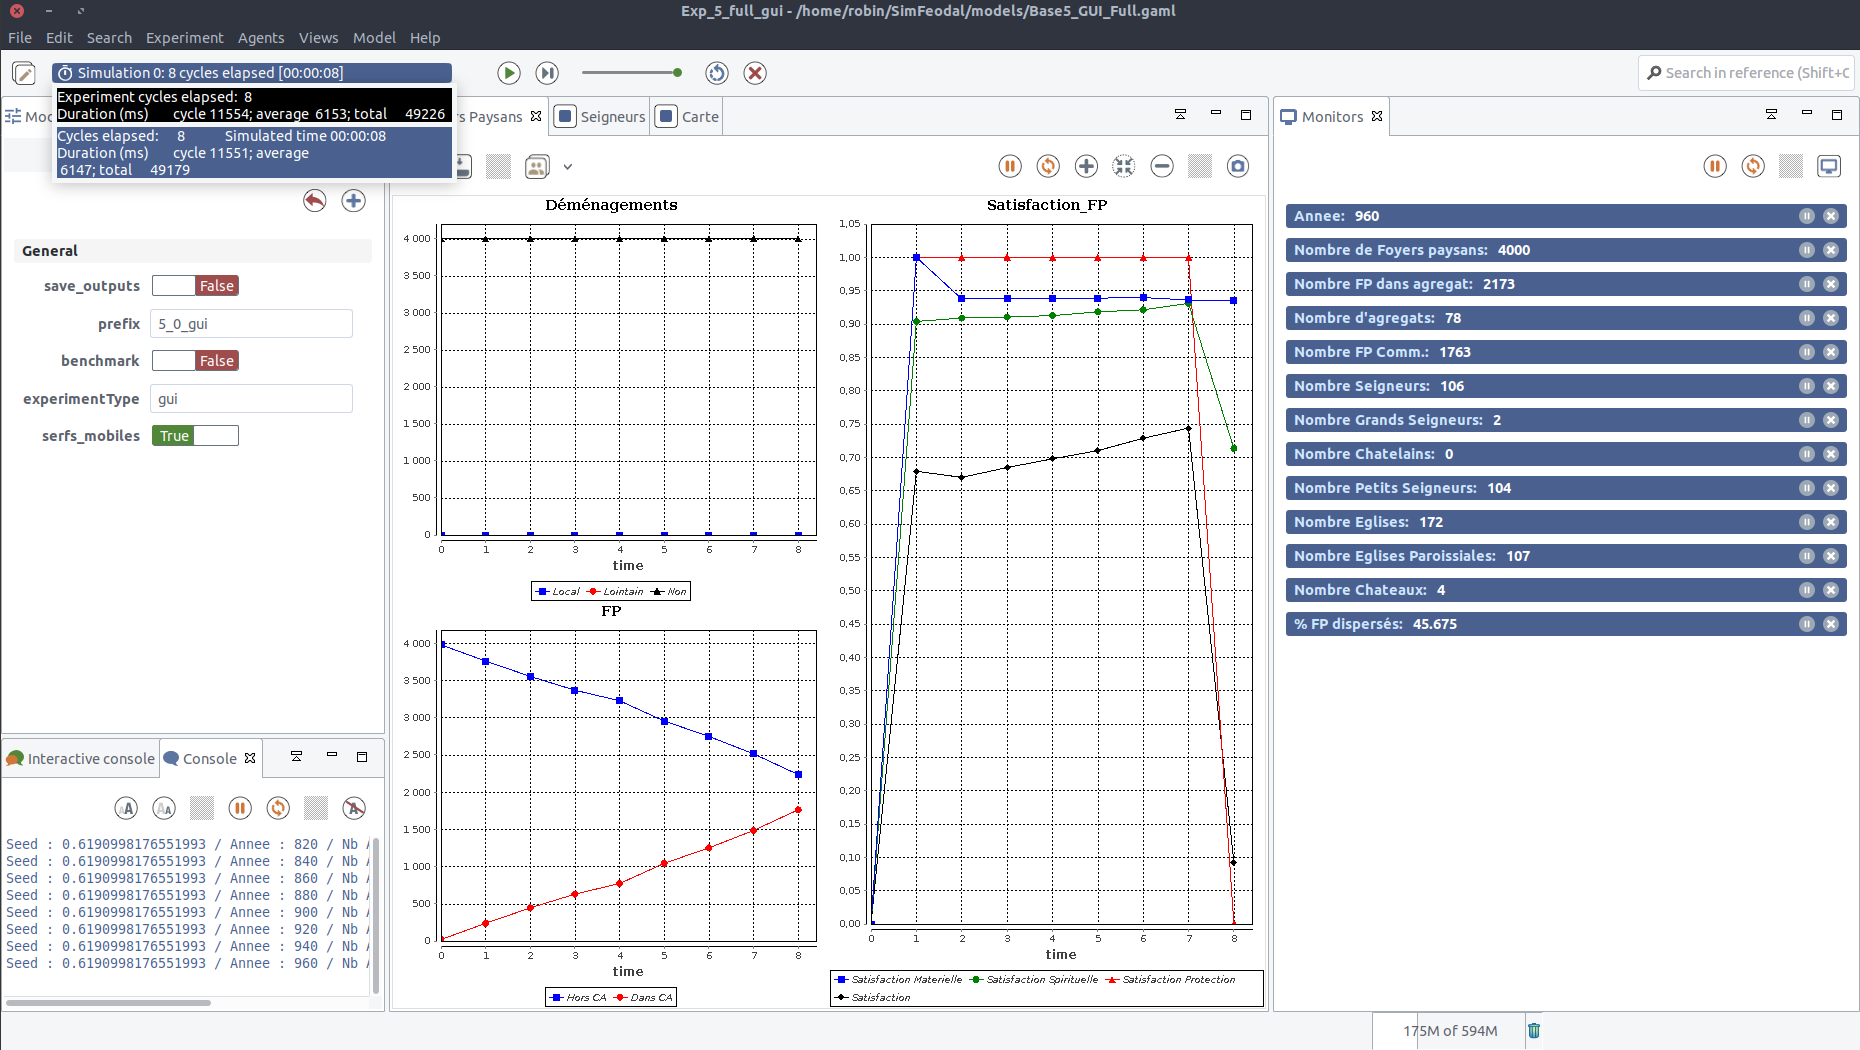
\includegraphics[width=\linewidth]{img/SimFeodal_GUI_FP.png}
		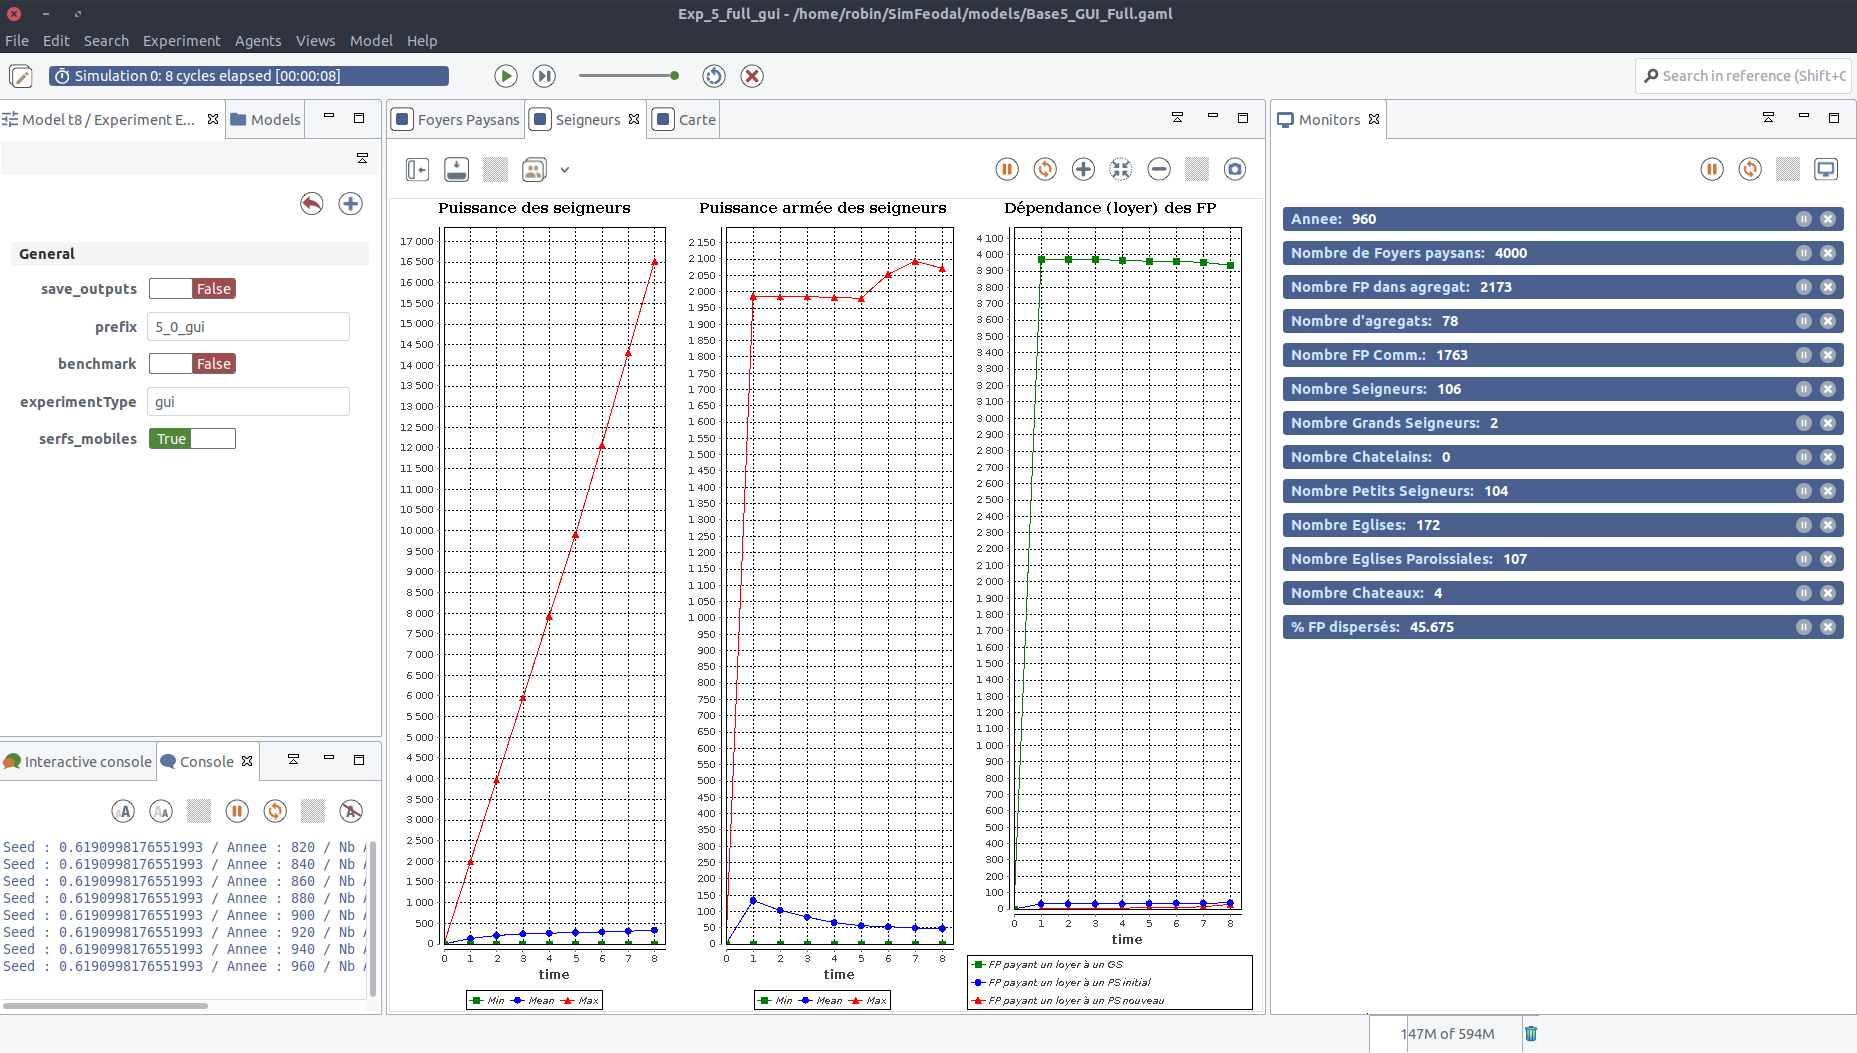
\includegraphics[width=\linewidth]{img/SimFeodal_GUI_seigneurs.png}
		\caption{Indicateurs intégrés à l'interface graphique interne de SimFeodal.
		Dans ces captures d'écrans, il s'agit d'indicateurs liés aux foyers paysans et aux seigneurs.}
		\label{fig:simfeodal_gui_indicateurs}
	\end{figure}
	
	La visualisation en direct n'est donc pas mobilisable en tant que méthode d'évaluation principale, mais elle peut tout de même, comme dans un usage très classique, être utilisée comme un outil de validation interne pour tester chaque modification dans les valeurs de paramètres, remplissant alors le rôle de \og préfiltre\fg{} décrit auparavant.
	Visualiser une seule simulation, avant d'en exécuter les réplications nécessaires, permet ainsi déjà de vérifier que les modifications apportées dans les valeurs de paramètre ou dans les mécanismes n'ont pas entraîné l'apparition de \textit{bugs} ou d'incohérences immédiatement visibles.

	Nous avons donc choisi de développer une interface graphique, très sommaire mais permettant des allers-retours rapides entre l'implémentation et l'exécution, au sein de l'implémentation de SimFeodal.
	Cette interface n'affiche qu'un nombre réduit d'indicateurs (\autoref{fig:simfeodal_gui_indicateurs}), ainsi qu'une représentation cartographique (\autoref{fig:simfeodal_gui_carte}) utile à une analyse rapide du comportement d'ensemble du modèle.

\begin{figure}[H]
	\captionsetup{width=\linewidth}
	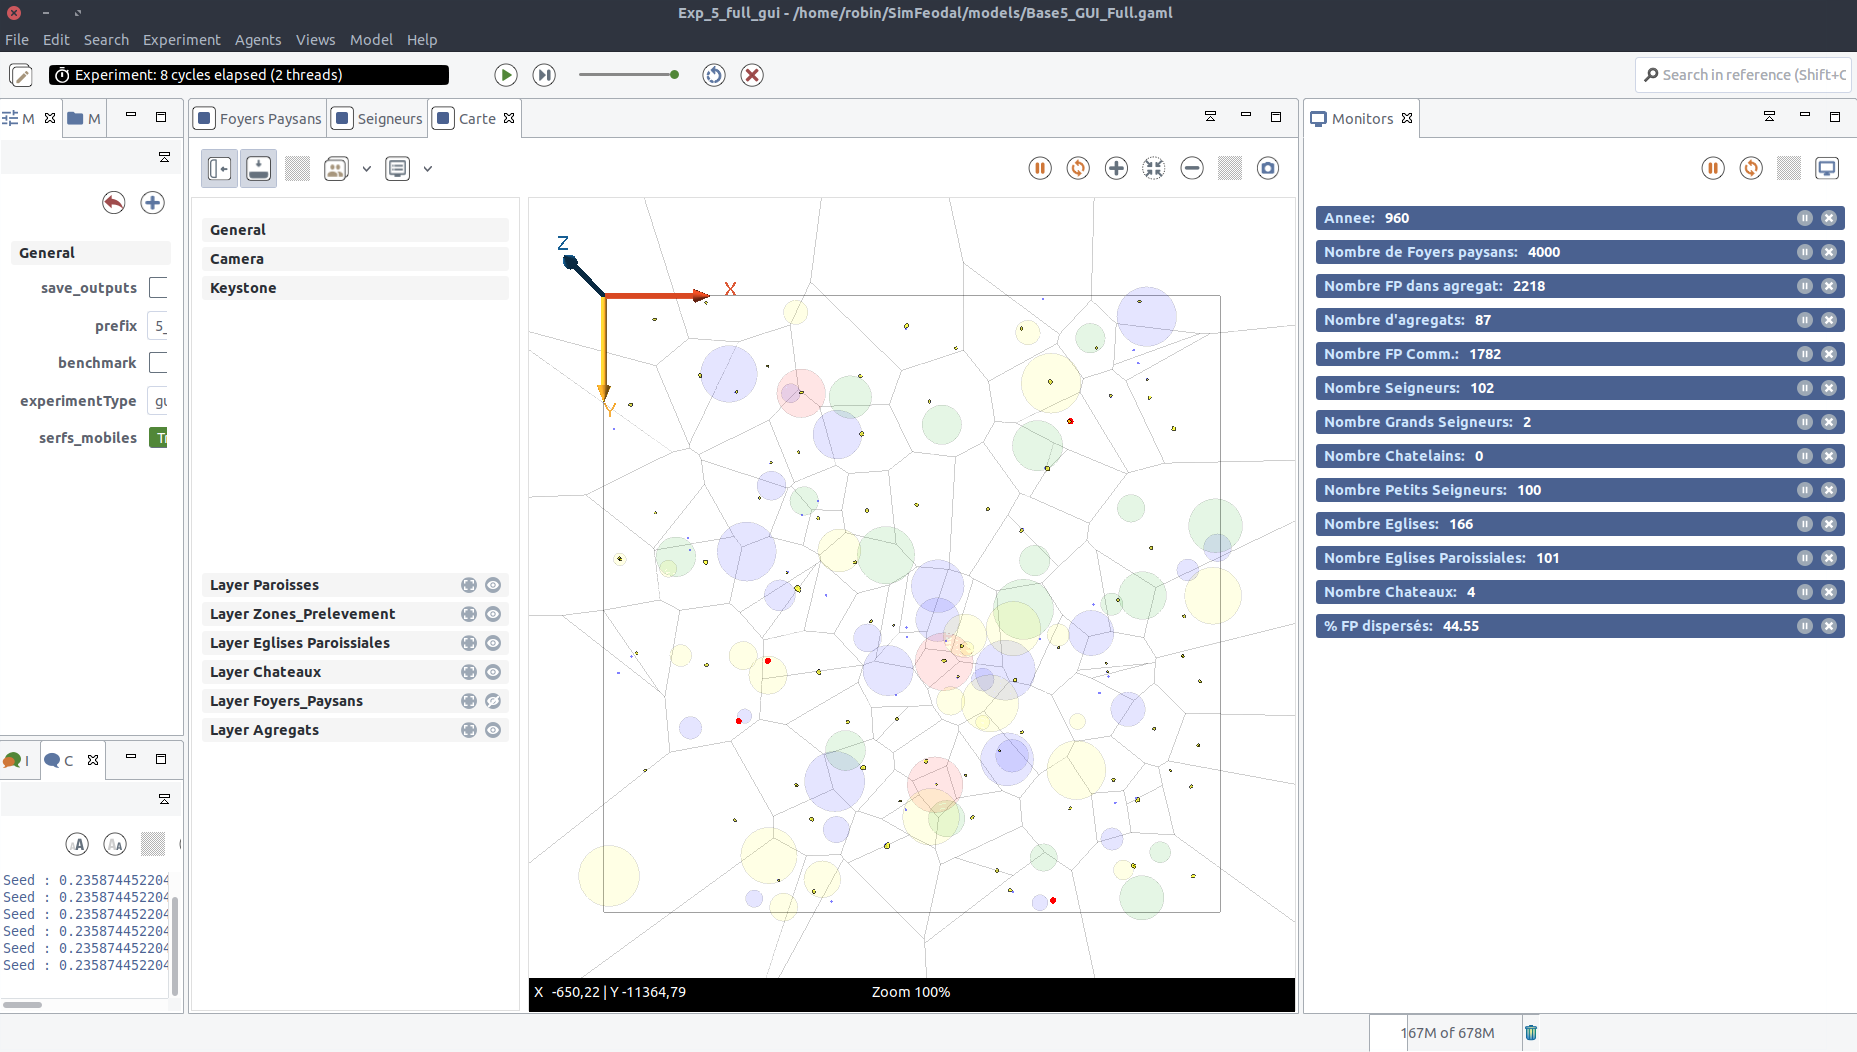
\includegraphics[width=\linewidth]{img/SimFeodal_GUI_carte.png}
	\caption{Visualisation intégrée à l'interface graphique interne de SimFeodal : cartographie synthétique de l'espace modélisé.}
	\label{fig:simfeodal_gui_carte}
\end{figure}

	Ces indicateurs intégrés à l'interface graphique interne de SimFeodal permettent de mener une étape préalable à l'évaluation du modèle.
	Cette étape vise à effectuer un premier filtrage des simulations avant d'exécuter les expériences en elles-mêmes.
	L'ajout de cette interface graphique vient donc renforcer l'outillage d'évaluation de SimFeodal.
	A cette étape, il manque encore un outil véritablement adapté à l'analyse conjointe des réplications du modèle, a posteriori de l'exécution des nombreuses réplications.

	\subsection{Générer les indicateurs}

	La production des indicateurs doit nécessairement être réalisée en aval de l'exécution des simulations (\og \textit{offline}\fg{} dans \cite{grignard_agent-based_2017}).
	Il faut pour cela disposer d'outils adaptés au traitement des données produites, c'est-à-dire répondant aux contraintes identifiées auparavant (\autoref{subsec:donnees-indicateurs}).
	La contrainte principale est d'être en mesure de gérer la masse de données produites.
	On l'a vu, cela élimine d'office les outils de type tableurs, ou encore les outils de manipulation graphique de données les plus courants.
	Pour les raisons évoquées dans le chapitre 1 (\hl{Positionnement : pourquoi utiliser des outils libres ?}), seules les solutions techniques libres étaient envisageables.

	Certains outils graphiques, basés sur des logiciels libres en arrière-plan (PSPP, R Commander, Orange), sont extrêmement aisés à prendre en main et auraient pu constituer un bon choix.
	Pourtant, avec une trentaine d'indicateurs à produire pour chaque expérience, donc de manière régulière, nous avons préféré nous tourner vers des outils plus orientés vers une interface en ligne de commande (\textit{Command Line Interface}, abrégés \textit{CLI}).

	L'utilisation de CLI a plusieurs intérêts gravitant autour de la reproductibilité des traitements.
	En premier lieu, ils permettent une adaptation aisée et rapide aux différents jeux de données.
	Ainsi, partant du principe que les données générées par les réplications et expérimentations sont de même structures, il suffit généralement de modifier le chemin d'entrée des fichiers résultants pour reproduire à l'identique une analyse sur un nouveau jeu de données.

	De manière plus technique, on peut remarquer que les différents indicateurs de sortie de simulation choisis présentent souvent des caractéristiques communes, aussi bien dans le traitement nécessaire que dans les formats (graphiques) produits.

	Par exemple, la grande majorité des indicateurs reposent sur une première agrégation des données par réplication et pas de temps simulé, puis par une seconde agrégation montrant la variabilité des situations générées, au niveau de l'expérimentation\footnote{
	On peut considérer ces agrégations comme une succession d'opération imbriquées : pour montrer l'évolution d'un indicateur tel que le taux de foyers paysans dispersés au cours du temps simulé, il faut (1) calculer le ratio entre nombre de foyers paysans dispersés et nombre total de foyers paysans, (2) pour chacun des pas de temps simulé, (3) pour chaque simulation, (4) pour l'ensemble des réplications d'une expérience, (5) éventuellement pour chacune des expériences d'une phase plus large d'expérimentation qui ferait varier des valeurs de paramètres.
	}.
	En terme de manipulation de données, seuls le calcul de la variable à mobiliser, et éventuellement l'agent caractérisé -- la variabilité du nombre de foyers paysans et la variabilité du nombre d'agrégats ne diffèrent que par le type d'agent sur lequel le calcul est effectué --, sont ainsi à adapter dans ces nombreux indicateurs de sortie.
	Les variations, en terme de code-sources, sont donc le plus souvent des adaptations minimes (nom de l'agent, type d'agrégation\ldots).
	Le recours à des traitements en \textit{CLI} permet ainsi un simple copier/coller, voir la création de fonctions dédiées, pour effectuer ces traitements très récurrents.

	Au niveau des sorties graphiques, on peut aussi remarquer que la structure des graphiques, en elle-même, est assez largement identique : on représente les pas des temps (les années simulées) en abscisse, un indicateur statistique en ordonnée, et la variabilité sous la forme de \textit{box-plot} minimalistes (\og \textit{minimal boxplot}\fg{}, promus par Edward Tufte pour minimiser le ratio données-encre \autocite[123-125]{tufte_visual_2001}).
	En disposant d'un environnement de type \textit{CLI}, et qui plus est en faisant usage de solutions graphiques construites sur une syntaxe régulière et générique (voir \cnameref{par:visualisation-pipeline}, \cpageref{par:visualisation-pipeline}), il devient très confortable de générer les différents indicateurs de sortie souhaités, puisqu'il suffit d'adapter les graphiques déjà conçus.

	Avec ces solutions logicielles d'analyse de données et de visualisation, il est facile de concevoir et d'implémenter les codes informatiques nécessaires à la génération des indicateurs de sortie de simulation.
	De plus, l'exécution de ces programmes est extrêmement rapide :  les différents fichiers de sortie de simulation sont lus et parcourus une unique fois pour en tirer toutes les variables nécessaires à l'établissement des indicateurs.

	\paragraph*{}
	En ayant choisi de mener une évaluation \textit{a posteriori} -- plutôt qu'en direct -- basée sur l'observation d'indicateurs générés -- par des outils adaptés au traitement de données massives -- de manière automatisée, on dispose donc, pour chaque expérience, d'un ensemble de fichiers numériques : chacun des indicateurs  de sortie est contenu dans un fichier unique, dans un format facilement exploitable et ré-utilisable. 

	\subsection{Organiser les indicateurs en rapports paramétrables}

	Du point de vue de la manipulation, la création de fichiers informatiques indépendants correspondant aux différents indicateurs de sortie de simulation est extrêmement pratique : on peut facilement les identifier, les transférer et les adapter, par exemple pour en rendre le contenu plus compréhensible par un public différent.

	En revanche, du point de vue de la comparaison des résultats, cette forme n'est pas la plus adaptée.
	Si l'on peut facilement comparer un même indicateur portant sur deux expériences différentes, la tâche se complique quand il s'agit d'avoir une vision globale des différences dans les indicateurs entre deux expériences.
	Pour cela, la démultiplication des fichiers correspondant aux indicateurs se révèle rapidement être un obstacle : l'utilisateur est en effet amené à jongler entre de très nombreux fichiers.
	
	\paragraph{Les rapports comme instruments de comparaison}
	Pour faciliter la comparaison d'indicateurs multiples -- et d'une forte diversité --, il est nécessaire de les organiser au sein d'une structure englobante.
	Nous entendons ici par organisation, une présentation structurée, suivant un certain ordre, identique selon les expériences, adaptée à une évaluation des résultats.
	Pour cela, nous avons choisi d'organiser les indicateurs de sortie de simulation au sein de \og rapports \fg{}.
	Cela permet, même en présence de nombreuses expériences, de rassembler l'ensemble des indicateurs de sortie propres à chacune dans un unique fichier, à la structure toujours similaire.
	Un premier apport, majeur, concerne l'archivage des sorties de simulation.
	Avec des rapports comprenant l'ensemble des indicateurs de sortie de chaque expérience d'un modèle, il est ainsi simple de conserver des traces de l'ensemble des versions et sous-version d'un modèle.
	Cela permet de garantir une certaine pérennité à ce modèle, à sa documentation, et ainsi simplifie le travail rétrospectif de caractérisation de l'évolution d'un modèle.	
	
	L'intérêt majeur de la structuration en rapports est surtout de faciliter la comparaison des expériences, c'est-à-dire des indicateurs de sortie des différentes expériences.
	On peut ainsi, par exemple, placer côte à côte, visuellement, deux rapports rendant compte de deux expériences différentes, et, en les faisant défiler simultanément, comparer point par point, c'est-à-dire indicateur par indicateur, leurs résultats respectifs, de manière visuelle et intuitive.

	Les formes que peuvent prendre des rapports, tout autant que les modalités de leur production, sont multiples et extrêmement diverses.
	La forme la plus simple et courante consiste à produire manuellement le rapport en insérant les indicateurs adaptés au fur et à mesure, par exemple dans un traitement de texte.
	A l'opposé, on peut noter les possibilités de créations entièrement automatisées de rapports complets, comprenant par exemple des descriptions et commentaires textuels générés à la volée, en fonction d'expressions conditionnelles\footnote{Voir par exemple l'application \og SOFIE\fg{} de l'Observatoire des Territoires du Commissariat général à l'égalité des territoires (CGET), qui génère automatiquement des commentaires relatifs aux inégalités femmes/hommes dans l'accès à l'emploi. Les commentaires propres aux types d'inégalités majeures de chaque EPCI sont produits de manière automatique depuis les données. \href{http://outils.observatoire-des-territoires.gouv.fr/sofie/}{http://outils.observatoire-des-territoires.gouv.fr/sofie/}
	}.

	Pour SimFeodal, nous avons choisi de restreindre au maximum la manipulation manuelle.
	On souhaitait générer un rapport entièrement automatique, ne requérant pas d'action spécifique en dehors du choix des données depuis lesquelles créer les indicateurs.
	A l'inverse, on a choisi de ne pas ajouter de fonctionnalité de commentaire automatique des indicateurs de sortie : la richesse -- et la difficulté-- d'une approche interdisciplinaire telle que la notre est constituée par la multiplication des analyses et points de vue.
	Il n'y avait donc aucun besoin de générer des commentaires standardisés et automatiques, forcément moins aboutis que les commentaires de chacun des co-concepteurs du modèle.
	Le rapport produit (\cref{fig:simfeodal_rapport_mini}) n'intègre donc que les indicateurs, sous forme de tableaux et de graphiques.
	Ces indicateurs sont organisés par partie, en l'occurrence en fonction du type d'entités et de comportement qu'ils décrivent.

	\begin{figure}[H]
		\captionsetup{width=\linewidth}
		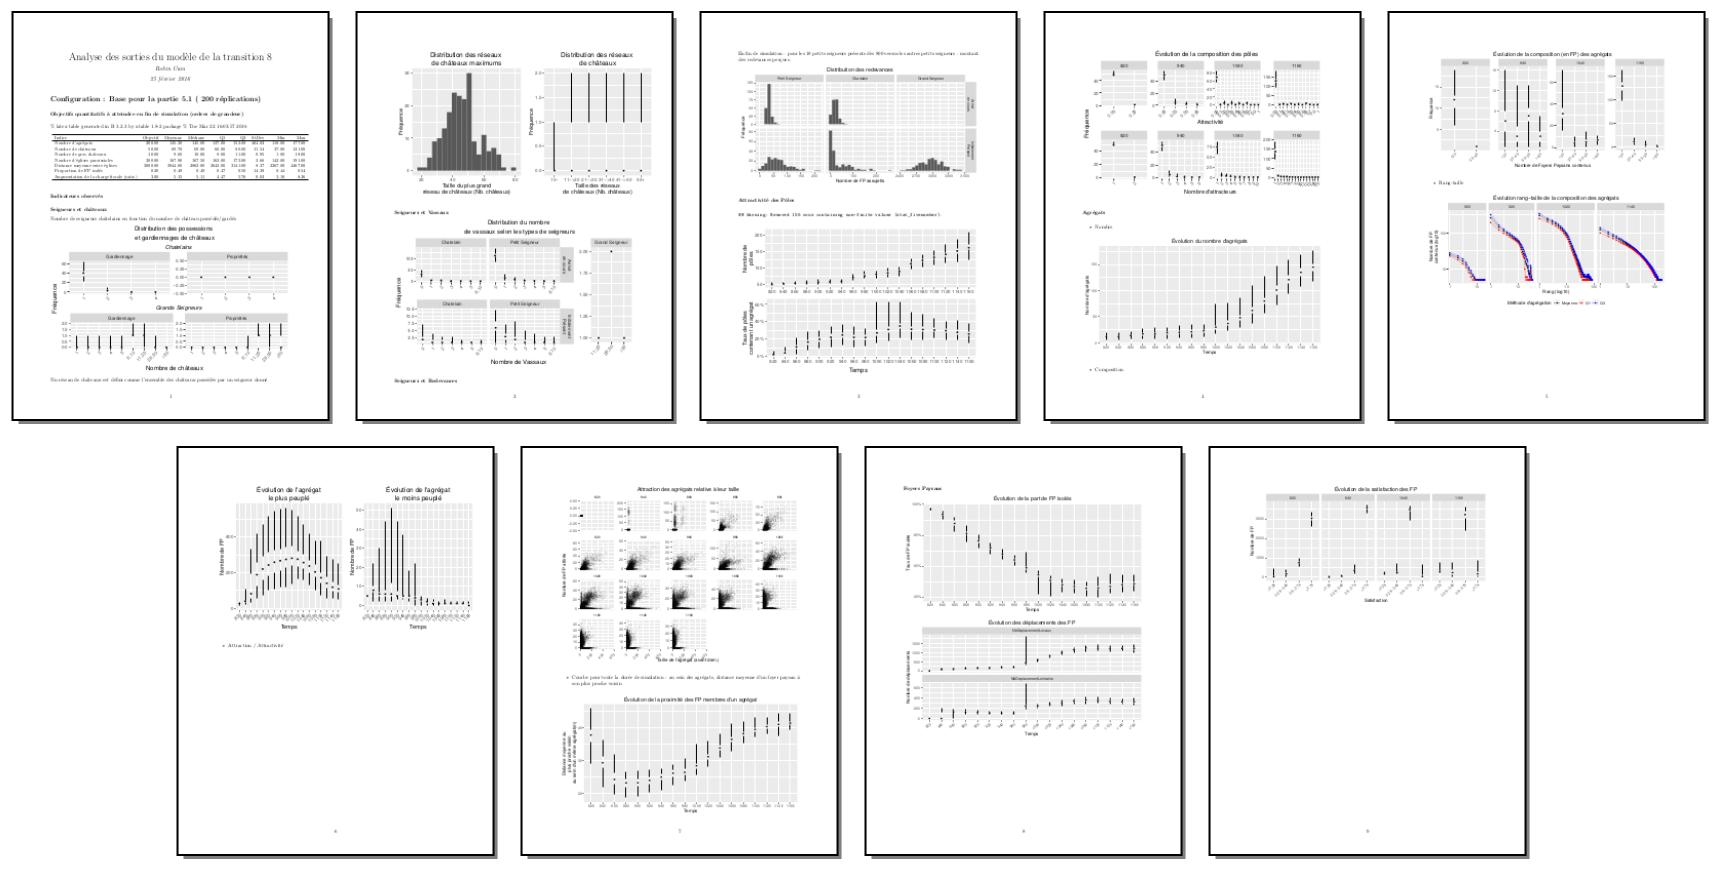
\includegraphics[width=\linewidth]{img/SimFeodal_Rapport_exemple.png}
		\caption{Un exemple de rapport automatique généré pour une expérimentation (étape 0) de SimFeodal. La version en taille réelle est reproduite en \hl{annexe X}.}
		\label{fig:simfeodal_rapport_mini}
	\end{figure}

\clearpage
	\paragraph{Structurer des rapports pour aller vers la reproductibilité des analyses}
	On a donc fait le choix de se baser sur des rapports automatisés et minimalistes, ne contenant que les indicateurs dans une forme structurée.
	Ce choix s'appuie sur des raisons multiples, qui ont toutes en commun une recherche de reproductibilité des résultats et des analyses menées.
	Une reproductibilité théorique (\hl{encore une ref au positionnement}), puisque les résultats de simulation doivent pouvoir être analysés et reproduits par des chercheurs potentiellement intéressés.
	Mais cette recherche de reproductibilité est aussi pratique, rendue aussi nécessaire par les méthodes de modélisation suivies.
	Tel qu'explicité auparavant (\cref{subsec:capter-replications,subsec:capter-experiences}), celles-ci s'appuient sur de nombreux allers-retours, ce qui requiert une capacité constante à reproduire et à affiner des résultats déjà observés.
	
	La quantité d'expériences requises pour arriver à un état satisfaisant du modèle est tributaire de ces allers-retours, et le nombre de rapports qu'il faut pouvoir produire est important.
	La fréquence de production de ces rapports est forte, et le modélisateur a alors tout intérêt à en fluidifier et accélérer le processus de création.
	
	Dans une telle situation, la création d'un rapport automatisé garantit une calcul et une production simplifié et rapide des indicateurs sur les nouvelles données.
	Cela permet un examen des sorties de simulation presque immédiatement après leur exécution.
	Cette automatisation permet aussi de mener une seconde évaluation -- après le pré-filtrage constitué par l'observation d'indicateurs en direct -- du bon déroulement \og interne \fg{}\footnote{
		Au sens de l'évaluation interne, c'est-à-dire du bon fonctionnement, exempt de \textit{bugs}, du modèle de simulation implémenté.
	}.
	Le caractère fixe d'un rapport automatisé se base ainsi sur une structure de données contraignante, par exemple constitués en \textit{n} fichiers dotés de plusieurs colonnes spécifiquement attendues.
	Les caractéristiques de ces données sont elles-mêmes contraignantes.
	Un rapport automatisé ne fonctionne, par exemple, qu'en présence d'un nombre pré-défini de réplications complètes.
	En l'absence d'un de ces critères dans des données en sortie de simulation, le rapport ne peut être généré et émet une erreur.
	Par exemple, si le nombre de réplications est plus faible qu'attendu, ou encore si tel attribut d'un agent a changé de type informatique, la création du rapport échoue.
	La présence ou non de cette erreur constitue donc un nouveau filtre de vérification de la validité du modèle.
	Cela permet, là encore, de détecter des simulations qui présenteraient des comportements incomplets ou aberrants en terme de production de données.

	Un autre intérêt majeur des rapports, déjà pointé en avantage des outils de type \textit{CLI} est leur adaptabilité.
	On a vu (\hl{chap. 3}) que les indicateurs à examiner sont nombreux et surtout, évolutifs, dans le sens où ces indicateurs ont fortement été modifiés, remplacés, affinés, au cours des étapes de paramétrage de SimFeodal.
	L'utilisation de rapports automatiques permet de minimiser le nombre de modifications à effectuer en cas de changements d'indicateurs.
	Le programme informatique qui génère les rapports s'appuie ainsi sur un code-source unique, générique aux simulations de chaque modèle.
	Lors d'un changement d'indicateurs, il suffit alors de modifier ce code-source en une seule place, et tous les appels à ce programme seront alors modifiés en conséquence.
	À partir de là, pour mettre à jour l'ensemble des rapports déjà produits, c'est-à-dire regroupant les indicateurs de chacune des expériences passées, il suffit de ré-exécuter la routine de production des rapports.
	
	Dans le cas de SimFeodal, caractérisé par de fréquents changements dans la forme et le calcul des indicateurs, cela a représenté un gain de temps et d'efficacité très conséquent.
	Par exemple, lors de certaines phases de paramétrage, on pouvait être amenés à faire évoluer le modèle quotidiennement et à tester, à cette même fréquence, plusieurs jeux de paramètres.
	Il fallait donc analyser les résultats de plusieurs expériences chaque jour, et régulièrement ajouter des indicateurs graphiques afin d'affiner l'évaluation.
	Ces indicateurs devaient aussi être ajoutés aux expériences des jours précédents, et au final, on re-générait parfois jusqu'à une plus d'une dizaine de rapports sur des cycles temporels courts de quelques jours.
		
	Par extension, cette même démarche d'automatisation, basée sur l'utilisation d'outils de type \textit{CLI}, devrait pouvoir s'appliquer à l'identique, avec les mêmes avantages, dans le cadre plus large de l'évaluation visuelle de modèles (\hl{ref chap 3, section 3.1.4}).

%	\begin{encadre}{Générer les rapports avec \texttt{R} et \texttt{knitr}}{technique-rapports-knitr}
%
%		\hl{Encadré sur les rapports automatiques, le \textit{\og litterate programming}\fg, le choix et le paramétrage de knitr + lien vers le code-source des rapports.}
%
%	\end{encadre}


	\paragraph{Dépasser les limites de la compatibilité d'ensemble}
	En réalité, la démarche de reproductibilité des rapports constitue plus un objectif théorique qu'un stade, \og reproductible\fg{} qu'il serait possible d'atteindre.
	Il s'agit ainsi plus de s'inscrire dans la voie de la reproductibilité que de chercher à parvenir à cet objectif largement inaccessible dans les faits.
	
	Comme explicité dans l'hl{encadré 3.2} sur l'incrémentalité des indicateurs, une limite forte empêche d'atteindre une reproductibilité absolue des analyses du comportement des différentes versions de SimFeodal.
	Les données générées par les différentes versions du modèle ne sont en effet pas systématiquement \og compatibles \fg{}.
	On entend par là qu'elles ne présentent pas toute exactement la même structure, à commencer par les variables enregistrées.
	Quand bien même il aurait été choisi dès le départ d'enregistrer le plus de sorties possibles, la reproductibilité de l'analyse échoue sur les données produites par le modèle et ses nombreuses versions : le modèle évolue, et avec lui, certaines variables apparaissent et d'autres deviennent caduques.
	La structure contraignante et précise des données nécessaires à la génération des rapports ne peut être entièrement satisfaite.
	La prise en compte de l'évolution du modèle demande une adaptation régulière -- mais aussi rare que possible -- des programmes qui génèrent ces rapports.
	
	On ne peut donc satisfaire globalement à un objectif de reproductibilité, mais il est toutefois possible de limiter la déviance à cette ambition.
	Pour cela, on peut agencer les différentes versions du modèles au sein de \og générations\fg{} de modèle, c'est-à-dire d'ensembles de versions présentant des attributs comparables et générant des données de même structure.
	Plutôt que d'adapter le code-source des rapports à chaque nouvelle version du modèle, ou encore de ne jamais l'adapter et donc d'être tributaire de la structure des toutes premières versions du modèle, cela constitue un choix intermédiaire qui permet de limiter le nombre de variantes de rapports.
	Cette approche suit les grandes lignes du développement logiciel général. Les itérations successives d'un logiciel sont constituées de versions \og majeures\fg{} -- les générations de modèles dans notre cas --, qui n'assurent pas nécessairement de compatibilité avec les versions majeures précédentes, et de versions \og mineures\fg{}, dans lesquelles la compatibilité est assurée\footnote{
		Par exemple, un fichier de dessin vectoriel créé avec le logiciel Adobe Illustrator 15.0 ne sera pas lu correctement avec une version 14.0.
		Ce fichier présentera toutefois un compatibilité parfaite avec les versions 15.1 à 15.\textit{n} du logiciel.
	}.
	
	Pour revenir aux rapports voués à l'évaluation d'un modèle, en inscrivant les différentes versions du modèle -- et des programmes générant les rapport correspondant -- dans des sous-ensemble de versions, les \og générations\fg{}, les différents rapports peuvent être considérés comme reproductibles et automatiques au sein de ces générations.
	Pour SimFeodal, cela implique d'organiser les différentes versions du modèle -- résultant des étapes de paramétrage, \hl{cf. chap4} -- au sein de grandes générations, à chaque changements structurels des mécanismes ou données produites par le modèle.
	
	\hl{Ajouter un schéma avec les générations, versions et sous-versions}
	
	\paragraph{Les rapports, des instruments suffisants ?}
	
	A l'issue de la conception et de l'implémentation de ces rapports automatiques, on dispose donc, pour chaque expérience, d'un document aisément partageable et lisible.
	Ces documents s'enrichissent, au fur et à mesure des générations de modèles, de nouveaux indicateurs, et sont comparables au sein de ces générations.
	Cela pourrait constituer la dernière étape de la création d'outils d'évaluation d'un modèle, dans la limite d'un nombre de versions ou de génération de modèles assez restreint.
	
	SimFeodal, comme c'est souvent le cas dans les modèles à base d'agent, a toutefois été caractérisé par une forte quantité d'allers-retours entre le modèle et ses résultats, entraînant à chaque fois de nouvelles expérimentations (cf. \cref{sec:sorties-simfeodal}). 
	
	On a vu que la manipulation d'un grand nombre d'indicateurs, même pour une quantité restreinte d'expériences, disqualifiait l'usage de fichiers individuels et poussait à l'usage de rapports structurés.
	Avec un grand nombre d'expériences, les mêmes limites apparaissent pour les rapports : la masse d'expériences rend partiellement caduque l'utilisation unique des rapports automatiques.
	Il est en effet aisé de comparer, sur un même écran d'ordinateur, deux ou trois rapports, mais dès lors qu'il faut en comparer un plus grand nombre, la manipulation conjointe des rapports devient complexe, tout autant que d'avoir une vision globale des résultats principaux de chaque expérience.

\clearpage
	\subsection{Organiser les rapports : Dashboards}\label{subsec:dashboards}

	Pour être en mesure de comparer de nombreux éléments, il est nécessaire de passer d'une exploration linéaire, fondée sur le visualisation successive de chacun des indicateurs, à une exploration globale et interactive.
	En pratique, plutôt que de faire défiler visuellement les nombreuses pages d'indicateurs, mieux vaut une interface présentant les points clefs de l'évaluation et qui permette d'entrer dans le détail de chacun des indicateurs dans un second temps, sur demande.
	Comme le résume le \og mantra\fg{} de l'analyse visuelle (\og \textit{Visual information-seeking mantra}\fg{}) de \citeauteur{shneiderman1996eyes} :
\begin{quote}
	\centering
	\noindent\og Overview first, zoom and filter, then details on demand\fg{}\\
	\mbox{}~ \hfill \cite[\ppno~2]{shneiderman1996eyes}
\end{quote}
	

	\subsubsection{Les \textit{dashboards}}

	Cette logique, assez universelle désormais, est celle qui préside à la création des nombreux \og tableaux de bord \fg{}, ou \og \textit{dashboards} \fg{} que l'ont voit émerger depuis la fin des années 1990.
	Rob Kitchin et ses co-auteurs définissent ainsi les \textit{dashboards}, en s'appuyant sur les travaux de Few notamment :

	\begin{quotation}
		\og For Few [\autocite[p.34]{few_information_2006}] a ‘dashboard is
		a visual display of the most important information needed to achieve one or more objectives; consolidated and arranged on a single screen so the information can be monitored at a glance’.
		Just as a car dashboard provides critical information needed to operate the vehicle at a glance, indicator dashboards provide key information for running companies or cities (\st{Dubriwny \& Rivard, 2004})[\autocite{rivard_are_2004}].\fg{}\\
		\mbox{}~ \hfill \cite[p. 11]{kitchin_knowing_2015}
	\end{quotation}

	Très répandus dans le monde de l'informatique décisionnelle (\textit{Business Intelligence, BI}), ces outils permettent d'explorer des données d'entreprises, par exemple des résultats financiers.
	Pour ce faire, ils mettent en avant, dans une interface unique, des indicateurs clés (\textit{Key Performance Indicators, KPI}), qu'il est ensuite possible de filtrer et d'affiner, par exemple par sélection de différents intervalles temporels.

	Les \textit{KPI} jouent le rôle d'indicateurs synthétiques, c'est-à-dire qu'ils s'adressent à des gestionnaires, par exemple des \textit{managers}, qui ont une expertise importante sur les résultats produits.
	Les utilisateurs des \textit{dashboards} ne sont donc pas des analystes, à même d'explorer eux-mêmes les données mobilisées, mais plutôt des thématiciens qui se fondent sur les indicateurs présentés pour prendre des décisions.

	La dichotomie \og analyste/décisionnaire\fg{} s'exprime aussi dans le domaine de la recherche, et notamment dans la recherche en géographie urbaine à visée applicative.
	Avec l'avènement des données massives et de leur prise en compte pour la gestion des villes (\textit{smart cities}), les géographes se sont aussi penchés sur des outils de ce type.
	En résulte une utilisation de plus en plus fréquente de \textit{dashboards} en géographie urbaine (\og \textit{city-dashboards}\fg{}, \cite{roumpani_creating_2013, kitchin_knowing_2015, batty_perspective_2015}).

	Le parallèle avec le monde de l'informatique décisionnelle est en effet présent dans les types d'utilisateurs et de producteurs de ces outils.
	Il s'agit de mettre à disposition d'experts thématiques (les décideurs publiques) des indicateurs clés, issus de calculs parfois complexes.
	Cela afin de leur permettre d'évaluer une situation donnée et de prendre les décisions politiques adéquates.

	Le constat ayant mené à l'apparition des premiers \textit{dashboards}, tant en informatique décisionnelle qu'en géographie urbaine, est identique.
	Les informations nécessaires à l'évaluation d'une situation (financière, relative aux politiques publiques\ldots) sont de plus en plus nombreuses et hétérogènes.
	Les indicateurs permettant de mener ces évaluations, pensés pour les décideurs qui en feront usage (\textit{managers}, acteurs publiques\ldots), se démultiplient et se diversifient aussi par conséquence.

	Inspiré autant par l'usage \textit{BI} que par l'usage géographique, nous considérons que ces outils peuvent se révéler utiles dans l'évaluation de modèles de simulations complexes.
	Les enjeux sont en effet les mêmes : permettre à des thématiciens de comprendre et d'évaluer les sorties d'un modèle, à l'aide d'indicateurs nombreux et complexes présentés de manière transparente relativement à cette complexité.

	Ce positionnement méthodologique s'inscrit pleinement dans la démarche de co-construction interdisciplinaire de SimFeodal.
	On y retrouve ainsi la même logique qui anime les dashboards : une évaluation menée par des thématiciens qui s'appuient pour cela sur des indicateurs clefs (\hl{ref. aux indicateurs les plus importants dans le chap 3}) et précisent leur analyse à l'aide d'indicateurs secondaires présentés sous forme d'un panel varié de visualisations.
	Nous avons donc choisi de ré-organiser les rapports initialement produits pour leur donner une forme plus adaptée à ces enjeux, sous forme de \textit{dashboards}.

	\subsubsection{SimVADB}\label{subsubsec:simvadb}

	Les \textit{dashboards} font souvent usages de représentations graphiques très métaphoriques des tableaux de bords automobiles.
	On y retrouve fréquemment une forte mise en valeur d'indicateurs numériques simples au travers de représentations \og skeuomorphes\fg{}, c'est-à-dire qui reprennent l'apparence physique des objets symbolisés.
	On retrouve communément, par exemple, des indicateurs représentés sous forme de jauges (\textit{gauge charts}), de thermomètres (\textit{thermometer charts}), ou encore de voyants d'alerte et autres témoins lumineux (\cref{fig:skeuomorphism})).
	
	\begin{figure}[H]
		\centering
		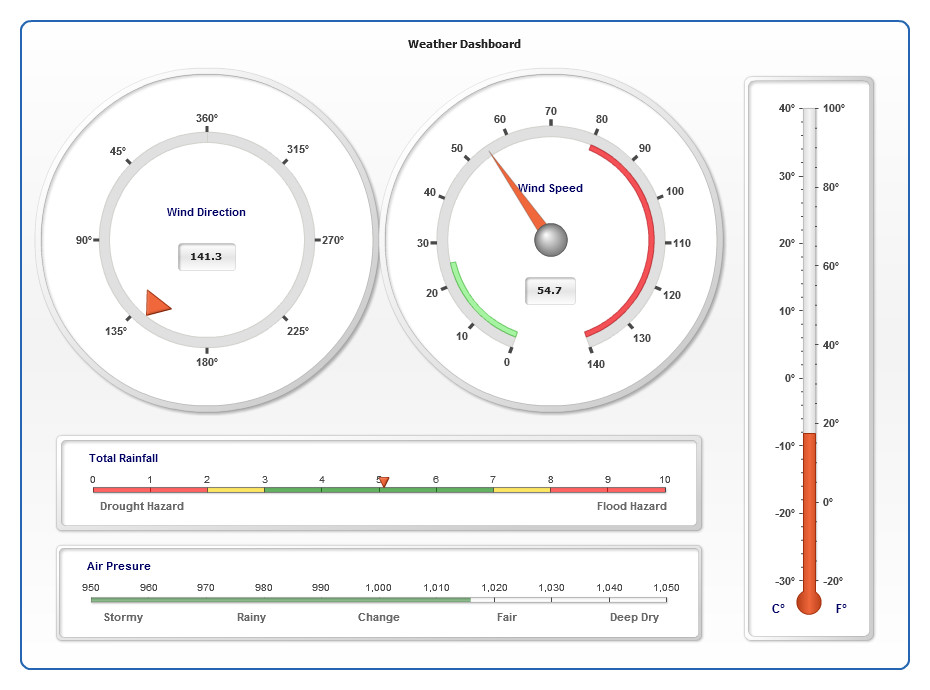
\includegraphics[width=.8\linewidth]{img/skeuomorphism.jpg}
		\caption{Un exemple de représentations visuelles courantes dans les \textit{dashboards}. Tiré de \textcite{pandre_charts_2011}}
		\label{fig:skeuomorphism}
	\end{figure}
	
	
	Pour SimFeodal, les indicateurs étant assez fortement conçus et structurés (\hl{chap. 3}), nous n'avons pas ressenti le besoin de faire appel à ce type de représentation.
	Nous avons donc emprunté aux \textit{dashboards} la logique d'organisation visuelle des indicateurs plutôt que les modes de visualisation en eux-mêmes.
	Pour faciliter la transition pour l'utilisateur, on cherchait ainsi à produire un \textit{dashboard} au plus proche, visuellement, des rapports automatiques qui les précédaient.

	On a pour cela développé un \textit{dashboard} adapté à SimFeodal, nommé SimVADB\footnote{
	\textbf{S}imulation \textbf{V}isual \textbf{A}nalysis \textbf{D}ash\textbf{B}oard.\\
	Cette application a rapidement été remplacée par l'itération suivante (SimEDB, voir \cref{subsec:explo-interactive}), et n'a donc dans les faits jamais été complètement finalisée. On en trouve une trace, fonctionnelle mais incomplète (les versions ultérieures n'ont pas été enregistrées dans l'outil de versionnement), dans ce dépôt logiciel :
	\href{https://github.com/RCura/SimEDB/tree/2cd22c7ccfbcf31f4a09550c2396932c46ef2622}{https://github.com/RCura/SimEDB/tree/2cd22c7c}
	}.
	Dans un premier temps, on souhaitait simplement ré-organiser le code-source produisant les rapports automatiques, afin de convertir ces rapports en \textit{dashboards}.
	Cela a été effectué au moyen d'outils permettant de générer des applications en ligne, sans changer de langage de programmation.
	Dans ce cas, on s'est appuyé sur la librairie logicielle \textsf{Flexdashboard} \autocite{iannone_flexdashboard_2018}.
	
	Le passage du rapport automatique au \textit{dashboard} illustre l'un des grands intérêts des outils de type \textit{CLI} : dans le cas de SimVADB, il a suffit de ré-organiser le code, sans modifier à aucun moment les fonctions de calcul et de création des indicateurs de sortie de simulation.
	Les codes \ref{lst:code-rapport} et \ref{lst:code-dashboard} illustrent la facilité de cette modification.
	Il s'agit véritablement de placer les différentes fonctions dans des blocs graphiques.
	Ces modifications minimes augmentent toutefois considérablement la convivialité et la facilité de l'analyse de résultats de sortie d'un modèle.
\clearpage

\lstset{frame=shadowbox, tabsize=2}
\noindent\begin{minipage}[t]{.44\textwidth}
{\footnotesize
	\begin{lstlisting}[caption={Pseudo-code du rapport automatique.},frame=tlrb, captionpos=b, label = {lst:code-rapport}]
# Agent de type A
	afficher('Agent de type A')
	
	print('Indicateur 1')
	calcul_indicateur_1 {...}
	affichage_indicateur_1 {...}
	
	afficher('Indicateur 2')
	calcul_indicateur_2 {...}
	affichage_indicateur_2 {...}
# Agent de type B
	afficher('Agent de type B')
	[...]
	\end{lstlisting}
}
\end{minipage}\hfill
\begin{minipage}[t]{.53\textwidth}
{\footnotesize
	\begin{lstlisting}[caption={Pseudo-code du dashboard.},frame=tlrb, captionpos=b, label = {lst:code-dashboard}]
onglet{titre = 'Agent de type A',
	sous_onglet{titre = 'Indicateur 1',
		calcul_indicateur_1 {...}
		affichage_indicateur_1 {...}
	},
	sous_onglet{titre = 'Indicateur 2',
		calcul_indicateur_2 {...}
		affichage_indicateur_2 {...}
	}
},
onglet{titre = 'Agent de type B',
	[...]
}
	\end{lstlisting}
}
\end{minipage}
	
	Comme dans l'exemple de code, on a préféré organiser les indicateurs au seins d'onglets plutôt que de les présenter dans des pages successives.
	Les onglets de premier niveau représentaient les types d'agent, et des onglets de second niveau permettaient de visualiser l'ensemble des indicateurs associés à ces agents (\cref{fig:mockup_simvadb}).

\begin{figure}[H]
	\centering
	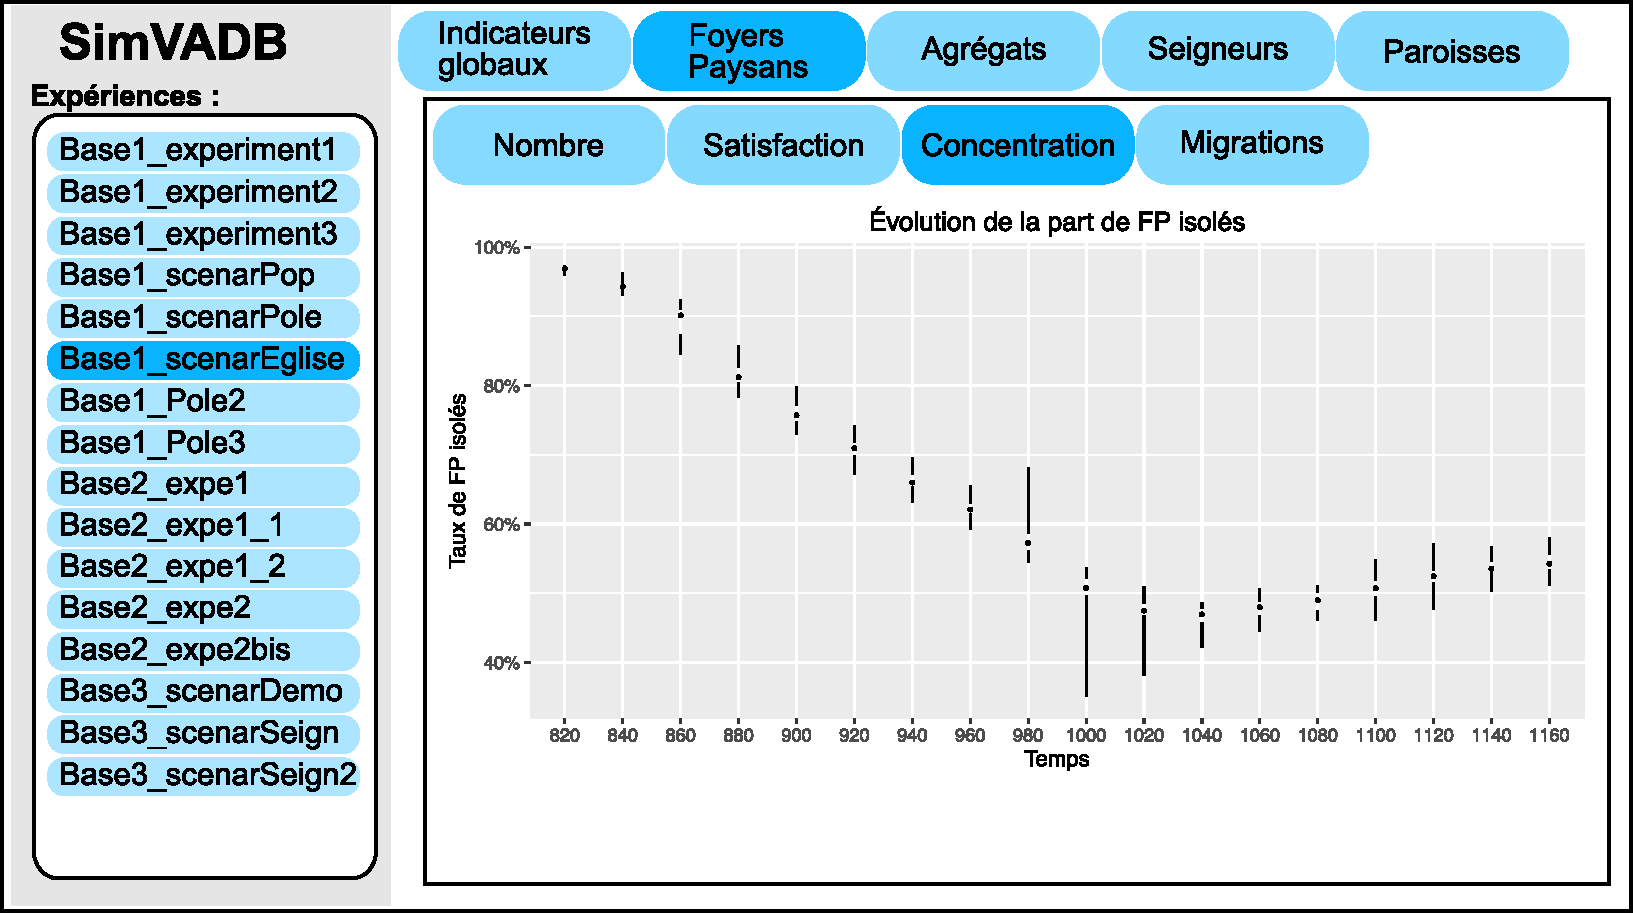
\includegraphics[width=\linewidth]{img/simvadb_mockup.pdf}
	\caption{Un \textit{mock-up} de la première interface de SimVADB, un \textit{dashboard} dédié à la visualisation des indicateurs de sorties de simulation de SimFeodal.}
	\label{fig:mockup_simvadb}
\end{figure}

	Au niveau de l'interface utilisateur, SimVADB permettait de choisir, via un menu de sélection (partie de gauche dans la \cref{fig:mockup_simvadb}), les expériences passées dont on voulait visualiser les indicateurs de sortie (les deux niveaux d'onglets de la partie de droite).

	
	\paragraph{Les limites du \textit{dashboard}}
	Avec la multiplication des valeurs de paramètres testées, il est devenu plus efficace de regrouper les expériences au sein d'expérimentations.
	Celles-ci voient varier plusieurs paramètres, potentiellement avec de multiples valeurs de paramètres pour chacun.
	Elles constituent donc un ensemble d'expériences qui partagent des mécanismes et un jeu de paramètre par défaut communs.

	Avec le mode de sélection choisi dans SimVADB, basé sur le nom des expériences, il devenait plus difficile de sélectionner rapidement des ensembles d'expériences membres d'une même phase d'expérimentation.
	En effet, et comme illustré dans la \cref{fig:mockup_simvadb}, les noms d'expériences tendent à s'allonger, et avec leur masse augmentant, il est peu commode d'avoir à parcourir tout un long menu de sélection pour trouver les expériences souhaitées.
	De plus, malgré des tentatives de nommage régulières et explicites, la multiplication des expériences et expérimentations implique aussi une certaine confusion dans les types de mécanismes et valeurs de paramètres associés.
	Sans table de correspondance complète entre les noms des expériences et leurs valeurs de paramètres, il devenait impraticable de retrouver les différentes expériences mettant en avant, par exemple, des attractivités fortes par les pôles, une plus forte hiérarchisation des attracteurs ou encore des migrations lointaines facilitées.
	Le choix méthodologique d'interaction avec la plate-forme d'affichage des indicateurs, basé sur une sélection des expériences depuis leur nom, s'est donc révélé inadapté à la sélection et à l'exploration des sorties de SimFeodal.
	
	
	Au delà du soucis du mode d'interaction, qui aurait pu être amélioré, un autre problème apparaissait.
	Pour évaluer visuellement différentes configurations du modèle, on ne pouvait se contenter d'un simple affichage des données, au sein d'un outil de type présentoir interactif tel que SimVADB.
	Comme dit dans \hl{le chapitre 4}, le paramétrage de SimFeodal a ainsi reposé sur de nombreuses étapes d'évaluation des différentes version du modèle.
	L'approche d'analyse principale était donc la comparaison, point par point, entre les résultats des indicateurs de sortie de simulation des versions successives de SimFeodal.
	Un outil de présentation dynamique de résultats de sorties de simulations est certes plus adapté qu'un rapport statique, mais il ne constitue pas pour autant un outil adapté à la comparaison.
	S'il suffit pour de la restitution, par exemple dans le cadre du rapport systématique des résultats de SimFeodal, on ne peut s'appuyer uniquement sur une succession d'évaluations visuelles pour appréhender l'étendue des changements apportées par une modification des valeurs de paramètres.

	\subsection{Interagir avec les rapports : exploration interactive}\label{subsec:explo-interactive}

	Face à la démultiplication des expérimentations, consécutive aux nombreuses étapes de paramétrage de SimFeodal (\hl{cf. chap 4}), il a fallu repenser la plate-forme d'évaluation des résultats.
	Pour cela, considérant que les simulations ne pouvaient être aisément appréhendées et sélectionnées par leur nom, numéro d'étape ou de version, il a été décidé d'adopter une posture plus proche de l'exploration du modèle en elle-même.
	C'est-à-dire de ne pas caractériser les simulations par un identifiant quelconque, mais plutôt par leur spécificité intrinsèque, c'est-à-dire la combinaison de valeurs de paramètres qui les rendent uniques.
	Ce faisant, au sein de la plate-forme d'exploration SimVADB, l'enjeu devenait plutôt la compréhension des effets des valeurs de paramètres sur les indicateurs que l'évaluation d'une simulation en particulier.
	Il fallait passer du descriptif, quelle qu'en soit la méthode, à du comparatif.
	
	Du point de vue de l'interface utilisateur, cela implique que la sélection ne se fasse plus par un unique critère (le nom de la simulation), mais au contraire sur du multi-critère.
	Par une succession de sélections, chaque paramètre pouvait constituer un nouveau filtre dans lequel on avait à choisir les valeurs à interroger (voir la \cref{fig:schema_parcoords} \textbf{(E)} de l'\cref{enc:parcoords}).

	La quantité de paramètres en entrée était importante et pouvait dès lors donner lieu à un mode de sélection complexe et fastidieux -- définir une par une les valeurs voulues pour chacun des 45 paramètres --.
	Nous avons choisi encore une fois de nous appuyer sur l'aspect visuel afin de permettre aux utilisateurs de SimVADB de choisir la ou les expérimentations à analyser.
	
	
	\paragraph{Visualiser avec des coordonnées parallèles }

	Pour cela, on a choisi de représenter les combinaisons de paramètres dans un graphique en \og coordonnées parallèles \fg{} (\textit{parallel coordinates}, d'après \cite{inselberg_parallel_1987}, voir \cite{few_multivariate_2006} par exemple pour une description plus succincte, illustrée et pratique).
	Ce type de graphique est en effet extrêmement pertinent pour représenter une information multi-dimensionnelle en ce qu'il permet de détecter graphiquement des \textit{clusters} d'individus statistiques\footnote{
		Ici, chaque expérience est un individu statistique.
		Il est caractérisé par un ensemble de variables, les différents paramètres, et les modalités de ces variables que cet individu emprunte (les valeurs de paramètres).
		Quand le nombre d'individus est important, les différentes \og courbes\fg{}, qui correspondent au profil des individus sur le graphique en coordonnées parallèles, peuvent se superposer et montrer des tendances similaires.
		Avec ce type de représentation, il est facile de visualiser les grandes classes d'individus constituées par ces \og tendances\fg{}, et donc de constater des distinctions entre les individus (les expériences) de manière visuelle.
	} \autocite[2]{heinrich_state_2013}, c'est-à-dire de faire ressortir visuellement les expériences dont les valeurs de paramètre sont proches.
	Notons bien que l'on parle ici des valeurs de paramètres, c'est-à-dire des conditions des expériences, et non des indicateurs de sortie.
	L'approche va ainsi des paramètres aux résultats : depuis des valeurs de paramètres choisies, on analyse la diversité des résultats.
%	L'approche inverse, souvent menée en simulation agent (\hl{ref à chap 3, exploration automatique}}), pourrait mener une classification des résultats de sortie pour reporter cette classification sur les valeurs de paramètres.

	
	\paragraph{Interagir avec des coordonnées parallèles}
	De plus, en matière d'interaction, on utilise fréquemment les graphiques en coordonnées parallèles en vue de filtrage.
	Cette opération est le plus souvent menée par des actions de \textit{brushing} (\og brossage\fg{}), c'est-à-dire de sélection graphique d'une zone en dessinant son étendue à la souris (voir \cref{enc:parcoords}).
	Ce type de sélection se révèle en effet souvent plus efficace et intuitive qu'une sélection textuelle plus systématique :
	
	\begin{quotation}\vspace{-0.5cm}
		\og Filtering is an operation that removes signals from its input. A filter reduces the number of lines to be rendered. In this sense, dynamic querying [...] is a filter, if implemented with brushing [...], which reduces clutter by putting the filtered lines in focus using some highlighting mechanism. Combining simple brushes using logical operators [...] further allows the user to formulate rather complex queries that might even achieve faster and more accurate results using parallel coordinates than using a Structured Query Language (SQL) [...].\fg{}\\
		\mbox{}~ \hfill \cite[p. 13]{heinrich_state_2013}
	\end{quotation}
	
	\begin{encadre}{Construction et utilisation interactive d'un graphique en coordonnées parallèles}{parcoords}

	La \cref{fig:schema_parcoords} illustre les étapes successives de construction d'un graphique en coordonnées parallèles, depuis le tableau statistique (\textbf{A}) jusqu'au graphique final (\textbf{D}).
	
	Pour cela, on projette les valeurs des variables sur des axes représentant chacune des variables (\textbf{B}).
	En normalisant la taille de ces axes et en les plaçant en parallèle (\textbf{C}), on peut alors tracer les \og profils\fg{} des variables en reliant les positions de chacun des individus statistiques sur chacun des axes (\textbf{D}).
	
	La seconde partie de la figure représente le mode d'interaction par \textit{brushing} : on \og brosse\fg{} sur chaque axe une sélection de valeurs à conserver (\textbf{E}).
	La sélection graphique est convertie en intervalles numériques et formalisée sous une forme classique (\textbf{F}) qui permet de filtrer les données sous-jacentes.
	Au final, cette opération renvoie le seul individu statistique répondant aux deux sélections graphiques (\textbf{G}).
	
	\begin{figure}[H]
	\centering
	\captionsetup{width=\linewidth}
	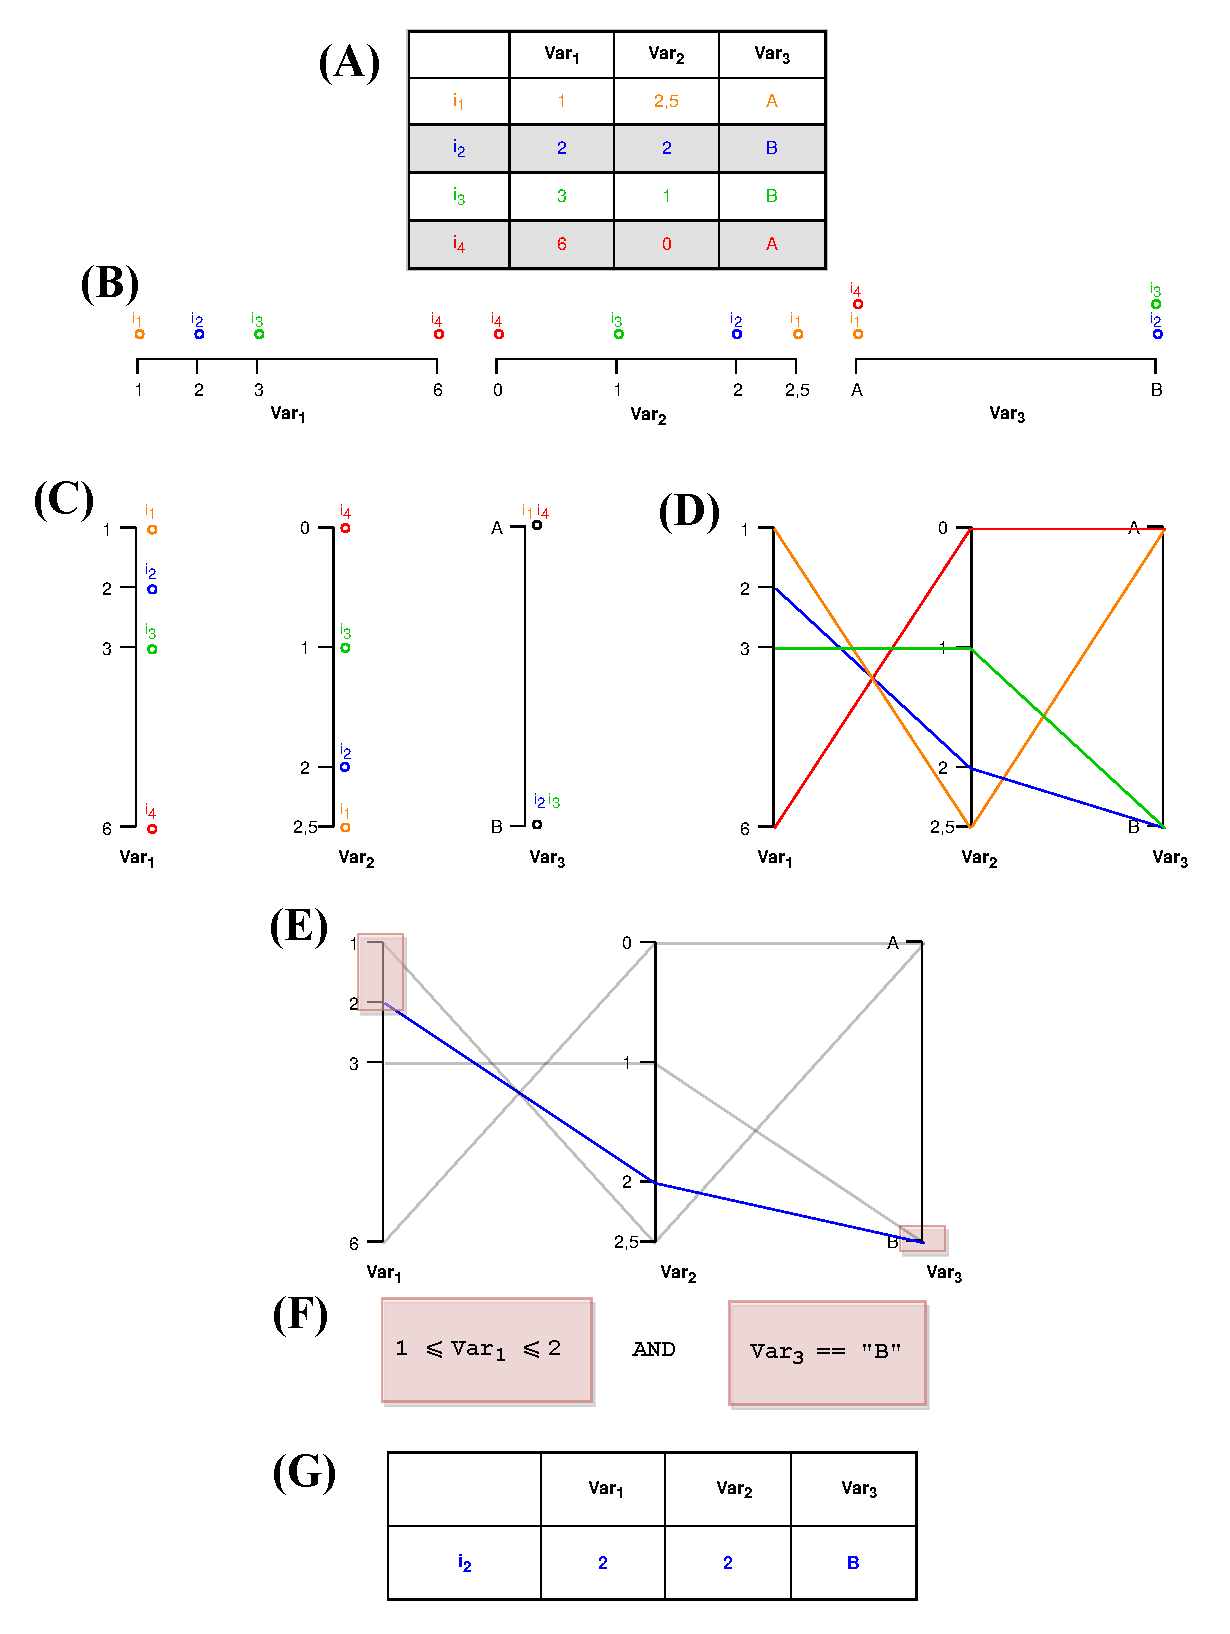
\includegraphics[width=.94\linewidth]{img/ParCoords_Brush.pdf}
	\caption{Construction d'un graphique en coordonnées parallèles et sélection interactive.\vspace{.1cm}}
	\label{fig:schema_parcoords}
	\end{figure}

	\end{encadre}


	Cette utilisation est aussi courante en géographie quantitative, et on la retrouve par exemple chez l'un des représentants de l'analyse spatiale des années 1990, Stewart Fotheringham.
	Cet auteur indique même l'usage du graphique en coordonnées parallèles en tant que filtre pour identifier des informations dans une autre dimension, spatiale ici : \og the data being displayed in parallel coordinates can be linked to a map and then brushed to highlight the locations of interesting lines displayed in \textit{m}-space on the parallel co-ordinates.\fg{} \autocite{fotheringham_trends_1999}.

	Appliqué aux données de SimFeodal, cette interface (\cref{fig:simvadb_dashboard}) se révèle particulièrement efficace pour sélectionner les configurations de paramètres à explorer.
	Ainsi, en \og brossant \fg{} quelques filtres manuellement (\cref{fig:simvadb_dashboard} - \textbf{A}), on arrive rapidement à isoler une expérience spécifique.

	\begin{figure}[H]
		\captionsetup{width=\linewidth}
		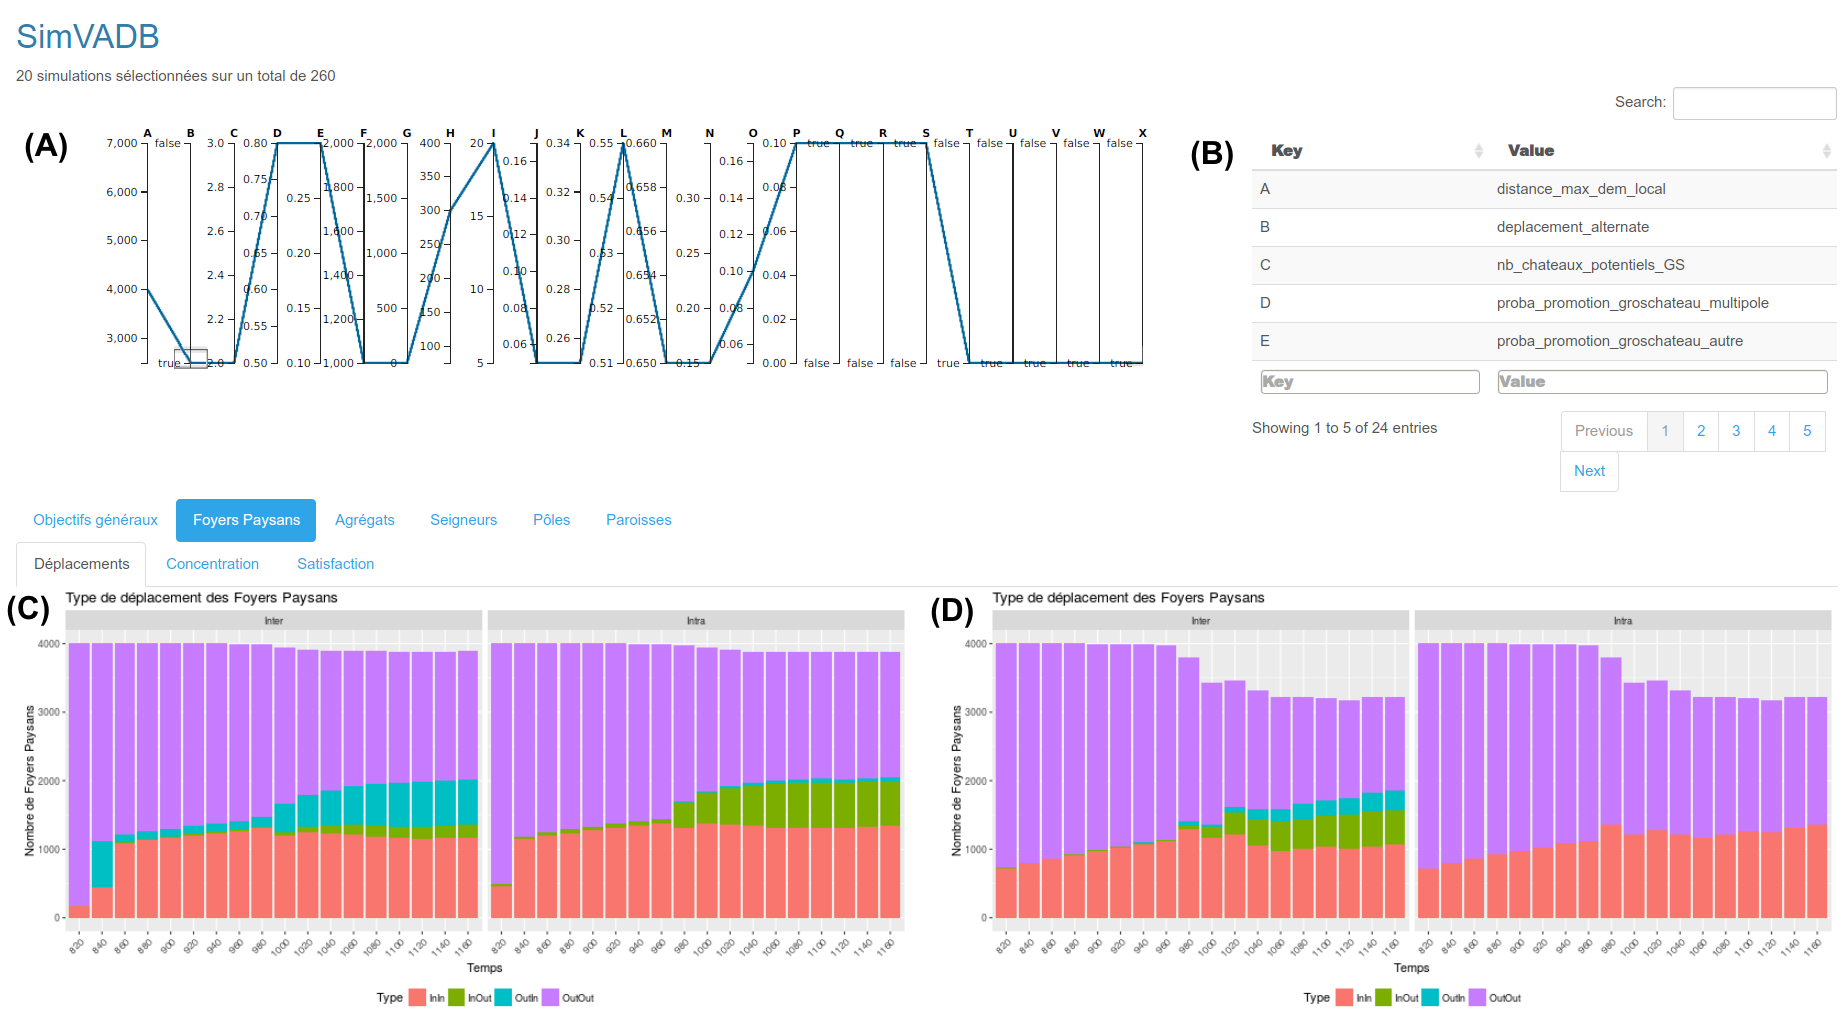
\includegraphics[width=\linewidth]{img/SimVADB_Dashboard2_annote_retouche.png}
		\caption{SimVADB (Simulation Visual Analysis DashBoard), un \textit{dashboard} d'exploration visuelle des indicateurs de sortie de simulation de SimFeodal.\\
		La sélection des simulations à explorer se fait dans le graphique en coordonnées parallèles (\textbf{A}), en \og brossant\fg{} des filtres graphiques sur les \og dimensions\fg{} du graphique, dimensions dont les intitulés sont explicités dans le tableau \textbf{B}.
		Les graphiques \textbf{C} et \textbf{D} indiquent l'évolution des types de déplacements des foyers paysans au cours des simulations.\\
		- Le graphique \textbf{C} représente, pour cet indicateur, une moyenne de l'ensemble des simulations intégrées dans la base de données (260 ici), recouvrant donc plusieurs valeurs de paramètres.\\
		- Le graphique \textbf{D} représente cet indicateur calculé depuis un sous-ensemble de 20 simulations (donc une expérience composée de 20 réplications), pour lesquelles le paramètre \og \textsf{B} \fg{} (\textsf{deplacement\_alternate}) vaut \textsf{true}.}
		\label{fig:simvadb_dashboard}
	\end{figure}

	Afin de permettre aux utilisateurs de remarquer les particularités des simulations explorées, nous avons choisi de mettre en emphase les différences entre la tendance générale des indicateurs, en calculant des moyennes de l'ensemble des simulations (\cref{fig:simvadb_dashboard} - \textbf{C}), et les valeurs spécifiques des indicateurs de l'expérience choisie (\cref{fig:simvadb_dashboard} - \textbf{D}).
	Cela permet, visuellement, d'être en mesure d'évaluer les sorties de simulation d'une expérience tout en ayant un référentiel visible.
	Les différentes expériences produisent des résultats sensiblement similaires\footnote{
		Si chaque expérience, et chaque réplication, produisent des résultats uniques, le choix d'une évaluation par des indicateurs visuels peut prêter à confusion si l'on n'a pas de repère précis.
		Les critères attendus, présentés dans \hl{le chapitre 3} sont ainsi assez précis pour départager une simulation très éloignée des attentes et une autre simulation plus conforme.
		Pour autant, par exemple quand les valeurs de paramètres varient faiblement, les résultats produits peuvent être assez similaires dans les grandes tendances qu'ils font ressortir.
	}, et on ne peut alors plus les comprendre sans les confronter à d'autres résultats similaires.
	Le choix d'une agrégation de l'ensemble des simulations effectuées est discutable, en ce qu'on aurait par exemple pu plutôt isoler des simulations \og de référence \fg{} afin de diminuer l'effet \og d'aplatissement \fg{} engendré par l'agrégation de résultats nombreux et hétérogènes.
	Toutefois, la variabilité des résultats étant encore assez restreinte, au moment de la création et de l'utilisation de SimVADB, ce référentiel agrégé permettait déjà une compréhension plus fine des sorties de simulations, en particulier dans l'analyse de l'impact de variations fines de valeurs de paramètres.

	\subsection{Explorer en comparant : SimEDB}\label{subsec:explorer-simedb}

	Après un travail de paramétrage grossier qui permet de stabiliser les mécanismes, il est souvent nécessaire de passer à une phase plus fine.
	On vise à ce moment à mieux calibrer un modèle à l'aide de variations de valeurs de paramètres de granularité inférieures.
	En vue d'évaluer les simulations, et donc de les différencier les unes des autres à l'aune des indicateurs générés, la comparaison d'une expérience spécifique avec un référentiel constitué de toutes les expériences précédentes ne permet plus de mener ce travail de comparaison fine.
	Les variations entre simulations sont trop fines pour être distinguables les unes des autres par le biais d'une comparaison avec un référentiel unique\footnote{
	On peut prendre l'exemple de SimFeodal.
	En faisant varier le nombre de foyers paysans de $4000$ à $4200$ ($5\%$ de variation), les résultats du modèle changent peu : de faibles variations de valeurs de paramètres entraînent le plus souvent de faibles variations dans les indicateurs de sorties observés.
	On peut de plus noter que les répercussions d'un changement de valeur de paramètre peuvent être très différentes de l'ordre de grandeur de ce changement de valeur.
	Cela s'explique par la non-linéarité de l'influence des paramètres.
	Dans l'exemple pris, pour ces $5\%$ de variation dans le nombre de foyers paysans, la majorité des indicateurs variera ainsi de moins de $1\%$.
	}.
	Cela s'entend quelque soit la manière dont ce référentiel est constitué, qu'il résulte d'une agrégation de simulations ou encore d'une version \og de base\fg{} du modèle (par exemple, dans le cas de SimFeodal, les versions principales identifiées dans le \hl{chapitre 4}).
	

	Pour pouvoir correctement évaluer les apports d'un nouveau jeu de valeurs de paramètres, et donc, dans une démarche itérative, pouvoir différencier deux expériences successives, il est nécessaire d'être en mesure de comparer directement les expériences les unes avec les autres, ou encore avec un référentiel facilement ajustable.
	On peut énumérer les quelques exemples de cas de figure suivants :
	\begin{itemize}
		\item Comparaison entre une expérience spécifique et une autre expérience spécifique de même \og importance\fg{}.
		Par exemple, comparer deux expériences qui font varier légèrement différement une valeur de paramètre.
		\item Comparaison entre une expérience spécifique et une autre expérience spécifique d'\og importance\fg{} différente.
		Cette différence de niveau peut être constituée par exemple par une version \og de base\fg{} que l'on comparerait à une variante de celle-ci.
		\item Comparaison entre deux expérimentations, par l'agrégation de leurs résultats.
		Si l'on a mené des expérimentations faisant varier de manière systématique deux paramètres différents, il peut être intéressant de les comparer en bloc, c'est-à-dire par exemple en prenant les moyennes de chacune des expériences composant ces expérimentations.
	\end{itemize}
	
	Ce faisant, on fait en fait varier la notion de \og simulation de référence\fg{}, qui peut alors revêtir plusieurs formes.
	Pour cela, il n'est plus possible de mener une comparaison visuelle entre un référentiel commun et une expérience spécifique, mais bien de baser l'évaluation sur la comparaison entre deux ensembles spécifiques qui doivent pouvoir être spécifiés.
	D'un point de vue méthodologique, cela requiert de pouvoir afficher conjointement les indicateurs de sorties de deux expériences (ou ensembles d'expériences).
	Cela implique aussi de laisser à l'utilisateur la responsabilité d'un choix supplémentaire puisqu'il faut désormais effectuer deux sélections : une pour chacun des points de comparaison.
	La sélection d'une expérience via l'usage de \textit{brushing} sur un graphique en coordonnées parallèles des valeurs de paramètres ayant montré son efficacité, il a été choisi d'étendre ce principe d'interactivité au choix du référentiel.
	
	Dans cette version remaniée de la plate-forme d'exploration (voir \cref{fig:simedb_villages}), renommée SimEDB\label{par:introduction-nom-simedb} (\textbf{Sim}Feodal \textbf{E}xploration \textbf{D}ash\textbf{B}oard)\footnote{
		\label{ftn:origine-simedb}
		La plate-forme d'exploration SimVADB (SimFeodal Visual Analysis Dashboard) a été renommée SimEDB ([...] Exploration Dashboard) par soucis de simplicité, le terme \og Exploration\fg{} nous semblant plus compréhensible et explicite que celui de Visual Analysis.
		Ce nom apporte de plus une cohérence sémantique entre plusieurs productions de l'auteur -- TimeLineEDB - \autocite{cura_timelineedb_2017}; RoadTrafficEDB et CitiBikeEDB - \autocite{cura_making_2017}.
		Cela inscrit cette plate-forme d'exploration de données issues de simulation dans une \og famille \fg{} d'outils d'exploration de données spatio-temporelles.
	}, l'accent est mis sur la comparaison de deux ensembles de résultats, chacun répondant à une sélection propre.
	L'utilisateur doit ainsi \og paramétrer\fg{} interactivement, via \textit{brushing}, les expériences à afficher pour le référentiel et pour les expériences à comparer.
	On dispose pour cela de deux outils de filtrage des simulations (partie de gauche dans la \cref{fig:simedb_villages}), qui peuvent être utilisés de concert, pour comparaison visuelle, ou par étapes successives\footnote{
		En menant par exemple une première comparaison entre une expérience \og A\fg{} en haut et \og B\fg{} en bas, puis en sélectionnant \og C\fg{} en haut, puis \og D\fg{} en bas etc.
		On compare ainsi A avec B, puis B avec C, et enfin C avec D.
	}.

	En superposant les graphiques et tableaux des indicateurs, la comparaison visuelle est facilitée.
	On peut alors comparer deux variations fines d'un mécanisme du modèle, en sélectionnant par exemple une unique différence dans les valeurs de paramètres du modèle (par exemple un paramètre relatif à la promotion des paroisses dans la \cref{fig:simedb_villages}).
	De manière générale, ce choix d'outil d'interrogation des données permet de répondre à l'ensemble des cas de figures identifiés dans les paragraphes précédents.
	
	\begin{figure}[H]
		\centering
		\includegraphics[width=\linewidth]{img/SimEDB_base_rotate.png}
		\caption{SimEDB }
		\label{fig:simedb_villages}
	\end{figure}

	\paragraph*{}
	Nous reviendrons plus précisément et longuement sur la description de SimEDB dans les parties suivantes (\cref{sec:SimEDB}, p. \pageref{sec:SimEDB}), mais après en avoir décrit les étapes de construction et les besoins auxquelles ces évolutions répondaient, il est maintenant nécessaire de revenir sur les données manipulées par cette plate-forme d'exploration.
	Le type, la structure et la masse de ces données (\cref{sec:sorties-simfeodal}) sont en effet indissociables des choix méthodologiques effectués pour SimEDB.
	Il est donc important de présenter les choix et contraintes de ces données avant d'entrer dans une description approfondie de la plate-forme.


\setcounter{section}{2}
\clearpage
\section{Organiser les données}\label{sec:organiser-donnees}

On a vu dans la première partie de ce chapitre (\cref{sec:sorties-simfeodal}) que les données produites par SimFeodal étaient nombreuses, diverses et massives.
La seconde partie (\cref{sec:explorer-sorties-simfeodal}) a montré les types de problèmes que de telles données, une fois exploitées pour en tirer les indicateurs de sortie, peuvent poser en matière d'exploration.

Nous souhaitons ici revenir sur une corollaire indispensable à l'utilisation efficace de ces données.
De la même manière que la multiplicité des indicateurs, des expériences et des expérimentations requiert des outils d'exploration adaptés, la multiplicité des données requiert des outils de stockage et d'interrogation eux aussi adaptés.
Là encore, on peut noter une succession de contraintes liées à ces données et à leur massification, contraintes qui limitent et guident les modes d'organisation de ces données.
Sans structuration adéquate, l'acquisition, l'archivage, l'interrogation ou encore la sauvegarde des données générées par le modèle ne peuvent être garantis, et encore moins de manière efficace.
Le choix d'une méthode d'organisation des données en sortie de simulations ne relève donc pas d'une quelconque coquetterie technique.
Au contraire, conditionne et contraint fortement aussi bien les modalités de création des indicateurs que les possibilités de la plate-forme d'exploration de les afficher de manière interactive.

%
%Contrairement à des modèles de simulations plus \og KISS \fg{}, par exemple les \og modèles-jouets\fg{} courants en Sciences Humaines et Sociales (\hl{ref Schelling/Sakoda, SugarScape, Prey-Predator, }), SimFeodal fait ainsi interagir de nombreux types d'agents, chacun doté de sorties spécifiques. Ces modèles sont le plus souvent évalués \og en direct\fg{}, les indicateurs présents dans l'interface des plate-forme de simulations suffisant à leur compréhension.
%La démarche suivie pour l'évaluation de SimFeodal repose sur des indicateurs visuels, qui doivent être examinés \textit{a posteriori} de leur production (\cref{subsec:observation-a-posteriori}), et l'évaluation du modèle ne peut être réalisée qu'en s'appuyant sur une part importante de ces sorties.
%
%Dans les modèles plus complexes utilisés en géographie (\hl{SimPop, MobiSim, SimPopLocal, MARIUS}), les données peuvent être plus massives (que ce soit intrinsèque au modèle (MobiSim) ou à sa méthode d'exploration (SimPopLocal)), mais leur structuration, souvent mono-agent, reste simple.
%Pour SimFeodal, où les indicateurs s'appuient parfois sur des requêtes croisant plusieurs types d'agents, la question de la structuration de ces données revêt une importance cruciale.




\subsection{Assurer la capacité d'interrogation des données}\label{subsec:capacite-interrogation}

Avant de se soucier du \og schéma\fg{} de la base de données\footnote{
	On utilise souvent le terme de \og schéma\fg{} pour désigner la version implémentée, dans un SGBD spécifique, du Modèle Conceptuel de Données (MCD).
	Contrairement au MCD, qui donne une version conceptuelle et générique d'une base de données, le schéma est donc tributaire du SGBD dans lequel il est intégré.
}, du choix du Système de Gestion de Base de Données (SGBD), ou encore des performances de ce dernier, il convient de se fixer sur la manière dont on souhaite entreposer les données.

De la myriade de fichiers issus de tableurs organisés dans une multitude de dossiers spécifiques à l'entrepôt de données décentralisé orienté documents, en passant par les traditionnelles bases de données relationnelles, les possibilités de stockage et d'organisation des données issues de simulations sont ainsi innombrables.
Plusieurs contraintes successives permettent de limiter le choix à un sous-ensemble de solution adaptées parmi lesquelles on peut alors mener une étude plus approfondie, passant notamment par des comparaisons entre ces candidats.

Une des premières contraintes est constituée par la nécessité d'interroger fréquemment et de manière répétée les données.
C'est l'une des contre-parties du passage d'un rapport automatique à un outil d'exploration interactif (\cref{subsec:dashboards}).
Ainsi, dans un rapport automatique, on interroge une fois les données pour en tirer les indicateurs de sortie, et ceux-ci ne sont plus amenés à changer, sauf re-calcul par exemple suite à des ajouts d'indicateurs.
Au contraire, dans un outil interactif, les indicateurs sont calculés depuis les données \og à la volée\fg{}, c'est-à-dire à chaque qu'un indicateur doit être affiché.
On peut mettre en place un système de cache, pour conserver les calculs déjà effectués, mais avec les dernières itérations de SimEDB où le nombre de possibilités de sélections est extrêmement important, ce n'est plus possible.
Il est nécessaire de procéder aux calculs à chaque affichage des graphiques et tableaux de résultats.
L'interrogation des données est donc extrêmement fréquente et répétitive.
Elle doit alors être aussi simple (en termes de mode d'interrogation) qu'efficace (en termes de rapidité d'interrogation).

Dans le cadre des données issues de SimFeodal, en vue de leur mobilisation dans SimEDB, nous avons ainsi eu à sélectionner quelques SGBD candidats parmi une foule de solution possibles.
Afin de guider ce choix, trois critères ont été définies, et forment, selon une hiérarchie propre à leur ordre, un ensemble de filtre ayant permis la réduction des SGBD possibles à un nombre appréhendable.
Ces critères, dont l'énonciation guidera cette partie, sont ainsi (1) l'universalité, ou \og agnosticité\fg{}, des SGBD aux outils de requête ; (2) la pérennité et stabilité des solutions disponibles et (3) les performances des SGBD considérés.

\subsubsection{Interroger de manière universelle et indépendante}

Lors de la conception d'un outil faisant appel à des données, qui plus est massives, il convient de se positionner tôt sur la manière d'interroger ces données.
Par interrogation, on entend ici, comme souvent dans le domaine des bases de données, la manière de faire appel, concrètement, aux données, pour en tirer les sous-ensembles, agrégations et autres résultats synthétiques résultant du traitement des données brutes.
Si l'on considère des données stockées dans un tableur, alors les \og formules \fg{}, les tableaux croisés dynamiques ou encore les graphiques issus du tableur sont des interrogations des données, qui s'expriment dans ce cas via un ensemble de langages, écrits -- les formules, qui font appel à des fonctions spécifiques des tableurs -- ou visuels -- les tableaux croisés dynamiques, construits en faisant glisser des intitulés de colonnes dans un tableau.

\paragraph*{Stockage distribué ou centralisé}\label{par:stockage-centralise}
Avant même de s'intéresser aux spécificités de ces langages, un premier choix réside dans le mode de stockage des données qui doivent être mis à disposition d'une plate-forme.
Doit-on laisser l'utilisateur intégrer lui-même les données, et ainsi, en faire un stockage \og distribué \fg{}, dans le sens où chaque utilisateur de l'application possèderait physiquement une copie locale des données ?
Ou, au contraire, les données doivent-elles être centralisées, c'est-à-dire enregistrées en une seule copie à laquelle les utilisateurs accèderaient à distance ?
Pour reprendre l'exemple des tableurs, doit-on privilégier une solution locale -- chacun ayant une copie du fichier tableur et menant ses propres modifications dessus -- ou une approche de type centralisée, par exemple en privilégiant des tableurs collaboratifs en ligne (\textit{Google Docs/Sheets} par exemple) ?

Habituellement, c'est-à-dire dans une grande majorité d'applications, les données sont stockées localement : cela permet, en particulier, de ne pas dépendre d'une connexion internet pour interroger des données qui seraient hébergées sur internet.
Dans le cas de SimFeodal, cette solution est rendue difficile, sinon impossible, par la masse de données en sortie de simulations.
Si chaque utilisateur de SimEDB devait posséder une copie des données, voir plusieurs en cas d'utilisations depuis différents ordinateurs, cela occuperait plusieurs gigaoctets de données à chaque fois.
De plus, en cas de mise à jour des données, c'est-à-dire d'insertions de nouvelles sorties de simulations, il faudrait distribuer à nouveau l'ensemble du jeu de données, à chaque fois.

Pour ces raisons, nous avons fait le choix d'un stockage centralisé, sous forme d'une architecture \og client-serveur\fg{}, hébergé sur un serveur internet dédié, ce qui permet à la plate-forme de travailler à chaque fois sur les données les plus à jour, réduit la taille du stockage physique associé, et dispense d'une configuration sur chaque poste utilisateur :
si le lien entre l'application et les données fonctionne correctement pour un utilisateur, il fonctionnera à l'identique pour tous les autres.
Ce choix présente un dernier avantage, non négligeable :
en stockant les données en un seul lieu, c'est-à-dire sur un serveur informatique, on peut faire en sorte de rendre ce serveur aussi performant que possible, et accélérer ainsi l'interrogation des données pour tous les utilisateurs.

\paragraph*{Interrogation spécifique ou générique}\label{par:interrogation-generique}

De nombreuses solutions intégrées de gestion de données proposent leurs propres modes d'interaction avec les données, c'est-à-dire un langage spécifique permettant d'interroger les données contenues dans le système\footnote{
	Souvent, cette interrogation se fait par appel à des \textit{API} (\textit{Application Programming Interface}, ou Interface de Programmation Applicative en français).
	Ces interfaces sont propres à chacune des plate-formes, et demandent donc un langage et un formalisme de requête spécifique.
}.
Au contraire, les SGBD les plus classiques s'appuient plutôt sur des langages de requêtes aussi standardisés que possibles, afin de faciliter l'adoption de leur propre solution à des utilisateurs d'autres plate-formes.
La spécificité présente l'avantage de langages plus adaptés aux données manipulées, et donc souvent plus intuitifs dans l'interrogation des spécificités des données.
De plus, la spécificité permet aussi une optimisation des requêtes, et est donc souvent plus performante que les solutions plus génériques.

De manière générale et dans le cas de SimFeodal, nous avons préféré privilégier une approche plus générique, faisant appel à des solutions de SGBD plus standardisées.
La raison tient principalement à une volonté de généricité du stockage des données : au cours des différentes étapes de construction de SimFeodal, les besoins en matières d'interrogation des données ont évolué.
Cette évolution était prévisible et prévue, et nous avons donc choisi dès le départ d'adopter uniquement des solutions modulaires, garantissant une évolutivité facilitée de la base de données, aussi bien regardant sa structure (enregistrement de nouvelles variables ou de nouveaux agents du modèle) que son contenu (massification des données en sortie au fur et à mesure de l'exploration du modèle).

De plus, dans la perspective de ce travail de thèse, où l'on cherche à rendre les productions aussi reproductibles et génériques que possible, il était indispensable de disposer d'un SGBD aussi standard que possible pour en faciliter l'adoption et l'adaptation à d'autres modèles de simulations par exemple.

\paragraph*{Bases de données relationnelles ou NoSQL}\label{par:sql-nosql}

Même une fois arrêté sur le choix de ne faire appel qu'à des outils standards pour stocker les données, le nombre de solutions disponibles demeure très important.
Afin de réduire ce nombre, on peut déjà choisir les grands types de SGBD auxquels faire appel.
Les SGBD sont ainsi souvent classés selon les grands traits de la méthode dont ils organisent les données.
Les deux grands types\footnote{
	Il en existe d'autres, comme les SGBD orientés objets (quasiment disparus aujourd'hui), orientés graphes (Neo4j\ldots), les SGBD pensés pour le stockage et l'interrogation d'ontologies (\textit{Triplestores RDF}, interrogeables en langage SPARQL) ou encore les nouveaux SGBD de type \og NewSQL \fg{} (Apache Ignite, CockRoachDB\ldots) pensés pour une parallélisation massive des données. Ces types de SGBD ne correspondent toutefois pas du tout aux besoins identifiés pour SimEDB/SimFeodal, et sont en général dédiés à des problèmes et marchés de niches. Nous ne les décrirons donc pas plus en détail ici.
} sont les SGBD \og relationnels\fg{} et les SGBD \og NoSQL\fg{}.
Si la distinction est sujette à de très nombreux débats, souvent virulents
\footnote{
	À l'instar des violentes querelles qui agitent régulièrement les informaticiens : Vim vs Emacs, Programmation Orientée-Objet vs Programmation Fonctionnelle, R vs Python\ldots
}
, on se contentera ici de définir les SGBD relationnels comme les SGBD, les plus fréquemment utilisés, où l'information est stockée dans des tables composées de champs -- les colonnes, correspondant aux variables -- et de lignes -- les entités décrites par les variables.
Le format des données est donc rectangulaire et n'accepte pas, comme dans un tableau statistique, que les entités possèdent un nombre de variables différent, ou encore des types de valeurs différents de celles des autres entités (une même colonne ne peut donc contenir conjointement un nombre et un texte dans des lignes différentes).
On nomme ces bases de données relationnelles via la manière qu'elles ont de faire communiquer des éléments hétérogènes, et donc contenus dans des tables différentes : si les tables ont une colonne en commun, on pourra alors effectuer une opération de jointure permettant de mettre en commun les informations de ces tables dans une unique table résultante.

A l'inverse, les SGBD NoSQL se définissent de manière opposée à ce mode de stockage\footnote{
	À l'origine, c'était le sens fort du nom \og NoSQL \fg{} : Non SQL, le SQL faisant ici références aux SGBD pré-existants, majoritairement relationnels, dont la mouvance NoSQL, portée par l'apparition des \og \textit{big data} \fg{} a voulu se distinguer.
	Sans entrer dans le détail, notons tout de mêmes que de nombreux SGBD NoSQL, qui traduisent désormais cet acronyme par \og Not only SQL\fg{}, sont maintenant relationnels, mais mettent en avant d'autres types d'approches.
}, rompant par exemple la contrainte d'unicité de type des colonnes, ou de nombre identique de colonnes renseignées pour chaque entité. Pour simplifier le discours, on se contentera de caractériser les SGBD NoSQL comme des SGBD non relationnels.
Les SGBD NoSQL ont, en général, de bien meilleures performances et une plus grande flexibilité que les SGBD relationnels.
Dans le cas de SimEDB/SimFeodal, où l'on est confronté à des données massives, cela présente un avantage non négligeable.

Toutefois, leur flexibilité est associée à une contrainte majeure en termes de généricité : alors que les SGBD relationnels partagent un langage d'interrogation commun, le SQL (\textit{Structured Query Language})\footnote{
	Ce langage d'interrogation est omniprésent dans l'interaction avec les SGBD, mais aussi, avec de légères variantes, au sein de nombreux logiciels reposant des sélections de données, par exemple les logiciels SIG qui se basent sur la syntaxe du SQL (le fameux triptyque \texttt{\textbf{SELECT} \ldots~\textbf{FROM} \ldots{} \textbf{WHERE} \ldots})
}, les SGBD NoSQL font plus souvent appels à des langages spécifiques à chaque SGBD.
Pour SimEDB, cela impliquerait une fort dépendance au SGBD choisi : en cas de changement de SGBD, toutes les requêtes seraient à reformuler dans le nouveau langage, parfois même selon des logiques extrêmement différentes les unes des autres (dérivés du SQL, interrogations via des objets JSON, via des langages de parcours de graphes\ldots{}) etc.
Au contraire, avec les SGBD relationnels, le langage de requête étant commun, une fois le code d'interrogation généré, il est très aisé de changer de SGBD cible.
Cela garantie une forte capacité d'évolutivité aux outils d'interrogation de données tels que SimEDB.
Puisque les fournisseurs de données sont interchangeables, on peut en changer au fur et à mesure de l'apparition de nouveaux besoins.

En raison de la généricité de ces solutions relationnelles, qui vient s'ancrer dans la recherche de reproductibilité et de généricité de notre démarche d'ensemble, nous avons donc choisi de faire reposer le stockage et l'interrogation des données sur des SGBD relationnels.
Cette décision s'est montrée d'autant plus heureuse que, au cours de la construction et de l'évolution de SimEDB, le SGBD choisi pour héberger les données a changé plusieurs fois.
La généricité des outils choisis a permis de minimiser, voire quasiment d'éviter, les changements à apporter au code-source de SimEDB relatif à l'interrogation de données en vue de produire les indicateurs de sortie depuis les données brutes en sortie de SimFeodal.


\paragraph*{Entrepôts de données et interrogation directe}\label{par:interrogation-directe}

En parallèle des SGBD, des solutions \og intermédiaires\fg{} permettent de s'abstraire des SGBD en eux-mêmes pour mener les requêtes.
Ces solutions, que l'on nomme \og Entrepôts de Données\fg{} (\textit{Data Warehouses}), se comportent comme une surcouche faisant l'interface entre un ou plusieurs SGBD et la requête émise par le client final.
Elles se placent donc comme intermédiaire entre les SGBD mobilisés et les applications qui les interrogent.
Les entrepôts de données jouent aussi bien le rôle d'agrégateurs de données\footnote{
	C'est-à-dire qu'ils permettent d'agréger des sources de données composites, provenant potentiellement de différentes sources (plusieurs bases de données relationnelles) et de différents types de sources (différents SGBD, relationnels ou non par exemple).
} que d'environnements de manipulation et de restructuration de données (on les nomme alors \og ETL\fg{} -- \textit{Extract-Transform-Load}).

Le grand intérêt de ces outils d'interface est d'abstraire la complexité de chacune des bases de données manipulées en générant une interface d'interrogation unique et générique, souvent performante grâce à des optimisations spécifiques (pré-calcul des requêtes possibles par exemple).

\hl{Dans les paragraphes suivants, Lena note qu'elle a perdu le fil mais que c'est bien écrit.}

Dans le domaine de la visualisation interactive de données, ces outils sont beaucoup utilisés, en particulier dans le monde de l'informatique décisionnelle.
Ils se révèlent en effet extrêmement utiles quand les données sources ne peuvent être modifiées (par exemple quand elles sont issues de chaînes de collecte complexes, ou encore quand leur volumétrie et leur débit est important), puisqu'ils permettent de constituer une surcouche rendant l'interrogation et la visualisation de ces données accessibles à des analystes non spécialistes de la manipulation de données.
Toujours en informatique décisionnelle, il est courant de faire appel à des entrepôts de données d'un type spécifique, les \og traitements analytiques en lignes\fg{}, ou environnements OLAP (\textit{\textbf{O}n\textbf{L}ine \textbf{A}nalytical \textbf{P}rocessing}), qui permettent de structurer, par exemple sous formes de cubes de données, des sources de données hétérogènes présentant de nombreuses dimensions.

Les environnements OLAP ont été utilisés, promus et adoptés dans le champs scientifique de la géomatique, en ce qu'ils permettent de mettre en place rapidement des environnements d'analyse visuelle de données multi-dimensionnelles spatiales et temporelles.
Dans ce cadre, où ces outils sont appelés \og SOLAP\fg{} (\textit{Spatial OLAP}), les données spatiales s'intègrent extrêmement bien en raison de leur capacité à s'emboîter selon les échelles, ouvrant dès lors la voie à des analyses multi-échelles et multi-dimensionnelles complexes.

Dans la communauté géomatique francophone, les solutions SOLAP sont bien représentées (par exemple autour de Sandro Bimonte et de son travail de visualisation de données spatiales environnementales,  \autocite{bimonte_integration_2007, bimonte_towards_2005, zaamoune_new_2013}, et sont couramment employées pour répondre à des questionnements méthodologiques proches de ceux développés dans cet ouvrage.
En lien avec les besoins de performances identifiés plus haut, on notera que certaines solutions OLAP permettent aussi d'optimiser la vitesse d'interrogation de bases de données, et visent ainsi à garantir une réponse rapide pour des outils d'interrogation de données interactifs \autocite{zeng_iolap_2016}.

Nous avons cependant choisi de ne pas faire usage de ces outils pour les mêmes raisons que pour les SGBD NoSQL : les avantages qu'ils présentent ne suffisent pas à contre-balancer les défauts en termes de généricité qu'ils introduisent. Pour profiter au mieux de ces environnements, il est en effet nécessaire de faire appel à un nouveau langage d'interrogation des données (le \og MDX\fg{}, de \og \textit{Multidimensional Expressions}\fg{}).
Les différentes solutions OLAP/SOLAP, de plus, présentent les mêmes inconvénients que les SGBD NoSQL : chacune interagit de manière propre aux différents SGBD, et ces outils sont donc difficilement interchangeables.

De la même manière, on se restreindra, parmi les SGBD relationnels interrogeables en SQL, à ceux qui disposent d'une méthode d'interrogation standard : si tous ces SGBD acceptent le SQL, certains demandent par exemple des protocoles spécifiques pour recevoir établir la connexion au SGBD, recevoir la requête et renvoyer les données correspondantes.
Pour ce même choix \og d'agnosticité \fg{} de la plate-forme d'interrogation face à la solution de stockage choisie, on ne conservera que les SGBD acceptant les connexion standardisées (ODBC et JDBC).

\paragraph*{SGBD et données spatiales}\label{par:sgbd-spatial}

On a mentionné le fait que les entrepôts de données étaient fortement utilisés, en particulier dans la communauté géomatique, car très appropriés aux données spatiales.
De prime abord, ce point peut paraître critique : jusque là, on s'est contenté de mentionner les capacités organisationnelles de SGBD, et non leur aptitude à manipuler des données spatiales.
Ce point, dans les SGBD relationnels, constitue un filtre important : sur la centaine de solutions disponibles, seule une poignée est en mesure de stocker efficacement et d'interroger de l'information spatiale \footnote{
	Les données spatiales peuvent être stockées dans tous les SGBD si l'on attribue une représentation textuelle, en chaînes de caractères, par exemple en utilisant le format \textit{Well-Known Text} (WKT).
	Pour autant, ce format est lourd, inadapté à une indexation, et ne peut permettre à un SGBD de mener des requêtes spatiales directement depuis ces entités.
	Il est ainsi, par exemple, impossible de calculer le centroïde d'un polygone directement depuis une représentation WKT, alors que c'est aisé avec un stockage géométrique.
}.

Pourtant, au regard des indicateurs de sortie de simulation sur lesquels on s'appuie pour évaluer le comportement de SimFeodal, une grande majorité est non spatiale, en raison de la difficulté à agréger des données spatiales théoriques.
Dans SimFeodal, la plupart des indicateurs de sortie sont non spatiaux, c'est-à-dire qu'ils mobilisent plus la dimension attributaire des données que leur dimension géographique\footnote{
	Les raisons en sont multiples et on y reviendra largement dans le \hl{chapitre 7}.
	Notons tout de même que les indicateurs résultent de l'agrégation des réplications, et que cette agrégation est extrêmement complexe sinon impossible sur des données spatiales majoritairement aléatoires (voir \hl{chapitre 2, section 2.2.2.1}).
}.

La gestion de données spatiales ne constitue donc pas une absolue nécessité, contrairement aux points évoqués auparavant.
Elle peut toutefois se révéler avantageuse, ne serait-ce que pour permettre l'observation des configurations spatiales simulées.
Cela constitue une approche idiographique, visant à exemplifier plus qu'à synthétiser, mais permet tout de même une compréhension rapide des changements de structures spatiales.
Toutes choses égales par ailleurs, on privilégiera donc des solutions de stockage ayant une capacité à gérer les données spatiales.

\paragraph*{}
Pour héberger et organiser les données produites par SimFeodal, en vue de leur interrogation dans SimEDB, nous avons choisi de restreindre la myriade de solutions disponibles grâce à plusieurs filtres successifs.
En premier lieu, on a choisit de faire appel à des solutions centralisées (\nameref{par:stockage-centralise}), au sein de Systèmes de Gestion de Base de Données (SGBD).
Ces SGBD permettent une interrogation standardisée (\nameref{par:interrogation-generique}) via un langage de requête universel, le SQL (\nameref{par:sql-nosql}).
On a ensuite décidé d'interroger ces SGBD sans passer par l'intermédiaire d'entrepôts de données, et au travers de connexion aussi standardisées que possible (\nameref{par:interrogation-directe}).
Les SGBD répondant à ces critères sont les SGBD \og relationnels \fg{}, dont certains possèdent qui plus est une capacité intéressante à stocker et interroger des données spatiales (\nameref{par:sgbd-spatial}), ce qui constitue notre dernier filtre.

\subsubsection{Interroger de manière robuste et efficace}\label{subsubsec:interroger-robuste-efficace}

En dépit de l'accumulation de critères exposée précédemment, une quantité importante de SGBD demeurent en lice.
Afin de les différencier, nous avons choisi d'ajouter des critères qui ne portent plus sur les grands types de SGBD, mais plutôt sur une différenciation des SGBD relationnels existants.
Ces deux critères, précisés par la suite, sont d'une part la robustesse des SGBD, et d'autre part leurs performances.
Ces critères sont pas des \og prétextes \fg{} à une hiérarchisation quantifiée des SGBD, mais ont une importance prépondérante dans notre cas d'utilisation.

\paragraph*{Robustesse des SGBD}
Le premier critère ajouté est celui de la robustesse, c'est-à-dire, ici, de la capacité du SGBD à être interrogé de manière (1) stable et  (2) pérenne dans le temps.
Une même requête sur les mêmes données doit systématiquement renvoyer le même résultat (stabilité), quelle que soit la durée séparant ces requêtes (pérennité).
Si la base de données n'est plus interrogeable quelques mois après sa configuration, ou qu'elle renvoie des résultats différents, alors elle ne peut constituer une solution crédible à l'exploration d'un modèle sur une période longue.

La \textbf{stabilité} des bases de données est principalement due à la manière de stocker l'information d'un point de vue informatique.\\
En premier lieu, l'information peut être contenue \og en clair\fg{} ou alors de manière archivée.
Un stockage \og en clair\fg{} est plus facilement accessible, puisqu'on peut le consulter avec n'importe quel éditeur de texte.
Un stockage archivé est moins universel, mais occupe généralement un espace disque inférieur et comporte des mécanismes de vérification de la cohérence des données.
Il est donc plus stable.\\
Une second différenciation tient à l'emplacement lieu du stockage.
Celui-ci peut être effectué dans un unique fichier, ce qui a l'immense avantage de la portabilité des données : pour faire migrer ou sauvegarder la base de données, il suffit de copier le fichier.
La plupart des SGBD adoptent toutefois un mode d'organisation en plusieurs fichiers, notamment pour des questions de redondance et de vérification de l'intégrité des données : en multipliant les fichiers, on minimise le risque d'erreur critique sur l'ensemble des fichiers à la fois.
On notera enfin un dernier type de SGBD, où l'information n'est pas stockée sur un disque dur, mais est entièrement contenue dans la mémoire vive de l'ordinateur : les SGBD \og \textit{in-memory}\fg{}.
Ces SGBD sont les plus rapides et stables, mais il faut les re-constituer à chaque redémarrage du serveur qui les héberge, ce qui peut prendre un temps important.

L'enjeu du choix est de se prémunir de \og corruptions\fg{} de la base de données : quand le SGBD ne comporte que pas ou peu de mécanismes de vérification de l'intégrité ou de la cohérence des données, il peut arriver qu'une base de données se corrompe.
On peut prendre l'exemple de l'exécution d'une requête demandant un calcul complexe et long.
Cette requête pourrait être interrompue en cours d'exécution par faute d'un \textit{bug} ou d'une expiration de sessions (\textit{timeout}). Dans ce cas, il se peut que la base de données s'arrête dans un état muté -- avec une nouvelle table ajoutée pour moitié par exemple -- et ne soit donc plus intègre.
C'est très fréquent pour les SGBD basés sur un unique fichier, ou encore stockés en clair, puisque les nouvelles informations de la base de données y sont ajoutées au fur et à mesure, plutôt que d'être intégrées dans un fichier annexe que l'on pourrait réinitialiser en cas d'erreur.\\
Avec la volumétrie des données produites par SimFeodal, les requêtes peuvent s'avérer très longues, et une erreur dans une requête peut fréquemment corrompre la base de données.
En termes de stabilité, on se tournera donc plutôt vers des SGBD relationnels stables, basés sur une redondance des données et donc sur des architectures archivées et multi-fichiers.


La \textbf{pérennité} des SGBD est un sujet proche, tenant aussi à la capacité à interroger les données contenues dans une base de données, mais cette fois-ci du point de vue de l'interrogation en elle-même plutôt de des données sur lesquelles elle s'applique :
si le SQL est un langage standard\footnote{
	Dans les faits, on notera tout de même qu'il existe plusieurs normes successives, des \og révisions\fg{} du SQL, qui apportent chacune leur lot de subtilités dans l'usage du langage.
	Les SGBD interrogeables en SQL ne disposent donc pas toutes des mêmes fonctionnalités, selon la révision du SQL qu'elles respectent.
}, les types de données intégrées varient cependant d'un SGBD à un autre (champs textuels ou d'entiers \og courts\fg{} par exemple).
SQL étant un langage typé, selon la manière (bas niveau) dont sont intégrées les données, certaines requêtes identiques peuvent renvoyer des résultats différents selon les SGBD.
Plus gênant, les normes implémentées peuvent varier d'une version à l'autre d'un SGBD.
Un SGBD relationnel respectant strictement la norme SQL pourrait ainsi évoluer pour supporter plus de fonctionnalités, par exemple en ajoutant des fonctions plus récentes (fenêtres glissantes, ajouts en masse etc.), et renverrait dès lors des résultats différents selon les versions.
Pour les SGBD les plus employés, le nombre d'utilisateurs garantit une rétro-compatibilité des requêtes.
Pour les SGBD de moindre envergure cependant, par exemple les plus performants et récents issus de la recherche en informatique, cette rétro-compatibilité n'est pas du tout garantie.

Comme souvent en matière d'infrastructure informatique, il est donc nécessaire de tenir compte d'un compromis entre l'ancienneté et la forte adoption de certains SGBD d'une part, et les facilités et gains de performances amenées par les plus récents d'autre part.
Dans le cas des données de SimFeodal, en tenant compte de cet inévitable compromis, nous avons choisi de privilégier des SGBD reconnus, soient-ils anciens et fortement adoptés ou plus récents mais utilisés par des acteurs d'envergure\footnote{
	La liste des solutions envisagées, ensuite comparées à l'aube de leurs performances, est visible dans l'axe des ordonnées de la \cref{fig:db-benchmarks}.
}.
Ce faisant, on se coupe immanquablement de solutions extrêmement intéressantes et performantes\footnote{
	Par exemple BlinkDB \autocite{agarwal_blinkdb_2013}, qui permet de limiter une requête à un temps maximal d'exécution donné : quand la requête n'est pas complète, le SGBD renvoi une estimation du résultat, estimation qui gagne en précision quand on augmente la limite temporelle.
	Un SGBD de ce type serait extrêmement précieux en \textit{visual analytics}, mais la jeunesse de cet outil ainsi que sa nature de projet de recherche rendent incertain la continuité de son développement dans le temps.
	En 2018, le projet semble d'ailleurs avoir été abandonné\ldots
}.
Ce choix est toutefois en la large faveurd'une meilleure garantie de pérennité, et de robustesse en générale, des données de SimFeodal.

\paragraph*{Performance des SGBD}

Une fois que les solutions disponibles ont été discriminées par leur type, par leur interface avec les requêtes et par leur robustesse, la quantité de SGBD restant demeure de l'ordre de la dizaine.
Pour choisir, parmi ceux-là, le SGBD qui sera le plus adapté aux besoins identifiés, il est donc nécessaire d'établir des critères plus précis et quantifiables.
Dans le cas d'une application interactive, c'est-à-dire où le nombre de requêtes émises au cours d'une session d'utilisation peut être importante, les performances des SGBD constituent un critère majeur pour départager l'ensemble des SGBD considérés.

Il est difficile de qualifier les \og performances\fg{} d'un SGBD : on entend en fait par ce terme un vaste ensemble hétérogènes de propriétés.
On peut par exemple juger les performances par le filtre de la mémoire occupée par le stockage d'une base de données, ou encore par le nombre de requêtes concurrentes que peut gérer un SGBD, ou encore par la capacité à paralléliser le stockage sur plusieurs serveurs.
Dans notre cas, ces points sont assez peu significatifs : en dépit de la quantité de sorties, l'ordre de grandeur -- quelques gigaoctets de données -- reste largement entreposable sur un environnement classique, sans besoin de parallélisation.
De la même manière, SimEDB est un environnement dédié à des utilisateurs experts, en petit nombre : les chercheurs travaillant autour de SimFeodal.
La quantité de requêtes simultanées ne peut donc pas dépasser la dizaine, ce qui constitue une trivialité pour l'ensemble des SGBD relationnels classiques.
On s'attachera donc à juger les performances en matière de rapidité d'exécution des requêtes.
Il ne s'agit pas ici de choisir un SGBD qui ferait gagner quelques millisecondes par rapport à un autre, mais plutôt de discriminer les SGBD présentant une durée de réponse trop importante pour notre usage.

En effet, plus les données sont massives, plus le temps d'exécution d'une requête augmente, souvent sous la forme d'une fonction puissance.
Si tous les SGBD présentent des vitesses acceptables et proches sur des bases de données de faible volume, l'écart s'accroît considérablement à mesure que les données s'accumulent.
La \cref{fig:db-benchmarks}\footnote{\label{ftn:dataset-exemple}
	Dans cette figure, on compare la rapidité de différentes requêtes sur un jeu de données identique selon les SGBD.
	Ce type de test de performance permettant la comparaison de solutions techniques diverses est appelé \textit{benchmark}.
	Ce jeu de données, composé de 100 Millions de lignes et de deux colonnes numériques, présente une volumétrie comparable (franchement inférieure en nombre de colonnes toutefois) à celle des données issues de SimFeodal qui sont interrogées dans SimEDB.
} montre les différences incontestables qui existent entre les SGBD étudiés. On peut y constater que l'écart est gigantesque, par exemple vis-à-vis du temps nécessaire à une jointure, entre les 4 secondes de MonetDB et les 300 secondes (5 minutes\ldots) de SQLite.
Le choix d'un SGBD selon ses performances a donc un impact majeur sur la fluidité d'une application d'exploration de données massives.
Pour départager les SGBD, on comparera leurs performances selon les différents types d'opérations demandées, qu'elles concernent l'écriture dans la base (insertion) ou des types de lecture (agrégation et jointure).

\clearpage
\subparagraph{Performances en écriture et en lecture}

La \cref{fig:db-benchmarks} affiche des résultats qui semblent globalement ordonnés (les quatre premiers SGBD sont par exemple quasiment toujours plus lents que les 2 derniers), mais fluctuent cependant à la marge selon les opérations demandées.
La première colonne du graphique montre ainsi le temps nécessaire à l'insertion du jeu de données exemple (voir la note de bas de page \ref{ftn:dataset-exemple}) dans le SGBD depuis un fichier CSV.
Les deux colonnes suivantes exposent le temps nécessaire au traitement d'une requête, donc à une interrogation des données une fois archivées dans les bases de données.
On peut constater que le classement des SGBD varie faiblement en lecture, et de manière assez faible en insertion : les deuxièmes et troisièmes colonnes respectent un ordre globalement similaire, assez différent de celui de la première colonne.
Dans un environnement classique, la performance d'insertion de données est un facteur prépondérant : quand de nouvelles données sont ajoutées constamment, par exemple pour stocker des données issues de capteurs automatiques, l'insertion peut vite constituer le goulot d'étranglement de la solution.

Pour SimFeodal, l'insertion n'est pas véritablement un enjeu : les données sont ajoutées par bloc, manuellement, une fois que des nouvelles simulations ont été exécutées.
C'est donc au pire un acte quotidien, mais dans ce cas, que la requête demande 10 secondes (MapD) ou 10 minutes (MySQL InnoDB), cela n'a que peu d'impact.
La première colonne est donc un indicateur de performance peu adapté dans notre cas.

Les deux colonnes suivantes, relatives à l'interrogation de données, se révèlent au contraire extrêmement importantes : à chaque action de l'utilisateur de SimEDB, une nouvelle requête est envoyée pour calculer un nouvel indicateur correspondant au jeu de données filtré manuellement (cf. \cref{subsec:explo-interactive}).
À chaque affichage d'onglet, une nouvelle requête est donc émise et traitée. Même si tous les indicateurs ne sont pas systématiquement mobilisés -- et donc calculés -- (cf. \hl{chap 3}), cela signifie tout de même que pour chaque sélection, une bonne dizaine d'indicateurs seront observés, et donc, autant de requêtes.
Quand une requête demande 60 secondes (par exemple PostgreSQL en \og jointure\fg{}), cela implique que chaque indicateur requiert au moins une minute avant de s'afficher.
Pour observer une dizaine indicateurs, l'utilisateur devra donc attendre patiemment une dizaine de minutes, sans même tenir compte du temps qu'il passera à les analyser visuellement.

Pour noircir le trait, notons de plus que les résultats communiqués dans la \cref{fig:db-benchmarks} correspondent à des requêtes simples qui ont valeur d'exemples de base.
Dans le cas de SimEDB, le calcul des indicateurs requiert des requêtes plus complexes, faisant appel à des agrégations et à des jointures en même temps, et les délais affichés dans ce \textit{benchmark} sont donc bien inférieures aux durées éprouvées en conditions réelles au sein de SimEDB.


\begin{figure}[H]
	\centering
	\includegraphics[width=\linewidth]{img/benchmark_results.pdf}
	\captionsetup{width=.95\linewidth}
	\caption[Comparaison de la performance de différents SGBD sur un jeu de données test de 100 millions de lignes.]{Comparaison de la performance de différents SGBD sur un jeu de données test de 100 millions de lignes. 
		Résultats tirés de \textcite{pafka_benchm-databases_2017} et complétés par l'auteur.\\
		Les \og types de Bases de Données\fg{} correspondent aux usages les plus fréquents des SGBD comparés :\\
		- Analytiques : SGBD optimisés pour les traitements de type agrégation, via une architecture orientée colonne plutôt qu'orientée ligne comme dans les SBGD Relationnels. Ils sont optimisés pour la rapidité d'exécution.\\
		- Massives : SGBD pensés pour la gestion et l'interrogation de données massives (big data), permettant notamment une parallélisation des requêtes. Ils sont optimisés pour la capacité à gérer des volumes gigantesques de données.\\
		- Statistiques : SGBD internes aux environnements de traitement de données statistiques, reposant sur une gestion en mémoire vive.
		Souvent intégrés d'office dans les environnements décrits (R, Python), ce sont les SGBD les plus simples à mettre en place et à manipuler.
	}
	\label{fig:db-benchmarks}
\end{figure}

\subparagraph{De l'intérêt de gagner quelques secondes}

La \cref{fig:db-benchmarks} permet d'isoler un sous-ensemble de quatre SGBD ayant, avec le jeu de données testé, des réponses inférieures à une dizaine de secondes : Spark avec cache, MonetDB et MapD sur CPU ou GPU.
On pourrait se contenter de choisir le SGBD le plus complet parmi ces quatre solutions.

Pourtant, un autre domaine d'étude appuie l'importance relative des écarts, mêmes faibles, dans les durées de requête.
Ce domaine est celui des sites internet, où les requêtes servent à générer le contenu de différentes pages en interrogeant des base de données de contenu.
La consultation d'un site internet consiste à charger plusieurs pages, pour l'utilisateur.
Du point de vue du serveur, chacune des pages demandées par l'utilisateur requiert différentes requêtes à des bases de données.
La navigation dans un site est donc assez comparable à l'utilisation d'une application d'exploration de données : des requêtes hétérogènes, plus ou moins lourdes, s'y succèdent et visent à filtrer et mettre en forme, de manière explicite, des extraits d'informations stockées dans des bases de données.
Plusieurs études ont montré que la durée d'affichage d'une page web jouait de manière considérable sur l'usage d'un site, composé de plusieurs de ces pages.
L'étude la plus parlante est décrite par \citeauteur{patel_speed_2011} qui relate une expérience vécue au sein du moteur de recherche Google  :\vspace{-0.5cm}

\begin{quotation}
	\og
Google did an interesting experiment with regard to load times. Google Vice President Marissa Mayer asked web surfers – would you rather see 10 or 30 results for your Google search? The users agreed that 30 results per page sounded like a good idea. So Google implemented it on some results pages.
Then the shock came.\\
Pages that displayed 30 results each had traffic to them drop an astounding 20\%. Google tested the loading difference between the 10 and 30 results pages and found that it was just \textbf{half of a second}. If half of a second made that much of a difference in how long users were willing to wait, how much of a difference could it make to your site if you carved a second or two off of load time?
	\fg{}\\
	\mbox{}~ \hfill  \autocite{patel_speed_2011}
\end{quotation}\vspace{-0.5cm}

Si l'environnement et les conditions décrites ne sont pas directement comparables avec celles de SimEDB, il demeure qu'une différence même faible dans un temps de chargement, ou, pour SimEDB, dans un temps d'affichage d'un indicateur de sortie, pourrait avoir des conséquences négatives pour l'utilisation de la plate-forme.

Un autre exemple appuie ce raisonnement et répond à la dernière interrogation de \citeauthor{patel_speed_2011}, dans un cadre un peu plus proche de SimEDB.
\citeauteur{elliott_how_2017}, employée d'une société qui propose des solutions d'accélération de sites web, a réalisé un rapport sur les perte d'audience des sites webs en fonction du temps de chargement des pages \autocite{elliott_how_2017}.
Les résultats de son étude sont présentés dans la \cref{fig:page-abandon}, et permettent de quantifier un effet bien connu, qui veut que l'utilisateur quitte plus rapidement un site (et en visite donc moins de pages) quand les pages sont plus longues à charger.

\begin{figure}[H]
	\centering
	\includegraphics[width=.9\linewidth]{img/abandon_pages.pdf}
	\caption{Impact du temps de chargement d'un site web sur sa consultation. D'après \textcite{elliott_how_2017}.}
	\label{fig:page-abandon}
\end{figure}

Cet exemple est plus directement comparables aux contraintes de SimEDB.
Chaque consultation d'un indicateur de sortie correspond ainsi à la vue d'une page dans cet exemple.
Ces chiffres renforcent l'importance à accorder au temps de chargement des indicateurs, et donc à la durée de l'exécution des requêtes qui les génèrent.
Quelques secondes de différence dans le chargement suffisent ainsi à réduire drastiquement le nombre d'indicateurs que l'utilisateur acceptera d'analyser.

On peut toutefois pondérer ces comparaisons et minimiser l'importance d'écarts de l'ordre de grandeur de la seconde.
Dans le cas de SimEDB, contrairement à celui d'un site web ou d'un moteur de recherche, l'utilisateur est \og captif\fg{}.
Cela signifie qu'un thématicien souhaitant explorer les résultats produits par SimFeodal n'aura d'autre choix que de passer par SimEDB.
De même, sachant que la plate-forme présente pour lui un intérêt professionnel, le thématicien sera bien plus patient que face à un quelconque site de courses en lignes.

Dans le cadre d'environnements de type \textit{visual analysis}, il a été montré que les utilisateurs d'environnement d'exploration étaient toutefois fortement affectés par l'accroissement de délais.
Zhicheng Liu et Jeffrey Heer \autocite{liu_effects_2014} montrent ainsi qu'en introduisant une latence supplémentaire de 500 ms dans une application interactive d'exploration de données spatio-temporelles, le nombre d'interactions chute fortement, quand bien certains utilisateurs de cette application ne remarquent même pas la différence de délai.

\paragraph{Choisir un SGBD adapté à SimEDB} L'ensemble de filtres successifs a permis de réduire progressivement la quantité de solutions logicielles appropriées à l'organisation et à l'interrogation des données issues de SimFeodal.
Depuis les centaines de solutions disponibles, on parvient ainsi dans un premier temps à isoler les grands types de SGBD correspondant aux besoins identifier : les SGBD relationnels, basés sur une interrogation standardisée en SQL.
Ces outils sont ensuite départagés au prisme de leur robustesse, intrinsèque (stabilité) et sur la base de leur niveau d'adoption (pérennité).
Un \textit{benchmark} finit de restreindre la liste des possibles à quelques solutions envisageables en fonction des besoins soulevés par SimEDB.

Au regard des performances de chacun des SGBD, MapD \autocite{root_mapd_2016} présente l'avantage indéniable de la vitesse de traitement des requêtes, tout en étant compatible avec les standards de l'interrogation de données (langage de requête SQL, interfaçable via \textsf{JDBC}).
Même exécuté sur un infrastructure informatique n'est pas optimisée pour cette solution\footnote{
	MapD est ainsi un SGBD optimisé pour l'analyse sur processeurs graphiques (les GPU), présents dans les cartes graphiques modernes, contrairement aux SGBD classiques qui s'appuient sur les processeurs (CPU) pour effectuer leurs calculs.
	Dans le cadre de cette thèse, nous n'avions pas accès à un serveur doté de GPU, et MapD est donc installé sur une infrastructure à base de CPU, bien moins performante.
}, MapD est incontestablement plus performant que les autres SGBD.

On notera toutefois que le SGBD MonetDB \autocite{vermeij_monetdb_2008}, dans son implémentation intégrée MonetDBLite \autocite{raasveldt_monetdblite_2018}, affiche aussi des performances très compétitives, et aurait pu être choisi pour SimEDB, présentant notamment l'avantage d'être plus utilisé et ancien\footnote{
	Dans les faits, MonetDBLite a été le SGBD utilisé pendant une large partie de la conception de SimEDB.
	Il s'est toutefois révélé assez instable dans notre cas, faisant preuves à plusieurs reprises de corruptions de données ayant entraîné l'obligation de recréer entièrement les bases de données depuis les fichiers bruts produits par SimFeodal.
}.
Un des ouvrages de référence en \textit{visual analytics} s'interrogeait d'ailleurs sur les nouvelles possibilités et l'adéquation offertes par ce SGBD (\cite[105]{fekete_infrastructure_2010} in \cite{keim_mastering_2010}).

Nous avons au final préféré MapD, en particulier parce que les données issues de SimFeodal sont amenées à augmenter, renforçant donc petit à petit l'écart de performance entre MapD et MonetDB.
Par ailleurs, par une heureuse coïncidence, MapD a été placé sous licence libre peu avant que nous n'ayons à nous pencher réellement sur les problèmes de performances et de robustesse qui apparaissaient suite à l'augmentation du nombre de simulations effectuées.


\subsection{Structuration des données de SimFeodal}

Le choix d'un SGBD est une étape indispensable à la mise en place d'une base de données, mais il ne concerne que le domaine technique, voire méthodologique, mais aucunement le domaine conceptuel.
Un SGBD est un support logiciel qui permet le stockage et l'organisation de données.
Il n'est utile qu'une fois que le mode d'organisation des données a été décidé.
L'organisation a proprement parler des données est explicitée dans un modèle conceptuel, nommé Modèle Conceptuel de Données (MCD).
Un MCD est propre à un ensemble de données d'une part\footnote{
	Le MCD décrit la manière dont les données sont stockées, organisées et mises en relations.
	Il ne peut donc être générique, et doit être modifié quand la structure des données évolue.
}, et un ensemble de problématiques d'autres part\footnote{
	Il y a une infinité de possibilité d'organisation d'un même jeu de données.
	Le MCD permet d'organiser ces données en vue de répondre à des questions, exprimées sous formes de requêtes particulières.
	Appliquées au même jeu de données, différents MCD permettront de répondre plus ou moins facilement (et de manière plus ou moins performante) à certaines questions.
}.
Ce MCD décrit donc les \og tables\fg{}, leur composition (attributs) et les liens entre tables qui permettent de mener des interrogations croisées.
Par exemple, on peut avoir une table élèves, contenant les informations relatives aux élèves d'un établissement, une table enseignants, et une table classe qui permet de faire le lien entre les élèves d'un enseignant, ou au contraire entre un élève et tous ses enseignants.

Les choix de conception d'un MCD sont fortement lié aux types de SGBD dans lesquelles ils doivent être implémentés.
On ne peut que difficilement implémenter un MCD très relationnel dans un SGBD pensé collection (NoSQL par exemple).
À l'inverse, le stockage d'informations très hétérogènes sur un ensemble d'individus sera complexe à implémenter au sein d'un SGBD relationnel.

Pour décider de la manière la plus efficace d'implémenter les données issues de SimFeodal dans un SGBD, et donc du MCD à suivre, il convient de revenir aux spécificités des données produites par le modèle d'une part, et d'autre part de réfléchir aux modes d'interrogations privilégiés, lesquels orienteront la conception du MCD.


\paragraph*{Pré-traitement des données}
Les données produites par un modèle de simulation sont des données \og brutes\fg{}, c'est-à-dire qu'elles ne sont pas organisées de manière rationnelle, contiennent une quantité non négligeable d'informations incomplètes, superflues ou erronées.
\begin{itemize}
	\item Par exemple, quand une simulation est arrêtée en cours, soit volontairement, soit en raison d'un \textit{bug}, les données générées par le modèle sont \textbf{incomplètes} : elles ne concernent qu'une partie des pas de temps attendus.
	Elles sont pourtant exportées dans les fichiers bruts, rendant ceux-ci hétérogènes en matière de complétion des informations enregistrées.
	Pour pouvoir analyser une expérience, il faudra supprimer ces données incomplètes pour qu'elles n'influence pas l'étude des simulations complétées et donc comparables.
	\item De la même manière, il arrive qu'on exécute, par erreur, plusieurs fois les mêmes simulations.
	Dans ce cas, le nombre de réplications de chacune des expériences ne sera pas systématiquement le même.
	Cela pose un problème de comparabilité dû à tailles d'échantillonnage différentes.
	On fait donc face à un problème de données \textbf{superflues} : il faudra supprimer une partie de ces simulations des données avant de pouvoir les traiter.
	\item On peut enfin voir subvenir des erreurs d'exécution du modèle au niveau des agents, par exemple quand, en raison d'un \textit{bug}, un agent en interroge un autre qui a disparu depuis.
	Il arrive ainsi fréquemment que des foyers paysans déclarent une appartenance à un agrégat qui a disparu depuis, faute à une mise à jour échouée dans le modèle.
	Dans ces cas, les données seront aussi inscrites dans les sorties de SimFeodal, quand bien même elles sont \textbf{erronées}.
\end{itemize}

Les données brutes doivent donc nécessairement être vérifiées, filtrées, nettoyées et retravaillées avant de pouvoir les exploiter en vue de générer les indicateurs de sortie.

\paragraph*{Organisation des données}
Même pré-traitées, les données brutes conservent une structure tabulaire assez peu adaptées à un traitement.
les attributs de chacun des types d'agent sont enregistré dans des fichier spécifiques.
Que ces fichiers aient été nettoyés ou non, ils demeurent fondamentalement isolés les uns des autres.
Une partie des indicateurs repose sur des analyses croisant différents types d'agents (dans quels pôles les agrégats s'inscrivent-ils par exemple ?), et il est donc nécessaire de permettre -- et de fluidifier -- ces requêtes croisées.
On a mentionné le choix de SGBD relationnels, il convient donc de concevoir et d'implémenter, dans le SGBD choisi, les relations entre les différentes tables individuelles qui proviennent des sorties brutes d'un modèle.



\subsubsection{Quel modèle de données ?}

Les MCD sont propres à chaque ensemble de données et questionnement associés.
Il y a toutefois des grandes tendances dans l'organisation des données.
Le MCD peut ainsi être catégorisé, selon sa forme, dans des familles de modèles de données.
On nomme ces catégories \og modèles logiques\fg{} ou \og schémas\fg{} (\textit{logical schema} en anglais).
Ceux-ci décrivent la manière dont les données sont structurées et surtout reliées les unes aux autres, d'une manière générique contrairement aux MCD.

\paragraph*{Un modèle \og en étoile\fg{}}

Les bases de données relationnelles peuvent s'appuyer sur de nombreux schémas différents.
Sans entrer dans le détail, notons que chacun des schémas existant présente des avantages et des inconvénients liés aux types de requêtes qui lui seront adressés.
Par exemple, un schéma \og en étoile\fg{} \autocite{noauthor_star_2018} privilégie l'efficacité de requêtes d'agrégations et de jointures, au détriment de la robustesse des données et de la \og liberté\fg{} des requêtes.
Certains types de requêtes, complexes, seront ainsi difficiles, voire impossibles, à exprimer dans ce type de schéma.

Au contraire, un schéma \og en flocons\fg{} \autocite{noauthor_snowflake_2018} peut se révéler plus permissif en terme de capacités de requêtes.
L'inconvénient est une plus forte complexité des requêtes de bases (exprimées de manière plus verbeuses et tortueuses) et donc d'une expressivité moindre.

Pour choisir un schéma, et donc une manière d'organiser la base de données, il convient donc de savoir -- ou de prévoir -- le type de requêtes qui lui seront adressées.
Dans le cas des données de SimFeodal, les indicateurs avaient été définis avant que le besoin d'une interrogation performante et structurée n'apparaisse.
On connaissait déjà les indicateurs nécessaires et le type de requêtes associés.
Nous savions ainsi qu'une majorité des requêtes seraient des tâches d'agrégations simples (nombre d'agrégats au cours du temps, taux de foyers paysans dispersés au cours du temps etc.), pour lesquelles il fallait minimiser la complexité des requêtes et calculs.

Il a été choisi de partir d'un schéma en étoile, puisque celui-ci se montre extrêmement efficace pour réduire les besoins en jointures -- chronophages -- et pour des tâches d'agrégations lourdes.

\clearpage
\begin{figure}[H]
	\centering
	\captionsetup{width=\linewidth}
	\includegraphics[width=\linewidth]{img/MCD_SimEDB_repris.png}
	\caption{Modèle Conceptuel de Données (MCD) des données en sortie de simulation de SimFeodal telles qu'implémentées dans SimEDB.}
	\label{fig:MCD_SimEDB}
\end{figure}

Au centre de cette étoile (voir \cref{fig:MCD_SimEDB}), il était donc évident de disposer une table simple, contenant les informations sur lesquelles une majorité des agrégations seraient effectuées : les simulations, identifiées par leur nom (\texttt{sim\_name}, qui permet de savoir de quelle expérience ces simulations dépendent) et leur identifiant unique, la graine aléatoire utilisée (\texttt{seed})\footnote{
	La graine aléatoire ne constitue en tant que tel pas un identifiant unique : comme son nom l'indique, elle est aléatoire et présente donc un risque de répétition.
	Dans Gama, cette graine aléatoire est une valeur qui varie de 0 à 1 et est composé de 19 décimales.
	Il y a donc potentiellement $10^{19}$ graines aléatoires uniques, ce qui est en soi une quasi garantie d'unicité.
	Notons de plus que dans le MCD de SimEDB, la graine aléatoire est systématiquement associée au nom de l'expérience.
	Même en menant un million de réplications, la probabilité que deux simulations partagent la même graine aléatoire serait largement inférieure à 1\%.
	La graine aléatoire constitue donc un identifiant unique robuste dans notre cas.
}.

\paragraph*{Relier les tables}

Toutes les tables contenant les enregistrements individuels des agents (\texttt{fp} pour les foyers paysans, \texttt{paroisses} pour les églises paroissiales, etc.) sont donc liées directement à cette table centrale (intitulée \texttt{seeds} ici).

En dehors de ces tables liées aux agents, deux autres tables \og globales\fg{} sont présentes : une table \og \texttt{results}\fg{}, qui contient des informations agrégées sur l'état de chaque simulation à chaque pas de temps.
Ces informations, par exemple le taux de foyers paysans isolés (champ \og \texttt{prop\_fp\_isoles}\fg{}), sont redondantes : elles pourraient être calculées directement depuis la table renseignant les foyers paysans, en faisant un ratio entre le nombre de foyers paysans sans agrégat et leur nombre total.
Pourtant, pour des raisons d'efficacité autant que de clarté, il a été choisi de dupliquer, en les pré-calculant, ces informations qui sont interrogées extrêmement souvent pour calculer les indicateurs de SimFeodal.

Autre table ne répondant pas au schéma classique, la table \og \texttt{parameters}\fg{} fournit toutes les méta-données sur les simulations.
 On y retrouve par exemple les valeurs de paramètres de chacune des simulations, identifiées toujours par le couple \texttt{sim\_name} et \texttt{seed}.
Cette table est la seule à être reliée de manière bi-directionnelle à la table centrale (\texttt{seeds}), en particulier en raison de l'usage qui en est fait interactivement (voir l'\cref{enc:usage-MCD-SimEDB}).

Notons tout de même que l'on s'éloigne légèrement du classique schéma en étoile en raison des relations que nous avons choisi d'insérer entre les tables des différents agents (relations notées en pointillées dans la \cref{fig:MCD_SimEDB}).
Intégrer ces relations dans la table centrale aurait considérablement complexifié cette dernière, mais pour autant, elles étaient nécessaires : SimFeodal est un modèle complexe, dans lequel des interactions sont présentes à plusieurs niveaux entre différents types d'agents.
La base de données résultant de ce modèle complexe l'est donc nécessairement aussi : on doit implémenter, dans la base de données, des relations entre les  tables pour chacune des interactions entre les agents du modèle.
Ici, ces relations permettent par exemple d'étudier la composition des pôles autour de chaque agrégat, et ainsi d'étudier le lien entre poids du pôle (en nombre d'attracteurs) et poids de l'agrégat (en nombre de foyers paysans).

Ces indicateurs, situés à l'intersection de différents types d'agents, sont toutefois moins utilisé que les indicateurs plus directs (\hl{ref à chapitre 3, indicateurs}).
Les requêtes correspondantes, moins fréquentes, ne perturbent pas les logiques et performances d'ensemble de SimEDB : elles auraient plus facilement exprimées dans un schéma \og en flocons\fg{}, mais leur relative rareté ne remet aucunement en cause l'organisation générale du MCD.


\subsubsection{Un modèle de données pour favoriser l'interrogation et le filtrage conjoint}

Le schéma choisi et le Modèle Conceptuel de Données (MCD) associé, permettent  une interrogation rapide des données en simplifiant les tâches d'agrégation et en minimisant la quantité de jointures nécessaires à la génération des indicateurs de sortie.
Le choix de s'écarter légèrement du schéma en étoile présente un autre avantage, extrêmement utile, dans le cadre d'une exploration interactive des indicateurs de SimFeodal.
En effet, comme on l'a vu auparavant (\cref{subsec:explorer-simedb}), dans SimEDB, on compare les simulations en les isolant à partir des valeurs de paramètres qui leur correspondent, via un acte de \textit{brushing} des valeurs de paramètres présentées dans un graphique en coordonnées parallèles interactif.
Du côté du MCD, la table correspondante est la table \texttt{parameters}.
Quand l'utilisateur sélectionne un sous-ensemble de valeurs de paramètres, la table est filtrée, et ne renvoie donc que les simulations correspondantes.

C'est ici que l'intérêt de la table \texttt{seeds} et de son lien bidirectionnel avec la table \texttt{parameters} apparaît : une fois \texttt{parameters} filtrée, cette sélection est renvoyée à la table \texttt{seeds}, et se répercute donc directement à toutes les autres tables.
Avec une unique requête, qui plus est sur une table de faible dimension (\texttt{seeds} ne comporte que deux champs), le filtrage est donc extrêmement véloce, accélérant d'autant le filtrage des autres tables et donc la génération des indicateurs de sortie.
Ces étapes de filtrage successifs, optimisées par l'architecture choisie pour les données de SimFeodal, sont présenté dans l'\cref{enc:usage-MCD-SimEDB}.

\clearpage

\begin{encadre}{Un exemple d'interrogation de la base de données de SimEDB.}{usage-MCD-SimEDB}
	
	La \cref{fig:MCD_SimEDB_etapes} présente l'ensemble des étapes qui permettent de générer un indicateur de sortie.
	Cette planche montre un exemple de sélection faite dans l'application SimEDB, et décrit la manière dont cette sélection est répercutée à travers le MCD de SimFeodal (\cref{fig:MCD_SimEDB}).
	La démarche aboutit par la sélection d'un ensemble de données, qui répondent à un critère sur deux paramètres du modèle.
	Cette sélection est ensuite utilisée pour générer un indicateur de sortie, ici, l'évolution du nombre d'agrégats au cours du temps.

\begin{figure}[H]
	\centering
	\captionsetup{width=\linewidth}
	\includegraphics[width=\linewidth]{img/MCD_exemple_requetes.pdf}
	\caption{De la sélection interactive à l'indicateur de sortie.}
	\label{fig:MCD_SimEDB_etapes}
\end{figure}
\smallskip
\end{encadre}

\subsection*{Une organisation dédiée à l'exploration interactive}
La présentation des choix d'organisation de données témoigne d'une visée résolument applicative, c'est-à-dire visant à penser l'organisation, la structuration et les SGBD d'implémentation, comme au service de la plate-forme d'exploration SimEDB.
Le SGBD choisi, MapD, est ainsi un logiciel particulièrement adapté aux besoins identifiés, c'est-à-dire à une efficacité et une robustesse d'interrogation des données générées par SimFeodal.
MapD est interrogeable de manière universelle, via des protocoles de connexion standards, au moyen d'un langage qui fait office de \textit{lingua franca} de l'interrogation de données, le SQL.
Au sein du SGBD, la structure des données, révélée dans le MCD qui adopte une structure \og en étoile\fg{}, vise aussi à faciliter et à optimiser la vitesse des requêtes visant à générer les indicateurs de sortie de SimFeodal.
Cette structure de données est enfin pensée, en amont, pour minimiser le nombre de requêtes nécessaires à l'affichage des indicateurs, dans un cadre interactif, correspondant à des sous-ensembles des nombreuses simulations effectuées au cours de la construction, du paramétrage et de la calibration de SimFeodal.

Il est important de noter qu'en l'absence de ces choix de conception de base de données, de la modélisation conceptuelle jusqu'à l'implémentation technique, la plate-forme d'exploration des données SimEDB, que nous allons maintenant présenter plus en détail, n'aurait pu être conçue, élaborée et bâtie de manière convaincante.

%\setcounter{section}{3}
%\clearpage
\section[Une plate-forme d'exploration de données de simulations : SimEDB]{Une plate-forme d'exploration de données de simulations : SimEDB%
\sectionmark{SimEDB}}\label{sec:SimEDB}

La \cref{sec:explorer-sorties-simfeodal} (\cnameref{sec:explorer-sorties-simfeodal}) a décrit les étapes successives d'avancement dans l'exploration des données en sortie de SimFeodal, depuis l'observation en direct des simulations (\og pré-filtrage\fg{}) jusqu'au besoin d'une plate-forme permettant l'exploration et la comparaison interactive des sorties de simulation.
La plate-forme proposée en réponse à ce besoin, SimEDB\footnote{
\textbf{Sim}Feodal \textbf{E}xploration \textbf{D}ash\textbf{B}oard, voir la note de bas de page \ref{ftn:origine-simedb}, \cpageref{par:introduction-nom-simedb}.
}, dans un objectif de généricité et d'adéquation, se devait aussi de répondre à de nombreuses contraintes, aussi bien liées aux possibilités offertes qu'à l'usage qui en serait fait.
Dans cette partie, nous nous attacherons donc à présenter les contraintes qui ont guidé la conception de SimEDB, ainsi que les choix, méthodologiques et techniques, qui en ont résulté.\vspace{-0.5cm}

\subsection{Contraintes}

\subsubsection{Adapter la complexité aux utilisateurs}

Dans le domaine de l'Interface Homme-Machine (IHM), il est courant de considérer qu'un outil d'analyse et de représentation doit être adapté à un public.
La \cref{fig:cartography3}, emblématique de la conception de géovisualisations par Alan \textsc{MacEachren}, replace ainsi les types d'usage d'une plate-forme d'exploration selon trois axes : le niveau d'expertise des utilisateurs visés (\textit{users}), le niveau d'interaction souhaité (\textit{interaction}) et l'objectif poursuivi par la (géo)visu\-alisation (\textit{task}).
D'après l'auteur, à un niveau d'expertise de l'utilisateur correspond un unique degré d'interaction et un unique objectif : dans le cube, seule une \og droite\fg{} des usages possibles est présente.
L'auteur décompose ces usages en quatre types :
\begin{itemize}
	\item Pour le grand public (\textit{users} de type \textit{public}), l'objectif est de transmettre une information simple (\textit{info sharing}). Le niveau d'interaction avec la géovisualisation doit donc être faible. Il s'agit d'une tâche de présentation (\textit{present}).
	\item Pour un public légèrement plus connaisseur, on peut augmenter le niveau d'interaction. On entre alors dans un but de synthèse (\textit{synthesize}).
	\item En ciblant un niveau encore supérieur d'expertise chez l'utilisateur, et en visant à de la construction de connaissance plus qu'à une transmission de connaissance, on augmente encore le niveau d'interaction.
	La géovisualisation a alors pour but l'analyse (\textit{analyze}).
	\item Au plus haut niveau d'interaction, d'expertise et de recherche, la géovisualisation peut servir d'outil d'exploration (\textit{explore}).
\end{itemize}

%\begin{figure}[H]
%\hspace*{\fill}%
%\begin{minipage}[t]{.46\linewidth}
%\centering
%\captionsetup{width=.9\linewidth}
%\vspace{0pt}
%\includegraphics[width=\linewidth]{img/CV35-Fig2a-600.png}
%\caption{\og \textit{An update to Cartography³, 10 years after its conception}\fg{}, par \cite{coltekin_geovisualization_2018}, d'après \cite[10]{maceachren_geovisualization_2004}.}
%\label{fig:cartography3}
%\end{minipage} \hfill
%\begin{minipage}[t]{.46\linewidth}
%\centering
%\captionsetup{width=.9\linewidth}
%\vspace{0pt}
%\includegraphics[width=\linewidth]{img/Roth_Interface_Complexity.png}
%\caption{\og \textit{Interface complexity versus user motivation. }\fg{}, \cite[79]{roth_interactive_2013}.}
%\label{fig:interface-complexity}
%\end{minipage}
%\medskip
%\end{figure}

\begin{figure}[H]
\centering
\vspace{0pt}
\includegraphics[width=.7\linewidth]{img/cartography3.png}
\captionsetup{width=.7\linewidth}
\caption{\og \textit{An update to Cartography³, 10 years after its conception}\fg{}, par \cite{coltekin_geovisualization_2018}, d'après \cite[10]{maceachren_geovisualization_2004}.}
\label{fig:cartography3}
\end{figure}

\textcite[16]{roth_interactivity_2015} commente cette figure en effectuant une assimilation entre niveau d'interaction et complexité de l'interface de l'outil de géovisualisation : \og All participants agreed that user expertise requires increased interface complexity, as suggested by the Cartography³ framework\fg{}.

La plateforme SimEDB est conçue pour être utilisée par des experts thématiques (l'équipe de modélisation de SimFeodal), avec un objectif clairement inscrit dans la construction de connaissance.
A ce titre, et d'après \textsc{MacEachren}, le niveau d'interaction avec l'outil de géovisualisation devrait être élevé (forte complexité de l'interface pour \textsc{Roth}) et ancrer l'usage dans une dimension exploratoire.



\paragraph*{Des utilisateurs hétérogènes mais captifs}

SimEDB est pourtant pensé à un niveau intermédiaire, entre l'analyse et la synthèse, dans le cube de la \cref{fig:cartography3}.
Il ne s'agit ainsi pas d'explorer des données, au sens de MacEachren, qui sous-entend par cette exploration (\textit{explore}) la recherche d'informations dans un jeu de données inconnu de l'utilisateur.
Le besoin identifié consiste à permettre aux utilisateurs d'explorer des sorties de simulation à travers des indicateurs déjà pensés et constitués.
Il ne s'agit pas de proposer un outil d'exploration de données brutes, permettant de créer à la volée des nouveaux indicateurs, via une approche d'exploration \og naïve\fg{}.
Au contraire, l'exploration est guidée par les indicateurs, et la tâche s'apparente plus à de l'analyse de résultats de simulations, voire à de la synthèse des spécificités des résultats issus d'expériences différentes.
L'objectif de SimEDB s'écarte donc du \og modèle\fg{} de \textsc{MacEachren}, puisqu'il ne se situe pas sur la \og droite\fg{} des usages (voir la \cref{fig:cartography3-simedb}).

\begin{figure}[H]
\hspace*{\fill}%
\begin{minipage}[t]{.46\linewidth}
\centering
\captionsetup{width=.9\linewidth}
\vspace{0pt}
\includegraphics[width=\linewidth]{img/Cartography3_SimEDB.pdf}
\caption{Positionnement de SimEDB dans le cube \textit{Cartography³} de \textsc{MacEachren}.}
\label{fig:cartography3-simedb}
\end{minipage} \hfill
\begin{minipage}[t]{.46\linewidth}
\centering
\captionsetup{width=.9\linewidth}
\vspace{0pt}
\includegraphics[width=\linewidth]{img/Roth_Interface_Complexity.png}
\caption{\og \textit{Interface complexity versus user motivation. }\fg{}, \cite[79]{roth_interactive_2013}.}
\label{fig:interface-complexity}
\end{minipage}
\medskip
\end{figure}

Cet écart au modèle conceptuel de MacEachren s'explique notamment par la diversité des utilisateurs de SimEDB.
Il serait absurde de qualifier un niveau d'expertise général des utilisateurs tant les spécificités de cette expertise sont nombreuses.
Entre des profils de spécialiste thématiciens, de modélisateurs ou encore de géomaticiens, l'expertise est présente, mais concernant des champs différents, toutefois tous intéressés par l'exploration des sorties de SimFeodal.

Il est dès lors peu évident de se fixer sur un degré de complexité à atteindre dans la plate-forme d'exploration : un niveau faible serait frustrant pour les utilisateurs avancés, et un niveau avancé serait source de confusion et donc de perte de motivation pour les utilisateurs moins expérimentés (\cref{fig:interface-complexity}).

Une spécificité du cas d'usage de SimEDB permet toutefois de miser sur une bonne motivation générale des utilisateurs, et donc sur la possibilité de créer un outil à l'interaction plus complexe qu'un simple présentoir de données.
Contrairement à une utilisation grand public, qui ne présente aucun engagement vis-à-vis d'une interface d'exploration de données, ou à l'inverse contrairement à des domaines experts où chaque utilisateur dispose de ses propres outils et méthodes pour explorer un jeu de données, le public cible de SimEDB est \og captif\fg{}.
On entend par là que les utilisateurs concernés par SimEDB ne disposent pas d'autre solution que de passer par cette plate-forme pour explorer les données issues de sortie de simulation, en particulier en raison des contraintes liées aux caractéristiques de ces données (leur masse par exemple, voir la \cref{subsec:donnees-indicateurs}, \cnameref{subsec:donnees-indicateurs}).
On peut dès lors se permettre de développer une interface plus complexe que si l'on visait un plus large public.

\paragraph*{Intuititivé de l'usage au regard des applications traditionnelles}

En dépit de cette motivation, les utilisateurs de SimEDB demeurent majoritairement des experts thématiciens, potentiellement peu familiarisés à l'exploration de données interactives.
Afin que le temps d'exploration des données issues de SimFeodal soit dévoué à la compréhension et à la synthèse de ces données plutôt qu'à un apprentissage ou amélioration en exploration de données, il a été choisi de créer une application aussi simple que possible au regard des fonctionnalités principales qu'elle devait permettre : observer les indicateurs de sortie de simulation pour des expériences données, et les comparer entre elles aussi efficacement que possible.

Il n'était donc pas question de construire un nouveau \og logiciel expert \fg{}, doté de dizaines de fonctionnalités avancées, mais au contraire, de simplifier au maximum l'interface pour ne pas encombrer et complexifier l'utilisation de ces fonctionnalités principales.

On souhaitait une plate-forme aussi épurée que possible, plutôt que de partir, par exemple, sur la personnalisation et l'adaptation de l'un des outils d'exploration existants et dédiés à offrir une forte possibilité de manipulation\footnote{
\colorbox{Cyan}{Lena : \og Éventuellement dire pourquoi recherche de généricité dans un créneau bien spécifique ?}
}.


\subsubsection{Efficacité}

Dans la description du choix du SGBD, on a mentionné une première fois l'intérêt de disposer d'une solution d'interrogation de données qui garantisse une certaine rapidité dans l'exécution des requêtes.
Sans entrer dans le détail des recherches en IHM, on peut compléter ce besoin de rapidité par deux aspects complémentaires.
Une solution interactive qui minimise les latences permet (1) de motiver l'utilisateur, c'est-à-dire de ne pas le décourager d'utiliser l'application, et (2) de lui faire conserver sa concentration\footnote{
Avant de spécifier ce sujet, notons que quand le délai entre une interaction avec un outil informatique et le retour qu'il doit produire (affichage de graphique par exemple) est important, l'utilisateur perd en capacité d'association entre son action et le retour observé.
Typiquement, dans un processus d'exploration de données, plus ce délai est faible, plus l'utilisateur peut mobiliser son intuition pour évaluer, par exemple, les relations entre des variables ou des individus.
} (\textit{focus}).

Le premier point a été abordé plus haut (\cref{subsubsec:interroger-robuste-efficace}), et surtout, en raison de la \og captivité\fg{} de l'utilisateur évoquée ci-dessus, ne s'applique que marginalement à notre cas d'étude.
Des délais trop importants pourraient décourager l'utilisateur, mais en l'absence d'alternative pour explorer les sorties de simulation, cela n'a pas un impact trop important.

\paragraph*{Conserver la concentration}

Le problème de la concentration de l'utilisateur demeure, lui, critique.
Des études ont montré, depuis longtemps \autocite{mackenzie_lag_1993}, qu'il y avait un lien fort entre la performance d'une interrogation visuelle et le délai nécessaire à son obtention.
\cite[8]{liu_effects_2014} montrent ainsi qu'avec un simple délai de 500 millisecondes (ms), la qualité des observations, des généralisations qui peuvent être tirées des données, et des hypothèses émises, décroît nettement chez l'utilisateur.
Les auteurs indiquent d'ailleurs que cette diminution est plus importante encore quand l'exploration est effectuée par des actions de \textit{brushing} et de sélections croisées (\textit{linking}), deux méthodes qui sont au cœur de SimEDB : \og For example, more aggressive caching or prefetching methods may be employed for operations sensitive to small variations in latency, such as brushing and linking \fg{} \autocite[9]{liu_effects_2014}.

\cite{forch_are_2017}, pour leur part, étudient la perception du délai de réponse lors d'interactions menées avec une souris d'ordinateur.
Ils concluent ainsi que les utilisateurs perçoivent des délais d'attente inférieurs à 100 ms, mais notent que les utilisateurs n'en sont pas pour autant perturbés, en particulier ceux qui ont le moins l'habitude de réactions rapides\footnote{
Ils remarquent ainsi que les utilisateurs plus habitués à des jeux vidéos rapides (\og highly dynamic computer games, such as action games, racing games, or first person shooter games [...]\fg{}, \cite[51]{forch_are_2017}) sont plus vite affectés par le délai de réponse que les autres.
}.

Concernant le champ, plus spécifique, des \textit{visual analytics}, nous n'avons pas trouvé d'articles de référence permettant d'établir une comparaison de l'efficacité des résultats trouvés selon la latence de la réponse.
Les auteurs de ce champ recommandent de prêter attention à la rapidité de rendu et à son optimisation, mais sans que ne trouvions de résultats plus précis :
\begin{quotation}
\noindent \og
When simple pattern finding is needed, the importance of having a fast, highly interactive interface cannot be emphasized	enough.
If a navigation technique is slow, then the cognitive costs can be much greater than just the amount of time lost, because an entire train of thought can become disrupted by the loss of the contents of both visual and nonvisual working memories.
\fg{}\\
\mbox{}~ \hfill  \cite{ware_information_2012}, tiré de \cite[12]{amirpour_amraii_human-data_2018}.
\end{quotation}

Tout au plus pouvons-nous émettre l'idée qu'il serait évident que la latence acceptée dans un environnement graphique de ce type soit largement supérieure à celle des environnements virtuels (réalité augmentée, visualisations immersives\ldots), sans pour autant que nous ne puissions quantifier cet écart.
On peut tout de même s'appuyer sur une estimation du temps de concentration, lié à la mémoire à court terme, décrit par \citeauteur{shneiderman_designing_2004} :
\begin{quotation}
 	\noindent\og
 	A central issue is the limitation of short-term memory capacity, as outlined in George Miller's (1956) classic paper, ``The magical number seven, plus or minus two.''
 	Miller identified the limited capacities people have for absorbing information.
 	People can rapidly recognize approximately 7 (this value was contested by later researchers, but it serves as a good estimate) chunks of information at a time and can hold those chunks in short-term memory for 15 to 30 seconds.
 	The size of a chunk of information depends on the person's familiarity with the material.
	\fg{}\\
	\mbox{}~ \hfill  \cite[459]{shneiderman_designing_2004}.
\end{quotation}

Si l'on considère qu'un indicateur contient à peu près ces sept \og morceaux d'information\fg{}\footnote{
Par exemple, pour un indicateur simple tel que l'évolution du nombre de foyers paysans isolés au cours du temps, il faut retenir le niveau initial, le niveau final, la tendance de sa courbe et éventuellement les dates des deux ou trois inflexions ou décrochages que l'on peut y constater.
} et que l'on se place dans une phase de comparaison entre les résultats de sortie de simulation de deux expériences différentes, il faut alors que le temps de sélection graphique de la seconde expérience et d'affichage de l'indicateur correspondant soit inférieur à quinze secondes.
En prenant en compte le temps de sélection graphique, qui peut demander une manipulation de l'interface de l'application (voir \cref{par:simedb-resize-parcoords} et \cref{fig:resizing}, p.~\pageref{fig:resizing}), cela implique qu'un indicateur doit être généré en un maximum de 5 secondes\footnote{
	En comptant 10 secondes pour la sélection de l'expérience.
	On prend ici le cas extrême (faible durée de concentration et manipulation longue), afin de garantir une expérience utilisateur satisfaisante quelque soit l'état de concentration de l'utilisateur.
}.

Selon ces différentes considérations, dans le cadre de SimEDB, on doit donc viser à développer une plate-forme aussi rapide que possible.
Celle-ci doit donc viser des temps de latence maximale de l'ordre de quelques secondes maximum, tout en sachant, dès le départ, qu'il sera impossible d'arriver aux délais de 100 ms ou 500 ms évoqués précédemment, ne serait-ce que parce que le temps de requête des données -- sans compter le temps de rendu graphique -- est déjà supérieur d'un ordre de grandeur.

\subsubsection{Interopérabilité et évolutivité}

Une autre contrainte forte tient cette fois au choix de l'environnement informatique qui accueillera la plate-forme d'exploration.
On peut résumer ce choix à deux alternatives : un environnement local, en installant l'application sur l'ordinateur de chaque utilisateur, ou un environnement distant, où l'application serait donc accessible à distance, par exemple via une interface web\footnote{
Cette question était également posé pour le choix du SGBD en \cref{par:stockage-centralise}.
L'outil d'exploration et l'architecture de données sont cependant indépendants, et le choix d'un stockage des données sur un serveur distant n'implique aucunement que l'application suive la même logique.
On peut ainsi avoir un SGBD distant qui serait interrogé par une application locale.
}.
Ce choix a des nombreuses répercussions, aussi bien en matière de possibilité d'accès que de facilité à faire évoluer la plate-forme.

Le choix le plus classique est de développer une application installable sur un ordinateur : cela permet de garantir une utilisation à tout moment, sans contrainte d'accès au réseau internet.
Cela permet aussi d'obtenir de meilleurs performances, puisque la rapidité de l'application dépend à ce moment uniquement de la puissance de l'ordinateur, plutôt que de devoir souffrir du passage par l'intermédiaire d'un serveur.

Comme pour le choix du type de SGBD, nous avons cependant préféré nous orienter sur une solution de type distante, pour des raisons d'interopérabilité et d'évolutivité que nous allons décrivons ici.


\paragraph*{Différents supports d'interrogation}
La performance d'une application locale, par rapport à une application distante, est un atout extrêmement intéressant, comme on vient de le montrer plus haut.
Pourtant, cela implique une énorme contrainte : l'application doit être interopérable entre les différents systèmes d'exploitations (\textit{Operating System}, OS) et versions de ceux-ci.
Les utilisateurs potentiels de SimEDB, représentation fidèle des acteurs de la recherche, se partagent ainsi entre les trois systèmes d'exploitations majoritaires (Windows, MacOs, Linux).

Pour permettre à chacun d'utiliser SimEDB, il faudrait donc que le développement de cette plate-forme soit compatible avec ces différents OS, ce qui est une contrainte considérable en développement logiciel.

Ne mentionnons même pas les nouveaux OS, centrés autour d'usages tactiles, tels qu'on les retrouve sur les tablettes et autres \textit{smartphones}, qui demandent, eux aussi, de nombreuses spécificités de développement.

En somme, disposer d'une application locale universelle, c'est-à-dire utilisable quelque soit le support informatique, est une quasi-impossibilité technique, et un objectif en soit, que notre travail de recherche ne cherche aucunement à résoudre.
Pour garantir la faisabilité d'une plate-forme d'exploration de données locale dédiée aux données de simulation de SimFeodal, il faudrait donc commencer par restreindre son champ d'application à un ou deux supports officiels, par exemple l'OS Windows, abandonnant de fait les utilisateurs potentiels ne disposant pas de cette architecture logicielle.

\paragraph*{Gérer les mises à jours et modifications}

Comme pour les bases de données (\og \cnameref{par:stockage-centralise}\fg{}, \cpageref{par:stockage-centralise}), la question de l'application locale ou distante pose un contrainte supplémentaire en matière de maintenabilité et d'évolutivité de la plate-forme choisie.
Dans le cadre d'une application locale (correspondant au distribué en SGBD), la distribution des différentes mises à jour de l'application entraînent nécessairement l'installation locale, à chaque fois.
Le risque est alors que tous les utilisateurs ne disposent pas d'une même version, ce qui peut entraîner, par exemple, des contradictions dans l'évaluation d'expériences, certains utilisateurs ayant accès à une version proposant des différences dans la manière de calculer ou d'afficher les indicateurs.

Sans aller jusqu'à ces extrêmes, notons qu'avec une application locale, le temps de répercussion d'une modification du code de la plate-forme est plus important : il faut en effet réinstaller sur chaque poste le logiciel ainsi modifié.
Cela disqualifie de fait des modifications \og en direct\fg{}, par exemple lors d'une session collective d'exploration des résultats où les utilisateurs auraient des propositions de modifications à faire, ne serait-ce que pour des changements aussi infimes que des titres de graphiques ou d'axes.

\paragraph*{Le choix d'une application web}

Au contraire, avec une application distante, donc basée sur l'accès, par un navigateur internet, à une application centralisée, ces problèmes ne se posent pas : des navigateurs sont disponibles pour tous les OS existants (OS dédiés aux ordinateurs ou aux usages mobiles), et interprètent de la même manière une page web, indépendamment de leur support de consultation.
De plus, comme pour les SGBD, l'usage d'une plate-forme distante permet une répercussion instantanée des mises à jour et corrections : un utilisateur n'a qu'à rafraichir sa page pour que la dernière version de l'application s'affiche.
De la même manière, si un utilisateur souhaite étudier un nouvel indicateur, non prévu auparavant, le temps de déploiement peut être suffisamment court pour que cela soit possible au cours d'une même session d'exploration de données.

Il y a toutefois un désavantage vis-à-vis de solutions entièrement locales, puisque les données permettant l'affichage des indicateurs doivent transiter sur le réseau internet.
En cas de connexion lente, l'usage de l'application sera particulièrement difficile, et même impossible en l'absence d'une connexion.

Cette lenteur relative est toutefois compensée par un avantage de la centralisation de l'application : les calculs, parfois lourds, ne reposent pas sur les capacités individuelles des ordinateurs clients.
En installant l'application sur un serveur dédié, il suffit donc d'augmenter les caractéristiques de celui-ci pour que les performances soient améliorées pour chacun des utilisateurs de l'application.

Dans le cas de SimEDB, nous disposons de ressources informatiques largement suffisantes\footnote{
En nous appuyant dans un premier temps sur un serveur de calcul interne à l'UMR Géographie-cités, puis sur un serveur de calcul partagé mis à disposition par la \href{https://www.huma-num.fr/}{\og Très Grande Infrastructure de Recherche\fg{} Huma-Num} ensuite.
} pour assurer une rapidité de traitement des données et ainsi permettre à l'application SimEDB de se dégager de ce \og goulot d'étranglement\fg{} technique qu'aurait sinon éprouvée la plate-forme.

\subsubsection{Généricité de l'interrogation et indépendance aux données}

La dernière contrainte, plus technique, tient au besoin de généricité d'une plate-forme d'exploration de données vis-à-vis des données qu'elle interroge.
On a résumé les possibilités et choix effectués en matière de SGBD (\cref{subsec:capacite-interrogation} :  \og \cnameref{subsec:capacite-interrogation}\fg{}), et décidé de ne retenir que des SGBD permettant une interrogation standardisée via des connecteurs génériques et un langage universel (le SQL).

L'infrastructure de stockage et d'organisation des données a ainsi été conçue pour être aussi générique que possible.
Encore faut-il que la plate-forme d'exploration de données soit elle aussi aussi générique que possible, et donc en mesure de profiter de l'universalité du SGBD choisi.

\paragraph*{Indépendance au support de données}
Une contrainte forte est donc constituée par la capacité de la plate-forme a être indépendante de la source des données : quelque soit le SGBD choisi, les requêtes émises par la plate-forme doivent être les mêmes, sans requérir d'adaptations spécifiques en dehors de la désignation du lieu de stockage des données	et des pilotes du SGBD.

Dans les faits, lors de la construction de SimEDB (cf. \cref{sec:explorer-sorties-simfeodal} : \og \cnameref{sec:explorer-sorties-simfeodal}\fg{}), plusieurs solutions de stockage de données ont été employées successivement, au fur et à mesure des limites rencontrées chez chacune.
Depuis les premières implémentations des rapports automatiques jusqu'à l'utilisation de SimEDB dans son état actuellement discuté, les données de sorties de simulation ont ainsi été tour à tour interrogées depuis de simples fichiers CSV au départ jusqu'au SGBD ultra-performant MapD, en passant par des solutions intermédiaires plus classiques (SQLite et MonetDB notamment).

Il n'était donc aucunement question d'avoir à adapter le code source des programmes permettant de générer les indicateurs depuis les données, mais au contraire, de s'assurer d'utiliser des bibliothèques logicielles indépendantes des données, c'est-à-dire capables d'exécuter les mêmes chaînes de traitements quelle que soit la provenance des données.

On peut expliciter ce propos à l'aide de l'exemple caricatural des logiciels de type tableurs.
Dans ce type d'application, on peut écrire des programmes (les \og macros\fg{}) qui permettront l'ouverture d'un fichier CSV et effectueront des calculs dessus pour en tirer par exemple des résumés.
Dans ce même tableur, on peut aussi faire appel à des sources de données différentes (bases de données Access ou SQL par exemple), mais les programmes (macros) seront alors à ré-écrire en quasi-totalité pour les adapter aux différences de sources de données.

Dans notre cas, les sources de données ayant très largement évolué au cours du temps, on ne pouvait faire reposer notre application sur une plateforme qui demande une adaptation forte à la provenance des données, comme c'est le cas des tableurs.
Il était donc nécessaire de s'appuyer sur des environnements logiciels (les bibliothèques logicielles) permettant une forte généricité vis-à-vis des sources de données.

\paragraph*{Indépendance aux requêtes et modularité de l'implémentation \label{par:DSL}}

Pour garantir cette généricité, il est donc nécessaire de s'assurer que le mode de communication de la plate-forme vers les données soit bien basé sur un langage universel : le SQL.
Il convient donc de choisir un ensemble de technologies permettant de générer des requêtes SQL, quand bien même l'expression de ces requêtes elles-mêmes serait conçue dans un autre langage.
Pour les requêtes complexes, le SQL tend en effet a être peu lisible, les opérations s'emboîtant les unes dans les autres de manière très linéaires, et donc, souvent verbeuses.
En SQL pur, il est donc peu évident de créer une implémentation modulaire d'une requête, c'est-à-dire permettant une factorisation des commandes et un paramétrage des entrées.

Les indicateurs de sortie de SimFeodal sont, on l'a vu, assez fréquemment basés sur le même type d'opération : on observe par exemple souvent l'évolution du nombre d'agents d'un certain type (agrégats, foyers paysans\ldots)au cours du temps.
Dans le cas de cet exemple, en SQL, pour spécifier une requête permettant de récupérer le nombre de foyers paysans au cours du temps, groupés par année et avec un filtre sur certaines simulations, il ne faut que quelques lignes de code.
Pour que cette requête devienne générique, c'est-à-dire indépendante du type d'agent qui en deviendrait un argument,  il est nécessaire d'y ajouter de nombreuses lignes de code.
Cela revient potentiellement à doubler, pour chacun des indicateurs, la longueur du code-source requis pour l'expression des requêtes, et bien sûr à les rendre plus complexe à modifier et corriger.
De plus, les modes d'expression qui permettent de modulariser du code SQL peuvent varier fortement selon les SGBD choisis, n'étant pas strictement décrits dans les normes SQL.
Par exemple, la déclaration d'une variable, par exemple pour paramétrer le nom de la table contenant les agents, est très différente dans les deux SGBD les plus utilisés (MySQL et PostgreSQL).

Faire appel à un langage intermédiaire, générant du SQL en sortie depuis une entrée sous forme d'un \og \textit{Domain Specific Language}\fg{} (DSL) permet ainsi de bénéficier d'une part de l'universalité du SQL, et d'autre part, d'une syntaxe plus expressive que celle du SQL.
En utilisant un DSL, plus adapté à la manipulation de données qu'à la sélection de sous-ensembles, on gagne donc en modularité d'implémentation , et donc en ré-utilisation de fonctions plus génériques, ce qui permet de disposer d'un code-source plus robuste, ré-utilisable et évolutif.

\subsubsection*{Conclusion : Vers une plate-forme web générique et intuitive}

Dans cette sous-partie, nous avons présenté les principales contraintes qui ont orienté le choix des cadres méthodologiques et techniques utilisables pour concevoir une plateforme telle que SimEDB.

En premier lieu, on fait le choix de se tourner vers une plate-forme implémentée sous forme d'application web, utilisable depuis un simple navigateur -- donc inter-opérable entre les différents supports technologiques --, ce qui exclue de fait quantités d'outils, de logiciels et de bibliothèques logicielles pensées pour l'exploration interactive de données.

On souhaite de plus que la plate-forme utilisée dispose d'une interface aussi épurée que possible, donc nécessairement très adaptée au cas particulier des données issues de simulation que l'on manipule.
Là encore, l'étendue des possibles est restreinte, éliminant l'ensemble de solutions \og clefs-en-main\fg{}, par exemple conçues autour des \og webSIG\fg{} ou de bibliothèques logicielles de visualisations interactives intégrées.

L'utilisation de la plate-forme doit être aussi efficace que possible, en cherchant à minimiser les temps de latence entre sélection interactive et affichage des indicateurs en résultant.
On devra donc privilégier des ensembles technologiques récents et performants, intrinsèquement dédiés à l'interactivité, au détriment de \textit{frameworks} plus génériques.
%, conçus pour une forte diversité d'usage plutôt que pour la tâche très spécifique que constitue la manipulation interactive de données.

Enfin, il faut que cette solution, dans la mesure du possible, soit en mesure de proposer une syntaxes d'interrogation de données modulaire, factorisée, et plus expressive que le SQL sur lequel elle doit toutefois s'appuyer.

Ces contraintes sont des éléments génériques à prendre en compte dans la conception d'un outil d'exploration de données, et elles dépassent largement notre seul cas d'utilisation.
Nous n'avons pour autant pas tenté de brosser un paysage complet des contraintes potentielles, liées aux différents usages possibles, qui peuvent guider les choix techniques et méthodologiques de la conception d'un outil.
La relative spécificité de SimEDB tient à la combinaison des contraintes identifiées et à la combinaison des choix effectuées pour les dépasser, que nous allons maintenant expliciter.

\clearpage
\subsection{Construire une plate-forme interactive pour l'exploration de sorties de simulation}

Dans cette dernière sous-partie, nous allons donc présenter les choix -- techniques, esthétiques et interactifs -- qui ont été adoptés dans la conception et l'implémentation de SimEDB.
Nous les présentons ici de manière linéaire, dans l'ordre quasi-chronologique du développement, mais il est important de garder en considération que ces éléments sont intimement intriqués.
Un choix technique, par exemple, peut conditionner les types d'interactions possibles, parce que l'utilisation de telle méthode d'interaction peut n'être proposée que dans tels et tels environnements logiciels.

Notons enfin que l'application SimEDB présentée ici, aussi bien dans son usage que dans sa conception, représente un instantané de développement, qui correspond à la période de rédaction du présent chapitre :
à l'instar d'un modèle, une plate-forme peut et doit évoluer pour s'adapter aux besoins de ses utilisateurs tant qu'elle est utilisée.
Les technologies et choix esthétiques introduits n'ont pas toujours été présents, et auront sans doute à évoluer dans la suite de la \og durée de vie\fg{} de SimEDB.
Pour les raisons évoquées en termes de facilité de mise à jour d'une solution distante, cela ne pose toutefois aucun problème vis-à-vis de l'utilisation de la plate-forme, largement indépendante, en matière de temporalités, du présent ouvrage.

\subsubsection{Choix des technologies}

Nous présentons ici les technologies mobilisées dans le cadre du développement de SimEDB.
Le but n'est pas d'entrer dans les détails de l'implémentation\footnote{
	Le code source de SimEDB -- et l'historique de son versionnement -- sont, pour cela, disponibles en ligne sous licence libre, sur la plate-forme Github : 
	\faGithub~\href{https://github.com/RCura/SimEDB}{github.com/RCura/SimEDB}
}, mais bien de justifier et présenter les choix relatifs aux technologies employées, en restant à un niveau assez général\footnote{
À ce titre, les quelques lignes de codes présentes par la suite servent un but illustratif et descriptif, et nous semblent remplir ce rôle bien plus efficacement que n'importe quel schéma structurel ne le pourrait.
}.
Il nous paraît important d'entrer dans ces choix qui relèvent plus de la technique que de la méthodologie en ce qu'ils concourent de la volonté de reproductibilité de la thèse, et particulièrement de la reproductibilité de la démarche, conceptuelle et méthodologique, mise en place.
Nous portons la conviction que l'ensemble de technologies assemblées ici dans notre \og chaîne de traitement\fg{} est très largement ré-utilisable, dans le cadre d'adaptations à d'autres cas d'études, mais aussi et surtout, pour une multitude de problématiques requérant une analyse visuelle de données massives (\hl{on y reviendra dans le chap 7}).

\paragraph*{Technologies webs \og natives\fg{}  et adaptativité}

Au cours de la dernière décennie, les interfaces physiques de consultation de médias informatiques se sont largement diversifiées.
Cela a provoqué une hétérogénéisation importante aussi bien des modes d'interaction (dispositifs \og tactiles\fg{}) que des modes d'affichages (les tailles et résolutions des écrans n'ont jamais été aussi diverses et imprévisibles).

En conséquence, les normes de présentations graphiques ont évolué, vers plus d'\og~adaptativité\fg{}, en particulier avec l'avènement du \og responsive web design\fg{} (\og conception de sites web adaptatifs\fg{}) qui permet de prévoir efficacement l'agencement d'une page web quelque soit le support de consultation.

Les technologies qui prédominaient dans la réalisation d'applications web interactives il y a quelques années\footnote{
	Applications en \textsc{Flash},  \textit{applets} Java\ldots
}  ont largement disparu suite à un manque d'adaptation à ces nouveaux support.

Pendant ce temps, de nouveaux standards du développement web (\textsc{HTML5} entre autre) ont émergé et atteint un niveau de maturité suffisant pour remplacer l'ensemble des possibilités (et les étendre) proposées par ces anciens environnements trop monolithiques.

Ces technologies, aujourd'hui indispensables, reposent sur des codes standardisés, verbeux et peu explicites\footnote{
	Il suffit de consulter le code-source d'une page web contenant des visualisation interactives pour le constater.
	Les assemblages de langages SVG, CSS et JavaScript sont ainsi assez largement indéchiffrables pour qui n'en est pas un spécialiste.
}, mais toutefois assez universellement interprétables par les navigateurs.
Pour pallier à leur faible expressivité, on peut faire appel à des \textit{frameworks} graphiques qui en simplifient l'usage : comme les DSL évoqués plus haut, ce sont des ensembles de bibliothèques logicielles qui génèrent à l'aide d'instructions courtes et simples les centaines de lignes de codes nécessaires à l'affichage interopérable, universel et constant d'un site ou d'une application web.


Nous avons donc fait le choix de nous concentrer sur des environnements standardisés, capables de générer du \texttt{HTML} (\og \textit{HyperText Markup Language}\fg{}), lui-même mise en forme à l'aide de styles \texttt{CSS} (\og \textit{Cascading Style Sheets}\fg{}) et rendu interactif par du code \texttt{JavaScript}.

À ce titre, le framework \texttt{Bootstrap}\footnote{\href{http://getbootstrap.com/}{http://getbootstrap.com/}} s'est révélé extrêmement utile dans le \textit{design} de l'interface de SimEDB (et des versions précédentes), tant il simplifie l'expressivité d'une mise en page à l'aide d'une grille graphique et de composants interactifs ré-utilisables.

\paragraph*{Le choix d'environnements de développement intermédiaires}\footnote{
	\hl{Ne pas oublier, dans le positionnement (chap1) de consacrer au moins un paragraphe (ou encadré) au choix \og militant\fg{} de ne se tourner QUE vers des outils libres, sans exception.}
}
Pour construire des applications interactives en lignes, de multiples choix sont possibles, et on peut les catégoriser selon le niveau de développement qu'ils demandent.
Par exemple, il est tout à fait possible de s'appuyer sur des briques logicielles de bas niveau (ce que l'on appelle communément \textit{framework}), et de développer à partir de celles-ci toute l'interface et le fonctionnement d'une application.

Cette approche, majoritaire dans la construction d'applications actuelles (avec des \textit{frameworks} basés sur le langage JavaScript tels que \texttt{ReactJS} ou \texttt{AngularJS}, ou encore sur le langage Python tels  que \texttt{Django} ou \texttt{Flask}), est extrêmement flexible et performante, au prix d'un développement important.
Un \textit{framework} fournit en effet des \og briques\fg{} logicielles de base -- les composants --, très génériques.
Ces composants de bases demandent donc une forte personnalisation et un agencement complexe afin d'arriver au résultat souhaité.
La communication entre ces composants doit être entièrement prévue et implémentée, et on abouti donc nécessairement sur des projets assez importants, qui demandent une réelle expertise en développement et portent le risque d'être trop complexes pour être facilement adaptés et donc rendus génériques.

À l'autre bout du gradient de développement, on peut aussi choisir de bâtir une application à partir d'un ensemble logiciel intégré, comme \texttt{Tableau}, qui permet d'agencer visuellement et graphiquement des composants graphiques et leurs liens.
Ces outils, très usités en informatique décisionnelle, sont extrêmement simples à prendre en main, y compris pour des \og utilisateurs finaux\fg{} -- analystes par exemple --.
En contre-partie, ils sont moins personnalisables et configurables que des solutions plus bas niveau comme les \textit{frameworks}, et ce sont majoritairement des logiciels propriétaires, donc non modifiables.

Entre ces deux extrêmes, quelques \textit{frameworks} intermédiaires, souvent originaires des outils de manipulation de données plus que du monde de l'informatique décisionnelle, mettent à disposition de l'utilisateur des composants de plus haut-niveau que les \og briques élémentaires\fg{}.
L'interaction entre les composants y est déjà pré-conçue, tout en reposant sur une construction \og depuis zéro\fg{}, donc personnalisables et adaptables.

Généralement, chaque \textit{framework} est associé à un langage de programmation : le \textit{framework} \textsf{Shiny}\footnote{\href{https://shiny.rstudio.com/}{https://shiny.rstudio.com/} -- \cite{chang_shiny_2015}} s'appuie sur le langage \textsf{R}, \textsf{Dash}\footnote{\href{https://plot.ly/products/dash/}{https://plot.ly/products/dash/} -- \cite{plotly_introducing_2017}} sur le langage \textsf{Python} et \textsf{Escher}\footnote{\href{http://escher-jl.org/}{http://escher-jl.org/}-- \cite{gowda_escher_2018}, d'après \cite{bezanson_julia_2014}} sur le langage \textsf{Julia}.
Le choix de tel ou tel framework dépend certes de la maturité de chaque projet -- \textsf{Shiny} est à ce titre très en avance --, mais surtout du langage informatique que le concepteur de l'application souhaite utiliser.
Dans le cas de SimEDB, le créateur de la plate-forme est adepte du langage \textsf{R} (voir \cite{commenges_r_2014}) et pratique le \textit{framework} \textsf{Shiny} depuis plusieurs années (voir \cite{cura_creer_2015}) : le choix d'utiliser ce \textit{framework}, au sein d'un environnement logiciel basé sur le langage \textsf{R}, était donc assez évident.	

\paragraph*{Manipuler les données avec \textsf{R} et \textsf{dplyr}}

Les langages de programmation, et en particulier les plus utilisés en analyse de données, reposent souvent sur une architecture logicielle modulaire.
Le langage constitue un cœur, autour duquel des bibliothèques logicielles (des \textit{packages} en \textsf{R}) viennent ajouter des fonctionnalités.
Parmi ces bibliothèques logicielles, en Python comme en R, certaines sont entièrement dédiées à la manipulation de données tabulaires -- on parle alors de \og Data Manipulation Language\fg{} (DML) -- et permettent d'effectuer des traitements avec des approches fonctionnelles, plutôt qu'avec les structures impératives plus fréquemment utilisées en programmation.
En \textsf{R}, ces \textit{packages} constituent de véritables écosystèmes, dotés de leur propre DSL (voir p.~\pageref{par:DSL}) et donc d'une grammaire de manipulation de données propre.

L'un de ces \textit{packages}, \textsf{dplyr} \autocite{wickham_dplyr_2015}, s'inscrit dans un écosystème dénommé \textsf{tidyverse} \autocite{wickham_tidyverse_2017}, et permet ainsi de chaîner des opérations de manipulation de données en une chaîne de traitement complète, plutôt que de faire appel aux habituelles boucles de parcours de matrices propres aux langages de programmation classiques.
Ce faisant, avec des opérations chaînées, qui reposent sur des \og verbes\fg{} permettant d'effectuer des traitements de restructurations, de modification, de filtrage ou d'enrichissement d'une donnée tabulaire\footnote{
	Les fonctions de base sont donc des \og verbes\fg{}, au sens où elles définissent les opérations qui seront effectuées sur les données.
	On peut ainsi isoler des colonnes avec le \og verbe\fg{} \texttt{select}, filtrer les lignes avec \texttt{filter}, modifier une colonne avec \texttt{mutate} etc.
	La \cref{subfig:exemple-dplyr-R} en donne un exemple commenté et concret.
}, on obtient un ensemble d'instructions qui forment une \og phrase\fg{} de manipulation de données, exprimées donc dans la \og grammaire de traitement de données\fg{} fournie par \texttt{dplyr}.

Cette \og grammaire\fg{} s'inspire notamment du SQL, bien que beaucoup plus complète, et peut en particulier être \og convertie\fg{} en SQL (\cref{fig:dml-simedb}), c'est-à-dire qu'une suite d'instructions exprimées via dplyr en R (\cref{subfig:exemple-dplyr-R}) peut être traduite en SQL (\cref{subfig:exemple-dplyr-SQL}), et donc envoyée et exécutée sur un SGBD.

En matière de performance, l'approche de \textsf{dplyr} est intéressante : toutes les opérations sont effectuées par le SGBD directement, et seul le résultat final est renvoyé à R (instruction \texttt{collect()}).
Le traitement de données bénéficie donc de la rapidité d'exécution du SGBD MapD, tout en profitant de la syntaxe expressive de \textsf{dplyr}.
De plus, cela permet de minimiser les transferts de données : en exécutant les calculs dans le SGBD, il n'est besoin que d'en renvoyer le résultat à l'utilisateur.
Et ce résultat est nécessairement moins lourd que les données dont il provient.
On optimise ainsi l'utilisation de bande-passante internet.

\begin{figure}[H]
\centering
\hspace{5pt}
\subfloat[Code source R avec le \textit{package} \textsf{dplyr}]{\label{subfig:exemple-dplyr-R}\includegraphics[width=\linewidth]{img/dplyr_cut.png}}
\hspace{5pt}
\subfloat[Traduction du code source \textsf{dplyr} en \textsf{SQL}]{\label{subfig:exemple-dplyr-SQL}\includegraphics[scale=.35]{img/SQL_Sublime.png}}
\caption{Un exemple de manipulation de données stockées dans un SGBD depuis R. On y interroge la table des agrégats de population pour calculer le nombre moyen d'agrégats par année de simulation.}
\label{fig:dml-simedb}
\end{figure}

\clearpage
\paragraph*{Création de graphiques avec \textsf{ggplot2} et la \og \textit{grammar of graphics}\fg{}}

\paragraph*{}
\begin{wrapfigure}{l}{.42\linewidth}
\centering
\includegraphics[width=.92\linewidth]{img/ch-03-ggplot-flow-vertical.png}
\caption{Représentation des éléments de grammaire de \textsf{ggplot2}, tiré de \cite{healy_data_2018}.\\
\hl{Ré-organiser proprement le graphique}%
}
\label{fig:socviz-ggplot2}
\end{wrapfigure}
Une fois les données pré-traitées, encore est-il nécessaire de construire les indicateurs graphiques de sortie de simulation.
Pour cela, il existe de nombreux \textit{packages} pour R dédiés à la représentation graphique.

L'un des \textit{packages} les plus utilisés, \textsf{ggplot2} \autocite{wickham_ggplot2_2016}, met en œuvre une syntaxe assez adaptée à nos contraintes : ce \textit{package} est conceptuellement fondé sur la \og \textit{grammar of graphics}\fg{}, c'est-à-dire une vision modulaire et très structurée de la conception graphique, pensée par Leland Wilkison \autocite{wilkinson_grammar_2006}.
La logique, assez familière pour un utilisateur de Systèmes d'Information Géographique (SIG), consiste à penser une représentation graphique comme un ensemble de couches (\textit{layers}), qui se superposent, se complètent, et sont toutes basées sur une source de données.
Les différentes composantes des données (variables par exemple) sont associées à des composantes graphiques de base (abscisse, ordonnée, taille, couleur \ldots), formant ainsi une \og cartographie\fg{} (\textit{mapping}) des données avec les composants graphiques (voir \cref{fig:socviz-ggplot2}).

Pour SimEDB, l'un des intérêts principaux de créer les indicateurs graphiques est justement cette grammaire, extrêmement structurée, qui permet donc de ré-utiliser largement les codes-sources écrits pour un indicateur et de les adapter aisément à d'autres indicateurs.
Par exemple, de nombreux indicateurs de sortie de SimFeodal montrent l'évolution du nombre d'agents au cours des années de simulation (\cref{fig:exemple-ggplot2-simedb}).
Ce type de graphique est rapide à produire avec \textsf{ggplot2} -- il ne requiert que quelques lignes de code (\cref{subfig:exemple-ggplot2-R}) --,
et en changeant le tableau de données en entrée (créé dans \cref{subfig:exemple-dplyr-R}), reproduit exactement le même type de graphique pour, par exemple, un autre type d'agent.
Le \textit{package} \textsf{ggplot2} répond tout à fait aux contraintes de modularité exposées plus haut, et permet de factoriser le code-source, ce qui garanti une maintenance plus rapide et une meilleure robustesse de l'application dans son ensemble.

\clearpage

\begin{figure}[H]
\centering
\hspace{5pt}
\subfloat[Code source R avec le \textit{package} \textsf{ggplot2}]{\label{subfig:exemple-ggplot2-R}\includegraphics[scale=.15]{img/ggplot2.png}}
\hspace{5pt}
\subfloat[Graphique généré]{\label{subfig:exemple-ggplot2-plot}\includegraphics[width=\linewidth]{img/chap5_exemple_indicateur.pdf}}
\caption{Un exemple de manipulation de données stockées dans un SGBD depuis R.}
\label{fig:exemple-ggplot2-simedb}
\end{figure}

\paragraph*{Fluidifier les étapes de rendu : le \og pipeline de visualisation\fg{}}\label{par:visualisation-pipeline}


\Cite{dos_santos_gaining_2004} ont conceptualisé et schématisé l'ensemble des étapes nécessaires à la construction d'une visualisation, depuis les données brutes jusqu'à l'image finale, au sein d'un \og pipeline\fg{} de la visualisation (\cref{subfig:visualisation-pipeline}).

Dans la chaîne de traitement la plus classique, ces étapes s'effectuent au sein de différents logiciels, chacun dédiés à une tâche. Dans le domaine des utilisateurs de SIG, on retrouve par exemple fréquemment une préparation des données dans un tableur, un import dans un logiciel SIG qui va être chargé de la cartographie, puis un export vers un logiciel de dessin vectoriel afin de réaliser la mise en page.
À chaque changement de logiciel, il est nécessaire d'exporter les données produites, puis de les ré-importer dans le logiciel suivant.

A contrario, le propre de l'utilisation d'un langage de programmation plutôt que d'un outil graphique est de pouvoir automatiser et intégrer l'ensemble de ces étapes.
L'utilisation de \textsf{R} comme langage de développement de SimEDB nous permet ainsi de développer une unique chaîne de traitement, qui ne requiert aucun import/export de données, et peut donc être consolidée, vérifiée et surtout ré-employée \textit{ad libitum}.

L'enchaînement des \textit{packages} employées dans SimEDB est présenté dans la \cref{subfig:visualisation-pipeline-simedb}, et le code-source correspondant à l'exemple développé dans cette sous-partie dans la \cref{fig:visualisation-pipeline-exemple}.

\begin{figure}[H]
\centering
\hspace{5pt}
\subfloat[\og \textit{The Visualisation Pipeline}\fg{}, de \cite{keim_mastering_2010}, p.92, d'après \cite{dos_santos_gaining_2004}, p. 314 ]{\label{subfig:visualisation-pipeline}\includegraphics[width=\linewidth]{img/Visualisation_Pipeline_p92.png}}
\hspace{5pt}
\subfloat[Technologies utilisées dans SimEDB.]{\label{subfig:visualisation-pipeline-simedb}\includegraphics[width=\linewidth]{img/Visualisation_Pipeline_SimEDB.pdf}}
\hspace{5pt}
\subfloat[Une implémentation d'un exemple de pipeline de visualisation pour construire un indicateur dans SimEDB]{\label{subfig:exemple-pipeline-simedb}\includegraphics[width=\linewidth]{img/simedb_pipeline_R.pdf}}
\caption{\og \textit{Visualisation Pipeline}\fg{} et son implémentation dans SimEDB, en \og connectant\fg{} les codes des \cref{fig:dml-simedb,fig:exemple-ggplot2-simedb}.}
\label{fig:visualisation-pipeline-exemple}
\end{figure}

\paragraph*{Modulariser les fonctions}

\textsf{Shiny}, en tant qu'outil de création d'interface graphique, bénéficie aussi d'un avantage important en matière de conception d'application web : comme ce \textit{package} est basé sur un langage de programmation modulaire, on peut logiquement créer et ré-utiliser des \og briques d'interfaces\fg{} modulaires.
Par l'utilisation de modules\footnote{\href{https://shiny.rstudio.com/articles/modules.html}{https://shiny.rstudio.com/articles/modules.html}}, il est possible de définir un ensemble d'éléments graphiques adaptatifs et de ré-utiliser tel quel cet ensemble.

Dans l'interface de SimEDB, par exemple, les indicateurs graphiques sont toujours présentés de la même manière, avec l'indicateur à gauche et des outils de téléchargement et de notation de l'indicateur sur la droite.
En termes de code, les deux indicateurs comparés dans la \cref{fig:simedb-modules} sont strictement identiques : seul un paramètre varie dans l'appel aux modules, ici les filtres appliqués sur les données.
Cela permet donc d'une part de minimiser la taille du code, mais surtout, avec la généricité apportée, de faciliter de manière considérable l'ajout ou la modification d'indicateurs.

\begin{figure}[H]
\centering
\includegraphics[width=\linewidth]{img/SimEDB_modules.png}
\caption{Une conception modulaire. Les deux éléments graphiques encadrés sont créés par un même \og module\fg{} dont les arguments varient.}
\label{fig:simedb-modules}
\end{figure}


\subsubsection{Choix de l'organisation visuelle}

Les différentes étapes de construction d'une plate-forme d'exploration (\cref{sec:explorer-sorties-simfeodal} : \cnameref{sec:explorer-sorties-simfeodal}) ont conduit à une organisation sous forme de \textit{dashboard} interactif.
La forme de ce \textit{dashboard} a évolué tout au long de l'apparition de nouveaux besoins, pour aboutir sur une organisation mono-page, pensée autour de la consultation d'indicateurs de sorties, qui devaient permettre de comparer des expériences différentes sélectionnées au moyen de graphiques en coordonnées parallèles.
Le choix d'un outil dédié à la comparaison, plus qu'à la visualisation des résultats d'un unique ensemble de simulations, entraîne nécessairement des répercussions en matière de présentation visuelle -- d'interface graphique -- des éléments permettant de mener cette comparaison.
Depuis la première plate-forme aboutie -- SimVADB (voir \cref{fig:simvadb_dashboard}, \cpageref{fig:simvadb_dashboard}) --, l'interface graphique a donc fortement évolué.

\paragraph*{Une comparaison verticale}

En premier lieu, on peut remarquer que les \og contrôleurs\fg{}, c'est-à-dire les graphiques interactifs en coordonnées parallèles ainsi que de nouveaux menus de sélections (\cref{fig:simedb-sidebar}) ne sont plus dans la partie supérieure de l'interface, mais dans la partie latérale de l'application.

Le choix prédominant à cette modification est la volonté de comparaison : dans SimVADB, on pouvait déjà comparer deux graphiques, mais ceux-ci étaient alors côte-à-côte.
Étant donné que l'axe des ordonnées est dépendant de chaque graphique -- on ne peut attribuer de limites communes à chaque graphique sans avoir à recalculer chacun des indicateurs à chaque changement de sélection de l'un ou de l'autre --, une comparaison visuelle des positions en ordonnées des courbes et marqueurs n'a pas véritablement de sens.
Au contraire, le plus souvent, l'axe des abscisses est fixe : qu'il représente le temps (nombre d'agrégats par pas de temps\ldots), une discrétisation de valeurs continues (composition en attracteurs des pôles\ldots), ou encore les différentes modalités d'une variable (détail du déplacement des foyers paysans\ldots), l'étendu et la composition des éléments en abscisse est généralement prévisible.

Avec un axe \og fixe\fg{}, il est donc opportun de mener la comparaison visuelle sur cet axe, et donc d'aligner les graphiques sur celui-ci. L'organisation des différents indicateurs est donc verticale plutôt qu'horizontale.

\begin{figure}[H]
\centering
\includegraphics[width=\linewidth]{img/SimEDB_sidebar_cut.png}
\caption{La barre de contrôleurs dans l'interface de SimEDB}
\label{fig:simedb-sidebar}
\end{figure}

Afin que la sélection des simulations à explorer soit intuitive, les contrôleurs doivent donc être alignés face à cet agencement vertical des indicateurs, et dès lors, verticalisés eux aussi.

Pour bien différencier visuellement ce qui relève d'un affichage et ce qui requiert une interaction, les contrôleurs s'inscrivent dans un panneau dédié, grisé, ce qui constitue presque un standard dans les interfaces modernes d'applications interactives.

\paragraph*{Onglets et sous-onglets}

Comme dans SimVADB (\cref{subsubsec:simvadb}, \cpageref{subsubsec:simvadb}), on a choisi de conserver une navigation entre indicateurs par un systèmes d'onglets imbriqués : un premier niveau d'onglets permet d'accéder au type d'agents concernés par les indicateurs, et un second niveau permet de sélectionner spécifiquement l'indicateur choisi.
On aurait pu privilégier une vision globale, par exemple en affichant d'un coup, pour chaque type d'agents, l'ensemble des indicateurs concernés.
Sur des écrans de grande dimension, cela aurait permis d'embrasser du regard les résultats propres à chaque type d'agent bien plus rapidement, et d'accélérer d'autant l'évaluation de simulations ou leur comparaison.
La majorité des utilisateurs potentiels de SimEDB consultent toutefois l'application sur des ordinateurs portables, dotés d'écran réduits et d'une résolution faible.
L'encombrement visuel est alors atteint rapidement, et mieux vaut présenter un indicateur à la fois : la démarche visuelle sera plus longue, mais ne sera pas gênée ou faussée par des graphiques de dimension trop réduites qui peuvent induire des erreurs de lecture.

L'organisation des onglets en eux-mêmes pose aussi une question importante : vaut-il mieux organiser la consultation par type d'agent, ou plutôt, hiérarchiquement, selon la catégorie de processus examinée (\hl{à corriger une fois fixé sur le terme}, \hl{faire ref au chap3}), par exemple en respectant l'ordre de consultation des indicateurs déterminé ?

Les deux approches présentent des avantages, mais nous avons choisi de rendre l'utilisation de SimEDB plus intuitive à tous, c'est-à-dire en organisant les indicateurs par type d'agents, plutôt qu'efficace, pour les utilisateurs habitués qui auraient bénéficié d'une organisation structurée hiérarchiquement.

\subsubsection{Choix des modes d'interactions}

Avant même la conception de SimEDB, avec la plate-forme SimVADB, nous avions décidé de baser la sélection des simulations sur des graphiques en coordonnées parallèles interactifs (\cref{subsec:explo-interactive} : \cnameref{subsec:explo-interactive}).
La logique d'ensemble du filtrage de simulations restant la même, il n'était pas nécessaire de modifier ce choix pour SimEDB.

L'accumulation d'expériences, reposant sur les variations de paramètres différents, ainsi que la démultiplication des paramètres du modèle SimFeodal ayant accompagné son paramétrage, ont pourtant demandé de reconsidérer l'usage de ces graphiques interactifs.
Là où seuls quelques paramètres étaient mobilisés auparavant, les graphiques en coordonnées parallèles reposaient sur peu d'axes.
Avec l'augmentation du nombre d'axes, le graphique en coordonnées parallèle est rapidement devenu illisible faute à une surcharge graphique due au recouvrement des axes.

\paragraph*{Réduire la surcharge visuelle des graphiques en coordonnées parallèles}

La première mesure pour y remédier a été de filtrer les paramètres affichés : nul besoin d'afficher un axe correspondant à un paramètre qui n'est jamais manipulé dans les expériences.
Plutôt que de définir les paramètres \og utiles\fg{}, et donc d'avoir à les redéfinir dans l'application à chaque ajout d'expérience qui reposerait sur la variation d'un paramètre différent, nous avons fait en sorte que cette discrimination des paramètres \og actifs\fg{} soit exécutée de manière automatique :
quand SimEDB est lancé, une requête est exécutée sur la table des paramètres pour identifier ceux qui présentent plusieurs modalités et ceux qui n'en ont qu'une.
Seuls sont alors affichés les paramètres de la première catégorie, car eux-seuls présent un intérêt à être discriminés.

Ce faisant, le nombre de  paramètre affichés devient plus réduit, et permet d'afficher leurs intitulés plutôt que de faire appel à une table de correspondance comme dans SimVADB.
L'automatisation de ce traitement permet de plus de ne pas avoir à changer quoi que ce soit à la plate-forme lors d'ajouts ou de suppressions de simulations de la base de données, ce qui concoure à l'objectif d'indépendance aux données de la plate-forme d'exploration.

\paragraph*{Pré-filtrer les simulations}

Au fur et à mesure du paramétrage puis de la calibration de SimFeodal, les expériences ont tout de même continué à mobiliser de plus en plus de paramètres différents.
Pour réduire la quantité d'information représentée et améliorer en conséquence \og l'expérience utilisateur\fg{}, nous avons ajouté un filtre, moins visuel que les graphiques en coordonnées parallèle, qui permet toutefois de restreindre le nombre de simulations affichées à partir de leur dénomination.
Plutôt que de cibler des valeurs spécifiques de paramètres, l'idée est donc de soustraire des choix possibles des expériences entières.
Pour SimEDB, on a donc ajouté un pré-filtrage, sous forme de \og boîte de sélection\fg{} (\textit{select input}, \cref{fig:simedb-prefilter}), qui interroge la base de données directement pour connaître les différents intitulés de simulations et agit comme un premier filtre réduisant donc les simulations interrogées dans les graphiques en coordonnées parallèles.

\begin{figure}[H]
\centering
\includegraphics[width=\linewidth]{img/SimEDB_prefiltrage.png}
\caption{Le menu de sélection des expériences qui permet un pré-filtrage des expériences à partir de leur nom}
\label{fig:simedb-prefilter}
\end{figure}

\paragraph*{Optimiser l'occupation de l'espace visuel}\label{par:simedb-resize-parcoords}

En dépit de ces différentes techniques visant à minimiser le nombre d'axes affichées dans les graphiques en coordonnées parallèles, la place prise par ces graphiques reste importante, en particulier quand on décide de ne pas diminuer la taille des éléments de légende afin de conserver leur lisibilité.
Quand l'application est consultée sur un écran de taille faible, l'appréhension de l'ensemble des informations présentes dans l'interface pose ainsi un véritable problème.

En réfléchissant aux séquences d'usages, par les utilisateurs, de SimEDB, on a pu comprendre que le mode d'utilisation le plus classique était de bien considérer le filtrage à effectuer sur les graphiques en coordonnées parallèles, en y consacrant un temps certain, avant de comparer longuement les différents indicateurs de la sélection.
Il n'est donc que rarement fait usage de multiples filtres successifs sur un seul indicateur, dans une approche plus exploratoire donc, mais plutôt d'évaluations complètes de simulations choisies.

Il n'est alors plus indispensable de consacrer une part importante de l'espace aux zones interactives (le panneau de contrôle), ou du moins, pas pendant l'ensemble de la période d'évaluation des simulations.

Un outil de redimensionnement a alors été ajouté à SimEDB, permettant, par glisser-déposer, de modifier la largeur occupée par le panneau de contrôle en l'adaptant à chaque moment au besoin de visualisation.
La \cref{fig:resizing} montre ainsi une succession d'états : en début d'exploration, l'utilisateur va augmenter la taille du panneau de contrôle pour augmenter la lisibilité des graphiques en coordonnées parallèles et effectuer une sélection plus simplement.
Une fois la sélection effectuée, il pourra alors re-diminuer la largeur du panneau afin d'augmenter la zone disponible, et donc la taille, pour les indicateurs de sorties de simulation. 

\begin{figure}[H]
\hspace*{\fill}%
\begin{minipage}[t]{.49\linewidth}
\centering
\vspace{0pt}
\includegraphics[width=\linewidth]{img/SimEDB_base.png}
\end{minipage} \hfill
\begin{minipage}[t]{.49\linewidth}
\centering
\vspace{0pt}
\includegraphics[width=\linewidth]{img/SimEDB_resize.png}
\end{minipage} \hfill
\begin{minipage}[b]{.49\linewidth}
\centering
\vspace{0pt}
\includegraphics[width=\linewidth]{img/SimEDB_selection.png}
\end{minipage} \hfill
\begin{minipage}[b]{.49\linewidth}
\centering
\vspace{0pt}
\includegraphics[width=\linewidth]{img/SimEDB_indicateur_grand_magnified.png}
\end{minipage}
\caption{Utilisation interactive de SimEDB et redimensionnement du panneau de contrôle.}
\label{fig:resizing}
\end{figure}

\paragraph*{Répondre aux demandes des utilisateurs : ajout d'un mécanisme d'export des indicateurs}

L'intérêt d'une interface modulaire et factorisée se révèle véritablement quand les utilisateurs d'un outil demandent des fonctionnalités supplémentaires, non prévues lors de la conception de l'outil.
Dans le cas de SimFeodal, une telle requête est rapidement apparue : les thématiciens, mais aussi les modélisateurs, pour conserver une trace d'une session d'exploration des indicateurs, souhaitaient pouvoir exporter les graphiques correspondant aux indicateurs.
Si au départ, une simple capture d'écran pouvait suffire, ce besoin a été complété par une volonté d'inclure des indicateurs de simulations dans des articles et autres communications, requérant donc des retouches des graphiques.
Pour ce faire, on a choisi d'ajouter des fonctionnalités de téléchargement des graphiques, selon deux formats -- image et vectoriel -- afin de satisfaire à ces deux usages.
Avec le développement modulaire adopté, il a suffit d'ajouter ces fonctions d'export en un unique lieu dans le code-source de SimEDB, et l'ajout de ces nouvelles fonctionnalités a alors été disponible automatiquement pour chacun des indicateurs graphiques.

\medskip
\hl{Ajouter un paragraphe, plus tard, sur l'inscription des modalités de filtrage (quelles sont les filtres appliqués ?) dans les graphiques, si j'arrive à trouver le temps de l'ajouter un jour...}

\paragraph*{Noter les simulations}

Un dernier point d'interaction avec l'application a été prévu, sans pouvoir toutefois être mobilisé jusque là : il s'agissait d'aller vers une semi-automatisation de l'évaluation des simulations, par l'intermédiaire d'un outil graphique permettant de \og noter\fg{} les simulations sélectionnées.
Pour ce faire, et parce que, on l'a vu, l'évaluation d'un ensemble de simulations ne peut se faire de manière unique, on a choisi de donner la possibilité aux utilisateurs experts de noter chacun des indicateurs de sortie, pour chacun des ensembles de simulations qu'ils exploreraient.
L'évaluation se fait au moyen d'un outil simple, composé de 5 \og étoiles\fg{}, et est enregistré à chaque nouvelle note.

Une piste d'utilisation serait de mobiliser les données ainsi créées, composées d'une note donnée à un indicateur pour un ensemble d'identifiants uniques de simulations, afin de réaliser des analyses quantitatives des notes attribuées : est-ce que certaines simulations sont systématiquement bien notées avec chacun des indicateurs affichés ? Certains indicateurs ne sont-ils jamais observés ou ne donnent-ils jamais lieu à évaluation ?

Cette fonctionnalité, bien qu'implémentée, n'est pas encore utilisée, mais devrait à terme permettre d'aller vers une meilleure connaissance des résultats de simulation, tout autant que vers une mesure de l'efficacité des indicateurs de sortie choisis pour évaluer un ensemble de simulations.

\subsubsection{Présentation générale}

\begin{itemize}
\item \hl{Quelques captures d'écran successives avec focus à chaque fois sur l'interaction en cours, ou alors,}
\item \hl{renvoyer à un manuel utilisateur en annexe, ou alors,}
\item \hl{ajouter un tuto interactif à l'application et en mettre le lien + descriptif ici}
\end{itemize}


%\setcounter{section}{4}
%\clearpage
\section*{Conclusion}
\addcontentsline{toc}{section}{\protect\numberline{}Conclusion}

\hl{A reprendre !}\\
% TODO : Reprendre conclusion
Au terme de la construction de la plate-forme d'exploration, nous disposons donc d'une application, SimEDB, conçue et développée spécifiquement pour les problématiques propres à l'exploration des données de SimFeodal.

Elle s'inscrit dans les méthodes des Interactions Homme-Machine, ou même dans ce que certains nomment désormais les \og Interactions Homme-Données\fg{} (\og \textit{Human-Data Interaction}\fg{}, \cite{elmqvist_embodied_2011,mortier_human-data_2014}) et s'efforce de suivre les préceptes identifiés dans ce champs (\cite[167-170]{amirpour_amraii_human-data_2018} par exemple).

Le développement a été fortement guidé par les contraintes et besoins identifiées, aussi bien en terme d'approches méthodologiques que de choix technologiques.
SimEDB est donc un outil \textit{ad-hoc}, toutefois pensé de manière modulaire.
Tous les composants logiciels de SimEDB sont indépendants et communiquent de manière standardisée, ouvrant la voie à leur remplacement ou \og interchangeabilité\fg{} : l'architecture logicielle et les choix techologiques le permettent.
La plate-forme SimEDB est donc intrinsèquement pensée comme une réponse à des besoins spécifiques, mais cette réponse a été conçue comme générique et en mesure d'être adaptée aisément à d'autres types de données et/ou sorties de modèles de simulation.

Plus généralement, l'ensemble de ce chapitre montre une démarche similaire, pensée pour répondre à des besoins spécifiques avec des solutions génériques et généralisables.
Le passage, depuis une succession de rapports jusqu'à une application d'exploration de ces rapports, ou encore les différents éléments relatifs au choix d'un système de gestion de base de données ou au dessin d'un modèle conceptuel de données s'inscrivent en effet dans cette même démarche qui s'ancre profondément dans une logique de recherche reproductible, aussi bien d'un point de vue technique que de celui du concept et de la méthodologie.

\printbibliography[title={Références}]

%
%\graphicspath{{chap6/}}
%\setcounter{chapter}{5}
%% !TEX root = ../These_Robin_Master.tex
\setcounter{chapter}{5}
\graphicspath{{chap6/}}

\chapter{Retours sur la co-construction et l'exploration d'un modèle en situation d'interdisciplinarité}
\label{chap:chap6}
\vspace*{-2.5em}
\begin{center}
	{\large \hl{Version 2019-12-11}}
\end{center}
\vspace*{-1em}
\begin{itemize}
	\item 26/09/2019 : fin 6.1 + envoi à Lena
	\item 07/12/2019 : début 6.2
	\item 11/12/2019 : fin 6.2 + envoi à Lena
\end{itemize} 
\vspace*{-1em}
\setcounter{minitocdepth}{2}
\minitoc
\clearpage
\phantomsection

\section*{Introduction}
\addcontentsline{toc}{section}{\protect\numberline{}Introduction}

\begin{center}
	\hl{Repasser à la première personne dans ce chapitre, le justifier, et modifier la ndbp du chapitre 1 où je dis que c'est le seul chap où je le fais.}
\end{center}

Dans les chapitres précédents, nous avons décrit l'approche suivi pour la co-construction et l'évaluation du modèle \simfeodal{}.
Il nous semble, en accord avec le positionnement exposé dans le chapitre 1, que cette démarche est porteuse quand effectuée de manière véritablement collective et interdisciplinaire, et, au moins dans le cas du groupe de travail constitué autour de \simfeodal{}, fructueuse.
Dans le présent chapitre, nous revenons, de manière réflexive sur cette expérience de modélisation interdisciplinaire.
Cela doit nous permettre d'en faire émerger les atouts, les difficultés, mais aussi d'y discerner les particularités, liées à ce modèle spécifique, vis-à-vis du cadre plus générique de la modélisation.
La diversité des points de vue présentés dans cette thèse -- conceptuel, théorique, méthodologique ou encore technique -- nous paraissent ici devoir être mobilisés à nouveau au sein de ce retour global sur une expérience collective inscrite dans la longue durée.

On a plusieurs fois insisté, notamment dans les \hl{chapitres 3 et 4}, sur le fait qu'il est difficile de séparer chronologiquement la construction et le paramétrage d'un modèle d'une part, et son évaluation et exploration d'autre part.
Ces tâches s'inscrivent en effet dans une spirale d'allers-retours constants.
La discrétisation de ce continuum est forcément artificielle, mais nécessaire pour le décrire de manière linéaire au sein d'une narration.
Dans cette thèse, cette narration s'est exprimée chronologiquement, présentant d'abord le modèle, son évolution, puis la méthodologie mise en place pour l'évaluer et l'explorer, autour du cadre théorique des (geo)visual analytics.

Au sein de ce chapitre, nous inversons cet ordre, en présentant d'abord les retours liés à l'exploration visuelle des données de simulation, et seulement après cela les retours plus conceptuels sur le processus de co-construction interdisciplinaire d'un modèle.
Cette inversion s'explique par la prépondérance que nous accordons à la visualisation des données dans le processus d'ensemble qu'est la construction d'un modèle.
L'approche visuelle nous paraît être tout à la fois une interface disciplinaire efficace et une condition préalable indispensable à l'expérience de modélisation collective, qui plus est interdisciplinaire et caractérisée par une forte hétérogénéité de cultures scientifiques.

\clearpage
\let\orisectionmark\sectionmark
\renewcommand\sectionmark[1]{}%
\section{L'analyse exploratoire de données issues de simulation, une approche aux possibilités multiples}
\orisectionmark{Retour sur l'analyse de données de simulation}
\let\sectionmark\orisectionmark

L'évaluation des données issues de \simfeodal{} a été inscrite dans plusieurs cadres méthodologiques :
la visualisation de données (\textit{InfoVis}), l'analyse exploratoire de données (\textit{EDA}) et les (\textit{geo})\textit{visual} \textit{analytics} d'une part, mais aussi, d'autre part, la démarche de \textit{face validation} et d'évaluation visuelle défendue dans les \hl{chapitres 3 et 5}.
Les premiers sont utilisables avec toutes les données numériques, y compris spatio-temporelles à l'instar des données de sortie de \simfeodal{}.
Les seconds tiennent plus à la démarche de modélisation en tant que telle, quand bien même là aussi extensible à tout type de modélisation (simulation, mais aussi modélisation statistique, mathématique\ldots)
Il nous semble toutefois important, dans cette partie, de revenir sur le cas spécifique que constituent les données issues de simulation, et en particulier en ce que cela implique en matière de visualisation.
Une fois ces spécificités isolées, on pourra appréhender plus globalement le rôle et l'importance de la visualisation de données dans le cadre de la modélisation.
Une dernière sous-partie explorera les pistes potentielles de dépassement de l'exploration visuelle des sorties de modèle, en cherchant à passer de l'exploration à la validation de modèles de simulation.

\begin{tcolorbox}[breakable,left=0pt,right=0pt,top=0pt,bottom=0pt,
	colback=gray!15,colframe=gray!15,width=\dimexpr\textwidth\relax, 
	enlarge left by=0mm, boxsep=5pt,arc=0pt,outer arc=0pt]
	Cette partie s'appuie, en partie, sur un chapitre d'ouvrage à paraître \autocite{cura_visualisation_2020}.
	Il est consacré au rôle et aux méthodes de la visualisation dans le domaine de la modélisation géographique.
	Moins synthétique que la présente partie, il peut y offrir un complément utile.
\end{tcolorbox}


\subsection{L'analyse exploratoire de données, un cadre théorique et méthodologique adapté à l'exploration de toutes données spatiales et spatio-temporelles \label{subsec:genericite-donnees-simul}}

Le chapitre 5 et particulièrement la présentation de la démarche d'exploration visuelle des données issues de sortie de simulation pourrait tout à fait s'appliquer à des données plus classiques.
La problématique des données hétérogènes, liées par un Modèle Conceptuel de Données adapté, explorées en multipliant les angles de vue, n'est ainsi pas propre aux données de simulation.
Toutefois, sur plusieurs aspects, certains aspects de la simulation, et en particulier l'évolutivité des données et la dimension réplicative, contraignent l'exploration visuelle et forcent à abandonner certaines méthodes traditionnelles de représentation graphique.
Dans cette sous-partie, nous revenons sur le positionnement des données issues de simulation dans le panorama des types d'ensembles de données.

\paragraph{Parallèles entre exploration de données et exploration de modèle}
Avant tout, il nous semble utile de rappeler que l'exploration des données de sortie d'un modèle de simulation est une manière d'explorer le modèle de simulation en lui-même (cf. \hl{chap 3, trouver section}).
Par explorer, on entend ici une recherche de compréhension des logiques de fonctionnement du modèle, c'est-à-dire des effets produits par les interactions complexes entre les agents et les mécanismes du modèle.
L'exploration d'un modèle s'inscrit ainsi dans un parallèle très net avec l'analyse exploratoire de données (EDA).
Les deux démarches sont ainsi largement identiques, et contiennent les mêmes étapes.

\noindent En premier lieu, exploration de données et exploration de modèles cherchent à repérer les structures globales présentes dans les données (et modèles).
Dans le premier cas, il peut s'agir des tendances générales d'un jeu de données, d'analyses de corrélation, d'étudier les amplitudes, les évolutions temporelles etc.
Pour les modèles, on cherche aussi d'abord à observer les grandes dynamiques produites par le modèle de simulation, la forme de leur évolution temporelle, les effets de rétro-action les plus visibles etc.
Explorer le modèle, c'est ainsi, avant tout, comprendre les effets croisés des mécanismes sur la structure globale, agrégée, des entités modélisées.

\noindent Dans un second temps, l'exploration de données peut entrer dans des analyses plus fines, en cherchant par exemple à discerner des groupes d'unités aux comportements différents, des \textit{outliers}, des variables aux relations inattendues\ldots
En sciences humaines et sociales, cette période de l'analyse est souvent l'occasion d'observer les résidus de modèles statistiques, afin d'entrer dans une caractérisation plus fine des particularités de certaines entités, spatiale ou non.
La démarche est encore une fois la même dans l'exploration de modèles :
	après avoir dégagé les tendances générales, on peut changer d'échelle d'observation, en observant par exemple le comportement individuel de certains agents, ou en faisant varier plus finement certains paramètres pour en observer les influences sur le déroulé de la simulation.
Là encore, la première phase d'étude, agrégée, intervient comme un filtre ou un modèle nul, dont on cherche ensuite à caractériser les écarts ou la composition désagrégée.
Dans le chapitre précédent,l'analyse de sensibilité illustrait assez largement cette démarche.
La première phase, de filtrage des paramètres, permettait de mettre en évidence notamment les co-variations habituelles des indicateurs de sortie selon les valeurs de paramètres mobilisées.
La phase d'analyse visuelle, plus précise, étudiait plus avant le détail de ces variations, et permettait même de mettre en évidence des co-variations inverses à celles de la majorité des cas (retrouver exemple).

\noindent Les démarches d'analyse exploratoire de données et de l'exploration de modèles sont donc très similaires, appliquant les mêmes méthodes à des objets différents.
Dans les deux cas, les éléments observés sont au final des données numériques multi-variées, qui constituent des proxy de phénomènes sociaux et/ou spatiaux dans le premier cas, et des proxy des dynamiques modélisées dans le cas des données de sortie de simulation.

\paragraph{Les données issues de simulation, des données spatio-temporelles \og intermédiaires\fg{}}
En informatique, il est classique de différencier les types de bases de données selon la \og taille\fg{} ou la masse de données contenues, c'est-à-dire selon le nombre d'entités/lignes représentées ou selon l'espace disque effectivement occupé pour les stocker.
Les données de faible taille et poids sont très classiques, et peuvent être traitées dans l'ensemble des solutions existantes, voire à la main pour les plus contenues (départements français par exemple).
A l'opposé, les \og big data\fg{} représentent des données qui ne peuvent ni être stockées ni être traitées sur un ordinateur personnel classique, et requièrent alors de faire appel à des technologies informatiques avancées.
Le \cref{tab:donnees-intermediaires} exemplifie l'éventail de données qui existent entre ces deux extrêmes.

\begin{table}[H]
	\centering
	\resizebox{\textwidth}{!}{%
	{\renewcommand{\arraystretch}{1.1}%
		\begin{tabular}{|M{2.25cm}|M{2cm}|M{4.5cm}|M{3.25cm}|M{4.25cm}|}
			\hline
			\multicolumn{3}{|c|}{\textbf{Données}}  & \multicolumn{2}{c|}{\textbf{Stockage et analyse}} \\ \hline
			\textbf{Quantité} & \textbf{Espace disque} & \textbf{Exemples} & \textbf{Type de stockage} & \textbf{Outils d'analyse} \\ \hline
			$\le$ 1 000 lignes & $\sim$ 1 Mo & Données de recensement agrégé & \multirow{2}{*}{Fichiers textes} & \multirow{2}{*}{Tableurs, SIG\ldots} \\ \cline{1-3} 
			1 000 - 100 000 lignes & $\sim$ 1-50 Mo & Recensement détaillé  & & \\ \hline
			100 000 – quelques millions de lignes & $\sim$50 Mo – 1 Go & Données individuelles, séries temporelles de capteurs multiples\ldots & Tableur ou fichier binaire (Shapefile, geopackage...) & Outils statistiques interactifs (\textit{GUI}) ou en lignes de commande (\textit{CLI}) \\ \hline
			\rowcolor[HTML]{E8E8E8} 10 à 100 millions de lignes & $\sim$1 - 10 Go & Jeux de données \textit{opendata} récents: équipements, contenu généré par les utilisateurs (tweets), \textit{VGI}\ldots & Systèmes de Gestion de Bases de Données (SGBD) & CLI (R/Python) via SQL, OLAP\ldots\\ \hline
			\textgreater 100 millions de lignes & \textgreater 10 Go & Données spatio-temporelle à résolution fine, collecte automatisée de capteurs, jeux de données des grosses entreprises du numérique\ldots & SGBD distribués & Calcul intensif (\textit{High-Performance Computing}) \\ \hline
	\end{tabular}}}
	\caption[Caractérisation des donnés intermédiaires dans le spectre des donnés.]{Caractérisation des donnés intermédiaires dans le spectre des donnés. Adapté de \textcite{cura:halshs-02290556}}.
	\label{tab:donnees-intermediaires}
\end{table}

\noindent Dans la ligne grisée, les données sont trop massives pour être traitées de manière classique, mais demeurent contenues dans des volumes informatiques que l'on peut est souvent amenés à manipuler (fichiers de films, logiciels\ldots).
Ce sont ces données que l'on peut nommer \og données intermédiaires\fg{} : elles sont d'une taille largement praticable, mais constituent toutefois déjà des obstacles techniques difficiles à franchir sans faire appel à des méthodes d'archivage et d'analyse récentes.

\noindent Ce tableau peut facilement être comparé au \hl{tableau 5.X}\footnote{
	Corriger référence dans chapitre 5, quand le tableau issu du manuel de modélisation aura été mis à jour.
	%\begin{table}[H]
	%	\centering
	%	\resizebox{\linewidth}{!}{%
	%		{\renewcommand{\arraystretch}{1.8}%
	%			\begin{tabular}{N|P{3cm}|M{2.5cm}|M{2cm}|M{3cm}|M{3.5cm}|N}
	%				\hline
	%				&	& \multicolumn{2}{c|}{Données} & \multicolumn{2}{c|}{Stockage et Analyse} \\ \hline
	%				& Intitulé & Quantité & Poids & Infrastructure de stockage & Outil d'analyse et de visualisation & \\ \hline
	%				\tikzmark{a} & Un agent & \makecell{$1$ ligne} & $\approx 10$ octets & Fichier texte & Plateforme SMA & \\ \hline
	%				\tikzmark{b} & Un pas de temps & \makecell{1 000\\lignes} & $\approx 10$ ko & Fichier texte & Plateforme SMA & \\ \hline
	%				\tikzmark{c} & Une simulation & \makecell{100 000\\lignes} & $\approx 1$ Mo & Fichier texte & Plateforme SMA & \\ \hline
	%				\tikzmark{d} & Une expérience & $1$ million de lignes & $\approx 100$ Mo & Tableur & Outil statistique interactif & \\ \hline
	%				\tikzmark{e} & Un modèle calibré{} & $100$ millions de lignes & $\approx 10$ Go & SGBD & Outil statistique en lignes de commandes & \\ \hline
	%				\tikzmark{f} & \makecell{Un modèle\\exploré/connu} & $100$ milliards de lignes & $\approx 10$ To & SGBD distribué & Calcul Haute Performance (HPC) & \\ \hline
	%				
	%			\end{tabular}%
	%			\tikz[overlay,remember picture] \draw[->, >=latex', bend right=90, thick, dashed] (a.west) to node[pos=.55, left, align=right, xshift=0pt]{$\times 1000$\\$\textrm{[agents]}$} (b.west) ;
	%			\tikz[overlay,remember picture] \draw[->, >=latex', bend right=90, thick, dashed] (b.west) to node[pos=.55, left, align=right, xshift=0pt]{$\times 100$\\$\textrm{[pas de temps]}$} (c.west) ;
	%			\tikz[overlay,remember picture] \draw[->, >=latex', bend right=90, thick, dashed] (c.west) to node[pos=.55, left, align=right, xshift=0pt]{$\times 100$\\$\textrm{[réplications]}$} (d.west) ;
	%			\tikz[overlay,remember picture] \draw[->, >=latex', bend right=90, thick, dashed] (d.west) to node[pos=.55, left, align=right, xshift=0pt]{$\times 100$\\$\textrm{[expériences]}$} (e.west) ;
	%			\tikz[overlay,remember picture] \draw[->, >=latex', bend right=90, thick, dashed] (e.west) to node[pos=.55, left, align=right, xshift=0pt]{$\times 1000$\\$\textrm{[explorations]}$} (f.west) ;
	%	}}
	%	\caption{Massification des données de simulation.}
	%	\label{tab:hierarchie-simulations}
	%\end{table}
}, où l'on montrait la massification des données issues de simulation au fur et à mesure de l'exploration d'un modèle.
Les données issues de simulation s'inscrivent tout à fait dans les mêmes problématiques que ces \og données intermédiaires\fg{}.
Les données issues de simulations ne sont pas des \textit{big data}, car elles ne sont ni véloces, variables ou imprévisibles, mais leur masse requiert tout de même des outils adaptés, tant pour leur archivage que pour leur interrogation.
Les solutions mises en place pour leur analyse (\hl{chapitre 5}) sont d'ailleurs précisément des solutions pensées pour ces données intermédiaires, où les infrastructures de type \og bases de données analytiques\fg{} se distinguent.

\paragraph{Quelles spécificités des données de simulation ?}\label{par:specificites-donnees-simul}
La similitude d'ensemble entre ces données intermédiaires et les données issues de simulation ne doit pas pour autant masquer les caractéristiques propres des données issues de simulation, lesquelles complexifient leur analyse et requièrent le développement ou au moins l'usage d'outils particuliers, tel qu'illustré dans le \hl{chapitre 5}.

\noindent Contrairement aux big data, les données issues de simulation ne sont par essence ni incomplètes ni hétérogènes, puisqu'elles sont générées directement par le modélisateur.
Toutefois, dans le cas d'un modèle conçu et développé dans la durée, les problématiques y sont assimilables : le modèle évolue, et les données qu'il est en mesure de générer évoluent donc en même temps.
En dépit d'un contrôle complet sur la chaîne de production de données, les données issues de simulation peuvent ainsi poser des problèmes d'hétérogénéité, tel qu'illustré dans la section \hl{5.N}.

\noindent Une autre spécificité, cette fois-ci due à la nature des modèles de simulation plus qu'à leur usage, tient à leur essence stochastique.
La dimension réplicative des données issues de simulation requiert alors une agrégation systématique, tant pour la mesure d'indicateurs synthétiques que pour la visualisation d'indicateurs graphiques.
Pour les données temporelles, on peut utiliser des représentations graphiques de dispersion, tels que les \textit{boxplots} largement employés dans ce travail.

\noindent Pour les données spatiales, des typologies des opérations d'agrégations spatio-temporelles existent \autocite{bach_review_2014}, mais leur mise en place est peu aisée, et tend à s'appliquer à des outils \textit{ad-hoc} plus qu'à des modèles génériques.
Le logiciel VisuAgent \autocite{cura_visuagent_2014} (\cref{subfig:visuagent}) constitue un exemple d'une telle plateforme, très liée aux données du modèle de colonisation d'un espace vide \og HU.M.E.\fg{} \autocite{lenechet:hal-02025441} dont elle cherchait à faciliter l'exploration.
L'ambition de la plateforme décrite (\textsf{VisuAgent}) était ainsi de focaliser l'exploration sur la diversité des méthodes d'agrégation et des types de rendu plus que sur la construction d'indicateurs habituels d'évolution (spatio-)temporels.

\begin{figure}[H]
	\centering
	\hspace{5pt}
	\captionsetup[subfloat]{width=.55\linewidth}
	\subfloat[][Visualisation de différentes méthodes d'agrégations, sur les dimensions réplicatives et temporelles, avec le logiciel VisuAgent.]{\label{subfig:visuagent}\includegraphics[width=.61\linewidth]{img/visuagent_agregations.png}}
	\captionsetup[subfloat]{width=.33\linewidth}
	\subfloat[][Deux cas théoriques d'évolution spatio-temporelle très similaires mais non agrégables.]{\label{subfig:agreg-espace}\includegraphics[width=.33\linewidth]{img/espace_theoriques.pdf}}
	\caption[Obstacles à l'agrégation de données pour la visualisation.]{Obstacles à l'agrégation de données pour la visualisation. Exemples tirés de \textcite{cura_visualisation_2020}}
\end{figure}


\noindent Dans le cadre de données de simulation, qui plus est quand l'espace est continu\footnote{
	Pour les données spatiales discrètes, par exemple quand l'espace prend la forme de cellules ou d'un maillage établi (régions, états\ldots), on peut mettre en place des systèmes graphiques de représentation de la forme des distributions d'une variable.
	Voir \textcite{ribecca_chart_2018} par exemple.
}, on ne peut réaliser d'agrégations des données sur la dimension spatiale que quand celle-ci est stable.
Dans un modèle comme \simfeodal{}, où l'espace est théorique, l'agrégation n'est pas possible car la répartition spatiale des agrégats, châteaux et églises change à chaque simulation.
La \cref{subfig:agreg-espace} illustre ce problème en présentant deux sorties de simulation théoriques, très proches en termes d'évolution, d'espacement, de structure globale, mais dont on ne peut tirer une représentation agrégée.
Pour le modélisateur, les deux alternatives sont donc ou bien de se contenter d'indicateurs numériques, agrégables, mais qui ne rendront pas correctement compte de la situation spatiale, ou bien de mener une observation de chacune des cartes correspondant aux différentes données produites par les réplications.


\subsection{Construction de connaissance par l'exploration visuelle d'un modèle}

Dans son Habilitation à Diriger des Recherches, \citeauteur{banos_pour_2013} décrivait neufs \og principes forts\fg{} de la modélisation \autocite[76--84]{banos_pour_2013}, dont le premier, \og Modéliser c'est apprendre\fg{}, était repris dans le titre de ce travail universitaire une fois publié \autocite{banos_modeliser_2016}.
Dans \textcite[\ppno~\hl{0--N}]{cura_visualisation_2020}, nous menons une comparaison point à point de ces neufs principes en les appliquant à la visualisation de données issues de modèles.
Nous reprenons ici quelques uns des arguments qui nous paraissent importants en termes de réflexivité, sur les potentiels gains de connaissances que l'exploration visuelle d'un modèle peut apporter.


\paragraph{La visualisation de modèle comme outil d'interdisciplinarité}
Les modélisateurs savent l’importance du dialogue dans la construction d’un modèle.
Dans son principe 2, \textcite[77]{banos_pour_2013} l’explicite ainsi :
	\og Le modélisateur doit avoir conscience du caractère fondamentalement limité de ses compétences.
	Ce qui peut être perçu comme une faiblesse est pour moi une force. Assumée, cette réalité mène naturellement à la collaboration.
	De manière très générale, je dirais même que modéliser un système complexe est un acte par essence collaboratif\fg{}.

\noindent La visualisation est un outil de communication au service de la transmission et de la diffusion d’un message.
Sans prise en compte de sa réception par ses lecteurs, le risque est important de concevoir un média peu compréhensible et donc peu utile.
Les retours du public visé sont donc importants, d’autant plus quand la visualisation doit aider à appuyer ou à transmettre un message complexe, requérant une expertise thématique, comme c’est souvent le cas dans le cadre d’un projet de modélisation.
Dès lors, le visualisateur ne peut agir seul, de la même manière que le modélisateur ne peut se contenter de sa seule expertise.

\noindent C'est d'autant plus vrai dans le cadre d'un modèle co-construit en interdisciplinarité.
Les différences de culture scientifique s'expriment aussi en termes de \og culture des données\fg{} (\textit{data litteracy}), c'est-à-dire par des habitudes et compétences hétérogènes en matière d'analyse et de visualisation de données.
Explorer visuellement un modèle, c'est avant tout se mettre d'accord sur ce que l'on veut observer, et ensuite sur la manière de le représenter.
Cette démarche, obligatoire, force à l'explicitation des détails techniques du modèle implémenté et de la manière précise dont les indicateurs de sortie sont obtenus, afin de minimiser le risque d'erreurs d'interprétation.

\noindent Par cette explicitation, ce dialogue, l'exploration visuelle d'un modèle force à la collaboration et, dans un cadre interdisciplinaire, à un réel partage de connaissances et de pratiques.
Ce faisant, l'exploration visuelle d'un modèle participe largement au rôle d'interface disciplinaire que la modélisation, en tant que telle, suscite.


\paragraph{L'exploration visuelle comme modélisation}
Simulation et visualisation sont des domaines scientifiques étudiés par des communautés disciplinaires très différentes et assez largement hermétiques.
Au sein même des réseaux francophones, les géographes se partagent par exemple entre différentes communautés.
La communauté de la géographie théorique et quantitative (colloques ThéoQuant et ECTQG, réseau S4, liens avec les Instituts des Systèmes Complexes\ldots) conçoit et développe des modèles depuis de nombreuses années, mais aussi des outils pour en explorer les sorties (voir \textcite{tannier:halshs-01003259} par exemple).
D'un autre côté, la communauté géomatique (colloques SAGEO, GDR CASSINI/MAGIS\ldots) s'intéresse notamment à l'exploration de données spatio-temporelles, à leur visualisation et modélisation, avec peut-être une entrée plus méthodologique que le premier ensemble.
Ces deux communautés communiquent peu, et cette situation n'est pas vraiment nouvelle\footnote{
	Il suffit de lire l'article qui introduit la publication des actes du colloque SAGEO 2005 pour s'en convaincre \autocite{josselin_presentation_2006}.
}.

\noindent Pourtant, que l'on reprenne les définitions de ce que sont les modèles\footnote{
	Chez \textcite{minsky_matter_1965} par exemple : \og To an observer B, an object A* is a model of an object A to the extent that B can use A* to answer questions that interest him about A.\fg{}
}, que l'on considère l'approche de modélisation graphique bien connue des géographes\footnote{
	Par exemple autour de la chorématique de \textcite{brunet1980composition}.
}, ou encore que l'on s'intéresse au rôle de la cartographie en géographie\footnote{
	Par exemple chez \textcite[246--247]{pinchemel_geographie_1979}, pour qui \og seule la représentation cartographique fait ressortir les organisations géographiques, les structures et les systèmes géographiques.
	La carte, le langage cartographique apparaissent aussi comme l'expression, comme le révélateur privilégiés de la géographie.
	La pensée géographique se lit dans les représentations cartographiques\fg{}.
}, il est difficile de ne pas voir dans la représentation graphique une certaine forme de modélisation de phénomènes sociaux ou spatiaux.
L'exploration visuelle, composée d'une succession de compositions graphiques que l'on raffine, transforme et dont on change le point de vue, est alors en tout point similaire au processus de construction d'un modèle de simulation \autocite{andrienko2018viewing}.

\noindent L'exploration visuelle n'est donc pas un processus isolé, particulier, mais peut alors s'inscrire dans les mêmes cadres théoriques et méthodologiques que la modélisation en tant que telle.
L'évaluation des outils et types de représentation joue par exemple un rôle essentiel et de premier plan dans les enjeux actuels rencontrés par les communautés scientifiques des \textit{visual analytics}, de l'interface homme-machine (IHM) ou encore de la visualisation de données (\textit{dataviz}, \textit{InfoVis}\ldots).
Il faudrait ainsi, dans l'absolu, mener une véritable évaluation de la méthode d'évaluation des modèles.
Dans le cadre de ce travail de thèse, nous n'avons pas poussé l'analyse jusque là, mais c'est un enjeux qui nous semble extrêmement important, pour être en mesure de qualifier et de comparer différentes méthodes d'évaluation, visuelles ou non, des modèles de simulation.

\paragraph{Visualiser, c'est apprendre}
Tout au long de son texte, \textcite{banos_pour_2013} met en avant un intérêt majeur (principe 1) à la modélisation : \og modéliser c'est apprendre\fg{}, principe qu'il reprend d'ailleurs comme titre pour la version publiée de ce travail universitaire \autocite{banos_modeliser_2016}.
Il explicite ce parti pris en inscrivant la modélisation dans une démarche itérative et abductive : \og
Modéliser est en effet un processus fondamentalement itératif qui -- et ce d'autant plus s'il est guidé par un principe d'abduction -- implique une interaction forte entre le modèle développé et la vision progressivement construite du phénomène en question
\fg{} \autocite[77]{banos_pour_2013}.
Il nous semble que le processus itératif mentionné caractérise la modélisation en général, ne s'exprimant pas plus dans une visée abductive -- que \textcite{livet2014diversite} associent aux modèles KISS par exemple -- que dans des modèles plus empirico-inductifs (ou déductifs) tels que les modèles KIDS.
L'itération est, nous semble-t-il, au cœur de toute démarche de modélisation, que celle-ci aille des hypothèses aux concepts, des données aux hypothèses, ou encore alterne entre les trois. 

\noindent L'exploration visuelle de modèles s'inscrit elle aussi dans une logique très comparable, en favorisant également cette posture itérative et abductive \autocite[\ppno~239--240]{banos2005voie}, présente dès les fondements de l'analyse exploratoire de données.

\paragraph[Ccl : Modélisation et visualisation]{}
Dans le cadre d'une activité de modélisation, la visualisation permet, on l'a vu, des allers-retours thématiques et méthodologiques entre modélisateurs et thématiciens, mais doit aussi s'adapter aux différentes évolutions du modèle :
	les modifications des sorties, des mécanismes, de l'ordonnancement etc. ont des conséquences en matière de visualisation, puisqu'elles affectent les données sur lesquelles celles-ci se fondent.
Quand bien même les données issues du modèle ne seraient pas amenées à évoluer, on peut concevoir la réalisation d'un processus de visualisation ou d'exploration visuelle dans les mêmes termes que le processus de modélisation \autocite{andrienko2018viewing}.
La visualisation de données issues du modèle est donc en elle-même un processus itératif, et permet de plus de renforcer cette itération en permettant au modèle d'évoluer à mesure que les visualisations éclairent sa compréhension.
L'exploration visuelle permet donc de gagner en compréhension sur le modèle, son objectif premier, mais aussi sur le système modélisé :
	en inscrivant le processus de modélisation-visualisation dans une boucle de rétroaction, on aboutit sur de nouvelles connaissances à propos du système-cible (\cref{fig:schema-va}).
Comme le résume \textcite{victor_simulation_2009} à propos de l'exploration visuelle, interactive dans son cas, de modèles : \og Model, Watch, Learn\fg{}.

\begin{figure}[H]
	\centering
	\includegraphics[width=\linewidth]{img/schema_keim.pdf}
	
	\caption[Itérations entre modèles et visualisations pour enrichir les connaissances.]{Itérations entre modèles et visualisations pour enrichir les connaissances, traduit d'après \textcite[fig.~1, p.~156]{keim_visual_2008}.}
	\label{fig:schema-va}
\end{figure}


\subsection{Comment passer de l'exploration à la validation ? Quelques perspectives \label{subsec:perspectives-validation}}

Dans le \hl{chapitre 3}, on définissait et décrivait les différents enjeux et méthodes de l'évaluation de modèle.
Notre approche, sur lesquels les paragraphes précédents constituent quelques retours, s'ancrait profondément dans une approche exploratoire et graphique, que nous dénommions \og évaluation visuelle\fg{}.
Au vu des très nombreuses étapes d'évaluation recommandées (cf. \hl{figures 3.2 et 3.3 du chapitre 3}), la question d'une évaluation plus systématique des modèles se pose tout de même.
On notait ainsi dans le chapitre 6 (cf. \hl{résultats}) que l'incertitude et l'incomplétude des données thématiques, empiriques, empêchait de pousser plus avant le raffinement du calibrage et de l'évaluation de \simfeodal{}.
Dans les paragraphes suivant, nous proposons quelques pistes pour améliorer les connaissances sur le modèle, et notamment sur ses qualités en termes de robustesse et de généricité.

\paragraph{Validation interne : quelques pistes pour une exploration plus systématique}
Une première piste, plusieurs fois évoquées auparavant, tient à l'usage de méthodes d'exploration de modèle plus automatisées et systématiques.
Ces méthodes, relatives à de la validation interne (cf. \hl{chap 3}), permettent d'obtenir une compréhension plus globale et fine à la fois du modèle.
Dans la description de l'analyse de sensibilité de \simfeodal{} (\hl{chap 6.2}), on précisait que nous nous étions restreint à une analyse de type \og one factor at a time\fg{}, sans faire covarier les valeurs de paramètres.
Dans le cadre d'un modèle véritablement complexe, qui plus est doté de très nombreux paramètres qui conditionnent des mécanismes dont l'interaction est importante\footnote{
 Voir par exemple les paramètres agissant de manière contre-intuitive, \hl{6.2.3}.
}, il est évident que modifier chaque paramètre indépendamment des autres n'esquisse qu'une faible part de la variabilité que ceux-ci peuvent avoir sur les sorties du modèle.
Au contraire, une analyse de sensibilité croisée, testant automatiquement différentes combinaisons de paramètres, permettrait de connaître de manière plus approfondie la gamme de réactions du modèle à des changements de paramètres.

\noindent Le principal défaut des méthodes croisées tient aux risques d'explosion combinatoire, qui plus est avec un modèle doté de très nombreux paramètres.
Plutôt que de mener des analyses sur le plan complet, des méthodes ont été mises au point pour explorer l'espace des sorties d'un modèle.
Celles-ci permettent, en suivant des heuristiques, de déterminer des sous-ensembles de valeurs à tester, que ce soit en suivant des logiques d'algorithmes génétiques \autocite{schmitt_half_2015,rey-coyrehourcq_plateforme_2015}, des logiques de recherche d'optima locaux \autocite{schmitt_modelisation_2014, reuillon_new_2015} ou encore de recherche de motifs dans les sorties \autocite{cherel_beyond_2015}.

\noindent Ces méthodes sont extrêmement prometteuses et utiles car elles permettent d'explorer la vaste étendue des comportements d'un modèle en restreignant fortement le nombre de simulations nécessaires.
Elles requièrent toutefois la définition d'un faible nombre d'indicateurs de sortie, quantitatifs, sur lesquels les différents algorithmes pourront s'appuyer pour définir les valeurs de paramètres à échantillonner.
De plus, l'exemple de l'exploration de l'espace des paramètres du modèle SimpopLocal \autocite{schmitt_modelisation_2014} avec l'une de ces méthodes, \og Calibration Profile\fg{} \autocite{reuillon_new_2015} montre que pour ce modèle KISS, doté de seulement 5 paramètres, 100 000 heures de calcul machine ont été nécessaires\footnote{
	Réduites à 15 jours de calcul en utilisant les possibilités de calcul distribué mises à disposition par l'infrastructure de calcul intensif EGI.
}.
Sur un modèle moins parcimonieux, le temps nécessaire serait immense, sans même compter la consommation électrique correspondante.
Pour \simfeodal{}, l'apport de connaissances et le raffinement de l'évaluation justifient-ils un tel coût ?
Il nous semble que ces méthodes sont strictement inapplicables en l'état actuel du modèle, mais avec un important travail de réduction des paramètres et de quantification et synthèse des indicateurs de sortie, elles pourraient apporter des connaissances intéressantes sur le modèle et aider à le rendre plus générique.
Enfin, vu la complexité des données que ces méthodes peuvent produire, il serait à nouveau utile de mener des phases d'exploration et d'interprétation, visuelle notamment, de leurs résultats.
Quelle que soit la complexité et l'efficacité des méthodes de fouille automatique de données ou de modèles, il semble inévitable d'avoir à en mener des analyses de plausibilité visuelle pour en vérifier ou en comprendre les conclusions.
Une plateforme telle que SimEDB serait entièrement adaptée à l'exploration visuelle des sorties de ces modèles de modèle.

\paragraph{Validation externe : données empiriques et confrontation}
Une seconde piste concerne cette fois-ci la validation externe, c'est-à-dire l'évaluation du modèle au regard des connaissances empiriques dont on dispose sur la période et la région d'étude.
Cette approche, très classique, correspond à la \og statistical validation\fg{} (\hl{fig 3.2}) ou \og output validation\fg{} (\hl{fig. 3.3}).
Dans le cas de \simfeodal{}, nous pensions au départ de ce travail de thèse mener une confrontation, point par point, entre les nombreuses données archéologiques qui ont été compilées pour la Touraine (\textcite{rodier_modelisation_2010} par exemple), et les indicateurs correspondants du modèle.
Très vite, on a pourtant réalisé qu'il serait vain de vouloir comparer les données issues d'un modèle de simulation descriptif et théorique, à des données empiriques lacunaires et d'un ordre de généricité bien moindre.
Les degrés de précision de ces deux pendant des données à confronter sont ainsi trop différents pour être véritablement comparables.

\noindent Hors de la confrontation directe de l'ensemble des sorties du modèle avec les données empiriques correspondantes, on retrouve deux approches complémentaires (voir la \cref{fig:JIG}) qui pourraient être intéressantes en perspectives d'évolution du modèle.
Ces deux approches partent de données historiques et archéologiques pour concevoir des modèles, statistique dans un cas \autocite{gravier_deux_2018} et graphique dans l'autre \autocite{nahassia_formes_2019}.

\begin{figure}[H]
	\centering
	\includegraphics[width=\linewidth]{img/types_modelisation_JIG.png}
	
	\caption[Trois approches de modélisation différentes de processus sociaux et spatiaux sur le temps long.]{Trois approches de modélisation différentes de processus sociaux et spatiaux sur le temps long \autocite{cura:halshs-02296147}.}
	\label{fig:JIG}
\end{figure}

\noindent \textcite{gravier_deux_2018} prend appui sur la constitution de bases de données harmonisées, d'une résolution très fine et tendant vers l'exhaustivité.
Elle mobilise ces données afin d'estimer statistiquement, entre autre, l'importance relative de différents lieux au regard de leurs relations et interactions.
La diversité des sources archéologiques et historiques est donc importante, mais au service d'une seule question thématique, et l'hétérogénéité thématique des données est donc assez restreinte.
L'étendue spatiale de la zone modélisée est importante, mais comme le questionnement thématique est très circonscrit, la qualité des données permet d'y apporter une réponse robuste.
Appliqué à \simfeodal{}, il s'agirait donc d'aller vers la constitution de bases de données cherchant l'exhaustivité et la précision, sur une diversité de questionnements plus restreinte :
	s'intéresser à des phénomènes très spécifiques, mais en mener une collecte et une analyse très poussée.
On pourrait par exemple chercher des données correspondant à l'un des indicateurs du modèle, l'évolution de la distance moyenne à l'église paroissiale la plus proche par exemple.
En se gardant d'incorporer ces données lors du calibrage du modèle, on pourrait alors constituer un jeu de données de test, composé de ces données empiriques précises, par lequel éprouver les données de sortie du modèle.

\noindent À l'opposée, \textcite{nahassia_formes_2019} effectue une modélisation graphique à partir de connaissances théoriques, et éprouve les hypothèses qui en découlent, relative par exemple aux évolutions de localisation de différents types de structures intra-urbaines.
L'évaluation de ses modèles graphiques consiste à confronter ces hypothèses aux riches données dont elle dispose pour la ville de Tours.
La réduction de la masse de données ne se fait pas en restreignant la diversité thématique, mais en limitant le cas d'étude à une unique ville, point de départ d'une méthodologie reproductible et généralisable.
En nous inspirant de cette approche, on pourrait par exemple chercher à collecter le maximum d'informations et de données sur une zone à l'étendue restreinte (une paroisse par exemple).
Comme pour l'exemple précédent, on pourrait alors utiliser la correspondance spécifique de l'une des sous-régions modélisées comme critère d'ajustement.
Cette réduction pourrait aussi être temporelle, en ne considérant comme \og crible intermédiaire\fg{}, comme dans la méthode POM \autocite{grimm_pattern-oriented_2005,grimm_pattern-oriented_2012}, que l'accomplissement des faits stylisés choisis sur une partie limitée de la temporalité totale du modèle.

\noindent Dans les deux cas, ces possibilités d'évolution de l'évaluation du modèle procèdent de manière finalement assez similaire face à un problème commun.
Il n'est en effet pas possible d'obtenir des éléments empiriques quantifiés sur l'ensemble de la diversité des processus modélisés, sur l'ensemble de la région et sur l'ensemble de la période.
Une solution serait donc d'ajuster le modèle sur des sous-ensembles témoins de l'une ou plusieurs de ces dimensions (thématique, spatiale, temporelle).
Cette approche est fréquemment utilisée pour les modèles statistiques prédictifs (scénarios démographiques et climatiques entre autre), qui peuvent par exemple avoir pour point de départ temporel une période relativement récente, et où on cherche à ce que les \og rétro-prédictions\fg{} collent aux données empiriques déjà connues au moment de la création du modèle.


\paragraph{Validation croisée : désancrer le modèle pour en évaluer la généricité}\label{par:validation-croisee}
Une dernière piste, évoquée\noindent  dès les prémices de ce travail de thèse, consisterait à mener une évaluation par le biais de \og scénarios régionaux\fg{}.
Dans le chapitre précédent, nous présentions une analyse de scénarios thématiques qui nous paraissent intéressants au regard des questionnements des archéologues et historiens de notre groupe de travail.
Ces scénarios sont plausibles et doivent aider aussi bien à tester la robustesse du modèle face à des changements de valeurs de paramètres nets qu'à évaluer la réaction des interactions entre mécanismes dans des contextes thématiques légèrement différents (augmentation de la part des foyers paysans dépendants -- serfs et esclaves --, hypothèses de croissance démographique\ldots).

\noindent Les scénarios que nous entendons maintenant pour participer à l'évaluation du modèle seraient plutôt des scénarios régionaux, c'est-à-dire qu'ils viseraient à adapter les valeurs calibrées du modèle à d'autres contextes spatiaux et temporels.
\simfeodal{} est un modèle qui se veut générique à l'Europe du Nord-Ouest, mais a été calibré sur une région particulière, la Touraine.
En désancrant le modèle, c'est-à-dire en l'adaptant à une autre région dotée de paramètres différents, on pourrait ainsi procéder à une sorte de validation croisée (\textit{cross validation}).
Si le modèle, une fois ses \textit{inputs} et paramètres de contexte adaptés à la description d'une autre région, produit des résultats plausibles pour les experts thématiciens de cette autre région, alors on peut penser que \simfeodal{} réussit à reproduire les faits stylisés recherchés de manière plus robuste qu'initialement.
On sait que les faits stylisés modélisés dans \simfeodal{} sont génériques à l'Europe du Nord-Ouest, mais selon des rythmes et des proportions propres à chaque région.
Si l'on prend l'exemple d'un diocèse montagnard, on pourrait alors diminuer les différents seuils de distance paramétrés selon des connaissances d'experts, ici pour tenir compte du relief plus difficile aboutissant à temps de parcours augmentés.
Aboutirait-on à une concentration plus lente, moins nette, ou au contraire est-ce que ce processus serait accéléré et augmenté ?
En travaillant avec des spécialistes historiques de ces régions, on pourrait ainsi tester la validité des hypothèses du modèle sur leurs propres terrains d'expertise.

Dans une temporalité ultérieure à celle du présent travail, un séminaire est déjà prévu et vise à éprouver \simfeodal{} sur d'autres régions dans lesquelles les historiens trouvent des similarités générales de changement de structure spatiales -- ou au contraire des processus très différents -- et sur lesquelles les sources empiriques paraissent suffisantes (Normandie, Champagne, Lorraine, Alsace, Flandre, Poitou, Provence, Quercy\ldots).
Là encore, pour le dialogue interdisciplinaire et inter-régional, l'utilisation de représentations graphiques interactives comme interface entre les chercheurs présenterait sans doute les mêmes avantages discutés dans ce travail de thèse.


\subsection{Conclusion : Pour un recours systématique à la visualisation dans l'analyse de modèles}
Dans cette partie, nous somme revenus sur les nombreux bénéfices que l'analyse exploratoire visuelle, largement reconnue vis-à-vis des données classiques, a pu apporter dans le cadre de notre expérience interdisciplinaire de conception et de développement de modèle, dont \simfeodal{} est est le résultat.
Plus largement, ce retour d'expérience nous conforte dans l'idée que la modélisation pourrait profiter d'un recours plus systématique à l'analyse visuelle des données produites.
Cela nous semble résonner d'autant plus dans le cas des modèles spatiaux tant la pratique de la représentation graphique est ancrée dans la culture disciplinaire des géographes.
Nous ne pouvons pourtant, parallèlement, que constater la faiblesse de la production (carto)graphique dans le domaine de la modélisation \autocite[Introduction]{cura_visualisation_2020}, quand bien même les plateformes de simulation multi-agents rivalisent de possibilités en ce sens.

\noindent Afin d’encourager les modélisateurs à s’emparer de la question de la visualisation, nous avons montré que tout au long du cycle de développement d'un modèle, la visualisation peut aider le modélisateur et les spécialistes thématiciens qui l’entourent  :
dès sa conception, en participant à la co-construction et au travail collaboratif (la visualisation comme interface interdisciplinaire, comme formalisme d'explicitation des composantes et sorties d'un modèle\ldots) ;
mais aussi, une fois le modèle implémenté, comme outil d'évaluation et support à une potentielle validation des modèles (validation interne, méthodes d'exploration automatiques et validation croisée).

\noindent Pour que ces apports soient complets et utiles à tous, le transfert disciplinaire ne peut être à sens unique : là où les géographes peuvent bénéficier des recherches en visualisation de données, celles-ci gagneraient aussi à affronter les problématiques propres aux données issues modèles de simulation géographiques que nous avons esquissé (\cref{subsec:genericite-donnees-simul}).
Pour paraphraser \textcite[76]{banos_pour_2013}, \og il ne suffit pas de mettre en contact des disciplines pour que l’interdisciplinarité émerge.
La pluridisciplinarité s’en contente facilement, mais l’interdisciplinarité implique des interactions entre disciplines et par conséquent une nécessaire acculturation [...]
Donner les moyens aux géographes et, au delà, aux chercheurs en sciences humaines et sociales, de devenir plus autonomes dans leur démarche de [visualisation\footnote{
	\og Modélisation\fg{} dans le texte original.
}] va [aussi] dans ce sens\fg{}.


\clearpage
\let\orisectionmark\sectionmark
\renewcommand\sectionmark[1]{}%
\section{Retours sur la co-construction d'un modèle de simulation descriptif}
\orisectionmark{Retours sur la co-construction d'un modèle de simulation descriptif}
\let\sectionmark\orisectionmark

Tout au long de ce travail de thèse, nous avons choisi de tenir -- et essayé de maintenir -- un positionnement réellement collectif et collaboratif.
Nous souhaitions, comme annoncé dans \hl{le chapitre 1}, co-construire un modèle plutôt que de construire un modèle \og pour\fg{} des collègues historiens et archéologues.
Le travail de modélisation qui a abouti à \simfeodal{} a été initié au sein du projet ANR TransMonDyn, avant le début formel de ce travail de thèse.
Ce travail de modélisation n'est pas achevé : son cadre dépasse celui de la thèse, et des projets en cours voire à l'état d'initialisation sont encore prévus pour faire vivre ce modèle et la démarche qui en a animé la construction, l'évaluation et l'utilisation.
Le rendu de ce manuscrit est l'occasion de réaliser un point d'étape dans ce processus de modélisation qui s'inscrit résolument sur la longue durée, relativement à l'échelle de la recherche.

Ce point d'étape, présenté sous la forme d'un retour d'expérience structuré plutôt que chronologique, me pousse à réaliser un bilan réflexif sur les conditions souhaitées mais aussi concrètement réalisées de construction du modèle \simfeodal{}.

Dans le \hl{chapitre 1} (1.4.1), j'ai présenté l'approche ComMod (Modélisation d'accompagnement) en identifiant ses différences avec la démarche que nous souhaitions emprunter dans cette expérience de modélisation collective.
Les points de divergence présumés étaient notamment la volonté forte d'aller jusqu'au modèle implémenté dans notre projet, ce qui n'est pas systématiquement fait dans l'approche ComMod, de même que la séparation entre \og animateurs\fg{} et \og participants\fg{} dans l'approche ComMod, qui mène une distinction des rôles que nous souhaitions effacer dans un processus de co-construction.
Dans cette partie, je reviens sur ces deux points de divergence prévus, en discutant de leur validité réelle \og \textit{a posteriori}\fg{}\footnote{
	Cet \textit{a posteriori} est en fait temporaire, comme indiqué plus haut.
} de cette expérience de co-construction de modèle.
Dans un retour sur les deux premiers chapitres, qui présentaient \simfeodal{} comme un modèle exploratoire et descriptif et le justifiaient, je pourrai alors discuter du positionnement final du modèle, ce qui permettra aussi de revenir sur l'évolution de ce positionnement.


\subsection{Un retour d'expérience critique sur l'usage de modèles de simulation descriptifs : les limites de l'implémentation}

L'expérience constituée par ces nombreuses années de travail sur le modèle \simfeodal{} pourrait aller dans le même sens que l'approche ComMod, au regard des nombreuses limites qui me semblent désormais apparentes quant à l'utilité du modèle implémenté en lui-même.
Dès le départ, nous avions fixé un rôle exploratoire au modèle, en en faisant avant tout un support à la pensée.
Nous ambitionnions cependant de pouvoir tester les hypothèses thématiques, non pas pour les (in)valider, mais pour être en mesure de vérifier s'il était possible que ces hypothèses puissent être nécessaires et suffisantes pour reproduire les processus empiriques étudiés.

\paragraph{Quel usage pour un modèle de simulation descriptif et exploratoire ?}

Après coup, cette ambition ne me paraît pas entièrement -- ou pas encore -- satisfaite.
Au delà de l'équifinalité, c'est-à-dire du fait qu'une infinité potentielle de modèles de toutes formes permettent de reproduire les mêmes données ou motifs, il me semble ainsi que le choix d'un modèle exploratoire et descriptif augmente les biais possibles quant à l'éventuelle utilisation d'un modèle en vue de prouver un phénomène.
En effet, dans un modèle, chaque mécanisme peut être conçu, puis implémenté de plusieurs manières différentes.
En multipliant les mécanismes, on augmente d'autant le nombre de solutions alternatives possibles, et on augmente exponentiellement le nombre de combinaisons potentielles résultants de ces alternatives possibles.
Dans un modèle statistique, à mesure que l'on ajoute des variables, on augmente presque mécaniquement l'ajustement global du modèle aux données étudiées.
Même sans ajouter de variables explicatives, on peut renforcer l'ajustement d'un modèle quelconque en en complexifiant la formulation.
Par exemple, pour une même série de point que l'on chercherait à décrire par une régression polynomiale, plus le degré de ce polynôme augmente, plus l'ajustement est amélioré lui aussi.
Est-ce pour autant que la variable explicative est plus valide qu'avec une régression polynomiale de degré 1, c'est-à-dire une régression linéaire ?

Dans un modèle très stylisé où seuls quelques mécanismes sont présents, on est capable d'affirmer que la conjonction de ces mécanismes est un candidat potentiel à l'explication, voire d'éliminer d'autres candidats potentiels à l'explication.
Dans un modèle plus descriptif, l'accumulation de choix me semble rendre plus difficile cette affirmation.
Dans l'exemple de \simfeodal{}, on cherchait à pouvoir affirmer que la polarisation et la hiérarchie du système de peuplement pouvaient être expliquée par des dynamiques liées d'émiettement des pouvoirs, d'augmentation de la violence et d'augmentation de l'encadrement religieux.
Dans l'état actuel du modèle, le risque est que ce soient les conditions particulières d'implémentation du modèle conceptuel, c'est-à-dire la somme des choix techniques d'implémentation, qui aboutissent en un modèle dont les résultats sont satisfaisants.

\paragraph{Validité interne d'un modèle complexe.}
Ce constat est aggravé par la nature complexe (en termes de complexité algorithmique) de l'implémentation informatique, qui en rend nécessairement l'évaluation interne plus difficile.
Avec un modèle composé de plus de 2 000 lignes de code comme \simfeodal{}, le risque d'erreur -- méthodologiques ou techniques -- est infiniment plus important que sur un modèle-jouet composé de quelques dizaines de lignes de code.
Lors du paramétrage de \simfeodal{}, de très nombreuses erreurs ont été détectées et corrigées : parfois le code ne correspondait méthodologiquement pas au mécanisme tel qu'il avait été défini, parfois, le choix de telle ou telle fonction informatique ne retournait pas le résultat décrit dans la documentation, parfois, un mécanisme était court-circuité par un autre, etc.
Il est habituel, et presque attendu, qu'un programme informatique contienne des erreurs ou \textit{bugs}, mais en complexifiant ce programme, on augmente fortement ce risque d'erreur.

Ces erreurs sont le plus souvent de la responsabilité de ceux qui implémentent du modèle, mais parfois, elles dépendent aussi d'éléments difficiles à contrôler, telle que la présence d'erreurs au sein même des outils utilisés pour mener la modélisation.
C'est un risque inhérent à l'utilisation de plateformes de modélisation \og de recherche\fg{} : les développeurs de ces outils sont tout autant susceptibles de commettre des erreurs d'implémentation que les modélisateurs.
Ils en commettront sans doute moins proportionnellement qu'un géographe non informaticien, mais la complexité du code n'est pas du même ordre de grandeur non plus.
La plateforme de simulation Gama, par exemple, repose sur plus de 500 000 lignes de code.
Parmi celle-ci, la probabilité qu'il n'y ait aucune erreur est quasi-nulle, en dépit des très nombreux et réguliers \textit{commits} qui viennent justement corriger les \textit{bugs}.
Une bonne partie de ces \textit{bugs} sont en fait peu dommageables dans le cas de \simfeodal{}, pouvant porter sur des fonctions que nous n'utilisons pas, ou sur des conjonctions de cas non rencontrés dans notre modèle.
Pourtant, une erreur importante concernant l'ordonnancement des agents a été détectée et corrigée sur la plateforme Gama en mai 2016, qui était alors en version 1.7, c'est-à-dire jugée stable.
Cette erreur, survenue entre les version 3 et 4 de \simfeodal{} (cf. \hl{tableau des versions}) a eu des conséquences majeures sur les résultats du modèle, et une large partie des expériences réalisées précédemment a du être ré-exécutée pour en vérifier les sorties une fois le \textit{bug} corrigé.

Lors du passage du modèle conceptuel au modèle implémenté, il y a donc de fortes chances que des erreurs -- introduites lors de l'implémentation ou lattentes à la plateforme utilisée -- viennent invalider les résultats thématiques proposés à grâce au modèle.
Même dans un modèle parfaitement implémenté, l'équifinalité face aux choix techniques d'implémentation peuvent aussi largement restreindre la qualité démonstrative du modèle : ce ne sont pas les hypothèses intégrées dans le modèle qui pourront constituer des candidats à l'explication thématique.
Ces candidats à l'explication seront toujours dépendants de la manière dont le modèle est implémenté.

\paragraph{De l'importance de l'implémentation.}
Ce bilan n'est pas pour autant véritablement négatif.
Dans l'\hl{introduction générale}, je décrivais la simulation informatique comme un moyen de mener des expérimentations \textit{in silico} quand cela n'était pas possible \textit{in vivo}.
L'écart entre les deux, surtout quand on modélise des processus sociaux (spatiaux ou non) me paraît au final assez faible en matière de capacité de démonstration.
En expérimentation sociale, il est indispensable de chercher à identifier les biais potentiels d'une étude, et d'en estimer les effets pour parvenir à contrôler les paramètres d'une expérience.
En simulation informatique, ces biais sont aussi présents, sous la forme d'erreurs potentielles, et il est tout aussi difficile de les contrôler qu'en sciences sociales expérimentales.
Tous les biais décrits comme \og limites de l'implémentation\fg{} dans cette sous-partie me semblent donc au final assez banals et inhérents aux méthodes expérimentales, quel qu'en soit le support, informatique ou social.

Dans le cadre d'une démarche collective de modélisation, ces quelques limites ne remettent dans les faits aucunement en cause les principaux atouts introduits dans le \hl{chapitre 1}.
L'implémentation informatique du modèle a nettement renforcé le besoin d'explicitation des hypothèses introduites.
Plus le formalisme employé est précis et non ambigu (ce qui est le cas des formalismes informatiques et non des modèles \og rhétoriques\fg{} ou \og graphiques\fg{} évoqués dans l' introduction générale), plus son utilisation oblige à désambigüiser le discours.
En allant jusqu'à l'implémentation informatique, nous avons collectivement été amenés à trancher des centaines de choix, à expliciter à de multiples reprises le contenu de chacun des nombreux mécanismes, et donc à élaborer ensemble une compréhension partagée de ce modèle, sur l'ensemble des domaines qui le caractérisent.
De plus, un modèle de simulation descriptif est un outil dont la complexité permet aussi d'incessantes modifications, que ce soient des corrections ou des améliorations.
Un tel modèle constitue ainsi un support à la discussion dont la \og durée de vie\fg{} me paraît supérieure à celle d'un modèle plus simple, parce que les possibilités de raffinement sont nombreuses, ce qui contribue à inscrire la réflexion collective autour du modèle dans la durée.

\subsection{Quelle part effective du collectif dans la conception et l'implémentation du modèle ?}

Tout au long de cette thèse, j'ai insisté sur la dimension collective, de co-construction, qui a permis d'aboutir au modèle \simfeodal{} présenté dans ce manuscrit.
On pourrait objecter, au regard des \textit{commits} du modèle, que seules deux personnes ont effectivement apporté des modifications dans le dépôt logiciel.
En regardant plus en détail l'historique de ce dépôt, on pourrait même constater que Cécile \textsc{Tannier}, l'autre contributrice du dépôt, n'est intervenue \og que\fg{} dans de nombreuses modifications de la documentation du modèle.
Le code-source de \simfeodal{} n'a donc été implémenté, en tant que telle, que par moi seul.

Cela signifie-t-il pour autant que la volonté de co-construction globale, du modèle conceptuel jusqu'au modèle implémenté, n'a finalement pas été respectée ?
Avant de répondre à cette question, je crois important de justifier la décision de cette implémentation mono-participante, qui pourrait largement accréditer la distinction entre \og participant\fg{} et \og animateur\fg{} (ou \og implémenteur\fg{}, voir \hl{chap1, section 1.1.4 p. 26}).

\paragraph{Compétences spécifiques nécessaires pour l'implémentation d'un modèle de simulation.}
Le développement informatique d'un modèle de simulation demande des compétences particulières.
En premier lieu, des compétences méthodologiques, bien sûr, qui concernent la capacité à transcrire sous forme algorithmique les mécanismes et interactions exprimées dans un modèle conceptuel.
Ces compétences sont l'une des caractéristiques attendues d'un \og modélisateur\fg{}, et assez répandues dans les sous-domaines quantitatifs des sciences humaines et sociales.
En second lieu, au-delà de ces compétences méthodologiques, le développement d'un modèle de simulation requiert aussi des compétences techniques assez spécifiques et détaillées.
Les algorithmes et fonctions doivent en effet nécessairement être \og implémentés\fg{}, informatiquement, dans un langage de programmation.
Cette implémentation demande donc d'effectuer du \og développement informatique\fg{}, et à ce titre, exige la connaissance de ces langages de programmation.
Dans le monde de la simulation à base d'agents, les différentes plateformes disponibles mobilisent de nombreux langages de programmation.
Dans une étude globale, \textcite{kravari_survey_2015} montrent ainsi que sur les 24 plateformes analysées, on retrouve 14 langages de programmation différents \autocite[table 7, \S 4.3]{kravari_survey_2015}.
Certains sont très génériques (Java, C/C++, Python, etc.), tandis que d'autres ont créés spécifiquement pour la plateforme de simulation correspondante (langage Logo pour NetLogo, langage GAML pour GAMA, etc.).

Un modélisateur formé dans l'un de ces langages de programmation, et en particulier ceux spécifiques à la simulation multi-agents, aura indéniablement plus de facilités à en apprendre un autre, mais cela demande tout de même un apprentissage conséquent, le plus souvent réalisé en auto-formation.
\simfeodal{} a été développé sur la plateforme GAMA, en langage GAML, qu'aucun des membres du projet ne maitrisait réellement.
L'acquisition par tous les participants de la connaissance de ce langage aurait donc demandé un temps important et pas forcément utile au regard de l'enjeu du projet.

\paragraph{Des compétences à entretenir et à développer.}
En plus du coût temporel de formation initiale, l'utilisation d'une plateforme de simulation \og de recherche\fg{} requiert aussi une formation continue.
De la même manière qu'un modèle évolue au fur et à mesure de ses versions, la plateforme de simulation sur laquelle le modèle est bâti évolue aussi.
Pendant le développement de \simfeodal{}, par exemple, ce sont trois versions \og majeures\fg{} successives de Gama qui ont été employées (1.6, puis 1.7 et finalement 1.8).
Chacune de ces versions apporte des améliorations qui permettent par exemple de gagner en performance, en stabilité, ou d'amener de nouvelles fonctions qui permettront une meilleure expressivité du code.
On peut faire le choix de construire le modèle à partir d'une seule et unique version, quand bien même celle-ci serait obsolète au bout d'un moment, mais c'est se couper de toutes ces améliorations.
Qui plus est dans un contexte où les nouvelles versions de la plateforme viennent corriger des erreurs latentes, et où l'on doit alors absolument mettre à jour ce logiciel.

L'implémentation informatique d'un modèle, qui plus est quand elle s'inscrit dans la longue durée, demande alors un travail incessant de mise à jour, de correction et d'optimisation du code-source du modèle.
Cela requiert à nouveau un coût temporel important de formation, de veille technologique, mais aussi de retours d'expériences aux développeurs de la plateforme, de rapports de \textit{bug} (\textit{issues}) et de demande d'améliorations (\textit{enhancements}), sans même aborder le temps nécessaire à l'implémentation effective.
Même si, dans notre groupe de travail, Cécile \textsc{Tannier} s'est formée en Gama pendant le développement de \simfeodal{}, ou que Samuel \textsc{Leturcq} a suivi des formations MAPS pour apprendre le NetLogo, la participation effective à l'écriture du code de \simfeodal{} aurait ainsi demandé un temps important.
Temps d'autant plus important si l'on considère que le développement collectif (par opposition au développement individuel) requiert encore d'autres compétences :
	maîtrise d'outils collaboratifs (versionnement collaboratif par exemple), bonne connaissance du langage pour comprendre le code développé par les autres, et plus encore pour en comprendre l'intention et la logique d'organisation\ldots
Ce dernier point est d'autant plus valide quand le modèle est déjà, initialement, complexe : le temps nécessaire à la compréhension du code augmente.

\paragraph{Une construction effectivement collective.}
Pour autant, le développement collectif apporte un avantage indéniable en matière d'évaluation interne du modèle développé : en multipliant les points de vue sur le code, on multiplie d'autant les probabilités de débusquer les erreurs d'implémentation.
Dans les faits, le regard extérieur que permet le développement collectif peut aussi être apporté par d'autres usages que la programmation en tant que telle.
C'est par exemple au fondement de la méthode de validation interne du \og \textit{rubber duck}\fg{} \autocite{noauthor_methode_2019}, où l'on explique à un objet (un \og canard en plastique\fg{} classiquement) son code en le commentant ligne par ligne.
L'objectif de cette oralisation du code est de le présenter d'une autre manière, et donc potentiellement d'y voir les erreurs qui auraient échappé à sa \og lecture\fg{}.

Dans le cas de \simfeodal{}, et cela constitue un début de réponse à l'interrogation sur l'effectivité de la co-construction du modèle, nous avons trouvé oreille bien plus attentive en la personne de l'ensemble des participants au projet.
De manière systématique, chacune lignes de code correspondant aux mécanismes du modèle ont été oralisées, explicitées et discutées, au moins par les deux \og modélisateurs\fg{} du groupe.
Au-delà de cette vérification, la conception algorithmique de ces mécanismes en elle-même a été un travail véritablement collectif, toujours de la part des deux modélisateurs.
La manière de concevoir et d'implémenter les mécanismes de \simfeodal{} résulte de décisions unanimes et fréquentes vis-à-vis de la meilleure manière de rendre compte des intuitions collectives, thématiciens compris.
Les \textit{commits} du code, qui me sont tous attribués, ne représentent qu'un artéfact du travail effectif, artéfact biaisé par le fait que même en cas de décision collective en présentiel, c'est sur mon ordinateur qu'était écrit et enregistré le code du modèle.

La participation des thématiciens au modèle implémenté en lui-même est plus ténue, quoi que tout aussi réelle.
D'une part, en cas de doute entre des mécanismes alternatifs possibles, ce sont le plus souvent eux qui ont tranché à partir de leur connaissance experte des phénomènes.
D'autre part, comme dans la technique du \textit{rubber duck}, les mécanismes leur ont tous été décrits de manière précise, c'est-à-dire en explicitant leur contenu à partir du code-source, que ce soit verbalement ou à l'aide de représentation graphiques (schémas, diagrammes d'activité, etc.).
Ces pratiques ont contribué à la validation interne (explicitation et multiplication des points de vue) autant qu'à la validation externe (par le jugement des thématiciens sur les détails d'implémentation du modèle) du modèle.


\paragraph{Un processus de co-construction inscrit dans la durée.}
Au regard de cette expérience, il me semble donc que la volonté d'ensemble de co-construction du modèle, impliquant chaque membre du projet sur chacune de ses étapes, a été relativement respectée.
Comme prévu dans le \hl{chapitre 1}, les \og thématiciens\fg{} ne sont pas devenus pour autant des experts en implémentation de modèle de simulation, et les \og modélisateurs\fg{} n'ont pas acquis l'ensemble des compétences disciplinaires de leurs collègues.
La recherche d'une posture -- idéale -- de \og modélicien\fg{} (\textsc{Banos}, in \cite[484]{ouriachi_lelaboration_2017}) n'est pas complète, mais le temps long de ce processus de modélisation collective a toutefois permis à chacun de participer à chacune des phases de ce projet.
Les thématiciens, qui ne sont pas les simples \og participants\fg{} de l'approche ComMod, ont ainsi fortement contribué à la construction en tant que telle du modèle implémenté, fournissant de plus de nombreux retours sur celui-ci.
Il me semble que c'est justement ce temps long qui a permis la construction collective de \simfeodal{}, en laissant à chacun le temps de s'acclimater aux positions et demandes des autres.
L'implication collective sur ce temps long, relativement au temps cours et parfois urgent de certaines expériences de modélisation dans un contexte de recherche-action, a elle été facilitée par l'organisation très horizontale qui a toujours caractérisé notre groupe de travail, horizontalité aussi autorisée par l'absence de besoins réels vis-à-vis de l'utilisation du modèle.
Il n'y avait ainsi ni sensibilisation à un aléa, ni besoin de conciliation entre des acteurs, mais simplement une curiosité scientifique sur l'importance qu'un modèle de simulation pourrait constituer comme support à la pensée d'un ensemble de processus sociaux inscrits dans l'espace et la durée.
En cela, l'expérience \simfeodal{} a effectivement été -- et continuera sans doute de l'être après le rendu de ce manuscrit -- mue par une démarche de co-construction profondément exploratoire et abductive, les résultats et discussions intermédiaires guidant la suite de l'évolution du modèle.

\subsection{La trajectoire du modèle SimFeodal}

La démarche exploratoire qui a guidé la co-construction de \simfeodal{} a aussi entrainé une forte évolution du modèle.
Dans le \hl{chapitre 3} (3.3.2.3, tableau 3.1), j'ai déjà présenté l'historique des versions du modèle, de même qu'une analyse quantitative rétrospective de son mode de progression méthodologique.
En allant au-delà du modèle implémenté, et donc d'une vision quantitative de cette évolution, il me semble intéressant de revenir sur la matérialisation de cette démarche exploratoire, que l'on peut retracer au travers de l'évolution du modèle sous-jacent au modèle implémenté, c'est-à-dire au niveau du modèle conceptuel.

\paragraph{Référentiel de la trajectoire.}
Pour décrire une trajectoire, il faut définir deux éléments : un référentiel et un point d'origine.
Comme référentiel, on peut utiliser le cadre du \og fer à cheval\fg{}, développé par \textcite{banos2012vers} et explicité par les mêmes auteurs l'année suivante \autocite{banos2013modeliser}.
Ce cadre vise à la représentation des modèles et de leurs trajectoires dans un référentiel constitué de deux axes.
L'axe des abscisses est un gradient du \og niveau de simplification du modèle\fg{}, et s'étend de modèles jugés \og KISS\fg{} \autocite{}, c'est-à-dire très simplifiés, jusqu'aux modèles \og KIDS\fg{}, peu simplifiés \autocite[840-841]{banos2013modeliser}.
L'axe des ordonnées correspond au \og niveau d'abstraction du phénomène empirique que l'on cherche à modéliser\fg{}, qui peut être résumé en \og phénomène particulier ou fait stylisé\fg{} \autocite[839-840]{banos2013modeliser}.
Pour les auteurs, l'intersection de ces deux axes de description permet de positionner et de différencier les modèles de systèmes spatiaux.

Pour illustrer l'usage de ce référentiel, le travail de \og modélographie\fg{} de \textcite{schmitt_modelographie_2013} constitue un bon exemple.
Dans cet article, les autrices décrivent et comparent six modèles multi-agents géographiques qui simulent des interactions entre des sociétés et leur environnement spatial.
Chacun des modèles est présenté selon une grille de description commune\footnote{
	Les autrices justifient de ne pas utiliser le formalisme ODD \autocite[\S 5-6]{schmitt_modelographie_2013} et proposent une grille personnelle : \og contexte de recherche\fg{}, \og enjeux de modélisation\fg{}, \og dynamiques simulées\fg{} et \og sorties de simulations et résultats\fg{}.
}, et l'un des aboutissements est notamment constitué par une comparaison graphique des modèles dans le référentiel du \og fer à cheval\fg{} (\cref{fig:modelographie}).

\begin{figure}[H]
	\centering
	\includegraphics[width=.725\linewidth]{img/modelographie_fer-a-cheval.png}
	\caption[Une \og classification des approches de modélisation\fg{} de modèles géographiques.]{Une \og classification des approches de modélisation\fg{} de modèles géographiques, mobilisée pour une approche \og modélographique\fg{}.
	Tiré de \textcite[Figure 1]{schmitt_modelographie_2013}}
	\label{fig:modelographie}
\end{figure}


\paragraph{Origine de la trajectoire.}

La définition du point d'origine d'un modèle dans ce référentiel est plus difficile car éminemment subjective.
Selon le point de vue de celui qui positionnera le modèle, qu'il participe ou non à sa construction, la position peut ainsi assez largement varier.
On peut le montrer en s'appuyant sur un exercice qui avait réalisé à la fin du projet TransMonDyn, où un groupe de travail avait cherché à mener une \og TransModélographie\fg{}, c'est-à-dire une comparaison systématique des différents modèles construits au sein du projet.
Pour mener ce travail, nous avions commencé par présenter notre démarche aux différents participants du projet, et particulièrement en proposant une classification \og naïve\fg{} des modèles de chacun (\cref{fig:transmodelographie})

\begin{figure}[H]
	\centering
	\includegraphics[width=\linewidth]{img/transmodelographie.png}
	\caption[Une proposition de \og TransModélographie\fg{}.]{Une proposition de \og TransModélographie\fg{}.\\
	Figure issue d'une communication à un séminaire interne du projet TransMonDyn à Tours, Octobre 2014, par Robin \textsc{Cura}, Hélène \textsc{Mathian} et Clara \textsc{Schmitt}.\\
	\textit{N.B. : Le modèle \og FixPol\fg{} (fixation et polarisation) est un ancien nom de \simfeodal{}.}}
	\label{fig:transmodelographie}
\end{figure}

À la suite de cette présentation, nous avons demandé aux participants de remplir un questionnaire\footnote{
	Toujours visible à cette adresse : \href{http://193.55.107.5/html/limesurvey/index.php/647837?lang=fr}{http://193.55.107.5/html/limesurvey/index.php/647837}
} visant justement à décrire, selon leur point de vue, le positionnement du modèle auquel ils participaient.
Faute de temps, ce projet n'a pas pu être mené à son terme, mais suite au dépouillement des premières réponses, nous avions noté la forte hétérogénéité des descriptions d'un même modèle, selon le rôle de l'intervenant (thématicien, modélisateur), mais aussi au sein de chaque rôle.
Les modèles ne changeaient pas réellement de cadran, mais en leur sein, la position déclarée par chacun variait fortement.

La définition du point d'origine de la trajectoire de \simfeodal{} est donc très subjective.
Par cohérence, je repartirai du positionnement affecté lors de cet expérience de \og TransModélographie\fg{}, ce qui correspond à un modèle résolument KIDS, mais situé dans un entre-deux entre le particulier et le stylisé (voir la position du modèle FixPol dans la \cref{fig:transmodelographie}). 

\paragraph{Qualifier la trajectoire de SimFeodal : l'exemple de la modélisation des seigneurs.}

De la même manière qu'il est difficile de définir l'origine du modèle, la caractérisation de sa trajectoire est un exercice périlleux.
En effet, un modèle peut présenter des composantes hétérogènes, c'est-à-dire que la description de tel mécanisme peut être très détaillée alors qu'un autre sera plus simple.
De même, le comportement d'un type d'agent peut être très stylisé quand celui d'un autre sera entièrement guidé par des données.

Dans le cas de \simfeodal{}, je prendrai alors l'exemple d'un mécanisme qui a fortement évolué durant le cycle de vie du modèle et a occupé une large part des discussions collectives : la modélisation des seigneurs, et notamment les mécanismes liés à la mise en place de réseaux de lignages seigneuriaux.
Lors de la réalisation du modèle conceptuel (visible dans \textcite[fig. 13.1, p. 297]{tannier_ontologie_2014}), il avait été décidé de différencier les seigneurs laïcs des seigneurs monastiques, dont on sait empiriquement que les logiques de constitution de lignages par le patrimoine, le don et la vassalité ne sont pas les mêmes.

\subparagraph{Origine - Étape 1.}Dans les premières versions du modèle implémenté, il y avait donc des agents de type \og seigneur laïque\fg{}, dotés de mécanismes proches de ceux des \og seigneurs\fg{} dans le modèle actuel (\hl{ref chap 2}).
Les agents \og seigneurs monastiques\fg{} étaient prévus mais il avait été choisi de commencer l'implémentation de manière incrémentale, en privilégiant d'abord d'autres agents.

\subparagraph{Étape 2.}Au fur et à mesure du développement du modèle, alors que certains types d'agents voyaient leurs mécanismes se complexifier dans une logique itérative, le modèle a atteint un premier stade de maturité et produit des résultats prometteurs.
Il a alors été choisi, par les thématiciens notamment, de délaisser la distinction entre seigneurs laïcs et seigneurs monastiques, ces derniers étant moins nombreux et représentatifs de la période.
Les seigneurs monastiques ont donc été enlevés du modèle conceptuel, qui n'a plus alors distingué que des \og seigneurs\fg{}, sans particularisation de type.
\simfeodal{} est ainsi progressé dans l'axe particulier-stylisé, en approchant plus d'une situation intermédiaire.

\subparagraph{Étape 3.}Quelques versions plus tard, alors que les dynamiques reproduites par le modèle devenaient plus satisfaisantes, nous avons voulu re-complexifier les mécanismes liés aux seigneurs.
La dimension polarisation était ainsi plutôt correcte, mais la hiérarchie des châteaux et des seigneurs était trop uniforme.
Pour faire apparaître une hiérarchisation plus forte et surtout pouvoir mieux l'observer, nous avons ajouté des indicateurs de sortie relatifs à la vassalité des seigneurs, et nous avons aussi adapté les mécanismes de dons de zones de prélèvement et de châteaux.
L'objectif était de reproduire le fait stylisé qui montre que les seigneurs distribuaient une partie de leurs possessions à des seigneurs de moindre importance en échange de loyauté, et donc de la mise en place de liens de vassalité.
De plus, pour que les réseaux de vassalité ainsi constitués aient une cohérence empirique, les seigneurs vérifiaient les liens des récipiendaires potentiels des dons : étaient écartés tous les petits seigneurs ayant, par succession de liens, des relations avec un autre grand seigneur.
Les lignages seigneuriaux prenaient ainsi la forme de deux arbres hiérarchiques, un grand seigneur concurrent étant à la tête de chaque arbre, dont nous pouvions alors mesurer le degré, le diamètre, la somme des puissances, etc.
Avec ces modifications, la trajectoire du modèle a d'une part été particularisé (axe Stylisé-Particulier), et d'autre part complexifié (axe KISS-KIDS).

\subparagraph{Étape 4.}La concentration, en termes de modélisation, s'est ensuite portée à nouveau sur la polarisation et la hiérarchisation du peuplement, notamment en introduisant le concept de l'agent \og pole d'attraction\fg{}, composé d'agents-attracteurs, qui permettait de réduire la complexité du modèle via ce type d'agent générique alors qu'auparavant, chaque type d'attracteur avait ses propres logiques.
Ce faisant, nous avons peu à peu accordé de moins en moins d'intérêt à l'évaluation visuelle de ces lignages seigneuriaux, jusqu'à ce qu'ils ne soient plus jamais pris en compte dans l'évaluation.
Pour acter cette évolution, dans la version 6 de \simfeodal{} (voir \hl{chap 3, tableau 3.1}), les thématiciens ont, d'eux-mêmes, suggéré de supprimer toute logique de constitution de réseau de vassalité : les dons des seigneurs sont désormais, comme décrit dans le \hl{chapitre 2}, effectués sans aucune distinction d'appartenance à un réseau seigneurial.
C'est maintenant une logique plus spatiale, liée à la distance entre les petits seigneurs, qui conditionne les potentiels récipiendaires de dons.
Cette suppression de distinction a ainsi donné une trajectoire inverse à la précédente dans le référentiel du fer à cheval : le modèle redevenait plus stylisé et moins descriptif.
Sur l'aspect seigneurial, le modèle devenait même plus stylisé et simple qu'il ne l'avait jamais été au cours de sa construction.

La \cref{fig:trajectoire-simfeodal} reprend graphiquement ces étapes, qui sont spécifiques au cas de la modélisation des seigneurs dans \simfeodal{}, mais permettent toutefois d'illustrer plus généralement la trajectoire d'ensemble du modèle.
En premier lieu, on peut noter que cette trajectoire ne s'inscrit pas dans les formes \og en fer à cheval\fg{} présentées par \textcite{banos2013modeliser} : les étapes intermédiaires ont \og déplacé\fg{} le modèle dans potentiellement toutes les directions, sans respecter une forme spécifique.
En second lieu, remarquons que \simfeodal{}, que je présente depuis l'introduction générale comme un modèle descriptif et exploratoire, ne semble plus si ancré dans l'approche KIDS dans sa version actuelle.

\begin{figure}[H]
	\centering
	\includegraphics[width=.8\linewidth]{img/trajectoire_simfeodal.pdf}
	\caption[La trajectoire du modèle \simfeodal{}, dans le \og fer à cheval\fg{} de \textcite{banos2013modeliser}.]{La trajectoire du modèle \simfeodal{}, dans le \og fer à cheval\fg{} de \textcite{banos2013modeliser}.\\
	\textit{N.B.: cette trajectoire correspond à la position des mécanismes liés aux seigneurs dans le modèle.}}
	\label{fig:trajectoire-simfeodal}
\end{figure}

Il me semble que ces deux éléments peuvent s'expliquer par la nature de \simfeodal{} et de sa co-construction, qui est plus exploratoire et abductive que véritablement descriptive.
On peut ainsi noter des allers-retours fréquents entre augmentation et diminution de la complexité (axe KISS-KIDS) dans l'historique de développement du modèle.
Une partie de ces évolutions sont prévues dans la démarche KIDS \autocite{edmonds_kiss_2005}, qui vise à débuter par un modèle \og complexe\fg{}, descriptif, qui sera ensuite progressivement rendu plus simple si cela n'en diminue pas l'utilité.
La \og simplification\fg{} de \simfeodal{} s'inscrit donc nettement dans cette démarche.
La complexification de certains agents et mécanismes va pourtant à l'encontre de cette logique, et \textit{a posteriori}, j'aurais tendance à ne caractériser \simfeodal{} que comme un modèle exploratoire, sans le positionner véritablement sur l'axe KISS-KIDS, sinon en explicitant qu'on ne cherche pas particulièrement à ce que ce modèle soit KISS.

Ce sont avant tout les envies du groupe de travail qui guident le développement du modèle, influencées par les résultats successifs du modèle et par leur exploration.
Ces envies varient, s'accompagnent d'abandon de questionnements initiaux et de nouvelles questions, peuvent évoluer en sens inverse des choix passés, voire correspondre à de véritables \og retours en arrière\fg{} comme dans le cas des lignages seigneuriaux, abandonnés après avoir été très spécifiés.
\simfeodal{} est un modèle complexe, et sa trajectoire l'est aussi.
Cette trajectoire peut sembler irréfléchie et inexplicable, mais résulte en fait des multiples interactions entre les concepteurs de \simfeodal{}, et n'est que la matérialisation du processus abductif qui a guidé sa co-construction de \simfeodal{}.
À l'instar d'un mouvement brownien, la trajectoire de \simfeodal{} pourrait être modélisée par une marche aléatoire, et comme celle-ci, convergerait, à long terme, vers une exploration complète des possibilités de modélisation de ces dynamiques spatio-temporelles.

\subsection{Conclusion : Modéliser avec et pour les autres.}

Dans cette sous-partie, dédiée à un retour sur le processus de modélisation effectivement mené autour de \simfeodal{}, nous avons montré que le modèle, en tant qu'outil informatique, a constitué un support à la discussion interdisciplinaire et à l'explicitation des hypothèses et connaissances plus qu'à véritablement évaluer la capacité de ces hypothèses à reproduire les dynamiques empiriques de polarisation, de hiérarchisation et de fixation du peuplement.
La construction de \simfeodal{} n'a pas été trans-disciplinaire, dans le sens où les connaissances et compétences propres de chacun des participants ont été mutualisées dans les tâches qui y correspondaient le mieux, plutôt que de laisser chacun réaliser \og un peu de tout\fg{}.
De la même manière qu'on ne peut acquérir une connaissance thématique approfondie d'un sujet complètement inconnu en quelques années, on ne peut pas non plus acquérir les compétences techniques avancées nécessaires à l'implémentation de modèles de simulation complexes et détaillés.

Pour autant, je crois qu'on peut tout de même caractériser cette construction interdisciplinaire et collective comme une co-construction, car chacun est intervenu, à mesure de ses possibilités, sur chacune des étapes de la construction et de l'évaluation du modèle.
Ces interventions ont été de formes diverses, depuis la conception algorithmique des mécanismes jusqu'à leur implémentation technique, depuis leur validation interne par relecture du code jusqu'à leur validation externe par discussion et explicitation en groupe.
Il résulte de cette co-construction un modèle à la trajectoire chaotique, faite de fréquents allers-retours, et au positionnement final (et initial) difficile à caractériser tant ses composantes sont hétérogènes.
L'état \og final\fg{} de \simfeodal{} tout autant que son évolution, me paraissent inhérents au mode de co-construction résolument exploratoire qui a été suivi, le modèle servant alors d'outil de facilitation de mise en œuvre du processus abductif qui en résulte.

La satisfaction collective qui ressort de cette expérience de modélisation co-construite me paraît autant due à la volonté de chaque participant de s'inscrire pleinement dans cette expérience interdisciplinaire, d'accepter de passer outre les habitudes disciplinaires, qu'à l'horizontalité du processus et au temps long qui y a été consacré par chacun.

%\subsection{Construire et utiliser un modèle, deux approches et positions différentes}
%\paragraph{Modèle comme finalité, modèle comme apprentissage.}
%
%- On ressort l'argumentaire léna-esque habituel : enrichissement du à la formalisation et donc à l'explicitation.
%-> En plus, apport de l'implémentation et de l'évaluation : il faut trancher, il faut (parfois) quantifier, 

%\paragraph{Créateur et utilisateur : comment concilier des intérêts antagonistes ?}
%
%- attaquer par visions classiquement opposées du thématicien demandant détail et de l'informaticien-modélisateur cherchant parsimonie.
%- Solution optimale est forcément intermédiaire : approche \simfeodal{} : pas linéaire, mais tout de même du détail vers la parsimonie.
%- Opposée à approche inverse cf. RIN ATP (publi ?) de multi-modelling, = commencer par le plus simple et complexifier jusqu'à atteindre satisfaction des thématiciens

%\paragraph{Des gains, certes, mais pour qui ?}
%
%- Question principale : quelle discipline/champ scientifique veut-on faire avancer ?
%-> objectif théorique d'un projet interdisciplinaire : chacune des disciplines
%
%\paragraph{Conclusion : Modéliser avec et pour les autres.}
%- rubber duck, \og gardien de la vérité éprouvée\fg{}, 
%- Objectifs collectifs + objectifs individuels pour chacun

\section*{Conclusion}
\addcontentsline{toc}{section}{\protect\numberline{}Conclusion}

Ce chapitre \og pré-conclusif\fg{} a présenté deux retours réflexifs, assez isolés au premier regard, sur la spécificité de l'exploration de données de simulation et sur les modalités du processus de co-construction mis en œuvre dans le cadre de la construction et de l'évaluation de \simfeodal{}.
Chacune de ces sous-parties a déjà donné lieu à une conclusion intermédiaire, et je ne reviendrai ici que sur leur complémentarité.

Que ce soit sur le plan méthodologique de l'exploration de données issues de simulation, ou sur le plan conceptuel de la construction de modèle, l'élaboration d'une démarche exploratoire ressort comme un moyen fonctionnel de favoriser l'interdisciplinarité.
Cette démarche peut pour cela être bâtie autour d'un objet commun -- car partagé -- et neutre -- car à l'interface entre les disciplines --. 
L'objet commune que constitue le modèle et les données qu'il produit permettent de faire en sorte que le processus de modélisation ne soit pas qu'une expérience de pensée.
Cet objet matérialisé, parce qu'il peut être exploré, guide l'expérience collective et constitue ainsi une interface commune support au dialogue, en laissant l'exploration guider ce dialogue.

C'est en cela que la démarche mise en place autour de la construction et de l'évaluation peut être considérée comme facilitant la \og mise en situation d'étonnement\fg{} \autocite[241]{banos2005voie}.
L'exploration des hypothèses thématiques, par le modèle, et du modèle, par ses sorties, stimulent ainsi le cheminement abductif qui permet de dépasser les \textit{a priori} et implicites disciplinaires et d'aboutir à la réalisation d'un modèle utile à tous ses concepteurs.

%
%\setcounter{part}{2}
%\part{Du cas d'étude à un retour sur les pratiques disciplinaires collectives de modélisation et d'exploration de données} 

%
%\graphicspath{{chap7/}}
%\setcounter{chapter}{6}
%\chapter{Retours sur la co-construction et l'exploration d'un modèle en situation d'inter-disciplinarité}
\label{chap:chap7}
\begin{center}
	{\large \hl{Version 2019-09-26}}\\
	\textbf{N.B. : Ce chapitre 7 correspond à l'ancien chapitre 8 + éléments du 7.}
\end{center}


\begin{itemize}
	\item 07/09/2019 : Reprise plan et insertion parties tirées du chapitre 6 du manuel de modélisation ISTE
	\item 12/09/2019 : ISTE beaucoup trop long : reprise du plan et on fera des références à ISTE
\end{itemize} 

\minitoc


\clearpage
\section*{Introduction}
\addcontentsline{toc}{section}{\protect\numberline{}Introduction}

Dans les chapitres précédents, nous avons décrit l'approche suivi pour la co-construction et l'évaluation du modèle SimFeodal.
Il nous semble, en accord avec le positionnement exposé dans le chapitre 1, que cette démarche est porteuse quand effectuée de manière véritablement collective et interdisciplinaire, et, au moins dans le cas du groupe de travail constitué autour de SimFeodal, fructueuse.
Dans le présent chapitre, nous revenons, de manière réflexive sur cette expérience de modélisation interdisciplinaire.
Cela doit nous permettre d'en faire émerger les atouts, les difficultés, mais aussi d'y discerner les particularités, liées à ce modèle spécifique, vis-à-vis du cadre plus générique de la modélisation.
La diversité des points de vue présentés dans cette thèse -- conceptuel, théorique, méthodologique ou encore technique -- nous paraissent ici devoir être mobilisés à nouveau au sein de ce retour global sur une expérience collective inscrite dans la longue durée.

On a plusieurs fois insisté, notamment dans les \hl{chapitres 3 et 4}, sur le fait qu'il est difficile de séparer chronologiquement la construction et le paramétrage d'un modèle d'une part, et son évaluation et exploration d'autre part.
Ces tâches s'inscrivent en effet dans une spirale d'allers-retours constants.
La discrétisation de ce continuum est forcément artificielle, mais nécessaire pour le décrire de manière linéaire au sein d'une narration.
Dans cette thèse, cette narration s'est exprimée chronologiquement, présentant d'abord le modèle, son évolution, puis la méthodologie mise en place pour l'évaluer et l'explorer, autour du cadre théorique des (geo)visual analytics.

Au sein de ce chapitre, nous inversons cet ordre, en présentant d'abord les retours liés à l'exploration visuelle des données de simulation, et seulement après cela les retours plus conceptuels sur le processus de co-construction interdisciplinaire d'un modèle.
Cette inversion s'explique par la prépondérance que nous accordons à la visualisation des données dans le processus d'ensemble qu'est la construction d'un modèle.
L'approche visuelle nous paraît être tout à la fois une interface disciplinaire efficace et une condition préalable indispensable à l'expérience de modélisation collective, qui plus est interdisciplinaire et caractérisée par une forte hétérogénéité de cultures scientifiques.

\clearpage
\let\orisectionmark\sectionmark
\renewcommand\sectionmark[1]{}%
\section{L'analyse exploratoire de données issues de simulation, une approche aux possibilités multiples}
\orisectionmark{Retour sur l'analyse de données de simulation}
\let\sectionmark\orisectionmark

L'évaluation des données issues de SimFeodal a été inscrite dans plusieurs cadres méthodologiques :
la visualisation de données (\textit{InfoVis}), l'analyse exploratoire de données (\textit{EDA}) et les (\textit{geo})\textit{visual} \textit{analytics} d'une part, mais aussi, d'autre part, la démarche de \textit{face validation} et d'évaluation visuelle défendue dans les \hl{chapitres 3 et 5}.
Les premiers sont utilisables avec toutes les données numériques, y compris spatio-temporelles à l'instar des données de sortie de SimFeodal.
Les seconds tiennent plus à la démarche de modélisation en tant que telle, quand bien même là aussi extensible à tout type de modélisation (simulation, mais aussi modélisation statistique, mathématique\ldots)
Il nous semble toutefois important, dans cette partie, de revenir sur le cas spécifique que constituent les données issues de simulation, et en particulier en ce que cela implique en matière de visualisation.
Une fois ces spécificités isolées, on pourra appréhender plus globalement le rôle et l'importance de la visualisation de données dans le cadre de la modélisation.
Une dernière sous-partie explorera les pistes potentielles de dépassement de l'exploration visuelle des sorties de modèle, en cherchant à passer de l'exploration à la validation de modèles de simulation.

\begin{tcolorbox}[breakable,left=0pt,right=0pt,top=0pt,bottom=0pt,
	colback=gray!15,colframe=gray!15,width=\dimexpr\textwidth\relax, 
	enlarge left by=0mm, boxsep=5pt,arc=0pt,outer arc=0pt]
	Cette partie s'appuie, en partie, sur un chapitre d'ouvrage à paraître \autocite{cura_visualisation_2020}.
	Il est consacré au rôle et aux méthodes de la visualisation dans le domaine de la modélisation géographique.
	Moins synthétique que la présente partie, il peut y offrir un complément utile.
\end{tcolorbox}


\subsection{L'analyse exploratoire de données, un cadre théorique et méthodologique adapté à l'exploration de toutes données spatiales et spatio-temporelles \label{subsec:genericite-donnees-simul}}

Le chapitre 5 et particulièrement la présentation de la démarche d'exploration visuelle des données issues de sortie de simulation pourrait tout à fait s'appliquer à des données plus classiques.
La problématique des données hétérogènes, liées par un Modèle Conceptuel de Données adapté, explorées en multipliant les angles de vue, n'est ainsi pas propre aux données de simulation.
Toutefois, sur plusieurs aspects, certains aspects de la simulation, et en particulier l'évolutivité des données et la dimension réplicative, contraignent l'exploration visuelle et forcent à abandonner certaines méthodes traditionnelles de représentation graphique.
Dans cette sous-partie, nous revenons sur le positionnement des données issues de simulation dans le panorama des types d'ensembles de données.

\paragraph{Parallèles entre exploration de données et exploration de modèle}
Avant tout, il nous semble utile de rappeler que l'exploration des données de sortie d'un modèle de simulation est une manière d'explorer le modèle de simulation en lui-même (cf. \hl{chap 3, trouver section}).
Par explorer, on entend ici une recherche de compréhension des logiques de fonctionnement du modèle, c'est-à-dire des effets produits par les interactions complexes entre les agents et les mécanismes du modèle.
L'exploration d'un modèle s'inscrit ainsi dans un parallèle très net avec l'analyse exploratoire de données (EDA).
Les deux démarches sont ainsi largement identiques, et contiennent les mêmes étapes.

\noindent En premier lieu, exploration de données et exploration de modèles cherchent à repérer les structures globales présentes dans les données (et modèles).
Dans le premier cas, il peut s'agir des tendances générales d'un jeu de données, d'analyses de corrélation, d'étudier les amplitudes, les évolutions temporelles etc.
Pour les modèles, on cherche aussi d'abord à observer les grandes dynamiques produites par le modèle de simulation, la forme de leur évolution temporelle, les effets de rétro-action les plus visibles etc.
Explorer le modèle, c'est ainsi, avant tout, comprendre les effets croisés des mécanismes sur la structure globale, agrégée, des entités modélisées.

\noindent Dans un second temps, l'exploration de données peut entrer dans des analyses plus fines, en cherchant par exemple à discerner des groupes d'unités aux comportements différents, des \textit{outliers}, des variables aux relations inattendues\ldots
En sciences humaines et sociales, cette période de l'analyse est souvent l'occasion d'observer les résidus de modèles statistiques, afin d'entrer dans une caractérisation plus fine des particularités de certaines entités, spatiale ou non.
La démarche est encore une fois la même dans l'exploration de modèles :
	après avoir dégagé les tendances générales, on peut changer d'échelle d'observation, en observant par exemple le comportement individuel de certains agents, ou en faisant varier plus finement certains paramètres pour en observer les influences sur le déroulé de la simulation.
Là encore, la première phase d'étude, agrégée, intervient comme un filtre ou un modèle nul, dont on cherche ensuite à caractériser les écarts ou la composition désagrégée.
Dans le chapitre précédent,l'analyse de sensibilité illustrait assez largement cette démarche.
La première phase, de filtrage des paramètres, permettait de mettre en évidence notamment les co-variations habituelles des indicateurs de sortie selon les valeurs de paramètres mobilisées.
La phase d'analyse visuelle, plus précise, étudiait plus avant le détail de ces variations, et permettait même de mettre en évidence des co-variations inverses à celles de la majorité des cas (retrouver exemple).

\noindent Les démarches d'analyse exploratoire de données et de l'exploration de modèles sont donc très similaires, appliquant les mêmes méthodes à des objets différents.
Dans les deux cas, les éléments observés sont au final des données numériques multi-variées, qui constituent des proxy de phénomènes sociaux et/ou spatiaux dans le premier cas, et des proxy des dynamiques modélisées dans le cas des données de sortie de simulation.

\paragraph{Les données issues de simulation, des données spatio-temporelles \og \og intermédiaires\fg{}}
En informatique, il est classique de différencier les types de bases de données selon la \og taille\fg{} ou la masse de données contenues, c'est-à-dire selon le nombre d'entités/lignes représentées ou selon l'espace disque effectivement occupé pour les stocker.
Les données de faible taille et poids sont très classiques, et peuvent être traitées dans l'ensemble des solutions existantes, voire à la main pour les plus contenues (départements français par exemple).
A l'opposé, les \og big data\fg{} représentent des données qui ne peuvent ni être stockées ni être traitées sur un ordinateur personnel classique, et requièrent alors de faire appel à des technologies informatiques avancées.
Le \cref{tab:donnees-intermediaires} exemplifie l'éventail de données qui existent entre ces deux extrêmes.

\begin{table}[H]
	\centering
	\resizebox{\textwidth}{!}{%
	{\renewcommand{\arraystretch}{1.1}%
		\begin{tabular}{|M{2.25cm}|M{2cm}|M{4.5cm}|M{3.25cm}|M{4.25cm}|}
			\hline
			\multicolumn{3}{|c|}{\textbf{Données}}  & \multicolumn{2}{c|}{\textbf{Stockage et analyse}} \\ \hline
			\textbf{Quantité} & \textbf{Espace disque} & \textbf{Exemples} & \textbf{Type de stockage} & \textbf{Outils d'analyse} \\ \hline
			$\le$ 1 000 lignes & $\sim$ 1 Mo & Données de recensement agrégé & \multirow{2}{*}{Fichiers textes} & \multirow{2}{*}{Tableurs, SIG\ldots} \\ \cline{1-3} 
			1 000 - 100 000 lignes & $\sim$ 1-50 Mo & Recensement détaillé  & & \\ \hline
			100 000 – quelques millions de lignes & $\sim$50 Mo – 1 Go & Données individuelles, séries temporelles de capteurs multiples\ldots & Tableur ou fichier binaire (Shapefile, geopackage...) & Outils statistiques interactifs (\textit{GUI}) ou en lignes de commande (\textit{CLI}) \\ \hline
			\rowcolor[HTML]{E8E8E8} 10 à 100 millions de lignes & $\sim$1 - 10 Go & Jeux de données \textit{opendata} récents: équipements, contenu généré par les utilisateurs (tweets), \textit{VGI}\ldots & Systèmes de Gestion de Bases de Données (SGBD) & CLI (R/Python) via SQL, OLAP\ldots\\ \hline
			\textgreater 100 millions de lignes & \textgreater 10 Go & Données spatio-temporelle à résolution fine, collecte automatisée de capteurs, jeux de données des grosses entreprises du numérique\ldots & SGBD distribués & Calcul intensif (\textit{High-Performance Computing}) \\ \hline
	\end{tabular}}}
	\caption[Caractérisation des donnés intermédiaires dans le spectre des donnés.]{Caractérisation des donnés intermédiaires dans le spectre des donnés. Adapté de \textcite{cura:halshs-02290556}}.
	\label{tab:donnees-intermediaires}
\end{table}

\noindent Dans la ligne grisée, les données sont trop massives pour être traitées de manière classique, mais demeurent contenues dans des volumes informatiques que l'on peut est souvent amenés à manipuler (fichiers de films, logiciels\ldots).
Ce sont ces données que l'on peut nommer \og données intermédiaires\fg{} : elles sont d'une taille largement praticable, mais constituent toutefois déjà des obstacles techniques difficiles à franchir sans faire appel à des méthodes d'archivage et d'analyse récentes.

\noindent Ce tableau peut facilement être comparé au \hl{tableau 5.X}\footnote{
	Corriger référence dans chapitre 5, quand le tableau issu du manuel de modélisation aura été mis à jour.
	%\begin{table}[H]
	%	\centering
	%	\resizebox{\linewidth}{!}{%
	%		{\renewcommand{\arraystretch}{1.8}%
	%			\begin{tabular}{N|P{3cm}|M{2.5cm}|M{2cm}|M{3cm}|M{3.5cm}|N}
	%				\hline
	%				&	& \multicolumn{2}{c|}{Données} & \multicolumn{2}{c|}{Stockage et Analyse} \\ \hline
	%				& Intitulé & Quantité & Poids & Infrastructure de stockage & Outil d'analyse et de visualisation & \\ \hline
	%				\tikzmark{a} & Un agent & \makecell{$1$ ligne} & $\approx 10$ octets & Fichier texte & Plateforme SMA & \\ \hline
	%				\tikzmark{b} & Un pas de temps & \makecell{1 000\\lignes} & $\approx 10$ ko & Fichier texte & Plateforme SMA & \\ \hline
	%				\tikzmark{c} & Une simulation & \makecell{100 000\\lignes} & $\approx 1$ Mo & Fichier texte & Plateforme SMA & \\ \hline
	%				\tikzmark{d} & Une expérience & $1$ million de lignes & $\approx 100$ Mo & Tableur & Outil statistique interactif & \\ \hline
	%				\tikzmark{e} & Un modèle calibré{} & $100$ millions de lignes & $\approx 10$ Go & SGBD & Outil statistique en lignes de commandes & \\ \hline
	%				\tikzmark{f} & \makecell{Un modèle\\exploré/connu} & $100$ milliards de lignes & $\approx 10$ To & SGBD distribué & Calcul Haute Performance (HPC) & \\ \hline
	%				
	%			\end{tabular}%
	%			\tikz[overlay,remember picture] \draw[->, >=latex', bend right=90, thick, dashed] (a.west) to node[pos=.55, left, align=right, xshift=0pt]{$\times 1000$\\$\textrm{[agents]}$} (b.west) ;
	%			\tikz[overlay,remember picture] \draw[->, >=latex', bend right=90, thick, dashed] (b.west) to node[pos=.55, left, align=right, xshift=0pt]{$\times 100$\\$\textrm{[pas de temps]}$} (c.west) ;
	%			\tikz[overlay,remember picture] \draw[->, >=latex', bend right=90, thick, dashed] (c.west) to node[pos=.55, left, align=right, xshift=0pt]{$\times 100$\\$\textrm{[réplications]}$} (d.west) ;
	%			\tikz[overlay,remember picture] \draw[->, >=latex', bend right=90, thick, dashed] (d.west) to node[pos=.55, left, align=right, xshift=0pt]{$\times 100$\\$\textrm{[expériences]}$} (e.west) ;
	%			\tikz[overlay,remember picture] \draw[->, >=latex', bend right=90, thick, dashed] (e.west) to node[pos=.55, left, align=right, xshift=0pt]{$\times 1000$\\$\textrm{[explorations]}$} (f.west) ;
	%	}}
	%	\caption{Massification des données de simulation.}
	%	\label{tab:hierarchie-simulations}
	%\end{table}
}, où l'on montrait la massification des données issues de simulation au fur et à mesure de l'exploration d'un modèle.
Les données issues de simulation s'inscrivent tout à fait dans les mêmes problématiques que ces \og données intermédiaires\fg{}.
Les données issues de simulations ne sont pas des \textit{big data}, car elles ne sont ni véloces, variables ou imprévisibles, mais leur masse requiert tout de même des outils adaptés, tant pour leur archivage que pour leur interrogation.
Les solutions mises en place pour leur analyse (\hl{chapitre 5}) sont d'ailleurs précisément des solutions pensées pour ces données intermédiaires, où les infrastructures de type \og bases de données analytiques\fg{} se distinguent.

\paragraph{Quelles spécificités des données de simulation ?}
La similitude d'ensemble entre ces données intermédiaires et les données issues de simulation ne doit pas pour autant masquer les caractéristiques propres des données issues de simulation, lesquelles complexifient leur analyse et requièrent le développement ou au moins l'usage d'outils particuliers, tel qu'illustré dans le \hl{chapitre 5}.

\noindent Contrairement aux big data, les données issues de simulation ne sont par essence ni incomplètes ni hétérogènes, puisqu'elles sont générées directement par le modélisateur.
Toutefois, dans le cas d'un modèle conçu et développé dans la durée, les problématiques y sont assimilables : le modèle évolue, et les données qu'il est en mesure de générer évoluent donc en même temps.
En dépit d'un contrôle complet sur la chaîne de production de données, les données issues de simulation peuvent ainsi poser des problèmes d'hétérogénéité, tel qu'illustré dans la section \hl{5.N}.

\noindent Une autre spécificité, cette fois-ci due à la nature des modèles de simulation plus qu'à leur usage, tient à leur essence stochastique.
La dimension réplicative des données issues de simulation requiert alors une agrégation systématique, tant pour la mesure d'indicateurs synthétiques que pour la visualisation d'indicateurs graphiques.
Pour les données temporelles, on peut utiliser des représentations graphiques de dispersion, tels que les \textit{boxplots} largement employés dans ce travail.

\noindent Pour les données spatiales, des typologies des opérations d'agrégations spatio-temporelles existent \autocite{bach_review_2014}, mais leur mise en place est peu aisée, et tend à s'appliquer à des outils \textit{ad-hoc} plus qu'à des modèles génériques.
Le logiciel VisuAgent \autocite{cura_visuagent_2014} (\cref{subfig:visuagent}) constitue un exemple d'une telle plate-forme, très liée aux données du modèle de colonisation d'un espace vide \og HU.M.E.\fg{} \autocite{lenechet:hal-02025441} dont elle cherchait à faciliter l'exploration.
L'ambition de la plateforme décrite (\textsf{VisuAgent}) était ainsi de focaliser l'exploration sur la diversité des méthodes d'agrégation et des types de rendu plus que sur la construction d'indicateurs habituels d'évolution (spatio-)temporels.

\begin{figure}[H]
	\centering
	\hspace{5pt}
	\captionsetup[subfloat]{width=.55\linewidth}
	\subfloat[][Visualisation de différentes méthodes d'agrégations, sur les dimensions réplicatives et temporelles, avec le logiciel VisuAgent.]{\label{subfig:visuagent}\includegraphics[width=.61\linewidth]{img/visuagent_agregations.png}}
	\captionsetup[subfloat]{width=.33\linewidth}
	\subfloat[][Deux cas théoriques d'évolution spatio-temporelle très similaires mais non agrégables.]{\label{subfig:agreg-espace}\includegraphics[width=.33\linewidth]{img/espace_theoriques.pdf}}
	\caption[Obstacles à l'agrégation de données pour la visualisation.]{Obstacles à l'agrégation de données pour la visualisation. Exemples tirés de \textcite{cura_visualisation_2020}}
\end{figure}


\noindent Dans le cadre de données de simulation, qui plus est quand l'espace est continu\footnote{
	Pour les données spatiales discrètes, par exemple quand l'espace prend la forme de cellules ou d'un maillage établi (régions, états\ldots), on peut mettre en place des systèmes graphiques de représentation de la forme des distributions d'une variable.
	Voir \textcite{ribecca_chart_2018} par exemple.
}, on ne peut réaliser d'agrégations des données sur la dimension spatiale que quand celle-ci est stable.
Dans un modèle comme SimFeodal, où l'espace est théorique, l'agrégation n'est pas possible car la répartition spatiale des agrégats, châteaux et églises change à chaque simulation.
La \cref{subfig:agreg-espace} illustre ce problème en présentant deux sorties de simulation théoriques, très proches en termes d'évolution, d'espacement, de structure globale, mais dont on ne peut tirer une représentation agrégée.
Pour le modélisateur, les deux alternatives sont donc ou bien de se contenter d'indicateurs numériques, agrégables, mais qui ne rendront pas correctement compte de la situation spatiale, ou bien de mener une observation de chacune des cartes correspondant aux différentes données produites par les réplications.


\subsection{Construction de connaissance par l'exploration visuelle d'un modèle}

Dans son Habilitation à Diriger des Recherches, \citeauteur{banos_pour_2013} décrivait neufs \og principes forts\fg{} de la modélisation \autocite[76--84]{banos_pour_2013}, dont le premier, \og Modéliser c'est apprendre\fg{}, était repris dans le titre de ce travail universitaire une fois publié \autocite{banos_modeliser_2016}.
Dans \textcite[\ppno~\hl{0--N}]{cura_visualisation_2020}, nous menons une comparaison point à point de ces neufs principes en les appliquant à la visualisation de données issues de modèles.
Nous reprenons ici quelques uns des arguments qui nous paraissent importants en termes de réflexivité, sur les potentiels gains de connaissances que l'exploration visuelle d'un modèle peut apporter.


\paragraph{La visualisation de modèle comme outil d'interdisciplinarité}
Les modélisateurs savent l’importance du dialogue dans la construction d’un modèle.
Dans son principe 2, \textcite[77]{banos_pour_2013} l’explicite ainsi :
	\og Le modélisateur doit avoir conscience du caractère fondamentalement limité de ses compétences.
	Ce qui peut être perçu comme une faiblesse est pour moi une force. Assumée, cette réalité mène naturellement à la collaboration.
	De manière très générale, je dirais même que modéliser un système complexe est un acte par essence collaboratif\fg{}.

\noindent La visualisation est un outil de communication au service de la transmission et de la diffusion d’un message.
Sans prise en compte de sa réception par ses lecteurs, le risque est important de concevoir un média peu compréhensible et donc peu utile.
Les retours du public visé sont donc importants, d’autant plus quand la visualisation doit aider à appuyer ou à transmettre un message complexe, requérant une expertise thématique, comme c’est souvent le cas dans le cadre d’un projet de modélisation.
Dès lors, le visualisateur ne peut agir seul, de la même manière que le modélisateur ne peut se contenter de sa seule expertise.

\noindent C'est d'autant plus vrai dans le cadre d'un modèle co-construit en interdisciplinarité.
Les différences de culture scientifique s'expriment aussi en termes de \og culture des données\fg{} (\textit{data litteracy}), c'est-à-dire par des habitudes et compétences hétérogènes en matière d'analyse et de visualisation de données.
Explorer visuellement un modèle, c'est avant tout se mettre d'accord sur ce que l'on veut observer, et ensuite sur la manière de le représenter.
Cette démarche, obligatoire, force à l'explicitation des détails techniques du modèle implémenté et de la manière précise dont les indicateurs de sortie sont obtenus, afin de minimiser le risque d'erreurs d'interprétation.

\noindent Par cette explicitation, ce dialogue, l'exploration visuelle d'un modèle force à la collaboration et, dans un cadre interdisciplinaire, à un réel partage de connaissances et de pratiques.
Ce faisant, l'exploration visuelle d'un modèle participe largement au rôle d'interface disciplinaire que la modélisation, en tant que telle, suscite.


\paragraph{L'exploration visuelle comme modélisation}
Simulation et visualisation sont des domaines scientifiques étudiés par des communautés disciplinaires très différentes et assez largement hermétiques.
Au sein même des réseaux francophones, les géographes se partagent par exemple entre différentes communautés.
La communauté de la géographie théorique et quantitative (colloques ThéoQuant et ECTQG, réseau S4, liens avec les Instituts des Systèmes Complexes\ldots) conçoit et développe des modèles depuis de nombreuses années, mais aussi des outils pour en explorer les sorties (voir \textcite{tannier:halshs-01003259} par exemple).
D'un autre côté, la communauté géomatique (colloques SAGEO, GDR CASSINI/MAGIS\ldots) s'intéresse notamment à l'exploration de données spatio-temporelles, à leur visualisation et modélisation, avec peut-être une entrée plus méthodologique que le premier ensemble.
Ces deux communautés communiquent peu, et cette situation n'est pas vraiment nouvelle\footnote{
	Il suffit de lire l'article qui introduit la publication des actes du colloque SAGEO 2005 pour s'en convaincre \autocite{josselin_presentation_2006}.
}.

\noindent Pourtant, que l'on reprenne les définitions de ce que sont les modèles\footnote{
	Chez \textcite{minsky_matter_1965} par exemple : \og To an observer B, an object A* is a model of an object A to the extent that B can use A* to answer questions that interest him about A.\fg{}
}, que l'on considère l'approche de modélisation graphique bien connue des géographes\footnote{
	Par exemple autour de la chorématique de \textcite{brunet1980composition}.
}, ou encore que l'on s'intéresse au rôle de la cartographie en géographie\footnote{
	Par exemple chez \textcite[246--247]{pinchemel_geographie_1979}, pour qui \og seule la représentation cartographique fait ressortir les organisations géographiques, les structures et les systèmes géographiques.
	La carte, le langage cartographique apparaissent aussi comme l'expression, comme le révélateur privilégiés de la géographie.
	La pensée géographique se lit dans les représentations cartographiques\fg{}.
}, il est difficile de ne pas voir dans la représentation graphique une certaine forme de modélisation de phénomènes sociaux ou spatiaux.
L'exploration visuelle, composée d'une succession de compositions graphiques que l'on raffine, transforme et dont on change le point de vue, est alors en tout point similaire au processus de construction d'un modèle de simulation \autocite{andrienko2018viewing}.

\noindent L'exploration visuelle n'est donc pas un processus isolé, particulier, mais peut alors s'inscrire dans les mêmes cadres théoriques et méthodologiques que la modélisation en tant que telle.
L'évaluation des outils et types de représentation joue par exemple un rôle essentiel et de premier plan dans les enjeux actuels rencontrés par les communautés scientifiques des \textit{visual analytics}, de l'interface homme-machine (IHM) ou encore de la visualisation de données (\textit{dataviz}, \textit{InfoVis}\ldots).
Il faudrait ainsi, dans l'absolu, mener une véritable évaluation de la méthode d'évaluation des modèles.
Dans le cadre de ce travail de thèse, nous n'avons pas poussé l'analyse jusque là, mais c'est un enjeux qui nous semble extrêmement important, pour être en mesure de qualifier et de comparer différentes méthodes d'évaluation, visuelles ou non, des modèles de simulation.

\paragraph{Visualiser, c'est apprendre}
Tout au long de son texte, \textcite{banos_pour_2013} met en avant un intérêt majeur (principe 1) à la modélisation : \og modéliser c'est apprendre\fg{}, principe qu'il reprend d'ailleurs comme titre pour la version publiée de ce travail universitaire \autocite{banos_modeliser_2016}.
Il explicite ce parti pris en inscrivant la modélisation dans une démarche itérative et abductive : \og
Modéliser est en effet un processus fondamentalement itératif qui -- et ce d'autant plus s'il est guidé par un principe d'abduction -- implique une interaction forte entre le modèle développé et la vision progressivement construite du phénomène en question
\fg{} \autocite[77]{banos_pour_2013}.
Il nous semble que le processus itératif mentionné caractérise la modélisation en général, ne s'exprimant pas plus dans une visée abductive -- que \textcite{livet2014diversite} associent aux modèles KISS par exemple -- que dans des modèles plus empirico-inductifs (ou déductifs) tels que les modèles KIDS.
L'itération est, nous semble-t-il, au cœur de toute démarche de modélisation, que celle-ci aille des hypothèses aux concepts, des données aux hypothèses, ou encore alterne entre les trois. 

\noindent L'exploration visuelle de modèles s'inscrit elle aussi dans une logique très comparable, en favorisant également cette posture itérative et abductive \autocite[\ppno~239--240]{banos2005voie}, présente dès les fondements de l'analyse exploratoire de données.

\paragraph[Ccl : Modélisation et visualisation]{}
Dans le cadre d'une activité de modélisation, la visualisation permet, on l'a vu, des allers-retours thématiques et méthodologiques entre modélisateurs et thématiciens, mais doit aussi s'adapter aux différentes évolutions du modèle :
	les modifications des sorties, des mécanismes, de l'ordonnancement etc. ont des conséquences en matière de visualisation, puisqu'elles affectent les données sur lesquelles celles-ci se fondent.
Quand bien même les données issues du modèle ne seraient pas amenées à évoluer, on peut concevoir la réalisation d'un processus de visualisation ou d'exploration visuelle dans les mêmes termes que le processus de modélisation \autocite{andrienko2018viewing}.
La visualisation de données issues du modèle est donc en elle-même un processus itératif, et permet de plus de renforcer cette itération en permettant au modèle d'évoluer à mesure que les visualisations éclairent sa compréhension.
L'exploration visuelle permet donc de gagner en compréhension sur le modèle, son objectif premier, mais aussi sur le système modélisé :
	en inscrivant le processus de modélisation-visualisation dans une boucle de rétroaction, on aboutit sur de nouvelles connaissances à propos du système-cible (\cref{fig:schema-va}).
Comme le résume \textcite{victor_simulation_2009} à propos de l'exploration visuelle, interactive dans son cas, de modèles : \og Model, Watch, Learn\fg{}.

\begin{figure}[H]
	\centering
	\includegraphics[width=\linewidth]{img/schema_keim.pdf}
	
	\caption[Itérations entre modèles et visualisations pour enrichir les connaissances.]{Itérations entre modèles et visualisations pour enrichir les connaissances, traduit d'après \textcite[fig.~1, p.~156]{keim_visual_2008}.}
	\label{fig:schema-va}
\end{figure}


\subsection{Comment passer de l'exploration à la validation ? Quelques perspectives}

Dans le \hl{chapitre 3}, on définissait et décrivait les différents enjeux et méthodes de l'évaluation de modèle.
Notre approche, sur lesquels les paragraphes précédents constituent quelques retours, s'ancrait profondément dans une approche exploratoire et graphique, que nous dénommions \og évaluation visuelle\fg{}.
Au vu des très nombreuses étapes d'évaluation recommandées (cf. \hl{figures 3.2 et 3.3 du chapitre 3}), la question d'une évaluation plus systématique des modèles se pose tout de même.
On notait ainsi dans le chapitre 6 (cf. \hl{résultats}) que l'incertitude et l'incomplétude des données thématiques, empiriques, empêchait de pousser plus avant le raffinement du calibrage et de l'évaluation de SimFeodal.
Dans les paragraphes suivant, nous proposons quelques pistes pour améliorer les connaissances sur le modèle, et notamment sur ses qualités en termes de robustesse et de généricité.

\paragraph{Validation interne : quelques pistes pour une exploration plus systématique}
Une première piste, plusieurs fois évoquées auparavant, tient à l'usage de méthodes d'exploration de modèle plus automatisées et systématiques.
Ces méthodes, relatives à de la validation interne (cf. \hl{chap 3}), permettent d'obtenir une compréhension plus globale et fine à la fois du modèle.
Dans la description de l'analyse de sensibilité de SimFeodal (\hl{chap 6.2}), on précisait que nous nous étions restreint à une analyse de type \og one factor at a time\fg{}, sans faire covarier les valeurs de paramètres.
Dans le cadre d'un modèle véritablement complexe, qui plus est doté de très nombreux paramètres qui conditionnent des mécanismes dont l'interaction est importante\footnote{
 Voir par exemple les paramètres agissant de manière contre-intuitive, \hl{6.2.3}.
}, il est évident que modifier chaque paramètre indépendamment des autres n'esquisse qu'une faible part de la variabilité que ceux-ci peuvent avoir sur les sorties du modèle.
Au contraire, une analyse de sensibilité croisée, testant automatiquement différentes combinaisons de paramètres, permettrait de connaître de manière plus approfondie la gamme de réactions du modèle à des changements de paramètres.

\noindent Le principal défaut des méthodes croisées tient aux risques d'explosion combinatoire, qui plus est avec un modèle doté de très nombreux paramètres.
Plutôt que de mener des analyses sur le plan complet, des méthodes ont été mises au point pour explorer l'espace des sorties d'un modèle.
Celles-ci permettent, en suivant des heuristiques, de déterminer des sous-ensembles de valeurs à tester, que ce soit en suivant des logiques d'algorithmes génétiques \autocite{schmitt_half_2015,rey-coyrehourcq_plateforme_2015}, des logiques de recherche d'optima locaux \autocite{schmitt_modelisation_2014, reuillon_new_2015} ou encore de recherche de motifs dans les sorties \autocite{cherel_beyond_2015}.

\noindent Ces méthodes sont extrêmement prometteuses et utiles car elles permettent d'explorer la vaste étendue des comportements d'un modèle en restreignant fortement le nombre de simulations nécessaires.
Elles requièrent toutefois la définition d'un faible nombre d'indicateurs de sortie, quantitatifs, sur lesquels les différents algorithmes pourront s'appuyer pour définir les valeurs de paramètres à échantillonner.
De plus, l'exemple de l'exploration de l'espace des paramètres du modèle SimpopLocal \autocite{schmitt_modelisation_2014} avec l'une de ces méthodes, \og Calibration Profile\fg{} \autocite{reuillon_new_2015} montre que pour ce modèle KISS, doté de seulement 5 paramètres, 100 000 heures de calcul machine ont été nécessaires\footnote{
	Réduites à 15 jours de calcul en utilisant les possibilités de calcul distribué mises à disposition par l'infrastructure de calcul intensif EGI.
}.
Sur un modèle moins parcimonieux, le temps nécessaire serait immense, sans même compter la consommation électrique correspondante.
Pour SimFeodal, l'apport de connaissances et le raffinement de l'évaluation justifient-ils un tel coût ?
Il nous semble que ces méthodes sont strictement inapplicables en l'état actuel du modèle, mais avec un important travail de réduction des paramètres et de quantification et synthèse des indicateurs de sortie, elles pourraient apporter des connaissances intéressantes sur le modèle et aider à le rendre plus générique.
Enfin, vu la complexité des données que ces méthodes peuvent produire, il serait à nouveau utile de mener des phases d'exploration et d'interprétation, visuelle notamment, de leurs résultats.
Quelle que soit la complexité et l'efficacité des méthodes de fouille automatique de données ou de modèles, il semble inévitable d'avoir à en mener des analyses de plausibilité visuelle pour en vérifier ou en comprendre les conclusions.
Une plateforme telle que SimEDB serait entièrement adaptée à l'exploration visuelle des sorties de ces modèles de modèle.

\paragraph{Validation externe : données empiriques et confrontation}
Une seconde piste concerne cette fois-ci la validation externe, c'est-à-dire l'évaluation du modèle au regard des connaissances empiriques dont on dispose sur la période et la région d'étude.
Cette approche, très classique, correspond à la \og statistical validation\fg{} (\hl{fig 3.2}) ou \og output validation\fg{} (\hl{fig. 3.3}).
Dans le cas de SimFeodal, nous pensions au départ de ce travail de thèse mener une confrontation, point par point, entre les nombreuses données archéologiques qui ont été compilées pour la Touraine (\textcite{rodier_modelisation_2010} par exemple), et les indicateurs correspondants du modèle.
Très vite, on a pourtant réalisé qu'il serait vain de vouloir comparer les données issues d'un modèle de simulation descriptif et théorique, à des données empiriques lacunaires et d'un ordre de généricité bien moindre.
Les degrés de précision de ces deux pendant des données à confronter sont ainsi trop différents pour être véritablement comparables.

\noindent Hors de la confrontation directe de l'ensemble des sorties du modèle avec les données empiriques correspondantes, on retrouve deux approches complémentaires (voir la \cref{fig:JIG}) qui pourraient être intéressantes en perspectives d'évolution du modèle.
Ces deux approches partent de données historiques et archéologiques pour concevoir des modèles, statistique dans un cas \autocite{gravier_deux_2018} et graphique dans l'autre \autocite{nahassia_formes_2019}.

\begin{figure}[H]
	\centering
	\includegraphics[width=\linewidth]{img/types_modelisation_JIG.png}
	
	\caption[Trois approches de modélisation différentes de processus sociaux et spatiaux sur le temps long.]{Trois approches de modélisation différentes de processus sociaux et spatiaux sur le temps long \autocite{cura:halshs-02296147}.}
	\label{fig:JIG}
\end{figure}

\noindent \textcite{gravier_deux_2018} prend appui sur la constitution de bases de données harmonisées, d'une résolution très fine et tendant vers l'exhaustivité.
Elle mobilise ces données afin d'estimer statistiquement, entre autre, l'importance relative de différents lieux au regard de leurs relations et interactions.
La diversité des sources archéologiques et historiques est donc importante, mais au service d'une seule question thématique, et l'hétérogénéité thématique des données est donc assez restreinte.
L'étendue spatiale de la zone modélisée est importante, mais comme le questionnement thématique est très circonscrit, la qualité des données permet d'y apporter une réponse robuste.
Appliqué à SimFeodal, il s'agirait donc d'aller vers la constitution de bases de données cherchant l'exhaustivité et la précision, sur une diversité de questionnements plus restreinte :
	s'intéresser à des phénomènes très spécifiques, mais en mener une collecte et une analyse très poussée.
On pourrait par exemple chercher des données correspondant à l'un des indicateurs du modèle, l'évolution de la distance moyenne à l'église paroissiale la plus proche par exemple.
En se gardant d'incorporer ces données lors du calibrage du modèle, on pourrait alors constituer un jeu de données de test, composé de ces données empiriques précises, par lequel éprouver les données de sortie du modèle.

\noindent À l'opposée, \textcite{nahassia_formes_2019} effectue une modélisation graphique à partir de connaissances théoriques, et éprouve les hypothèses qui en découlent, relative par exemple aux évolutions de localisation de différents types de structures intra-urbaines.
L'évaluation de ses modèles graphiques consiste à confronter ces hypothèses aux riches données dont elle dispose pour la ville de Tours.
La réduction de la masse de données ne se fait pas en restreignant la diversité thématique, mais en limitant le cas d'étude à une unique ville, point de départ d'une méthodologie reproductible et généralisable.
En nous inspirant de cette approche, on pourrait par exemple chercher à collecter le maximum d'informations et de données sur une zone à l'étendue restreinte (une paroisse par exemple).
Comme pour l'exemple précédent, on pourrait alors utiliser la correspondance spécifique de l'une des sous-régions modélisées comme critère d'ajustement.
Cette réduction pourrait aussi être temporelle, en ne considérant comme \og crible intermédiaire\fg{}, comme dans la méthode POM \autocite{grimm_pattern-oriented_2005,grimm_pattern-oriented_2012}, que l'accomplissement des faits stylisés choisis sur une partie limitée de la temporalité totale du modèle.

\noindent Dans les deux cas, ces possibilités d'évolution de l'évaluation du modèle procèdent de manière finalement assez similaire face à un problème commun.
Il n'est en effet pas possible d'obtenir des éléments empiriques quantifiés sur l'ensemble de la diversité des processus modélisés, sur l'ensemble de la région et sur l'ensemble de la période.
Une solution serait donc d'ajuster le modèle sur des sous-ensembles témoins de l'une ou plusieurs de ces dimensions (thématique, spatiale, temporelle).
Cette approche est fréquemment utilisée pour les modèles statistiques prédictifs (scénarios démographiques et climatiques entre autre), qui peuvent par exemple avoir pour point de départ temporel une période relativement récente, et où on cherche à ce que les \og rétro-prédictions\fg{} collent aux données empiriques déjà connues au moment de la création du modèle.


\paragraph{Validation croisée : désancrer le modèle pour en évaluer la généricité}
Une dernière piste, évoquée\noindent  dès les prémices de ce travail de thèse, consisterait à mener une évaluation par le biais de \og scénarios régionaux\fg{}.
Dans le chapitre précédent, nous présentions une analyse de scénarios thématiques qui nous paraissent intéressants au regard des questionnements des archéologues et historiens de notre groupe de travail.
Ces scénarios sont plausibles et doivent aider aussi bien à tester la robustesse du modèle face à des changements de valeurs de paramètres nets qu'à évaluer la réaction des interactions entre mécanismes dans des contextes thématiques légèrement différents (augmentation de la part des foyers paysans dépendants -- serfs et esclaves --, hypothèses de croissance démographique\ldots).

\noindent Les scénarios que nous entendons maintenant pour participer à l'évaluation du modèle seraient plutôt des scénarios régionaux, c'est-à-dire qu'ils viseraient à adapter les valeurs calibrées du modèle à d'autres contextes spatiaux et temporels.
SimFeodal est un modèle qui se veut générique à l'Europe du Nord-Ouest, mais a été calibré sur une région particulière, la Touraine.
En désancrant le modèle, c'est-à-dire en l'adaptant à une autre région dotée de paramètres différents, on pourrait ainsi procéder à une sorte de validation croisée (\textit{cross validation}).
Si le modèle, une fois ses \textit{inputs} et paramètres de contexte adaptés à la description d'une autre région, produit des résultats plausibles pour les experts thématiciens de cette autre région, alors on peut penser que SimFeodal réussit à reproduire les faits stylisés recherchés de manière plus robuste qu'initialement.
On sait que les faits stylisés modélisés dans SimFeodal sont génériques à l'Europe du Nord-Ouest, mais selon des rythmes et des proportions propres à chaque région.
Si l'on prend l'exemple d'un diocèse montagnard, on pourrait alors diminuer les différents seuils de distance paramétrés selon des connaissances d'experts, ici pour tenir compte du relief plus difficile aboutissant à temps de parcours augmentés.
Aboutirait-on à une concentration plus lente, moins nette, ou au contraire est-ce que ce processus serait accéléré et augmenté ?
En travaillant avec des spécialistes historiques de ces régions, on pourrait ainsi tester la validité des hypothèses du modèle sur leurs propres terrains d'expertise.

Dans une temporalité ultérieure à celle du présent travail, un séminaire est déjà prévu et vise à éprouver SimFeodal sur d'autres régions dans lesquelles les historiens trouvent des similarités générales de changement de structure spatiales et sur lesquelles les sources empiriques paraissent suffisantes (Normandie, Champagne, Lorraine, Alsace, Flandre, Poitou, Provence, Quercy\ldots).
Là encore, pour le dialogue interdisciplinaire et inter-régional, l'utilisation de représentations graphiques interactives comme interface entre les chercheurs présenterait sans doute les mêmes avantages discutés dans ce travail de thèse.


\paragraph{Conclusion : Pour un recours systématique à la visualisation dans l'analyse de modèles}
Dans cette partie, nous somme revenus sur les nombreux bénéfices que l'analyse exploratoire visuelle, largement reconnue vis-à-vis des données classiques, a pu apporter dans le cadre de notre expérience interdisciplinaire de conception et de développement de modèle, dont SimFeodal est est le résultat.
Plus largement, ce retour d'expérience nous conforte dans l'idée que la modélisation pourrait profiter d'un recours plus systématique à l'analyse visuelle des données produites.
Cela nous semble résonner d'autant plus dans le cas des modèles spatiaux tant la pratique de la représentation graphique est ancrée dans la culture disciplinaire des géographes.
Nous ne pouvons pourtant, parallèlement, que constater la faiblesse de la production (carto)graphique dans le domaine de la modélisation \autocite[introduction, \ppno~N--N+2]{cura_visualisation_2020}, quand bien même les plateformes de simulation multi-agents rivalisent de possibilités en ce sens.

\noindent Afin d’encourager les modélisateurs à s’emparer de la question de la visualisation, nous avons montré que tout au long du cycle de développement d'un modèle, la visualisation peut aider le modélisateur et les spécialistes thématiciens qui l’entourent  :
dès sa conception, en participant à la co-construction et au travail collaboratif (la visualisation comme interface interdisciplinaire, comme formalisme d'explicitation des composantes et sorties d'un modèle\ldots) ;
mais aussi, une fois le modèle implémenté, comme outil d'évaluation et support à une potentielle validation des modèles (validation interne, méthodes d'exploration automatiques et validation croisée).

\noindent Pour que ces apports soient complets et utiles à tous, le transfert disciplinaire ne peut être à sens unique : là où les géographes peuvent bénéficier des recherches en visualisation de données, celles-ci gagneraient aussi à affronter les problématiques propres aux données issues modèles de simulation géographiques que nous avons esquissé (\cref{subsec:genericite-donnees-simul}).
Pour paraphraser \textcite[76]{banos_pour_2013}, \og il ne suffit pas de mettre en contact des disciplines pour que l’interdisciplinarité émerge.
La pluridisciplinarité s’en contente facilement, mais l’interdisciplinarité implique des interactions entre disciplines et par conséquent une nécessaire acculturation [...]
Donner les moyens aux géographes et, au delà, aux chercheurs en sciences humaines et sociales, de devenir plus autonomes dans leur démarche de [visualisation\footnote{
	\og Modélisation\fg{} dans le texte original.
}] va [aussi] dans ce sens\fg{}.


\clearpage
\let\orisectionmark\sectionmark
\renewcommand\sectionmark[1]{}%
\section{Retours sur la co-construction et l'évaluation collective d'un modèle}
\orisectionmark{Retours sur la co-construction et l'évaluation}
\let\sectionmark\orisectionmark

Tout au long de ce travail de thèse, nous avons choisi de tenir -- et essayé de maintenir -- un positionnement réellement collectif et collaboratif.
Nous souhaitions, comme annoncé dans \hl{le chapitre 1}, co-construire un modèle plutôt que de construire un modèle \og pour\fg{} des collègues historiens et archéologues.
Le travail de modélisation qui a abouti à SimFeodal a été initié au sein du projet ANR TransMonDyn, avant le début formel de ce travail de thèse.
Ce travail de modélisation n'est pas achevé : son cadre dépasse celui de la thèse, et des projets en cours voire à l'état d'initialisation sont encore prévus pour faire vivre ce modèle et la démarche qui en a animé la construction, l'évaluation et l'utilisation.
Le rendu de ce manuscrit est l'occasion de réaliser un point d'étape dans ce processus de modélisation qui s'inscrit résolument sur la longue durée, relativement à l'échelle de la recherche.

Ce point d'étape, présenté sous la forme d'un retour d'expérience structuré plutôt que chronologique, 

, nous pousse à réaliser un bilan réflexif sur les conditions souhaitées mais aussi concrètement réalisées de construction du modèle SimFeodal.


\subsection{Co-construction d'un modèle complexe : un retour d'expérience critique}

\paragraph{Accompagnement à la modélisation et modélisation d'accompagnement}

- Rapide biblio sur démarche ComMod
- Public différent
- Approche comparable jusqu'au modèle implémenté : participation (faible mais rélle) au détail de certains mécanismes
- Processus sur la longue durée à l'échelle de la recherche vs \og besoin/reponse/sensibilisation\fg{}

\paragraph{Quelle prise en compte de l'hétérogénéité des pratiques et des besoins ?}

- Des diagrammes sagitaux à des exemples précis de résultat : donner au thématicien ce qu'il veut et comprend

\paragraph{Se positionner en modélisateur et en thématicien}

- Cf. Arnaud : modélicien

\paragraph{Les limites de l'implémentation}

- Logiciels de recherche, + équifinalité de l'implémentation + effets de bug + effets d'erreurs

\subsection{Un modèle exploratoire, descriptif, générique, parsimonieux ?}
\paragraph{Positionnement de SimFeodal dans une (Trans)Modélographie}

- Exercice de positionnement dans axes Clara + dire qu'une démarche avait été entreprise mais abandonnée par manque de temps à l'approche de la fin de TransMonDyn.

\paragraph{Une trajectoire de modélisation complexe }

- Évolutions du modèle : de + générique à + détaillé, puis - détaillé etc.
- Exemple des règles et indicateurs liés aux lignages seigneuriaux

\paragraph{Modèles et trajectoires dans un espace en \og fer à cheval\fg{}}

- Discussion avec Arnaud + schéma résultant : le coût de transition entre les cadrants est-il plus important dans certains sens ? 

\subsection{Construire et utiliser un modèle, deux approches et positions différentes}
\paragraph{Modèle comme finalité, modèle comme apprentissage}

- On ressort l'argumentaire léna-esque habituel : enrichissement du à la formalisation et donc à l'explicitation.
-> En plus, apport de l'implémentation et de l'évaluation : il faut trancher, il faut (parfois) quantifier, 

\paragraph{Créateur et utilisateur : comment concilier des intérêts antagonistes ?}

- attaquer par visions classiquement opposées du thématicien demandant détail et de l'informaticien-modélisateur cherchant parsimonie.
- Solution optimale est forcément intermédiaire : approche SimFeodal : pas linéaire, mais tout de même du détail vers la parsominie.
- Opposée à approche inverse cf. RIN ATP (publi ?) de multi-modelling, = commencer par le plus simple et complexifier jusqu'à atteindre satisfaction des thématiciens

\paragraph{Des gains, certes, mais pour qui ?}

- Question principale : quelle discipline/champ scientifique veut-on faire avancer ?
-> objectif théorique d'un projet interdisciplinaire : chacune des disciplines

\paragraph{Conclusion : Modéliser avec et pour les autres}
- rubber duck, \og gardien de la vérité éprouvée\fg{}, 
- Objectifs collectifs + objectifs individuels pour chacun

\section*{Conclusion}
\addcontentsline{toc}{section}{\protect\numberline{}Conclusion}
%
%\graphicspath{{chap8/}}
%\setcounter{chapter}{7}
%\chapter{Retours sur la co-construction et l'exploration d'un modèle en situation d'inter-disciplinarité}
\begin{center}
	{\large Version 2018-XX-XX}
\end{center}

%## Chapitre 7 : Retours sur la co-construction et l'exploration d'un modèle en situation d'inter-disciplinarité.
%- Accompagnement modélisation & companion modelling : quelles diffs.
%- Construction du modèle vs utilisation du modèle
%- Comment se positionner ds une modélisation interdisciplinaire
%- A quoi a servi l'explo visuelle ?


\end{document} 

